\documentclass{book}
\usepackage[margin=1in]{geometry}
\usepackage{times}
\usepackage{longtable}
\setcounter{secnumdepth}{3}
\setcounter{tocdepth}{3}
\usepackage{makeidx}
\makeindex
\usepackage{hyperref}
\hypersetup{colorlinks, bookmarksnumbered, linkcolor=blue}
\begin{document}


\chapter*{EPICS Applications Developer's Guide}
\addcontentsline{toc}{chapter}{EPICS Applications Developer's Guide}

\def\divider{\par
  \vskip 0.5in
  \hrulefill
  \vskip 0.5in
}

\divider

\Huge \textbf{EPICS Application Developer's Guide}

\vskip 0.5in

\Large \textbf{EPICS Base Release 3.16.1}

\textbf{19 June 2017}

\vskip 0.5in

\normalsize
\textbf{Martin R. Kraimer, Janet B. Anderson} (Retired)

\textbf{Andrew N. Johnson} (Argonne National Laboratory)

\textbf{W. Eric Norum} (Lawrence Berkeley National Laboratory)

\textbf{Jeffrey O. Hill} (Los Alamos National Laboratory)

\textbf{Ralph Lange} (ITER Organization)

\textbf{Benjamin Franksen} (Helmholtz-Zentrum Berlin)

\textbf{Peter Denison} (Diamond Light Source)

\textbf{Michael Davidsaver} (Osprey DCS)

\divider


\chapter*{Table of Contents}
\addcontentsline{toc}{chapter}{Table of Contents}
\tableofcontents

\chapter{Introduction}

\section{Overview}

This document describes the core software that resides in an\index{Input/Output Controller} Input/Output Controller (IOC), one of the major components 
of \index{EPICS}EPICS. It is intended for anyone developing EPICS IOC databases and/or new record/device/driver support.

The plan of the book is:

\begin{description}

\item[Getting Started] \hfill \\
A brief description of how to create EPICS support and ioc applications.

\item[EPICS Overview] \hfill \\
An overview of EPICS is presented, showing how the IOC software fits into EPICS.

\item[EPICS Build Facility] \hfill \\
This chapter describes the EPICS build facility including directory
structure, environment and system requirements, configuration files, Makefiles, and related build tools.

\item[Database Locking, Scanning, and Processing] \hfill \\
Overview of three closely related IOC concepts. These concepts are at the heart of what constitutes an EPICS IOC.

\item[Database Definition] \hfill \\
This chapter gives a complete description of the format of the files that describe IOC databases. This is the format
used by Database Configuration Tools and is also the format used to load databases into an IOC.

\item[IOC Initialization] \hfill \\
A great deal happens at IOC initialization. This chapter removes some of the mystery about initialization.

\item[Access Security] \hfill \\
Channel Access Security is implemented in IOCs. This chapter explains how it is configured and also how it is 
implemented.

\item[IOC Test Facilities] \hfill \\
Epics supplied test routines that can be executed via the epics or vxWorks shell.

\item[IOC Error Logging] \hfill \\
IOC code can call routines that send messages to a system wide error logger.

\item[Record Support] \hfill \\
The concept of record support is discussed. This information is necessary for anyone who wishes to provide 
customized record and device support.

\item[Device Support] \hfill \\
The concept of device support is discussed. Device support takes care of the hardware specific details of record 
support, i.e. it is the interface between hardware and a record support module. Device support can directly access 
hardware or may interface to driver support.

\item[Driver Support] \hfill \\
The concepts of driver support is discussed. Drivers, which are not always needed, have no knowledge of records 
but just take care of interacting with hardware. Guidelines are given about when driver support, instead of just 
device support, should be provided.

\item[Static Database Access] \hfill \\
This is a library that works on both Host and IOC. For IOCs it works and on initialized or uninitialized EPICS 
databases.

\item[Runtime Database Access] \hfill \\
The heart of the IOC software is the memory resident database. This chapter describes the interface to this 
database.

\item[Device Support Library] \hfill \\
A set of routines are provided for device support modules that use shared resources such as VME address space.

\item[EPICS General Purpose Tasks] \hfill \\
General purpose callback tasks and  task watchdog.

\item[Database Scanning] \hfill \\
Database scan tasks, i.e. the tasks that request records to process.

\item[IOC Shell] \hfill \\
The EPICS IOC shell is a simple command interpreter which provides a subset of the capabilities of the vxWorks 
shell.

\item[libCom] \hfill \\
EPICS base includes a subdirectory src/libCom, which contains a number of c and c++ libraries that are used by 
the other components of base. This chapter describes most of these libraries.

\item[libCom OSI] \hfill \\
This chapter describes the libraries in libCom that provide Operating System Independent (OSI) interrfaces used 
by the rest of EPICS base. LibCom also contains operating system dependent code that implements the OSI 
interfaces.

\item[Registry] \hfill \\
Under vxWorks osiFindGlobalSymbol can be used to dynamically bind to record, device, and driver support. Since 
on some systems this always returns failure, a registry facility is provided to implement the binding. The basic idea 
is that any storage meant to be ``globally" accessable must be registered before it can be accessed 

\item[Database Structures] \hfill \\
A description of the internal database structures.

\end{description}

Other than the overview chapter this document describes only core IOC software. Thus it does not describe other EPICS 
tools which run in an IOC such as the sequencer. It also does not describe Channel Access. 

The reader of this manual should also be aware the following additional documentation:

\begin{itemize}
\item \emph{EPICS Record Reference Manual}, Philip Stanley, Janet Anderson and Marty Kraimer

\item \emph{EPICS R3.14 Channel Access Reference Manual}, Jeffrey O. Hill

\item \emph{vxWorks Programmer's Guide}, Wind River Systems

\item \emph{vxWorks Reference Manual}, Wind River Systems

\item RTEMS C User's Guide, Online Applications Research

\end{itemize}

\section{Acknowledgments}

The basic model of what an IOC should do and how to do it was developed by Bob Dalesio at LANL/GTA. The principle 
ideas for Channel Access were developed by Jeff Hill at LANL/GTA. Bob and Jeff also were the principle implementers 
of the original IOC software. This software (called GTACS) was developed over a period of several years with feedback 
from LANL/GTA users. Without their ideas EPICS would not exist.

During 1990 and 1991, ANL/APS undertook a major revision of the IOC software with the major goal being to provide 
easily extendible record and device support. Marty Kraimer (ANL/APS) was primarily responsible for designing the data 
structures needed to support extendible record and device support and for making the changes needed to the IOC resident 
software. Bob Zieman (ANL/APS) designed and implemented the UNIX build tools and IOC modules necessary to 
support the new facilities. Frank Lenkszus (ANL/APS) made extensive changes to the Database Configuration Tool 
(DCT) necessary to support the new facilities. Janet Anderson developed methods to systematically test various features 
of the IOC software and is the principal implementer of changes to record support.

During 1993 and 1994, Matt Needes at LANL implemented and supplied the description of fast database links and the 
database debugging tools.

During 1993 and 1994 Jim Kowalkowski at ANL/APS developed GDCT and also developed the ASCII database instance 
format now used as the standard format. At that time he also created \verb|dbLoadRecords| and \verb|dbLoadTemplate|.

The \verb|build| utility method resulted in the generation of binary files of UNIX that were loaded into IOCs. As new IOC 
architectures started being supported this caused problems. During 1995, after learning from an abandoned effort now 
referred to as \verb|EpicsRX|, the build utilities and binary file (called \verb|default.dctsdr|) were replaced by all ASCII files. 
The new method provides architecture independence and a more flexible environment for configuring the record/device/
driver support. This principle implementer was Marty Kraimer with many ideas contributed by John Winans and Jeff Hill. 
Bob Dalesio made sure that we did not go too far, i.e. 1) make it difficult to upgrade existing applications and 2) lose 
performance.

In early 1996 Bob Dalesio tackled the problem of allowing runtime link modification. This turned into a cooperative 
development effort between Bob and Marty Kraimer. The effort included new code for database to Channel Access links, 
a new library for lock sets, and a cleaner interface for accessing database links.

In early 1999 the port of iocCore to non vxWorks operating systems was started. The principle developers were Marty 
Kraimer, Jeff Hill, and Janet Anderson. William Lupton converted the sequencer as well as helping with the posix threads 
implementation of osiSem and osiThread. Eric Norum provided the port to RTEMS and also contributed the shell that is 
used on non vxWorks environments. Ralph Lange provided the port to HPUX.

Many other people have been involved with EPICS development, including new record, device, and driver support 
modules.







\chapter{Getting Started}

\section{Introduction}

This chapter provides a brief introduction to creating EPICS IOC applications. It contains:

\begin{itemize}\item Instructions for creating, building, and running an example IOC application.

\item Instructions for creating, building, and executing example Channel Access clients.

\item Briefly describes iocsh, which is a base supplied command shell.

\item Describes rules for building IOC components.

\item Describes makeBaseApp.pl, which is a perl script that generates files for building applications.

\item Briefly discusses vxWorks boot parameters

\end{itemize}This chapter will be hard to understand unless you have some familarity with IOC concepts such as record/device/driver 
support and have had some experience with creating ioc databases. Once you have this experience, this chapter provides 
most of the information needed to build applications. The example that follows assumes that EPICS base has already been 
built.

\section{Example IOC Application}

\index{74367: HEADING1: 2.2 Example IOC Application}This section explains how to create an example IOC application in a directory \textless{}top\textgreater{}, naming the application 
\verb|myexampleApp| and the ioc directory \verb|iocmyexample|.

\subsection{Check that }\verb|EPICS_HOST_ARCH| is defined

Execute the command:

\begin{verbatim}echo $EPICS_HOST_ARCH         (Unix/Linux)
\end{verbatim}or

\begin{verbatim}set EPICS_HOST_ARCH             (Windows)
\end{verbatim}This should display your workstation architecture, for example \verb|linux-x86| or \verb|win32-x86|. If you get an ``Undefined 
variable" error, you should set EPICS\_HOST\_ARCH to your host operating system followed by a dash and then your host 
architecture, e.g.  solaris-sparc. The perl script EpicsHostArch.pl in the base/startup directory has been provided to help 
set EPICS\_HOST\_ARCH.

\subsection{Create the example application}

The following commands create an example application.

\begin{verbatim}mkdir <top>
cd <top>
<base>/bin/<arch>/makeBaseApp.pl -t example myexample
<base>/bin/<arch>/makeBaseApp.pl -i -t example myexample
\end{verbatim}Here, \textless{}arch\textgreater{} indicates the operating system architecture of your computer.  For example, solaris-sparc. The last command 
will ask you to enter an architecture for the IOC. It provides a list of architectures for which base has been built.

The full path name to \textless{}base\textgreater{} (an already built copy of EPICS base) must be given. Check with your EPICS system 
administrator to see what the path to your \textless{}base\textgreater{} is. For example:

\begin{verbatim}/home/phoebus/MRK/epics/base/bin/linux-x86/makeBaseApp.pl ...
\end{verbatim}Windows Users Note: Perl scripts are invoked with the command perl \textless{}scriptname\textgreater{} on win95/NT. Perl script names are 
case sensitive. For example to create an application on WIN95/NT:

\begin{verbatim}perl C:\epics\base\bin\win32-x86\makeBaseApp.pl -t example myexample
\end{verbatim}\subsection{Inspect files}

Spend some time looking at the files that appear under \textless{}top\textgreater{}. Do this BEFORE building. This allows you to see typical 
files which are needed to build an application without seeing the files generated by make.

\subsection{Sequencer Example}

The sequencer is now supported as an unbundled product. The example includes an example state notation program; 
sncExample.stt. As created by makeBaseApp the example is not built or executed.

Before sncExample.st can be built, the sequencer must be built using the same version of base that the example uses.

To build sncExample edit the following files:

\begin{itemize}\item configure/RELEASE - Set SNCSEQ to the location of the sequencer.

\item iocBoot/iocmyexample/st.cmd - Remove the comment character \# from

\end{itemize}\begin{description}\item          \#seq sncExample,"user=\textless{}user"

\end{description}The Makefile contains commands for building sncExample as a component of the ioc application and as a standalone 
application, i.e. an application that does not use an epics database.

\subsection{Build}

In directory \textless{}top\textgreater{} execute the command

\begin{verbatim}make
\end{verbatim}NOTE: On systems where GNU make is not the default another command is required, e.g. \verb|gnumake|, \verb|gmake|, etc. See 
you EPICS system administrator.

\subsection{Inspect files}

This time you will see the files generated by make as well as the original files.

\subsection{Run the ioc example}

The example can be run on vxWorks, RTEMS, or on a supported host.

\begin{itemize}\item On a host, e.g. Linux or Solaris

\end{itemize}cd \textless{}top\textgreater{}/iocBoot/iocmyexample

../../bin/linux-x86/myexample st.cmd

\begin{itemize}\item vxWorks/RTERMS - Set your boot parameters as described at the end of this chapter and then boot the ioc.

\end{itemize}After the ioc is started try some of the shell commands (e.g. \verb|dbl| or \verb|dbpr <recordname>|) described in chapter ``IOC 
Test Facilities". In particular run \verb|dbl| to get a list of the records.

The iocsh command interpreter used on non-vxWorks IOCs provides a help facility. Just type:

\begin{verbatim}help
or
help <cmd>
where \verb|<cmd>| is one of the commands displayed by help.  The help command accepts wildcards, so
help db*
will provide information on all commands beginning with the characters db.
\end{verbatim}On vxWorks the help facility is available by first typing:

\begin{verbatim}iocsh
\end{verbatim}\section{Channel Access Host Example}

An example host example can be generated by:

\begin{verbatim}cd <mytop>
<base>/bin/<arch>/makeBaseApp.pl -t caClient caClient
make
\end{verbatim}      (or gnumake, as required by your operating system)

Two channel access examples are provided.

\begin{itemize}\item caExample - This example accepts a pvname, connects and reads the current value for pvname, displays the result 
and terminates. To run this example just type.

\end{itemize}\begin{verbatim}<mytop>/bin/<hostarch>/caExample <pvname>
\end{verbatim}\begin{description}\item where

\end{description}\verb|<mytop>| is the full path name to your application top directory.

\verb|<hostarch>| is your host architecture.

\verb|<pvname>| is one of the record names displayed by the \verb|dbl| ioc shell command.

\begin{itemize}\item caMonitor - This example accepts a filename, which contains a list of pvnames, each appearing on a separate line. 
It connects to each pv and issues monitor requests. It displays messages for all channel access events, connection 
events, etc.

\end{itemize}\section{iocsh}

Because the vxWorks shell is only available on vxWorks, EPICS base provides iocsh. In the main program it can be 
invoked as follows:

\begin{verbatim}iocsh("filename")
\end{verbatim}or

\begin{verbatim}iocsh(0)
\end{verbatim}If the argument is a filename, the commands in the file are executed and iocsh returns. If the argument is 0 then iocsh goes 
into interactive mode, i.e. it prompts for and executes commands until an exit command is issued.

This shell is described in more detail in Chapter 18, ``IOC Shell" on page249

On vxWorks iocsh is not automatically started. It can be started by just giving the following command to the vxWorks 
shell.

\begin{verbatim}iocsh
\end{verbatim}To get back to the vxWorks shell just say

\begin{verbatim}exit
\end{verbatim}\section{Building IOC components}

Detailed build rules are given in chapter ``Epics Build Facility". This section describes methods for building most 
components needed for IOC applications. It uses excerpts from the myexampleApp/src/Makefile that is generated by 
makeBaseApp.

The following two types of applications can be built:

\begin{itemize}\item Support applications

These are applications meant for use by ioc applications. The rules described here install things into one of the 
following directories that are created just below \textless{}top\textgreater{}:

\end{itemize}include

C include files are installed here. Either header files supplied by the application or header files generated 
from xxxRecord.dbd or xxxMenu.dbd files.

dbd

Each file contains some combination of \verb|include|, \verb|recordtype|, \verb|device, driver, and |
registrar database definition commands. The following are installed:

 xxxRecord.dbd, xxxMenu.dbd files

An arbitrary xxx.dbd file

 ioc applications install a file yyy.dbd generated from file yyyInclude.dbd.

db

Files containing record instance definitions. 

lib/\textless{}arch\textgreater{}

All source modules are compiled and placed in shared or static library (win32 dll)

\begin{itemize}\item IOC applications

These are applications loaded into actual IOCs.

\end{itemize}\subsection{Binding to IOC components}

Because many IOC components are bound only during ioc initialization, some method of linking to the appropriate shared 
and/or static libraries must be provided. The method used for IOCs is to generate, from an xxxInclude.dbd file, a C++ 
program that forces a reference to the appropriate library modules. The following database definitions keywords are used 
for this purpose:

\begin{verbatim}recordtype
device
driver
function
variable
registrar
\end{verbatim}The method also requires that IOC components contain an appropriate epicsExport statement. All components must 
contain the statement:

\begin{verbatim}    #include <epicsExport.h>
\end{verbatim}\index{epicsExport}Any component that defines any exported functions must also contain:

\begin{verbatim}    #include <registryFunction.h>
\end{verbatim}Each record support module must contain a statement like:

\begin{verbatim}    epicsExportAddress(rset,xxxRSET);
\end{verbatim}\index{epicsExportAddress}Each device support module must contain a statement like:

\begin{verbatim}    epicsExportAddress(dset,devXxxSoft);
\end{verbatim}\index{epicsExportAddress}Each driver support module must contain a statement like:

\begin{verbatim}    epicsExportAddress(drvet,drvXxx);
\end{verbatim}\index{epicsExportAddress}Functions are registered using an \verb|epicsRegisterFunction| macro in the C source file containing the function, along 
with a \verb|function| statement in the application database description file.  The makeBaseApp example thus contains the 
following statements to register a pair of functions for use with a subroutine record:

\index{epicsRegisterFunction}
\index{function}\begin{verbatim}    epicsRegisterFunction(mySubInit);
    epicsRegisterFunction(mySubProcess);
\end{verbatim}The database definition keyword \verb|variable| forces a reference to an integer or double variable, e.g. debugging variables. 
The xxxInclude.dbd file can contain definitions like:

\index{variable}\begin{verbatim}variable(asCaDebug,int)
variable(myDefaultTimeout,double)
\end{verbatim}The code that defines the variables must include code like:

\begin{verbatim}    int asCaDebug = 0;
    epicsExportAddress(int,asCaDebug);
\end{verbatim}\index{epicsExportAddress}The keyword \verb|registrar| signifies that the epics component supplies a named registrar function that has the prototype:

\index{registrar}\begin{verbatim}    typedef void (*REGISTRAR)(void);
\end{verbatim}This function normally registers things, as described in Chapter 21, ``Registry" on page317. The makeBaseApp example 
provides a sample iocsh command which is registered with the following registrar function:

\begin{verbatim}    static void helloRegister(void) {
        iocshRegister(&helloFuncDef, helloCallFunc);
    }
    epicsExportRegistrar(helloRegister);
\end{verbatim}\index{iocshRegister}
\index{epicsExportRegistrar}\subsection{Makefile rules}

\subsubsection{Building a support application.}

\begin{verbatim}# xxxRecord.h will be created from xxxRecord.dbd
DBDINC += xxxRecord
DBD += myexampleSupport.dbd

LIBRARY_IOC += myexampleSupport

myexampleSupport_SRCS += xxxRecord.c
myexampleSupport_SRCS += devXxxSoft.c
myexampleSupport_SRCS += dbSubExample.c

myexampleSupport_LIBS += $(EPICS_BASE_IOC_LIBS)
\end{verbatim}The DBDINC rule looks for a file xxxRecord.dbd. From this file a file xxxRecord.h is created and installed into \textless{}top\textgreater{}/
include

The DBD rule finds myexampleSupport.dbd in the source directory and installs it into \textless{}top\textgreater{}/dbd

The LIBRARY\_IOC statement states that a shared/static library should be created and installed into \textless{}top\textgreater{}/lib/\textless{}arch\textgreater{}.

The myexampleSupport\_SRCS statements name all the source files that are compiled and put into the library.

The above statements are all that is needed for building many support applications.

\subsubsection{Building the IOC application}

The following statements build the IOC application:

\begin{verbatim}PROD_IOC = myexample

DBD += myexample.dbd

# myexample.dbd will be made up from these files:
myexample_DBD += base.dbd
myexample_DBD += xxxSupport.dbd
myexample_DBD += dbSubExample.dbd

# <name>_registerRecordDeviceDriver.cpp will be created from <name>.dbd
myexample_SRCS += myexample_registerRecordDeviceDriver.cpp
myexample_SRCS_DEFAULT += myexampleMain.cpp
myexample_SRCS_vxWorks += -nil-

# Add locally compiled object code
myexample_SRCS += dbSubExample.c

#The following adds support from base/src/vxWorks
myexample_OBJS_vxWorks += $(EPICS_BASE_BIN)/vxComLibrary

myexample_LIBS += myexampleSupport
myexample_LIBS += $(EPICS_BASE_IOC_LIBS)
\end{verbatim}PROD\_IOC gives that name of the ioc application, which is named \verb|myexample|. 

The DBD definition myexample.dbd will cause build rules to create the database definition include file 
myexampleInclude.dbd from files in the myexample\_DBD definition. For each filename in the myexample\_DBD 
definition, the created myexampleInclude.dbd will contain an include statement for that filename. The created 
myexampleInclude.dbd file will contain the following lines.

\begin{verbatim}include "base.dbd"
include "xxxSupport.dbd"
include "dbSubExample.dbd"
\end{verbatim}When the DBD build rules find the created file \verb|myexampleInclude.dbd|, the rules then call dbExpand which reads 
\verb|myexampleInclude.dbd |to generate file \verb|myexample.dbd|, and install it into \verb|<top>/dbd.|

An arbitrary number of \verb|myexample_SRCS| statements can be given. One, 
\verb|myexample_registerRecordDeviceDriver.cpp,| is special. When this is seen the following happens:

\begin{itemize}\item A perl script \verb|registerRecordDeviceDriver.pl| is executed. Taking myexample.dbd as input it generates 
\verb|myexample_registerRecordDeviceDriver.cpp|.

\end{itemize}\section{makeBaseApp}

makeBaseApp is a perl script that creates application areas. It can create the following:

\begin{itemize}\item \textless{}top\textgreater{}/Makefile

\item \textless{}top\textgreater{}/configure - This directory contains the files needed by the EPICS build system.

\item  \textless{}top\textgreater{}/xxxApp - A set of directories and associated files for a  major sub-module.

\item \textless{}top\textgreater{}/iocBoot - A subdirectory and associated files.

\item  \textless{}top\textgreater{}/iocBoot/iocxxx - A subdirectory and files for a single ioc.

\end{itemize}makeBaseApp creates directories and then copies template files into the newly created directories while expanding 
macros in the template files. EPICS base provides two sets of template files: simple and example. These are meant for 
simple applications. Each site, however, can create its own set of template files which may provide additional 
functionality. This section describes the functionality of makeBaseApp itself, the next section provides details about the 
simple and example templates.

\subsection{Usage}

makeBaseApp has four possible forms of command line:

\begin{verbatim}<base>/bin/<arch>/makeBaseApp.pl -h
\end{verbatim} Provides help.

\begin{verbatim}<base>/bin/<arch>/makeBaseApp.pl -l [options]
\end{verbatim} List the application templates available. This invocation does not alter the current directory.

\begin{verbatim}<base>/bin/<arch>/makeBaseApp.pl [-t type] [options] app ... 
\end{verbatim}Create application directories.

\begin{verbatim}<base>/bin/<arch>/makeBaseApp.pl -i -t type [options] ioc ... 
\end{verbatim}Create ioc boot directories.

Options for all command forms:

\begin{verbatim}-b base     
\end{verbatim}\begin{description}\item Provides the full path to EPICS base. If not specified, the value is taken from the EPICS\_BASE entry in config/
RELEASE. If the config directory does not exist, the path is taken from the command-line that was used to invoke 
makeBaseApp

\end{description}\begin{verbatim}-T template     
\end{verbatim}\begin{description}\item Set the template top directory (where the application templates are). If not specified, the template path is taken 
from the TEMPLATE\_TOP entry in config/RELEASE. If the config directory does not exist the path is taken from 
the environment variable EPICS\_MBA\_TEMPLATE\_TOP, or if this is not set the templates from EPICS base are 
used.

\end{description}\begin{verbatim}-d 
\end{verbatim}\begin{description}\item Verbose output (useful for debugging)

\end{description}Arguments unique to \verb|makeBaseApp.pl [-t type] [options] app ...|:

\begin{verbatim}app     
\end{verbatim}\begin{description}\item One or more application names (the created directories will have `` App" appended to this name)

\end{description}\begin{verbatim}-t type     
\end{verbatim}\begin{description}\item Set the template type (use the -l invocation to get a list of valid types). If this option is not used, type is taken from 
the environment variable EPICS\_MBA\_DEF\_APP\_TYPE, or if that is not set the values ``default" and then 
"example `` are tried.

\end{description}Arguments unique to \verb|makeBaseApp.pl -i [options] ioc ...|:

\begin{verbatim}ioc 
\end{verbatim}One or more IOC names (the created directories will have ``ioc `` prepended to this name).

\begin{verbatim}-a arch     
\end{verbatim}\begin{description}\item Set the IOC architecture (e.g. vxWorks-68040).  If\verb| -a arch |is not specified, you will be prompted.

\end{description}\subsection{Environment Variables:}

\begin{verbatim}EPICS_MBA_DEF_APP_TYPE
\end{verbatim}\begin{description}\item Application type you want to use as default

\end{description}\begin{verbatim}EPICS_MBA_TEMPLATE_TOP
\end{verbatim}\begin{description}\item Template top directory

\end{description}\subsection{Description}

To create a new \textless{}top\textgreater{} issue the commands:

\begin{verbatim}mkdir <top>
cd <top>
<base>/bin/<arch>/makeBaseApp.pl -t <type> <app> ... 
<base>/bin/<arch>/makeBaseApp.pl -i -t <type> <ioc> ...
\end{verbatim}makeBaseApp does the following:

\begin{itemize}\item EPICS\_BASE is located by checking the following in order:

\end{itemize}If the -b option is specified it is used.

If a \verb|<top>/config/RELEASE| file exists and defines a value for \verb|EPICS_BASE| it is used.

It is obtained from the invocation of makeBaseApp. For this to work, the full path name to the 
makeBaseApp.pl script in the EPICS base release you are using must be given.

\begin{itemize}\item TEMPLATE\_TOP is located in a similar fashion:

\end{itemize}If the -T option is specified it is used.

If a \verb|<top>/config/RELEASE| file exists and defines a value for TEMPLATE\_TOP it is used.

If EPICS\_MBA\_TEMPLATE\_TOP is defined it is used.

It is set equal to \verb|<epics_base>/templates/makeBaseApp/top|

\begin{itemize}\item If -l is specified the list of application types is listed and makeBaseApp terminates.

\item If -i is specified and -a is not then the user is prompted for the IOC architecture.

\item The application type is determined by checking the following in order:

\end{itemize}If -t is specified it is used.

If EPICS\_MBA\_DEF\_APP\_TYPE is defined it is used.

If a template \verb|defaultApp| exists, the application type is set equal to default.

If a template \verb|exampleApp| exists, the application type is set equal to example.

\begin{itemize}\item If the application type is not found in TEMPLATE\_TOP, makeBaseApp issues an error and terminates.

\item If Makefile does not exist, it is created.

\item If directory \verb|configure| does not exist, it is created and populated with all the \verb|configure| files.

\item If -i is specified:

\end{itemize}If directory \verb|iocBoot| does not exist, it is created and the files from the template boot directory are copied 
into it.

For each \verb|<ioc> |specified on the command line a directory iocBoot/ioc\textless{}ioc\textgreater{} is created and populated with 
the files from the template (with ReplaceLine() tag replacement, see below).

\begin{itemize}\item If -i is NOT specified:

\end{itemize}For each \verb|<app>| specified on the command line a directory \textless{}app\textgreater{}App is created and populated with the 
directory tree from the template (with ReplaceLine() tag replacement, see below).

\subsection{Tag Replacement within a Template}

When copying certain files from the template to the new application structure, makeBaseApp replaces some predefined 
tags in the name or text of the files concerned with values that are known at the time. An application template can extend 
this functionality as follows:

\begin{itemize}\item Two perl subroutines are defined within makeBaseApp:

\end{itemize}ReplaceFilename - This substitutes for the following in names of any file taken from the templates.                 

 \_APPNAME\_  

\_APPTYPE\_

ReplaceLine - This substitutes for the following in each line of each file taken from the templates:                 

 \_USER\_  

 \_EPICS\_BASE\_ 

 \_ARCH\_ 

 \_APPNAME\_ 

 \_APPTYPE\_ 

 \_TEMPLATE\_TOP\_ 

 \_IOC\_ 

\begin{itemize}\item If the application type directory has a file named \verb|Replace.pl |, it can:

\end{itemize}Replace one or both of the above subroutines with its own versions.

Addasubroutine \verb|ReplaceFilenameHook($file)| which is called at the end of \verb|ReplaceFilename|. 

Add a subroutine \verb|ReplaceLineHook($line)| which is called at the end of \verb|ReplaceLine|.

Include other code which is run after the command line options are interpreted.

\subsection{makeBaseApp templetes provided with base}

\subsubsection{support}

This creates files appropriate for building a support application.

\subsubsection{ioc}

 Without the -i option, this creates files appropriate for building an ioc application, With the -i option it creates an ioc boot 
directory.

\subsubsection{example}

Without the -i option it creates files for running an example. Both a support and an ioc application are built. With the -i 
option it creates an ioc boot directory that can be used to run the example.

\subsubsection{caClient}

This builds two Channel Access clients.

\subsubsection{caServer}

This builds an example Portable Access Server.

\section{vxWorks boot parameters}

The vxWorks boot parameters are set via the console serial port on your IOC. Life is much easier if you find out how to 
connect the serial port to a window on your workstation.

The vxWorks boot parameters look something like the following:

\begin{verbatim}boot device            : xxx
processor number       : 0
host name              : xxx
file name              : <full path to board support>/vxWorks
inet on ethernet (e)   : xxx.xxx.xxx.xxx:<netmask>
host inet (h)          : xxx.xxx.xxx.xxx
user (u)               : xxx
ftp password (pw)      : xxx
flags (f)              : 0x0
target name (tn)       : <hostname for this inet address>
startup script (s)     : <top>/iocBoot/iocmyexample/st.cmd
\end{verbatim}The actual values for each field are site and IOC dependent. Two fields that you can change at will are the vxWorks boot 
image and the location of the startup script.

Note that the full path name for the correct board support boot image must be specified. If bootp is used the same 
information will need to be placed in the bootp host's configuration database instead.

When your boot parameters are set properly, just press the reset button on your IOC, or use the @ command to commence 
booting. You will find it VERY convenient to have the console port of the IOC attached to a scrolling window on your 
workstation.

\section{RTEMS boot procedure}

RTEMS uses the vendor-supplied bootstrap mechanism so the method for booting an IOC depends upon the hardware in 
use.

\subsection{Booting from a BOOTP/DHCP/TFTP server}

Many boards can use BOOTP/DHCP to read their network configuration and then use TFTP to read the applicaion 
program.  RTEMS can then use TFTP or NFS to read startup scripts and configuration files. If you are using TFTP to read 
the startup scripts and configuration files you must install the EPICS application files on your TFTP server as follows:

\begin{itemize}\item Copy all db/xxx files to \textless{}tftpbase\textgreater{}/epics/\textless{}target\_hostname\textgreater{}/db/xxx.

\item Copy all dbd/xxx files to \textless{}tftpbase\textgreater{}/epics/\textless{}target\_hostname\textgreater{}/dbd/xxx.

\item Copy the st.cmd script  to \textless{}tftpbase\textgreater{}/epics/\textless{}target\_hostname\textgreater{}/st.cmd.

\end{itemize}Use DHCP site-specific option 129 to specify the path to the IOC startup script.

\subsection{Motorola PPCBUG boot parameters}

\index{PPCBUG}Motrola single-board computers which employ PPCBUG should have their `NIOT' parameters set up like:

\begin{verbatim}Controller LUN =00
Device LUN     =00
Node Control Memory Address =FFE10000
Client IP Address      ='Dotted-decimal' IP address of IOC
Server IP Address      ='Dotted-decimal' IP address of TFTP/NFS server
Subnet IP Address Mask ='Dotted-decimal' IP address of subnet mask (255.255.255.0 for class C subnet)
Broadcast IP Address   ='Dotted-decimal' IP address of subnet broadcast address
Gateway IP Address     ='Dotted-decimal' IP address of network gateway (0.0.0.0 if none)
Boot File Name         =Path to application bootable image (..../bin/RTEMS-mvme2100/test.boot)
Argument File Name     =Path to application startup script (..../iocBoot/ioctest/st.cmd)
Boot File Load Address         =001F0000 (actual value depends on BSP)
Boot File Execution Address    =001F0000 (actual value depends on BSP)
Boot File Execution Delay      =00000000
Boot File Length               =00000000
Boot File Byte Offset          =00000000
BOOTP/RARP Request Retry       =00
TFTP/ARP Request Retry         =00
Trace Character Buffer Address =00000000
\end{verbatim}\subsection{Motorola MOTLOAD boot parameters}

\index{MOTLOAD}Motrola single-board computers which employ MOTLOAD should have their network `Global Environment Variable' 
parameters set up like:

\begin{verbatim}mot-/dev/enet0-cipa='Dotted-decimal' IP address of IOC
mot-/dev/enet0-sipa='Dotted-decimal' IP address of TFTP/NFS server
mot-/dev/enet0-snma='Dotted-decimal' IP address of subnet mask (255.255.255.0 for class C subnet)
mot-/dev/enet0-gipa='Dotted-decimal' IP address of network gateway (omit if none)
mot-/dev/enet0-file=Path to application bootable image (..../bin/RTEMS-mvme5500/test.boot)
rtems-client-name=IOC name (mot-/dev/enet0-cipa will be used if this parameter is missing)
rtems-dns-server='Dotted-decimal' IP address of domain name server (omit if none)
rtems-dns-domainname=Domain name (if this parameter is omitted the compiled-in value will be used)
epics-script=Path to application startup script (..../iocBoot/ioctest/st.cmd)
\end{verbatim}The \verb|mot-script-boot| parameter should be set up like:

\begin{verbatim}tftpGet -a4000000 -cxxx -sxxx -mxxx -gxxx -d/dev/enet0 -f..../bin/RTEMS-mvme5500/test.boot
netShut
go -a4000000
\end{verbatim}where the -c, -s, -m and -g values should match the cipa, sipa, snma and gipa values, respectively and the -f value should 
match the file value.

\subsection{RTEMS NFS access}

For IOCs which use NFS for remote file access the EPICS initialization code uses the startup script pathname to 
determine the parameters for the initial NFS mount.  If the startup script pathname begins with a `\verb|/|' the first component 
of the pathname is used as both the server path and the local mount point. If the startup script pathname does not begin 
with a `\verb|/|' the first component of the pathname is used as the local mount point and the server path is `'\verb|/tftpboot/|'' 
followed by the first component of the pathname.  This allows the NFS client used for EPICS file access and the TFTP 
client used for bootstrapping the application to have a similar view of the remote filesystem.

\subsection{RTEMS `Cexp'}

\index{Cexp}The RTEMS `Cexp' add-on package provides the ability to load object modules at application run-time.  If your RTEMS 
build includes this package you can load RTEMS IOC applications in the same fashion as vxWorks IOC applications.











\chapter{EPICS Overview}

\section{What is EPICS?}

\index{EPICS}EPICS consists of a set of software components and tools that Application Developers use to create a control system. The 
basic components are:

\begin{itemize}\item OPI: \index{OPI}Operator Interface. This is a workstation which can run various EPICS tools.

\item IOC: \index{IOC}Input/Output Controller. Any platform that can support EPICS run time databases together with the other 
software components described in the manual. One example is a workstation. Another example is a VME/VXI 
based system using vxWorks or RTEMS as the realtime operating system.

\item LAN: \index{LAN}Local Area Network. This is the communication network which allows the IOCs and OPIs to communicate. 
EPICS provides a software component, \index{Channel Access}Channel Access, which provides network transparent communication 
between a Channel Access client and an arbitrary number of Channel Access servers.

\end{itemize}A control system implemented via EPICS has the following physical structure.

The rest of this chapter gives a brief description of EPICS:

\begin{itemize}\item Basic Attributes: A few basic attributes of EPICS.

\item Platforms: The vendor supplied Hardware and Software platforms EPICS supports.

\item IOC Software: EPICS supplied IOC software components.

\item Channel Access:  EPICS software that supports network independent access to IOC databases.

\item OPI Tools: EPICS supplied OPI based tools.

\item EPICS Core: A list of the EPICS core software, i.e. the software components without which EPICS will not work.

\end{itemize}\section{Basic Attributes}

\index{EPICS:Basic Attributes}The basic attributes of EPICS are:

\begin{itemize}\item Tool Based: EPICS provides a number of tools for creating a control system. This minimizes the need for custom 
coding and helps ensure uniform operator interfaces.

\item Distributed: An arbitrary number of IOCs and OPIs can be supported. As long as the network is not saturated, no 
single bottle neck is present. A distributed system scales nicely. If a single IOC becomes saturated, its functions can 
be spread over several IOCs. Rather than running all applications on a single host, the applications can be spread 
over many OPIs.

\item Event Driven: The EPICS software components are all designed to be event driven to the maximum extent 
possible. For example, rather than having to poll IOCs for changes, a Channel Access client can request that it be 
notified when a change occurs. This design leads to efficient use of resources, as well as, quick response times.

\item High Performance: A SPARC based workstation can handle several thousand screen updates a second with each 
update resulting from a Channel Access event. A 68040 IOC can process more than 6,000 records per second, 
including generation of Channel Access events. 

\end{itemize}\section{Hardware - Software Platforms (Vendor Supplied)}

\index{EPICS:Hardware/Software Platforms}EPICS core components (including IOC components) run on a wide range of systems. Currently this includes the 
following platforms, but new operating system platforms can be easily supported if they have reasonable support for 
sockets and threads. Currently most 32 bit processors are supported. Some limited testing has been performed on 64 bit 
processors.

\subsection{OPI}

\index{Operator Interface:Hardware/Software Platforms}Platforms

\begin{itemize}\item Sun Solaris

\item Linux

\item Darwin, i.e. Mac OS 10

\item Windows NT/2000/XP/Vista (32 bit)

\end{itemize}\subsection{LAN}

\index{Local Area Network:Hardware/Software Platforms}Hardware

\begin{itemize}\item Ethernet (most flavors)

\end{itemize}Software

\begin{itemize}\item TCP/IP protocols via sockets API

\end{itemize}\subsection{IOC}

\index{Input/Output Controller:Hardware/Software Platforms}Hardware

\begin{itemize}\item VME and VXI bus and crates

\end{itemize}Various VME modules (ADCs, DAC, Binary I/O, etc.)

Allen Bradley Scanner (Most AB I/O modules)

GPIB devices

BITBUS devices

CAMAC

CANBUS

\begin{itemize}\item Motorola 68K

\item Intel x86

\item AMD Athelon

\item PowerPC

\item Sun SPARC and x86

\end{itemize}Software

\begin{itemize}\item vxWorks operating system

\end{itemize}Real time kernel

Extensive "Unix like" libraries

\begin{itemize}\item RTEMS

\item Linux

\item Unix

\item Darwin

\item win32

\end{itemize}\section{IOC Software Components}

\index{Input/Output Controller:Software Components}An IOC contains the following EPICS supplied software components.

\begin{itemize}\item IOC Database: The memory resident database plus associated data structures.

\item Database Access:  Database access routines. With the exception of record and device support, all access to the 
database is via the database access routines.

\item Scanners:  The mechanism for deciding when records should be processed.

\item Record Support:  Each record type has an associated set of record support routines.

\item Device Support: Each record type can have one or more sets of device support routines.

\item Device Drivers:  Device drivers access external devices. A driver may have an associated driver interrupt routine.

\item Channel Access:  The interface between the external world and the IOC. It provides a network independent 
interface to database access.

\item Monitors:  Database monitors are invoked when database field values change.

\item Sequencer:  A finite state machine.

\end{itemize}Let's briefly describe the major components of the IOC and how they interact.

\subsection{IOC Database}

The heart of each IOC is a memory resident database together with various memory resident structures describing the 
contents of the database. EPICS supports a large and extensible set of record types, e.g. \verb|ai| (Analog Input), \verb|ao| (Analog 
Output), etc.

Each record type has a fixed set of fields. Some fields are common to all record types and others are specific to particular 
record types. Every record has a record name and every field has a field name. The first field of every database record 
holds the record name, which must be unique across all IOCs that are attached to the same TCP/IP subnet.

Data structures are provided so that the database can be accessed efficiently. Most software components, because they 
access the database via database access routines, do not need to be aware of these structures.

\subsection{Database Access}

With the exception of record and device support, all access to the database is via the channel or database access routines. 
See Chapter 15, "Runtime Database Access" on page213 for details.

\subsection{Database Scanning}

Database scanning is the mechanism for deciding when to process a record. Five types of scanning are possible: Periodic, 
Event, I/O Event, Passive and Scan Once.

\begin{itemize}\item Periodic:  A request can be made to process a record periodically. A number of time intervals are supported.

\item Event:  Event scanning is based on the posting of an event by any IOC software component. The actual subroutine 
call is:

\end{itemize}\begin{verbatim}post_event(event_num)
\end{verbatim}\index{post\_event}\begin{itemize}\item I/O Event:  The I/O event scanning system processes records based on external interrupts. An IOC device driver 
interrupt routine must be available to accept the external interrupts.

\item Passive:  Passive records are processed as a result of linked records being processed or as a result of external 
changes such as Channel Access puts.

\item Scan Once: In order to provide for caching puts, The scanning system provides a routine \verb|scanOnce| which 
arranges for a record to be processed one time.

\end{itemize}\subsection{Record Support, Device Support and Device Drivers}

Database access needs no record-type specific knowledge, because each record-type has its associated record support 
module. Therefore, database access can support any number and type of records. Similarly, record support contains no 
device specific knowledge, giving each record type the ability to have any number of independent device support 
modules. If the method of accessing the piece of hardware is more complicated than what can be handled by device 
support, then a device driver can be developed. 

Record types \emph{not} associated with hardware do not have device support or device drivers.

The IOC software is designed so that the database access layer knows nothing about the record support layer other than 
how to call it. The record support layer in turn knows nothing about its device support layer other than how to call it. 
Similarly the only thing a device support layer knows about its associated driver is how to call it. This design allows a 
particular installation and even a particular IOC within an installation to choose a unique set of record types, device types, 
and drivers. The remainder of the IOC system software is unaffected.

Because an Application Developer can develop record support, device support, and device drivers, these topics are 
discussed in greater detail in later chapters.

Every record support module must provide a record processing routine to be called by the database scanners. Record 
processing consists of some combination of the following functions (particular records types may not need all functions):

\begin{itemize}\item Input:  Read inputs. Inputs can be obtained, via device support routines, from hardware, from other database 
records via database links, or from other IOCs via Channel Access links.

\item Conversion:  Conversion of raw input to engineering units or engineering units to raw output values.

\item Output:  Write outputs. Output can be directed, via device support routines, to hardware, to other database records 
via database links, or to other IOCs via Channel Access links.

\item Raise Alarms:  Check for and raise alarms.

\item Monitor:  Trigger monitors related to Channel Access callbacks.

\item Link:  Trigger processing of linked records.

\end{itemize}\subsection{Channel Access}

Channel Access is discussed in the next section.

\subsection{Database Monitors}

Database monitors  provide a callback mechanism for database value changes. This allows the caller to be notified when 
database values change without constantly polling the database. A mask can be set to specify value changes, alarm  
changes, and/or archival changes. 

At the present time only Channel Access uses database monitors. No other software should use the database monitors.  
The monitor routines will not be described because they are of interest only to Channel Access.

\section{Channel Access}

Channel Access provides network transparent access to IOC databases. It is based on a client/ server model. Each IOC 
provides a Channel Access server which is willing to establish communication with an arbitrary number of clients. 
Channel Access client services are available on both OPIs and IOCs. A client can communicate with an arbitrary number 
of servers.

\subsection{Client Services}

The basic Channel Access client services are:

\begin{itemize}\item Search:  Locate the IOCs containing selected process variables and establish communication with each one.

\item Get:  Get value plus additional optional information for a selected set of process variables.

\item Put:  Change the values of selected process variables.

\item Add Event: Add a change of state callback. This is a request to have the server send information only when the 
associated process variable changes state. Any combination of the following state changes can be requested: 
change of value, change of alarm status and/or severity, and change of archival value. Many record types provide 
hysteresis factors for value changes.

\end{itemize}In addition to requesting process variable values, any combination of the following additional information may be 
requested:

\begin{itemize}\item Status:  Alarm status and severity.

\item Units:  Engineering units for this process variable.

\item Precision:  Precision with which to display floating point numbers.

\item Time:  Time when the record was last processed.

\item Enumerated:  A set of ASCII strings defining the meaning of enumerated values.

\item Graphics:  High and low limits for producing graphs.

\item Control:  High and low control limits.

\item Alarm:  The alarm \verb|HIHI|, \verb|HIGH|, \verb|LOW|, and \verb|LOLO| values for the process variable.

\end{itemize}It should be noted that Channel Access does not provide access to database records as records. This is a deliberate design 
decision. This allows new record types to be added without impacting any software that accesses the database via Channel 
Access, and it allows a Channel Access client to communicate with multiple IOCs having differing sets of record types.

\subsection{Search Server}

Channel Access provides an IOC resident server which waits for Channel Access search messages. These are generated 
when a Channel Access client (for example when an Operator Interface task starts) searches for the IOCs containing 
process variables the client uses. This server accepts all search messages, checks to see if any of the process variables are 
located in this IOC, and, if any are found, replies to the sender with and "I have it" message.

\subsection{Connection Request Server}

Once the process variables have been located, the Channel Access client issues connection requests for each IOC 
containing process variables the client uses. The connection request server, in the IOC, accepts the request and establishes 
a connection to the client. Each connection is managed by two separate tasks: \verb|ca_get| and \verb|ca_put|. The \verb|ca_get| and 
\verb|ca_put| requests map to \verb|dbGetField| and \verb|dbPutField| database access requests. \verb|ca_add_event| requests result in 
database monitors being established. Database access and/or record support routines trigger the monitors via a call to 
\verb|db_post_event|.

\subsection{Connection Management}

Each IOC  provides a connection management service. When a Channel Access server fails (e.g. its IOC crashes) the 
client is notified and when a client fails (e.g. its task crashes) the server is notified. When a client fails, the server breaks 
the connection. When a server crashes, the client automatically re-establishes communication when the server restarts. 

\section{OPI Tools}

EPICS provides a number of OPI based tools. These can be divided into two groups based on whether or not they use 
Channel Access. Channel Access tools are real time tools, i.e. they are used to monitor and control IOCs.

\subsection{Examples of channel Access Tools}

A large number of Channel Access tools have been developed. The following are some representative examples.

\begin{itemize}\item EDM - Extensible Display Manager. The newest display manager/editor for EPICS.

\item MEDM: Motif version of combined display manager and display editor.

\item DM:  Display Manager. Reads one or more display list files created by EDD, establishes communication with all 
necessary IOCs, establishes monitors on process variables, accepts operator control requests, and updates the 
display to reflect all changes.

\item stripTool - General purpose stripchart tool.

\item ALH: Alarm Handler. General purpose alarm handler driven by an alarm configuration file.

\item AR:  Archiver. General purpose tool to acquire and save data from IOCs.

\item Sequencer:  Runs in an IOC and emulates a finite state machine.

\item BURT:  Backup and Restore Tool. General purpose tool to save and restore Channel Access channels. The tool can 
be run via Unix commands or via a Graphical User Interface.

\item KM:  Knob Manager - Channel Access interface for the sun dials (a set of 8 knobs)

\item PROBE: Allows the user to monitor and/or change a single process variable specified at run time.

\item CAMATH:  Channel Access interface for Mathematica.

\item CAWINGZ:  Channel Access interface for Wingz.

\item IDL/PVWAVE Channel Access Interfaces exist for these products.

\item TCL/TK Channel Access Interface for these products.

\item CDEV - A library designed to provide a standard API to one or more underlying packages, typically control 
system interfaces. CDEV provides a Channel Access service.

\end{itemize}\subsection{Examples of other OPI Tools}

\begin{itemize}\item VDCT - A Java based database configuration tool which is quickly becoming the recommended database 
configuration tool.

\item JDCT: Java Database Configuration Tool. A JAVA based tool for creating run time databases.

\item GDCT: Graphical Database Configuration Tool. Used to create a run time database for an IOC. This is no longer 
being developed since it is based on an open source software system called unidraw, which is no longer being 
supported.

\item EDD:  Display Editor. This tool is used to create a display list file for the Display Manager. A display list file 
contains a list of static, monitor, and control elements. Each monitor and control element has an associated process 
variable.

\item SNC:  State Notation Compiler. It generates a C program that represents the states for the IOC Sequencer tool.

\item Database Tools - Tools are provided which generate C include files from menu and record type database definition 
files.

\item Source/Release:  EPICS provides a Source/Release mechanism for managing EPICS.

\end{itemize}\section{EPICS Core Software}

EPICS consists of a set of core software and a set of optional components. The core software, i.e. the components of 
EPICS without which EPICS would not function, are:

\begin{itemize}\item Channel Access - Client and Server software

\item IOC Database

\item Scanners

\item Monitors

\item Database Definition Tools

\item Source/Release

\end{itemize}All other software components are optional. Of course, any application developer would be crazy to ignore tools such as 
MEDM (or EDD/DM). Likewise an application developer would not start from scratch developing record and device 
support. Most OPI tools do not, however, have to be used. Likewise any given record support module, device support 
module, or driver could be deleted from a particular IOC and EPICS will still function.



\chapter{Build Facility}
\index{Build Facility}

Janet Anderson is the author of this chapter.

\section{Overview}

This chapter describes the EPICS build facility including directory structure, environment and system requirements, 
configuration files, Makefiles, and related build tools. 

\subsection{\textless{}top\textgreater{} Directory structure}

\index{top}
\index{Directory structure}
EPICS software can be divided into multiple \verb|<top>| areas. Examples of \verb|<top>| areas are EPICS base itself, EPICS 
extensions, and simple or complicated IOC applications. Each \verb|<top>| may be maintained separately. Different \verb|<top>| areas 
can be on different releases of external software such as EPICS base releases.

A \verb|<top>| directory has the following directory structure:

\begin{verbatim}
        <top>/
            Makefile
            configure/
            dir1/
            dir2/
            ...
\end{verbatim}

where \verb|configure| is a directory containing build configuration files and a \verb|Makefile|, where \verb|dir1|, \verb|dir2|, ... are user created 
subdirectory trees with \verb|Makefile|s and source files to be built. Because the build rules allow make commands like
``\verb|make install.vxWorks-68040|", subdirectory names within a \verb|<top>| directory structure may not contain a period ``\verb|.|" character.



\subsection{Install Directories}

\index{Install Directories}
Files generated during the build are installed into subdirectories of an installation directory which defaults to \verb|$(TOP)|, the \verb|<top>| directory.
For base, extensions, and IOC applications,  the default value can be changed in the \\
\verb|configure/CONFIG_SITE|
file.
The installation directory for the EPICS components is controlled by the definition of the \index{INSTALL\_LOCATION}\verb|INSTALL_LOCATION| variable.

Due to a side-effect of the build rules, the \emph{parent} of the installation directory (\verb|$(INSTALL_LOCATION)/..|) should not contain directories with the same names as the subdirectories listed below.

The following subdirectories may exist in the installation directory.
They are created by the build and contain the installed build components.

\begin{itemize}

\item \index{dbd directory}\verb|dbd| -- A directory into which Database Definition files are installed.

\item \index{include directory}\verb|include| -- A directory into which C and C++ header files are installed.
These header files may be generated from menu and record type definitions.

\item \index{bin directory}\verb|bin| -- This directory contains a subdirectory for each host and target architecture.
These are the directories into which executables, binaries, etc. are installed.

\item \index{lib directory}\verb|lib| -- This directory contains a subdirectory for each host and target architecture.
These are the directories into which libraries are installed.

\item \index{db directory}\verb|db| -- A directory into which database record instance, template, and substitution files are installed.

\item \index{html directory}\verb|html| -- A directory sub-tree into which html documentation is installed.

\item \index{templates directory}\verb|templates| -- A directory sub-tree into which template files are installed.

\item \index{configure directory}\verb|configure| -- If the \verb|INSTALL_LOCATION| variable has been explicitly set so it does not equal \verb|TOP|, the configure files are copied from \verb|$(TOP)/configure|.

\item \index{cfg directory}\verb|cfg| -- A directory into which user created configure files are installed.

\end{itemize}

\subsection{Elements of build system}

\index{Elements of build system}
The main ingredients of the build system are:

\begin{itemize}
\item A set of configuration files and tools provided in the EPICS \verb|base/configure| directory

\item A corresponding set of configuration files in the \verb|<top>/configure| directory of a non-base \verb|<top>| directory structure
to be built. The makeBaseApp.pl and makeBaseExt.pl scripts create these configuration files. Many of these files
just include a file of the same name from the \verb|base/configure| directory.

\item Makefiles in each directory of the \verb|<top>| directory structure to be built

\item User created configuration files in build created \verb|$(INSTALL_LOCATION)/cfg| directories.
\end{itemize}

\subsection{Features}

\index{Features of build system}
The principal features of the build system are:

\begin{itemize}
\item Requires a single \verb|Makefile| in each directory of a \verb|<top>| directory structure

\item Supports both host os vendor's native compiler and GNU compiler

\item Supports building multiple types of software (libraries, executables, databases, java class files, etc.) stored in a 
single directory tree.

\item Supports building EPICS base, extensions, and IOC applications.

\item Supports multiple host and target operating system + architecture combinations.

\item Allows builds for all hosts and targets within a single \verb|<top>| source directory tree.

\item Allows sharing of components such as special record/device/drivers across \verb|<top>| areas.

\item gnumake is the only command used to build a \verb|<top>| area.
\end{itemize}

\subsection{Multiple host and target systems}

\index{Multiple host}
You can build on multiple host systems and for multiple \index{cross target}cross target systems using a single EPICS directory structure. 
The intermediate and binary files generated by the build will be created in separate O.* subdirectories and installed into 
the appropriate separate host or target install directories. EPICS executables and scripts are installed into the 
\verb|$(INSTALL_LOCATION)/bin/<arch>| directories. Libraries are installed into \verb|$(INSTALL_LOCATION)/lib/<arch>|. The 
default definition for \verb|$(INSTALL_LOCATION)| is \verb|$(TOP)| which is the root directory in the directory structure. 
Architecture dependant created files (e.g. object files) are stored in \verb|O.<arch>| source subdirectories, and architecture 
independent created files are stored in \verb|O.Common| source subdirectories. This allows objects for multiple cross target 
architectures to be maintained at the same time. 

To build EPICS base for a specific host/target combination you must have the proper host/target c/c++ cross compiler and 
target header files, \index{CROSS\_COMPILER\_HOST\_ARCHS}CROSS\_COMPILER\_HOST\_ARCHS must empty or include the host architecture in its list value, the 
\index{CROSS\_COMPILER\_TARGET\_ARCHS}\verb|CROSS_COMPILER_TARGET_ARCHS| variable must include the target to be cross-compiled, and the base/configure/
os directory must have the appropriate configure files.

\section{Build Requirements}

\index{Build Requirements}
\subsection{Host Environment Variable}

\index{Environment Prerequisites}
Only one environment variable, \verb|EPICS_HOST_ARCH|, is required to build EPICS \verb|<top>| areas. This variable should be 
set to be your workstation's operating system - architecture combination to use the os vendor's c/c++ compiler for native 
builds or set to the operating system - architecture - alternate compiler combination to use an alternate compiler for native 
builds if an alternate compiler is supported on your system. The filenames of the \verb|CONFIG.*.Common| files in base/
configure/os show the currently supported \index{EPICS\_HOST\_ARCH}\verb|EPICS_HOST_ARCH| values. Examples are \verb|solaris-sparc|, \verb|solaris-sparc-gnu|, \verb|linux-x86|, \verb|win32-x86|, and \verb|cygwin-x86|. 

\subsection{Software Prerequisites}

\index{Build software prerequisites}
Before you can build EPICS components your host system must have the following software installed: 

\begin{itemize}
\item \index{Perl}Perl version 5.8 or greater

\item \index{GNU make}GNU make, version 3.81 or greater

\item C++ compiler (host operating system vendor's compiler or GNU compiler)
\end{itemize}

If you will be building EPICS components for \index{vxWorks}vxWorks targets you will also need:

\begin{itemize}
\item \index{Tornado}Tornado II or vxWorks 6.x and one or more board support packages. Consult the vxWorks documentation for details.

\end{itemize}

If you will be building EPICS components for \index{vxWorks}RTEMS targets you will also need:

\begin{itemize}
\item \index{RTEMS}RTEMS development tools and libraries required to run EPICS IOC applications.

\end{itemize}

\subsection{Path requirements}

\index{Path requirements}
You must have the perl executable in your path and you may need C and C++ compilers in your search path. Check 
definitions of \verb|CC| and \verb|CCC| in \verb|base/configure/os/CONFIG.<host>.<host>| or the definitions for \verb|GCC| and \verb|G++| if 
\verb|ANSI=GCC| and \verb|CPLUSPLUS=GCC| are specified in \verb|CONFIG_SITE|. For building base you also must have echo in your 
search path. You can \index{override}override the default settings by defining PERL, CC and CCC, GCC and G++, GNU\_DIR ... in the 
appropriate file (usually \verb|configure/os/CONFIG_SITE.$EPICS_HOST_ARCH.Common|)

\subsubsection{Unix path}

For Unix host builds you also need touch, cpp, cp, rm, mv, and mkdir in your search path and /bin/chmod must exist. On 
some Unix systems you may also need ar and ranlib in your path, and the c compiler may require ld in your path.

\subsubsection{Win32 PATH}

On WIN32 systems, building shared libraries is the default setting and you will need to add fullpathname to 
\verb|$(INSTALL_LOCATION)/bin/$(EPICS_HOST_ARCH)| to your path so the shared libraries, dlls, can be found during 
the build.. Building shared libraries is determined by the value of the macro \index{SHARED\_LIBRARIES}\verb|SHARED_LIBRARIES| in \verb|CONFIG_SITE| or 
\verb|os/CONFIG.Common.<host>| (either \verb|YES| or \verb|NO|).

\subsection{Directory names}

\index{Directory names restriction}
Because the build rules allow make commands like ``\verb|make <dir>.<action>,<arch>|", subdirectory names within a \verb|<top>| 
directory structure may not contain a period"." character.

\subsection{EPICS\_HOST\_ARCH environment variable}

\index{EPICS\_HOST\_ARCH}
The startup directory in EPICS base contains a perl script, \index{EpicsHostArch.pl}\verb|EpicsHostArch.pl|, which can be used to define 
\verb|EPICS_HOST_ARCH|. This script can be invoked with a command line parameter defining the alternate compiler (e.g. if 
invoking \verb|EpicsHostArch.pl| yields \verb|solaris-sparc|, then invoking \verb|EpicsHostArch.pl gnu| will yield \verb|solaris-sparc-gnu|).

The startup directory also contains scripts to help users set the path and other environment variables.

\section{Configuration Definitions}

\subsection{Site-specific EPICS Base Configuration}

\index{Site specific Configuration}
\subsubsection{Site configuration}

To configure EPICS base for your site, you may want to modify the default definitions in the following files:

\begin{description}
\item \index{CONFIG\_SITE}\verb|configure/CONFIG_SITE| Build choices. Specify target archs.

\item \index{CONFIG\_SITE\_ENV}\verb|configure/CONFIG_SITE_ENV| Environment variable defaults

\end{description}

\subsubsection{Host configuration}

To configure each host system for your site, you may \index{override}override the default definitions in the \verb|configure/os| directory by 
adding a new file with override definitions. The new file should have the same name as the distribution file to be 
overridden except CONFIG in the name is changed to CONFIG\_SITE.

\begin{description}
\item \index{CONFIG\_SITE.host.host}\verb|configure/os/CONFIG_SITE.<host>.<host>| - Host build settings

\item \index{CONFIG\_SITE.host.Common}\verb|configure/os/CONFIG_SITE.<host>.Common| - Host build settings for all target systems

\end{description}

\subsubsection{Target configuration}

To configure each target system, you may \index{override}override the default definitions in the \verb|configure/os| directory by adding a new 
file with override definitions. The new file should have the same name as the distribution file to be overridden except 
\verb|CONFIG| in the name is replaced by \verb|CONFIG_SITE|.

\begin{description}
\item \index{CONFIG\_SITE.Common.target} \verb|configure/os/CONFIG_SITE.Common.<target>| - Target cross settings

\item \index{CONFIG\_SITE.host.target} \verb|configure/os/CONFIG_SITE.<host>.<target>| - Host-target settings

\item \index{CONFIG\_SITE.Common.vxWorksCommon} \verb|configure/os/CONFIG_SITE.Common.vxWorksCommon| - vxWorks full paths

\end{description}

\subsubsection{R3.13 compatibility configuration}

\index{compatibility configuration}
To configure EPICS base for building with R3.13 extensions and ioc applications, you must modify the default definitions 
in the base/config/CONFIG\_SITE* files to agree with site definitions you made in base/configure and base/configure/os 
files.You must also modify the following tow macros in the base/configure/CONFIG\_SITE file:

\begin{description}
\item \index{COMPAT\_TOOLS\_313}COMPAT\_TOOLS\_313 - Set to YES to build R3.13 extensions with this base.

\item \index{COMPAT\_313}COMPAT\_313 - Set to YES to build R3.13 ioc applications and extensions with this base.

\end{description}

\subsection{Directory definitions}

\index{Install Directory definitions}
The configure files contain definitions for locations in which to install various components. These are all relative to 
\verb|INSTALL_LOCATION|. The default value for \verb|INSTALL_LOCATION| is \verb|$(TOP)|, and \verb|$(T_A)| is the current build's target 
architecture. The default value for \verb|INSTALL_LOCATION| can be overridden in the \verb|configure/CONFIG_SITE| file.

\index{INSTALL\_LOCATION}
\begin{verbatim}
INSTALL_LOCATION_LIB      = $(INSTALL_LOCATION)/lib
INSTALL_LOCATION_BIN      = $(INSTALL_LOCATION)/bin

INSTALL_HOST_BIN          = $(INSTALL_LOCATION_BIN)/$(EPICS_HOST_ARCH)
INSTALL_HOST_LIB          = $(INSTALL_LOCATION_LIB)/$(EPICS_HOST_ARCH)

INSTALL_INCLUDE           = $(INSTALL_LOCATION)/include
INSTALL_DOC               = $(INSTALL_LOCATION)/doc
INSTALL_HTML              = $(INSTALL_LOCATION)/html
INSTALL_TEMPLATES         = $(INSTALL_LOCATION)/templates
INSTALL_DBD               = $(INSTALL_LOCATION)/dbd
INSTALL_DB                = $(INSTALL_LOCATION)/db
INSTALL_CONFIG            = $(INSTALL_LOCATION)/configure
INSTALL_JAVA              = $(INSTALL_LOCATION)/javalib

INSTALL_LIB               = $(INSTALL_LOCATION_LIB)/$(T_A)
INSTALL_SHRLIB            = $(INSTALL_LOCATION_LIB)/$(T_A)
INSTALL_TCLLIB            = $(INSTALL_LOCATION_LIB)/$(T_A)
INSTALL_BIN               = $(INSTALL_LOCATION_BIN)/$(T_A)
\end{verbatim}

\subsection{Extension and Application Specific Configuration}

\index{Extension cnfiguration}
\index{Application Specific Configuration}
The \verb|base/configure| directory contains files with the default build definitions and site specific build definitions. The 
\verb|extensions/configure| directory contains extension specific build definitions (e.g. location of X11 and Motif libraries) and 
``\verb|include <filename>|" lines for the \verb|base/configure| files. Likewise, the \verb|<application>/configure| directory contains 
application specific build definitions and includes for the application source files. Build definitions such as \\ 
\index{CROSS\_COMPILER\_TARGET\_ARCHS}
\verb|CROSS_COMPILER_TARGET_ARCHS| can be overridden in an extension or application by placing an \index{override}override 
definition in the \verb|<top>/configure/CONFIG_SITE| file.

\subsection{RELEASE file}

\index{RELEASE}
Every \verb|<top>/configure| directory contains a \verb|RELEASE| file. \verb|RELEASE| contains a user specified list of other \verb|<top>| 
directory structures containing files needed by the current \verb|<top>|, and may also include other files to take those definitions 
from elsewhere. The macros defined in the \verb|RELEASE| file (or its includes) may reference other defined macros, but 
cannot rely on environment variables to provide definitions.

When make is executed, macro definitions for include, bin, and library directories are automatically generated for each 
external \verb|<top>| definition given in the \verb|RELEASE| file. Also generated are include statements for any existing 
RULES\_BUILD files, cfg/RULES* files, and cfg/CONFIG* files from each external \verb|<top>| listed in the \verb|RELEASE| file.

For example, if \verb|configure/RELEASE| contains the definition
\begin{verbatim}
CAMAC = /home/epics/modules/bus/camac
\end{verbatim}
then the generated macros will be:
\begin{verbatim}
CAMAC_HOST_BIN = /home/epics/modules/bus/camac/bin/$(EPICS_HOST_ARCH)
CAMAC_HOST_LIB = /home/epics/modules/bus/camac/lib/$(EPICS_HOST_ARCH
CAMAC_BIN = /home/epics/modules/bus/camac/bin/$(T_A)
CAMAC_LIB = /home/epics/modules/bus/camac/lib/$(T_A)
RELEASE_INCLUDES += -I/home/epics/modules/bus/camac/include/os
RELEASE_INCLUDES += -I/home/epics/modules/bus/camac/include
RELEASE_DBDFLAGS += -I /home/epics/modules/bus/camac/dbd
RELEASE_DBFLAGS += -I/home/epics/modules/bus/camac/db
RELEASE_PERL_MODULE_DIRS += /home/epics/modules/bus/camac/lib/perl
\end{verbatim}

\index{RELEASE\_DBDFLAGS}
RELEASE\_DBDFLAGS will appear on the command lines for the dbToRecordTypeH, mkmf.pl, and dbExpand tools, 
and \index{RELEASE\_INCLUDES}
RELEASE\_INCLUDES will appear on compiler command lines. CAMAC\_LIB and CAMAC\_BIN can be used in a 
Makefile to define the location of needed scripts, executables, object files, libraries or other files.

Definitions in configure/RELEASE can be overridden for a specific host and target architectures by providing the 
appropriate file or files containing overriding definitions.
\begin{verbatim}
configure/RELEASE.<epics_host_arch>.Common
configure/RELEASE.Common.<targetarch>
configure/RELEASE.<epics_host_arch>.<targetarch>
\end{verbatim}
For \verb|<top>| directory structures created by makeBaseApp.pl, an EPICS base perl script, \index{convertRelease}convertRelease.pl can perform 
consistency checks for the external \verb|<top>| definitions in the RELEASE file and its includes as part of the \verb|<top>| level 
build. Consistancy checks are controlled by value of \index{CHECK\_RELEASE}CHECK\_RELEASE which is defined in \verb|<top>|/configure/
CONFIG\_SITE. CHECK\_RELEASE can be set to YES, NO or WARN, and if YES (the default value), consistency 
checks will be performed. If CHECK\_RELEASE is set to WARN the build will continue even if conflicts are found.

\subsection{Modifying configure/RELEASE* files}

\index{RELEASE}
You should always do a \verb|gnumake clean uninstall| in the \verb|<top>| directory BEFORE adding, changing, or 
removing any definitions in the configure/RELEASE* files and then a \verb|gnumake| at the top level AFTER making the 
changes.

The file \verb|<top>/configure/RELEASE| contains definitions for components obtained from outside \verb|<top>|. If you want to link 
to a new release of anything defined in the file do the following:
\begin{verbatim}
cd <top>
gnumake clean uninstall
edit configure/RELEASE
\end{verbatim}
change the relevant line(s) to point to the new release
\begin{verbatim}
gnumake
\end{verbatim}
All definitions in \verb|<top>/configure/RELEASE| must result in complete path definitions, i.e. relative path names are not 
permitted. If your site could have multiple releases of base and other support \verb|<top>| components installed at once, these 
path definitions should contain a release number as one of the components. However as the RELEASE file is read by 
gnumake, it is permissible to use macro substitutions to define these pathnames, for example:
\begin{verbatim}
SUPPORT = /usr/local/iocapps/R3.14.9 
EPICS_BASE = $(SUPPORT)/base/3-14-9-asd1
\end{verbatim}

\subsection{OS Class specific definitions}

\index{osclass}
Definitions in a Makefile will apply to the host system (the platform on which make is executed) and each system defined 
by \index{CROSS\_COMPILER\_TARGET\_ARCHS}\verb|CROSS_COMPILER_TARGET_ARCHS|.

It is possible to limit the architectures for which a particular definition is used. Most Makefile definition names can be specified with 
an appended underscore ``\verb|_|" followed by an osclass name. If an \verb|_<osclass>| is not specified, then the definition 
applies to the host and all \verb|CROSS_COMPILER_TARGET_ARCHS| systems. If an \verb|_<osclass>| is specified, then the 
definition applies only to systems with the specified os class. A Makefile definition can also have an appended 
\verb|_DEFAULT| specification. If \verb|_DEFAULT| is appended, then the Makefile definition will apply to all systems that do not 
have an \verb|_<osclass>| specification for that definition. If a \verb|_DEFAULT| definition exists but should 
not apply to a particular system OS Class, the value ``\verb|-nil-|" should be specified in the relevant Makefile definition.

Each system has an \index{OS\_CLASS}\verb|OS_CLASS| definition in its \verb|configure/os/CONFIG.Common.<arch>| file. A few examples are:

\begin{description}
\item For vxWorks-* targets \verb|<osclass>| is \verb|vxWorks|.

\item For RTEMS-* targets \verb|<osclass>| is \verb|RTEMS|.

\item For solaris-* targets \verb|<osclass>| is \verb|solaris|.

\item For win32-* targets \verb|<osclass>| is \verb|WIN32|.

\item For linux-* targets \verb|<osclass>| is \verb|Linux|.

\item For darwin-* targets \verb|<osclass>| is \verb|Darwin|.

\item For aix-* targets \verb|<osclass>| is \verb|AIX|.

\end{description}

For example the following Makefile lines specify that product aaa should be created for all systems. Product bbb should 
be created for systems that do not have \verb|OS_CLASS| defined as solaris.

\begin{description}
\item \verb|PROD = aaa|
\item \verb|PROD_solaris = -nil-|
\item \verb|PROD_DEFAULT = bbb|
\end{description}
\subsection{Specifying T\_A specific definitions}

\index{T\_A specific definitions}
It is possible for the user to limit the systems for which a particular definition applies to specific target systems. 

For example the following Makefile lines specify that product aaa should be created for all target architecture which allow 
IOC type products and product bbb should be created only for the vxWorks-68040 and vxWorks-ppc603 targets. 
Remember T\_A is the build's current target architecture. so PROD\_IOC has the bbb value only when the current built 
target architecture is vwWorks-68040 or vxWorks-ppc603

\begin{description}
\item \verb|PROD_IOC = aaa|
\item \verb|VX_PROD_vxWorks-68040 = bbb|
\item \verb|VX_PROD_vxWorks-ppc603 = bbb|
\item \verb|PROD_IOC += VX_PROD_$(T_A)|
\end{description}
\subsection{Host and Ioc targets}

\index{Host makefile targets}
\index{Ioc makefile targets}
Build creates two type of makefile targets: Host and Ioc. Host targets are executables, object files, libraries, and scripts 
which are not part of iocCore. Ioc targets are components of ioc libraries, executables, object files, or iocsh scripts which 
will be run on an ioc.

Each supported target system has a \index{VALID\_BUILDS}\verb|VALID_BUILDS| definition which specifies the type of makefile targets it can 
support. This definition appears in \verb|configure/os/CONFIG.Common.<arch>| or \verb|configure/os/CONFIG.<arch>.<arch>| files.
\begin{description}
\item For vxWorks systems \verb|VALID_BUILDS| is set to ``Ioc".
\item For Unix type systems, \verb|VALID_BUILDS| is set to ``Host Ioc".
\item For RTEMS systems, \verb|VALID_BUILDS| is set to ``Ioc".
\item For WIN32 systems, \verb|VALID_BUILDS| is set to ``Host Ioc".
\end{description}

In a Makefile it is possible to limit the systems for which a particular \index{PROD}PROD, \index{TESTPROD}TESTPROD, \index{LIBRARY, SCRIPTS}LIBRARY, SCRIPTS, and 
\index{OBJS}
OBJS is built. For example the following Makefile lines specify that product aaa should be created for systems that 
support Host type builds. Product bbb should be created for systems that support Ioc type builds. Product ccc should be 
created for all target systems.

\begin{description}
\item PROD\_HOST = aaa

\item PROD\_IOC = bbb

\item PROD = ccc

\end{description}

These definitions can be further limited by specifying an appended underscore ``\_" followed by an osclass or DEFAULT 
specification.

\subsection{User specific override definitions}

\index{User specific override}
User specific override definitions are allowed in user created files in the user's \verb|<home>/configure| subdirectory. These 
override definitions will be used for builds in all \verb|<top>| directory structures. The files must have the following names. 

\begin{verbatim}
<home>/configure/CONFIG_USER
<home>/configure/CONFIG_USER.<epics_host_arch>
<home>/configure/CONFIG_USER.Common.<targetarch>
<home>/configure/CONFIG_USER.<epics_host_arch>.<targetarch>
\end{verbatim}
\index{CONFIG\_USER}

\section{Makefiles}

\index{Makefiles}
\subsection{Name}

\index{Makefile name}
The name of the makefile in each directory must be Makefile.

\subsection{Included Files}

Makefiles normally include files from \verb|<top>/configure|. Thus the makefile ``inherits" rules and definitions from configure. 
The files in \verb|<top>/configure| may in turn include files from another \verb|<top>/configure|. This technique makes it possible to 
share make variables and even rules across \verb|<top>| directories.

\subsection{Contents of Makefiles}

\index{Makefile contents}
\subsubsection{Makefiles in directories containing subdirectories}

A Makefile in this type of directory must define where \verb|<top>| is relative to this directory, include \verb|<top>/configure| files, 
and specify the subdirectories in the desired order of make execution. Running gnumake in a directory with the following 
Makefile lines will cause gnumake to be executed in \verb|<dir1>| first and then \verb|<dir2>|. The build rules do not allow a Makefile 
to specify both subdirectories and components to be built.

\begin{verbatim}
TOP=../..
include $(TOP)/configure/CONFIG
DIRS += <dir1> <dir2>
include $(TOP)/configure/RULES_DIRS

\end{verbatim}

\subsubsection{Makefiles in directories where components are to be built}

A Makefile in this type of directory must define where \verb|<top>| is relative to this directory, include \verb|<top>| configure files, 
and specify the target component definitions. Optionally it may contain user defined rules. Running gnumake in a 
directory with this type of Makefile will cause gnumake to create an \verb|O.<arch>| subdirectory and then execute gnumake to 
build the defined components in this subdirectory. It contains the following lines:

\begin{verbatim}
TOP=../../..
include $(TOP)/configure/CONFIG
<component definition lines>
include $(TOP)/configure/RULES
<optional rules definitions>
\end{verbatim}

\subsection{Simple Makefile examples}

\index{Makefile examples}
Create an IOC type library named asIoc from the source file asDbLib.c and install it into the 
\verb|$(INSTALL_LOCATION)/lib/<arch>| directory.

\begin{verbatim}
TOP=../../..
include $(TOP)/configure/CONFIG
LIBRARY_IOC += asIoc
asIoc_SRCS += asDbLib.c
include $(TOP)/configure/RULES
\end{verbatim}

For each Host type target architecture, create an executable named catest from the catest1.c and catest2.c source files 
linking with the existing EPICS base ca and Com libraries, and then install the catest executable into the 
\verb|$(INSTALL_LOCATION)/bin/<arch>| directory.

\begin{verbatim}
TOP=../../..
include $(TOP)/configure/CONFIG
PROD_HOST = catest
catest_SRCS += catest1.c catest2.c
catest_LIBS = ca Com
include $(TOP)/configure/RULES
\end{verbatim}

\section{Make}

\index{Make}
\subsection{Make vs. gnumake}

\index{gnumake}
EPICS provides an extensive set of make rules. These rules only work with the GNU version of make, gnumake, which is 
supplied by the Free Software Foundation. Thus, on most Unix systems, the native make will not work. On some systems, 
e.g. Linux, GNU make may be the default. This manual always uses gnumake in the examples. 

\subsection{Frequently used Make commands }

\index{Make commands}
NOTE: It is possible to invoke the following commands for a single target architecture by appending \verb|<arch>| to the target 
in the command. 

The most frequently used make commands are:

\begin{description}

\item[gnumake] This rebuilds and installs everything that is not up to date.
NOTE: Executing gnumake without arguments is the same as ``gnumake install"

\item [gnumake help] This command can be executed from the \verb|<top>| directory only. This command prints a page describing the most 
frequently used make commands.

\item[gnumake install]

This rebuilds and installs everything that is not up to date.

\item[gnumake all]

This is the same as ``gnumake install".

\item[gnumake buildInstall]

This is the same as ``gnumake install".

\item[gnumake \textless{}arch\textgreater{}]

This rebuilds and installs everything that is not up to date first for the host arch and then (if different) for the 
specified target arch.

NOTE: This is the same as ``\verb|gnumake install.<arch>|"

\item[gnumake clean] \index{clean} 

This can be used to save disk space by deleting the \verb|O.<arch>| directories that gnumake will create, but does not remove any installed files from the bin, db, dbd etc. directories. ``\verb|gnumake clean.<arch>|" can be invoked to clean a single architecture.

\item[gnumake archclean] \index{archclean} 

This command will remove the current build's \verb|O.<arch>| directories but not \verb|O.Common| directory.

\item[gnumake realclean] \index{realclean} 

This command will remove ALL the \verb|O.<arch>| subdirectories (even those created by a gnumake from another 
EPICS\_HOST\_ARCH).

\item[gnumake rebuild] \index{rebuild} 

This is the same as ``gnumake clean install". If you are unsure about the state of the generated files in an application, just execute ``gnumake rebuild".

\item[gnumake uninstall] \index{uninstall} 

This command can be executed from the \verb|<top>| directory only. It will remove everything installed by gnumake in the include, lib, bin, db, dbd, etc. directories.

\item[gnumake realuninstall] \index{realuninstall} 
This command can be executed from the \verb|<top>| directory only. It will remove all the install directories, include, lib, bin, db, dbd, etc.

\item[gnumake distclean] \index{distclean} 

This command can be executed from the \verb|<top>| directory only. It is the same as issuing both the realclean and 
realuninstall commands.

\item[gnumake cvsclean] \index{cvsclean} 

This command can be executed from the \verb|<top>| directory only. It removes cvs .\#* files in the make directory tree.

\end{description}

\subsection{Make targets}

\index{Make targets}
The following is a summary of targets that can be specified for gnumake: 

\begin{itemize}
\item \verb|<action>|

\item \verb|<arch>|

\item \verb|<action>.<arch>|

\item \verb|<dir>|

\item \verb|<dir>.<action>|

\item  \verb|<dir>.<arch>|

\item \verb|<dir>.<action>.<arch>|

\end{itemize}

where: 

\begin{description}
\item \verb|<arch>| is an architecture such as solaris-sparc, vxWorks-68040, win32-x86, etc.

\item \verb|<action>| is help, clean, realclean, distclean, inc, install, build, rebuild, buildInstall, realuninstall, or uninstall

\item NOTE: help, uninstall, distclean, cvsclean, and realuninstall can only be specified at \verb|<top>|.

\item NOTE: realclean cannot be specified inside an \verb|O.<arch>| subdirectory.

\item \verb|<dir>| is subdirectory name

\end{description}

Note: You can build using your os vendors' native compiler and also build using a supported alternate compiler in the 
same directory structure because the executables and libraries will be created and installed into separate directories (e.g 
bin/solaris-sparc and bin/solaris-sparc-gnu). You can do this by changing your \verb|EPICS_HOST_ARCH|, environment 
variable between builds or by setting \verb|EPICS_HOST_ARCH| on the gnumake command line.

From Base R3.14.11 the build system will always ensure the host architecture is up to date before building a cross-
compiled target, thus Makefiles must be explicit in defining which architectures a componen should be built for.

\subsection{Header file dependencies}

\index{Header dependencies}
All product, test product, and library source files which appear in one of the source file definitions (e.g. SRCS, 
PROD\_SRCS, LIB\_SRCS, \verb|<prodname>_SRCS|) will have their header file dependencies automatically generated and 
included as part of the Makefile if HDEPENDS is set to YES in the Makefile and/or in base/configure/CONFIG\_SITE.

\section{Makefile definitions}

The following components can be defined in a Makefile:

\subsection{Source file directories}

\index{Source file dirs}
Normally all product, test product, and library source files reside in the same directory as the Makefile. OS specific source 
files are allowed and should reside in subdirectories \verb|os/<os_class>| or \verb|os/posix| or \verb|os/default|. 

The build rules also allow source files to reside in subdirectories of the current Makefile directory (src directory). For 
each subdirectory \verb|<dir>| containing source files add the SRC\_DIRS definition. 

\begin{verbatim}
SRC_DIRS += <dir>
\end{verbatim}

\index{SRC\_DIRS}
where \verb|<dir>| is a relative path definition. An example of SRC\_DIRS is

\begin{verbatim}
SRC_DIRS += ../dir1 ../dir2
\end{verbatim}

The directory search order for the above definition is 

\begin{verbatim}
. 
../os/$(OS_CLASS) ../os/posix ../os/default
../dir1/os/$(OS_CLASS) ../dir1/os/posix ../dir1/os/default 
../dir2/os/$(OS_CLASS) ../dir2/os/posix ../dir2/os/default
..
../dir1 ../dir2
\end{verbatim}

where the build directory \verb|O.<arch>| is \verb|.| and the \verb|src| directory is \verb|..|. 

\subsection{Posix C source code}

\index{Posix C source code}
The epics base config files assume posix source code and define \index{POSIX}POSIX to be YES as the default. Individual Makefiles 
can override this by setting POSIX to NO. Source code files may have the suffix .c, .cc, .cpp, or .C.

\subsection{Breakpoint Tables}

\index{Breakpoint Tables}
For each breakpoint table dbd file, \verb|bpt<table name>.dbd|, to be created from an existing \verb|bpt<table name>.data| file, add the 
definition

\begin{verbatim}
DBD += bpt<table name>.dbd
\end{verbatim}

\index{DBD}to the Makefile. The following Makefile will create a bptTypeJdegC.dbd file from an existing bptTypeJdegC.data file 
using the EPICS base utility program makeBpt and install the new dbd file into the \$(INSTALL\_LOCATION)/dbd 
directory.

\begin{verbatim}
TOP=../../..
include $(TOP)/configure/CONFIG
DBD += bptTypeJdegC.dbd
include $(TOP)/configure/RULES
\end{verbatim}

\subsection{Record Type Definitions}

\index{Record Type Definitions}
For each new record type, the following definition should be added to the makefile:

\begin{verbatim}
DBDINC += <rectype>Record
\end{verbatim}

\index{DBDINC}
A \verb|<rectype>Record.h| header file will be created from an existing \verb|<rectype>Record.dbd| file using the EPICS base utility 
program dbToRecordTypeH. This header will be installed into the \$(INSTALL\_LOCATION)/include directory and the 
dbd file will be installed into the \$(INSTALL\_LOCATION)/dbd directory.

The following Makefile will create xxxRecord.h from an existing xxxRecord.dbd file, install xxxRecord.h into 
\$(INSTALL\_LOCATION)/include, and install xxxRecord.dbd into \$(INSTALL\_LOCATION)/dbd.

\begin{verbatim}
TOP=../../..
include $(TOP)/configure/CONFIG
DBDINC += xxxRecord
include $(TOP)/configure/RULES
\end{verbatim}

\subsection{Menus}

\index{Menus}
If a menu \verb|menu<name>.dbd| file is present, then add the following definition:

\begin{verbatim}
DBDINC += menu<name>.h
\end{verbatim}

\index{DBDINC}The header file, \verb|menu<name>.h| will be created from the existing \verb|menu<name>.dbd| file using the EPICS base utility 
program dbToMenuH and installed into the \verb|$(INSTALL_LOCATION)/include| directory and the menu dbd file will be 
installed into \$(INSTALL\_LOCATION)/dbd.

The following Makefile will create a menuConvert.h file from an existing menuConvert.dbd file and install 
menuConvert.h into \$(INSTALL\_LOCATION)/include and menuConvert.dbd into \$(INSTALL\_LOCATION)/dbd.

\begin{verbatim}
TOP=../../..
include $(TOP)/configure/CONFIG
DBDINC = menuConvert.h
include $(TOP)/configure/RULES
\end{verbatim}

\subsection{Expanded Database Definition Files}

\index{Expanded DBD files}
\index{Database Definition}
Database definition include files named \verb|<name>Include.dbd| containing includes for other database definition files can be 
expanded by the EPICS base utility program \verb|dbExpand| into a created \verb|<name>.dbd| file and the \verb|<name>.dbd| file installed 
into \$(INSTALL\_LOCATION)/dbd. The following variables control the process:

\index{dbExpand}
\begin{verbatim}
DBD += <name>.dbd
USR_DBDFLAGS += -I <include path>
USR_DBDFLAGS += -S <macro substitutions>
<name>_DBD += <file1>.dbd <file2>.dbd ...
\end{verbatim}

\index{DBD}
\index{USER\_DBDFLAGS}
where 

\begin{verbatim}
DBD += <name>.dbd
\end{verbatim}

is the name of the output dbd file to contain the expanded definitions. It is created by expanding an existing or build          
created \verb|<name>Include.dbd| file and then copied into \$(INSTALL\_LOCATION)/dbd.

An example of a file to be expanded is exampleInclude.dbd containing the following lines

\begin{verbatim}
include "base.dbd"
include "xxxRecord.dbd"
device(xxx,CONSTANT,devXxxSoft,"SoftChannel")
\end{verbatim}

\index{base.dbd}\verb|USR_DBDFLAGS| defines optional flags for dbExpand. Currently only an include path (\verb|-I <path>|) and macro substitution 
(\verb|-S <substitution>|) are supported. The include paths for EPICS base/dbd, and other \verb|<top>/dbd| directories will 
automatically be added during the build if the \verb|<top>| names are specified in the configure/RELEASE file.

A database definition include file named \verb|<name>Include.dbd| containing includes for other database definition files can 
be created from a \verb|<name>_DBD| definition. The lines

\begin{verbatim}
DBD += <name>.dbd
<name>_DBD += <file1>.dbd <file2>.dbd ...
\end{verbatim}

\index{DBD}will create an expanded dbd file \verb|<name>.dbd| by first creating a \verb|<name>Include.dbd|. For each filename in the 
\verb|<name>_DBD| definition, the created \verb|<name>Include.dbd| will contain an include statement for that filename. Then   the 
expanded DBD file is generated from the created \verb|<name>Include.dbd| file and installed into \$(INSTALL\_LOCATION)/
dbd. 

The following Makefile will create an expanded dbd file named example.dbd from an existing exampleInclude.dbd file 
and then install example.dbd into the \$(INSTALL\_LOCATION)/dbd directory.

\begin{verbatim}
TOP=../../..
include $(TOP)/configure/CONFIG
DBD += exampleApp.dbd
include $(TOP)/configure/RULES
\end{verbatim}

The following Makefile will create an exampleInclude.dbd file from the example\_DBD definition then expand it to create 
an expanded dbd file, example.dbd, and install example.dbd into the \$(INSTALL\_LOCATION)/dbd directory.

\begin{verbatim}
TOP=../../..
include $(TOP)/configure/CONFIG
DBD += example.dbd
example_DBD += base.dbd xxxRecord.dbd xxxSupport.dbd
include $(TOP)/configure/RULES
\end{verbatim}

The created exampleInclude.dbd file will contain the following lines

\begin{verbatim}
include "base.dbd"
include "xxxRecord.dbd"
include "xxxSupport.dbd"
\end{verbatim}

\subsection{Registering Support Routines for Expanded Database Definition Files}

\index{Registering routines for DBD files}
\index{Registering support routines}
\index{Expanded Database Definition Files}
A source file which registers simple static variables and record/device/driver support routines with iocsh can be created. 
The list of variables and routines to register is obtained from lines in an existing \verb|dbd| file.

The following line in a Makefile will result in \verb|<name>_registerRecordDeviceDriver.cpp| being created, 
compiled, and linked into \verb|<prodname>|. It requires that the file \verb|<name>.dbd| exist or can be created using other make rules.

\begin{verbatim}
<prodname>_SRCS += <name>_registerRecordDeviceDriver.cpp
\end{verbatim}

An example of registering the variable mySubDebug and the routines mySubInit and mySubProcess is \verb|<name>.dbd| 
containg the following lines

\begin{verbatim}
variable(mySubDebug)
function(mySubInit)
function(mySubProcess)
\end{verbatim}

\subsection{Database Definition Files}

\index{Database Definition}
The following line installs the existing named dbd files into \$(INSTALL\_LOCATION)/dbd without expansion.

\begin{verbatim}
DBD += <name>.dbd
\end{verbatim}

\index{DBD}\subsection{DBD install files}

\index{DBD install files}
Definitions of the form:

\begin{verbatim}
DBD_INSTALLS += <name>
\end{verbatim}

\index{DBD\_INSTALLS}result in files being installed to the \$(INSTALL\_LOCATION/dbd directory. The file \verb|<name>| can appear with or without 
a directory prefix. If the file has a directory prefix e.g. \$(APPNAME)/dbd/, it is copied from the specified location. If a 
directory prefix is not present, make will look in the current source directory for the file.

\subsection{Database Files}

\index{Database Files}
For most databases just the name of the database has to be specified. Make will figure out how to generate the file: 

\begin{verbatim}
DB += xxx.db
\end{verbatim}

\index{DB}generates xxx.db depending on which source files exist and installs it into \$(INSTALL\_LOCATION)/db.

A \verb|<name>.db| database file will be created from an optional \verb|<name>.template| file and/or an optional 
\verb|<name>.substitutions| file, If the \index{substitution file}substitution file exists but the \index{template file}template file is not named \verb|<name>.template|, the template 
file name can be specified as

\begin{verbatim}
<name>_TEMPLATE = <template file name>
\end{verbatim}

A \verb|*<nn>.db| database file will be created from a *.template and a \verb|*<nn>.substitutions| file, (where nn is an optional index 
number).

If a \verb|<name>| substitutions file contains ``file" references to other input files, these referenced files are  made dependencies 
of the created \verb|<name>.db| by the \index{makeDbDepends.pl}makeDbDepends.pl perl tool.

The \index{Macro Substitutions and Include tool}Macro Substitutions and Include tool, msi, will be used to generate the database, and msi must either be in your path 
or you must redefine \index{MSI}MSI as the full path name to the msi binary in a RELEASE file or Makefile. An example MSI 
definition is

\begin{verbatim}
MSI = /usr/local/epics/extensions/bin/${EPICS_HOST_ARCH}/msi
\end{verbatim}

\index{msi}
\index{msi}
Template files \verb|<name>.template|, and db files, \verb|<name>.db|, will be created from an edf file \verb|<name>.edf| and an 
\verb|<name>.edf| file will be created from a \verb|<name>.sch| file.

Template and substitution files can be installed.

\begin{verbatim}
DB += xxx.template xxx.substitutions
\end{verbatim}

\index{template file}
\index{substitutions file}
generates and installs these files. If one or more xxx.substitutions files are to be created by script, the script name must be 
placed in the CREATESUBSTITUTIONS variable (e.g. CREATESUBSTITUTIONS=mySubst.pl). This script will be 
executed by gnumake with the prefix of the substitution file name to be generated as its argument. If (and only if) there 
are script generated substitutions files, the prefix of any inflated database's name may not equal the prefix of the name of 
any template used within the directory.

\subsection{DB install files}

\index{DB install files}
Definitions of the form:

\begin{verbatim}
DB_INSTALLS += <name>
\end{verbatim}

\index{DB\_INSTALLS}result in files being installed to the \$(INSTALL\_LOCATION/db directory. The file \verb|<name>| can appear with or without a 
directory prefix. If the file has a directory prefix e.g. \$(APPNAME)/db/, it is copied from the specified location. If a 
directory prefix is not present, make will look in the current source directory for the file.

\subsection{Compile and link command options}

\index{Compiler options}
\index{link options}
Any of the following can be specified:

\subsubsection{Options for all compile/link commands.}

These definitions will apply to all compiler and linker targets.

\begin{description}

\item \index{USR\_INCLUDES}\verb|USR_INCLUDES += -I<name>|

header file directories each prefixed by a ``-I".

\item \verb|USR_INCLUDES_<osclass> += -I<name>|

os specific header file directories each prefixed by a ``-I".

\item \verb|USR_INCLUDES_DEFAULT += -I<name>|

header file directories each prefixed by ``\verb|-I|" for any arch that does not have a \verb|USR_INCLUDE_<osclass>| definition

\item \index{USR\_CFLAGS}\verb|USR_CFLAGS += <c flags>|

C compiler options.

\item \verb|USR_CFLAGS_<osclass> += <c flags>|

os specific C compiler options.

\item \verb|USR_CFLAGS_<arch> += <c flags>|

target architecture specific C compiler options.

\item \verb|USR_CFLAGS_DEFAULT += <c flags>|

C compiler options for any arch that does not have a \verb|USR_CFLAGS_<osclass>| definition

\item \index{USR\_CXXFLAG}\verb|USR_CXXFLAGS += <c++ flags>|

C++ compiler options.

\item \verb|USR_CXXFLAGS_<osclass> += <c++ flags>|

C++ compiler options for the specified osclass.

\item \verb|USR_CXXFLAGS_<arch> += <c++ flags>|

C++ compiler options for the specified target architecture.

\item \verb|USR_CXXFLAGS_DEFAULT += <c++ flags>|

C++ compiler options for any arch that does not have a \verb|USR_CXXFLAGS_<osclass>| definition

\item \index{USR\_CPPFLAGS}\verb|USR_CPPFLAGS += <preprocessor flags>|

C preprocessor options.

\item \verb|USR_CPPFLAGS_<osclass> += <preprocessor flags>|

os specific C preprocessor options.

\item \verb|USR_CPPFLAGS_<arch> += <preprocessor flags>|

target architecture specific C preprocessor options.

\item \verb|USR_CPPFLAGS_DEFAULT += <preprocessor flags>|

C preprocessor options for any arch that does not have a \verb|USR_CPPFLAGS_<osclass>| definition

\item \index{USR\_LDFLAGS}\verb|USR_LDFLAGS += <linker flags>|

linker options.

\item \verb|USR_LDFLAGS_<osclass> += <linker flags>|

os specific linker options.

\item \verb|USR_LDFLAGS_DEFAULT += <linker flags>|

linker options for any arch that does not have a \verb|USR_LDFLAGS_<osclass>| definition

\end{description}

 

\subsubsection{Options for a target specific compile/link command.}

\begin{description}

\item \index{name\_INCLUDES}\verb|<name>_INCLUDES += -I<name>|

header file directories each prefixed by a ``-I".

\item \verb|<name>_INCLUDES_<osclass> += -I<name>|

os specific header file directories each prefixed by a ``-I".

\item \verb|<name>_INCLUDES_<T_A> += -I<name>|

target architecture specific header file directories each prefixed by a ``-I".

\item \index{name\_CFLAGS}\verb|<name>_CFLAGS += <c flags>|

c compiler options.

\item \verb|<name>_CFLAGS_<osclass> += <c flags>|

os specific c compiler options.

\item \verb|<name>_CFLAGS_<T_A> += <c flags>|

target architecture specific c compiler options.

\item \index{name\_CXXFLAGS}\verb|<name>_CXXFLAGS += <c++ flags>|

c++ compiler options.

\item \verb|<name>_CXXFLAGS_<osclass> += <c++ flags>|

c++ compiler options for the specified osclass.

\item \verb|<name>_CXXFLAGS_<T_A> += <c++ flags>|

c++ compiler options for the specified target architecture.

\item \index{name\_CPPFLAGS}\verb|<name>_CPPFLAGS += <preprocessor flags>|

c preprocessor options.

\item \verb|<name>_CPPFLAGS_<osclass> += <preprocessor flags>|

os specific c preprocessor options.

\item \verb|<name>_CPPFLAGS_<T_A> += <preprocessor flags>|

target architecture specific c preprocessor options.

\item \index{name\_LDFLAGS}\verb|<name>_LDFLAGS += <linker flags>|

linker options.

\item \verb|<name>_LDFLAGS_<osclass> += <linker flags>|

os specific linker options.

\end{description}

\subsection{Libraries}

\index{Libraries}
A library is created and installed into \verb|$(INSTALL_LOCATION)/lib/<arch>| by specifying its name and the name of the 
object and/or source files containing code for the library. An object or source file name can appear with or without a 
directory prefix. If the file name has a directory prefix e.g. \$(EPICS\_BASE\_BIN), it is taken from the specified location. 
If a directory prefix is not present, make will first look in the source directories for a file with the specified name and next 
try to create the file using existing configure rules. A library filename prefix may be prepended to the library name when 
the file is created. For Unix type systems and vxWorks the library prefix is lib and there is no prefix for WIN32. Also a 
library suffix appropriate for the library type and target arch (e.g. .a, .so, .lib, .dll) will be appended to the filename when 
the file is created.

vxWorks and RTEMS Note: Only archive libraries are created.

Shared libraries Note: Shared libraries can be built for any or all HOST type architectures. The definition of 
\index{SHARED\_LIBRARIES}
SHARED\_LIBRARIES (YES/NO) in base/configure/CONFIG\_SITE determines whether shared or archive libraries will 
be built. When SHARED\_LIBRARIES is YES, both archive and shared libraries are built. This definition can be 
overridden for a specific arch in an \verb|configure/os/CONFIG_SITE.<arch>.Common| file.,The default definition for 
SHARED\_LIBRARIES in the EPICS base distribution file is YES for all host systems.

win32 Note: An object library file is created when \index{SHARED\_LIBRARIES}SHARED\_LIBRARIES=NO, \verb|<name>.lib| which is installed into 
\verb|$(INSTALL_LOCATION)/lib/<arch>|. Two library files are created when SHARED\_LIBRARIES=YES, \verb|<name>.lib|, an 
import library for DLLs, which is installed into \verb|$(INSTALL_LOCATION)/lib/<arch>|, and \verb|<name>.dll| which is installed 
into \verb|$(INSTALL_LOCATION)/bin/<arch>|. (Warning: The file \verb|<name>.lib| will only be created by the build if there are 
exported symbols from the library.) If SHARED\_LIBRARIES=YES, the directory \\
\verb|$(INSTALL_LOCATION)/bin/<arch>| 
must be in the user's path during builds to allow invoking executables which were linked with shared libraries. NOTE: the 
\verb|<name>.lib| files are different for shared and nonshared builds.

\subsubsection{Specifying the library name.}

\index{library name}
Any of the following can be specified:

\begin{description}

\item \index{LIBRARY}\verb|LIBRARY += <name>|

A library will be created for every target arch.

\item \verb|LIBRARY_<osclass> += <name>|

Library \verb|<name>| will be created for all archs of the specified osclass.

\item \verb|LIBRARY_DEFAULT += <name>|

Library \verb|<name>| will be created for any arch that does not have a \verb|LIBRARY_<osclass>| definition

\item \index{LIBRARY\_IOC}\verb|LIBRARY_IOC += <name>|

Library \verb|<name>| will be created for IOC type archs.

\item \verb|LIBRARY_IOC_<osclass> += <name>|

Library \verb|<name>| will be created for all IOC type archs of the specified osclass.

\item \verb|LIBRARY_IOC_DEFAULT += <name>|

Library \verb|<name>| will be created for any IOC type arch that does not have a \verb|LIBRARY_IOC_<osclass>| 
definition

\item \index{LIBRARY\_HOST}\verb|LIBRARY_HOST += <name>|

Library \verb|<name>| will be created for HOST type archs.

\item \verb|LIBRARY_HOST_<osclass> += <name>|

Library \verb|<name>| will be created for all HOST type archs of the specified osclass.

\item \verb|LIBRARY_HOST_DEFAULT += <name>|

Library \verb|<name>| will be created for any HOST type arch that does not have a \verb|LIBRARY_HOST_<osclass>| 
definition

\end{description}

\subsubsection{Specifying library source file names}

\index{Library Source file}
Source file names, which must have a suffix, are defined as follows:

\begin{description}
\item \index{SRCS}\verb|SRCS += <name>|

Source files will be used for all defined libraries and products.

\item \verb|SRCS_<osclass> += <name>|

Source files will be used for all defined libraries and products for all archs of the specified osclass.

\item \verb|SRCS_DEFAULT += <name>|

Source files will be used for all defined libraries and products for any arch that does not have a 
\verb|SRCS_<osclass>| definition

\end{description}

LIBSRCS and LIB\_SRCS have the same meaning. LIBSRCS is deprecated, but retained for R3.13 compatibility.

\begin{description}

\item \index{LIBSRCS}\verb|LIBSRCS += <name>|

Source files will be used for all defined libraries.

\item \verb|LIBSRCS_<osclass> += <name>|

Source files will be used for all defined libraries for all archs of the specified osclass.

\item \verb|LIBSRCS_DEFAULT += <name>|

Source files will be used for all defined libraries for any arch that does not have a \verb|LIBSRCS_<osclass>| 
definition

\item \index{USR\_SRCS}\verb|USR_SRCS += <name>|

Source files will be used for all defined products and libraries.

\item

\item \verb|USR_SRCS_<osclass> += <name>|

Source files will be used for all defined products and libraries for all archs of the specified osclass.

\item \verb|USR_SRCS_DEFAULT += <name>|

Source files will be used for all defined products and libraries for any arch that does not have a 
\verb|USR_SRCS_<osclass>| definition

\item \index{LIB\_SRCS}\verb|LIB_SRCS += <name>|

Source files will be used for all libraries.

\item \verb|LIB_SRCS_<osclass> += <name>|

Source files will be used for all defined libraries for all archs of the specified osclass.

\item \verb|LIB_SRCS_DEFAULT += <name>|

Source files will be used for all defined libraries for any arch that does not have a \verb|LIB_SRCS_<osclass>| 
definition

\item

\item \index{name\_SRCS}\verb|<libname>_SRCS += <name>|

Source files will be used for the named library.

\item \verb|<libname>_SRCS_<osclass> += <name>|

Source files will be used for named library for all archs of the specified osclass.

\item \verb|<libname>_SRCS_DEFAULT += <name>|

Source files will be used for named library for any arch that does not have a \verb|<libname>_SRCS_<osclass>| 
definition

\end{description}

\subsubsection{Specifying library object file names}

\index{Library object file}
Library object file names should only be specified for object files which will not be built in the current directory. For 
object files built in the current directory, library source file names should be specified. See Specifying Library Source File 
Names above.

Object files which have filename with a ``.o" or ``.obj" suffix are defined as follows and can be specified without the suffix 
but should have the directory prefix 

\begin{description}

\item \index{USR\_OBJS}\verb|USR_OBJS += <name>|

Object files will be used in builds of all products and libraries

\item \verb|USR_OBJS_<osclass> += <name>|

Object files will be used in builds of all products and libraries for archs with the specified osclass.

\item \verb|USR_OBJS_DEFAULT += <name>|

Object files will be used in builds of all products and libraries for archs without a \verb|USR_OBJS_<osclass>|
definition specified.

\item \index{LIB\_OBJS}\verb|LIB_OBJS += <name>|

Object files will be used in builds of all libraries.

\item \verb|LIB_OBJS_<osclass> += <name>|

Object files will be used in builds of all libraries for archs of the specified osclass.

\item \verb|LIB_OBJS_DEFAULT += <name>|

Object files will be used in builds of all libraries for archs without a \verb|LIB_OBJS_<osclass>| definition 
specified.

\item \index{name\_OBJS}\verb|<libname>_OBJS += <name>|

Object files will be used for all builds of the named library)

\item \verb|<libname>_OBJS_<osclass> += <name>| 

Object files will be used in builds of the library for archs with the specified osclass.

\item \verb|<libname>_OBJS_DEFAULT += <name>|

Object files will be used in builds of the library for archs without a \verb|<libname>_OBJS_<osclass>| definition 
specified.

\end{description}

Combined object files, from R3.13 built modules and applications which have file names that do not include a ``.o" or ".obj" suffix (e.g. xyzLib) are defined as follows:

\begin{description}

\item \index{USR\_OBJLIBS}\verb|USR_OBJLIBS += <name>|

Combined object files will be used in builds of all libraries and products.

\item \verb|USR_OBJLIBS_<osclass> += <name>|

Combined object files will be used in builds of all libraries and products for archs of the specified osclass.

\item \verb|USR_OBJLIBS_DEFAULT += <name>|

Combined object files will be used in builds of all libraries and products for archs without a \verb|USR_OBJLIBS_<osclass>| definition specified.

\item

\item \index{LIB\_OBJLIBS}\verb|LIB_OBJLIBS += <name>|

Combined object files will be used in builds of all libraries.

\item \verb|LIB_OBJLIBS_<osclass> += <name>|

Combined object files will be used in builds of all libraries for archs of the specified osclass.

\item \verb|LIB_OBJLIBS_DEFAULT += <name>|

Combined object files will be used in builds of all libraries for archs without a \verb|LIB_OBJLIBS_<osclass>|
definition specified.

\item

\item \index{name\_OBJLIBS}\verb|<libname>_OBJLIBS += <name>|

Combined object files will be used for all builds of the named library.

\item \verb|<libname>_OBJLIBS_<osclass> += <name>| 

Combined object files will be used in builds of the library for archs with the specified osclass.

\item \verb|<libname>_OBJLIBS_DEFAULT += <name>|

Combined object files will be used in builds of the library for archs without a 
\verb|<libname>_OBJLIBS_<osclass>|
definition specified.

\item

\item \index{name\_LDOBJS}\verb|<libname>_LDOBJS += <name>|

Combined object files will be used for all builds of the named library. (deprecated)

\item \verb|<libname>_LDOBJS_<osclass> += <name>|

Combined object files will be used in builds of the library for archs with the specified osclass. (deprecated)

\item \verb|<libname>_LDOBJS_DEFAULT += <name>|

Combined object files will be used in builds of the library for archs without a \verb|<libname>_LDOBJS_<osclass>|
definition specified. (deprecated)

\end{description}

\subsubsection{LIBOBJS definitions}

\index{LIBOBJS}
Previous versions of epics (3.13 and before) accepted definitions like:

\begin{description}

\item \verb|LIBOBJS += $<support>_BIN)/xxx.o|

These are gathered together in files such as baseLIBOBJS. To use such definitions include the lines:

\item \verb|-include ../baseLIBOBJS|

\item \verb|<libname>_OBJS += $(LIBOBJS)|

Note: vxWorks applications created by makeBaseApp.pl from 3.14 Base releases no longer have a file 
named baseLIBOBJS. Base record and device support now exists in archive libraries.

\end{description}

\subsubsection{Specifying dependant libraries to be linked when creating a library}

\index{Specifying libraries dependancies}
\index{product libraries}
\index{libraries}
For each library name specified which is not a system library nor a library from an EPICS top defined in the configure/
RELEASE file, a \verb|<name>_DIR| definition must be present in the Makefile to specify the location of the library. 

Library names, which must not have a directory and ``lib" prefix nor a suffix, are defined as follows:

\begin{description}

\item \index{LIB\_LIBS}\verb|LIB_LIBS += <name>|

Libraries to be used when linking all defined libraries.

\item \verb|LIB_LIBS_<osclass> += <name>|

Libraries to be used or all archs of the specified osclass when linking all defined libraries.

\item \verb|LIB_LIBS_DEFAULT += <name>|

Libraries to be used for any arch that does not have a \verb|LIB_LIBS_<osclass>| definition when linking all 
defined libraries.

\item

\item \index{USR\_LIBS}\verb|USR_LIBS += <name>|

Libraries to be used when linking all defined products and libraries.

\item \verb|USR_LIBS_<osclass> += <name>|

Libraries to be used or all archs of the specified osclasswhen linking all defined products and libraries.

\item \verb|USR_LIBS_DEFAULT += <name>|

Libraries to be used for any arch that does not have a \verb|USR_LIBS_<osclass>| definition when linking all 
defined products and libraries.

\item

\item \index{name\_LIBS}\verb|<libname>_LIBS += <name>|

Libraries to be used for linking the named library.

\item \verb|<libname>_LIBS_<osclass> += <name>|

Libraries will be used for all archs of the specified osclass for linking named library.

\item \verb|<libname>_LIBS_DEFAULT += <name>|

Libraries to be used for any arch that does not have a \verb|<libname>_LIBS_<osclass>| definition when linking 
named library.

\item

\item \index{name\_SYS\_LIBS}\verb|<libname>_SYS_LIBS += <name>|

System libraries to be used for linking the named library.

\item \verb|<libname>_SYS_LIBS_<osclass> += <name>|

System libraries will be used for all archs of the specified osclass for linking named library.

\item \verb|<libname>_SYS_LIBS_DEFAULT += <name>|

System libraries to be used for any arch that does not have a \verb|<libname>_LIBS_<osclass>| definition when linking named library.

\end{description}

\subsubsection{The order of dependant libraries}

\index{Library link order}
Dependant library names appear in the following order on a library link line:

\begin{enumerate}
\item \index{name\_LIBS}\verb|<libname>_LIBS|

\item \verb|<libname>_LIBS_<osclass>| or \verb|<libname>_LIBS_DEFAULT|

\item \index{LIB\_LIBS}\verb|LIB_LIBS|

\item \verb|LIB_LIBS_<osclass>| or \verb|LIB_LIBS_DEFAULT|

\item \index{USR\_LIBS}\verb|USR_LIBS|

\item \verb|USR_LIBS_<osclass>| or \verb|USR_LIBS_DEFAULT|

\item \index{name\_SYS\_LIBS}\verb|<libname>_SYS_LIBS|

\item \verb|<libname>_SYS_LIBS_<osclass>| or \verb|<libname>_SYS_LIBS_DEFAULT|

\item \index{LIB\_SYS\_LIBS}\verb|LIB_SYS_LIBS|

\item \verb|LIB_SYS_LIBS_<osclass>| or \verb|LIB_SYS_LIBS_DEFAULT|

\item \index{USR\_SYS\_LIBS}\verb|USR_SYS_LIBS|

\item \verb|USR_SYS_LIBS_<osclass>| or \verb|USR_SYS_LIBS_DEFAULT|
\end{enumerate}

\subsubsection{Specifying library DLL file names (deprecated)}

WIN32 libraries require all external references to be resolved, so if a library contains references to items in other DLL 
libraries, these DLL library names must be specified (without directory prefix and without ``.dll" suffix) as follows:

\begin{description}

\item \index{DLL\_LIBS}\verb|DLL_LIBS += <name>|

These DLLs will be used for all libraries.

\item \index{name\_DLL\_LIBS}\verb|<libname>_DLL_LIBS += <name>|

These DLLs will be used for the named library.

Each \verb|<name>| must have a corresponding \verb|<name>_DIR| definition specifying its directory location.

\end{description}

\subsubsection{Specifying shared library version number}

\index{Library version number}
A library version number can be specified when creating a shared library as follows:

\begin{description}

\item \index{SHRLIB\_VERSION}\verb|SHRLIB_VERSION = <version>|

\end{description}

On WIN32 this results in \verb|/version:$(SHRLIB_VERSION)| link option. On Unix type hosts \verb|.$(SHRLIB_VERSION)| is 
appended to the shared library name and a symbolic link is created for the unversioned library name. \\
\verb|$(EPICS_VERSION).$(EPICS_REVISION)| is the default value for \verb|SHRLIB_VERSION|.

\subsubsection{Library example:}

\index{Library example}

\begin{verbatim}
    LIBRARY_vxWorks += vxWorksOnly
    LIBRARY_IOC += iocOnly
    LIBRARY_HOST += hostOnly
    LIBRARY += all
    vxWorksOnly_OBJS += $(LINAC_BIN)/vxOnly1
    vxWorksOnly_SRCS += vxOnly2.c
    iocOnly_OBJS += $(LINAC_BIN)/iocOnly1
    iocOnly_SRCS += iocOnly2.cpp
    hostOnly_OBJS +=  $(LINAC_BIN)/host1
    all_OBJS += $(LINAC_BIN)/all1
    all_SRCS += all2.cpp
\end{verbatim}
If the architectures defined in \verb|<top>/configure| are solaris-sparc and vxWorks-68040 and LINAC is defined in the \verb|<top>/configure/RELEASE| file, then the following libraries will be created:

\begin{itemize}
\item \$(INSTALL\_LOCATION)/bin/vxWork-68040/libvxWorksOnly.a : \$(LINAC\_BIN)/vxOnly1.o vxOnly2.o

\item \$(INSTALL\_LOCATION)/bin/vxWork-68040/libiocOnly.a : \$(LINAC\_BIN/iocOnly1.o iocOnly2.o

\item \$(INSTALL\_LOCATION)/lib/solaris-sparc/libiocOnly.a : \$(LINAC\_BIN)/iocOnly1.o iocOnly2.o

\item \$(INSTALL\_LOCATION)/lib/solaris-sparc/libhostOnly.a : \$(LINAC\_BIN)/host1.o

\item \$(INSTALL\_LOCATION)/bin/vxWork-68040/liball.a : \$(LINAC\_BIN)/all1.o all2.o

\item \$(INSTALL\_LOCATION)/lib/solaris-sparc/liball.a : \$(LINAC\_BIN)/all1.o all2.o

\end{itemize}

\subsection{Loadable libraries}

\index{Loadable libraries}

Loadable libraries are regular libraries which are not required to have all symbols resolved during the build. The intent is 
to create dynamic plugins so no archive library is created. Source file, object files, and dependant libraries are specified in 
exactly the same way as for regular libraries.

Any of the following can be specified:

\begin{description}
\item \index{LOADABLE\_LIBRARY}\verb|LOADABLE_LIBRARY += <name>|

The \verb|<name>| loadable library will be created for every target arch.

\item \verb|LOADABLE_LIBRARY_<osclass> += <name>|

Loadable library \verb|<name>| will be created for all archs of the specified osclass.

item \verb|LOADABLE_LIBRARY_DEFAULT += <name>|

Loadable library \verb|<name>| will be created for any arch that does not have a 
\verb|LOADABLE_LIBRARY_<osclass>| definition

\item 

\item \index{LOADABLE\_LIBRARY\_HOST}\verb|LOADABLE_LIBRARY_HOST += <name>|

Loadable library \verb|<name>| will be created for HOST type archs.

\item \verb|LOADABLE_LIBRARY_HOST_<osclass> += <name>|

Loadable library \verb|<name>| will be created for all HOST type archs of the specified osclass.

\item \verb|LOADABLE_LIBRARY_HOST_DEFAULT += <name>|

Loadable library \verb|<name>| will be created for any HOST type arch that does not have a \\
\verb|LOADABLE_LIBRARY_HOST_<osclass>| definition

\end{description}

\subsection{ Combined object libraries (VxWorks only)}

\index{Loadable libraries}
Combined object libraries are regular combined object files which have been created by linking together multiple object 
files. OBJLIB specifications in the Makefile create a combined object file and a corresponding munch file for vxWorks 
target architectures only. Combined object libraries have a Library.o suffix. It is possible to generate and install combined 
object libraries by using definitions:

\begin{verbatim}
OBJLIB += <name>
OBJLIB_vxWorks += <name>
OBJLIB_SRCS += <srcname1> <srcname2> ...
OBJLIB_OBJS += <objname1> <objname2> ...
\end{verbatim}

\index{OBJLIB}
\index{OBJLIB\_SRCS}
\index{OBJLIB\_OBJS}
These definitions result in the combined object file \verb|<name>Library.o| and its corresponding \verb|<name>Library.munch| munch 
file being built for each vxWorks architecture from source/object files in the OBJLIB\_SRCS/OBJLIB\_OBJS definitions. 
The combined object file and the munch file are installed into the \verb|$(INSTALL_LOCATION)/bin/<arch>| directory. 

\subsection{Object Files}

\index{Object Files}
It is possible to generate and install object files by using definitions:

\begin{description}
\item \index{OBJS}\verb|OBJS += <name>|

\item \verb|OBJS_<osclass> += <name>|

\item \verb|OBJS_DEFAULT += <name>|

\item \index{OBJS\_IOC}\verb|OBJS_IOC += <name>|

\item \verb|OBJS_IOC_<osclass> += <name>|

\item \verb|OBJS_IOC_DEFAULT += <name>|

\item \index{OBJS\_HOST}\verb|OBJS_HOST += <name>|

\item \verb|OBJS_HOST_<osclass> += <name>|

\item \verb|OBJS_HOST_DEFAULT += <name>|

\end{description}

These will cause the specified file to be generated from an existing source file for the appropriate target arch and installed 
into \verb|$(INSTALL_LOCATION)/bin/<arch>|.

The following Makefile will create the abc object file for all target architectures, the def object file for all target archs 
except vxWorks, and the xyz object file only for the vxWorks target architecture and install them into the appropriate 
\verb|$(INSTALL_LOCATION)/bin/<arch>| directory.

\begin{verbatim}
TOP=../../..
include $(TOP)/configure/CONFIG
OBJS += abc
OBJS_vxWorks += xyz
OBJS_DEFAULT += def
include $(TOP)/configure/RULES
\end{verbatim}

\subsection{State Notation Programs}

\index{State Notation Programs}
A state notation program file can be specified as a source file in any SRC definition. For example:

\begin{verbatim}
<prodname>_SRCS += <name>.stt
\end{verbatim}

\index{name\_SRCS}The state notation compiler \verb|snc| will generate the file \verb|<name>.c| from the state notation program file \verb|<name>.stt|. 
This C file is compiled and the resulting object file is linked into the \verb|<prodname>| product.

A state notation source file must have the extension \verb|.st |or \verb|.stt|. The \verb|.st| file is passed through the C preprocessor 
before it is processed by \verb|snc|.

If you have state notation language source files (\verb|.stt| and \verb|.st| files),  the module seq must be built and SNCSEQ defined 
in the RELEASE file. If the state notation language source files require c preprocessing before conversion to c source 
(\verb|.st| files), gcc must be in your path.

\subsection{Scripts, etc.}

\index{Scripts}
Any of the following can be specified:

\begin{description}

\item \index{SCRIPTS}\verb|SCRIPTS += <name>|

A script will be installed from the src directory to the \verb|$(INSTALL_LOCATION)/bin/<arch>| directories.

\item \verb|SCRIPTS_<osclass> += <name>|

Script \verb|<name>| will be installed for all archs of the specified osclass.

\item \verb|SCRIPTS_DEFAULT += <name>|

Script \verb|<name>| will be installed for any arch that does not have a \verb|SCRIPTS_<osclass>| definition

\item \index{SCRIPTS\_IOC}\verb|SCRIPTS_IOC += <name>|

Script \verb|<name>| will be installed for IOC type archs.

\item \verb|SCRIPTS_IOC_<osclass> += <name>|

Script \verb|<name>| will be installed for all IOC type archs of the specified osclass.

\item \verb|SCRIPTS_IOC_DEFAULT += <name>|

Script \verb|<name>| will be installed for any IOC type arch that does not have a \verb|SCRIPTS_IOC_<osclass>| 
definition

\item \index{SCRIPTS\_HOST}\verb|SCRIPTS_HOST += <name>|

Script \verb|<name>| will be installed for HOST type archs.

\item \verb|SCRIPTS_HOST_<osclass> += <name>|

Script \verb|<name>| will be installed for all HOST type archs of the specified osclass.

\item \verb|SCRIPTS_HOST_DEFAULT += <name>|

Script \verb|<name>| will be installed for any HOST type arch that does not have a \verb|SCRIPTS_HOST_<osclass>| 
definition

\end{description}

Definitions of the form:

\begin{verbatim}
SCRIPTS_<osclass> += <name1>
SCRIPTS_DEFAULT += <name2>
\end{verbatim}

results in the \verb|<name1>| script being installed from the src directory to the \verb|$(INSTALL_LOCATION)/bin/<arch>| 
directories for all target archs of the specified os class \verb|<osclass>| and the \verb|<name2>| script installed into the 
\verb|$(INSTALL_LOCATION)/bin/<arch>| directories of all other target archs.

\subsection{Include files}

\index{Include files}
A definition of the form:

\begin{verbatim}
INC += <name>.h
\end{verbatim}

\index{INC}results in file \verb|<name>.h| being installed or created and installed to the \$(INSTALL\_LOCATION)/include directory. 

Definitions of the form:

\begin{verbatim}
INC_DEFAULT += <name>.h
INC_<osclass> += <name>.h
\end{verbatim}

results in file \verb|<name>.h| being installed or created and installed into the appropriate \verb|$(INSTALL_LOCATION)/include/os/<osclass>| directory.

\subsection{Html and Doc files}

\index{Html}
\index{Doc file}
A definition of the form:

\begin{verbatim}
HTMLS_DIR = <dirname>
HTMLS += <name>
\end{verbatim}

\index{HTMLS}results in file \verb|<name>| being installed from the src directory to the \verb|$(INSTALL_LOCATION)/html/<dirname>| directory. 

A definition of the form:

\begin{verbatim}
DOCS += <name>
\end{verbatim}

\index{DOCS}results in file \verb|<name>| being installed from the src directory to the \$(INSTALL\_LOCATION)/doc directory. 

\subsection{Templates}

\index{Templates}
Adding definitions of the form

\begin{verbatim}
TEMPLATES_DIR = <dirname>
TEMPLATES += <name>
\end{verbatim}

\index{TEMPLATES}results in the file \verb|<name>| being installed from the src directory to the \verb|$(INSTALL_LOCATION)/templates/<dirname>| 
directory. If a directory structure of template files is to be installed, the template file names may include a directory prefix.

\subsection{Lex and yac}

\index{Lex and yac}
If a \verb|<name>.c| source file specified in a Makefile definition is not found in the source directory, gnumake will try to build 
it from \verb|<name>.y| and \verb|<name>_lex.l| files in the source directory. Lex converts a \verb|<name>.l| Lex code file to a lex.yy.c file 
which the build rules renames to \verb|<name>.c|. Yacc converts a \verb|<name>.y| yacc code file to a y.tab.c file, which the build 
rules renames to \verb|<name>.c|. Optionally yacc can create a y.tab.h file which the build rules renames to \verb|<name>.h|.

\subsection{Products}

\index{Products}
A product executable is created for each \verb|<arch>| and installed into \verb|$(INSTALL_LOCATION)/bin/<arch>| by specifying its 
name and the name of either the object or source files containing code for the product. An object or source file name can 
appear with or without a directory prefix. Object files should contain a directory prefix. If the file has a directory prefix 
e.g. \$(EPICS\_BASE\_BIN), the file is taken from the specified location. If a directory prefix is not present, make will look 
in the source directories for a file with the specified name or try build it using existing rules. An executable filename 
suffix appropriate for the target arch (e.g. .exe) may be appended to the filename when the file is created.

PROD specifications in the Makefile for vxWorks target architectures create a combined object file with library 
references resolved and a corresponding .munch file.

\begin{verbatim}
PROD_HOST += <name>
<name>_SRC += <srcname>.c
\end{verbatim}

results in the executable \verb|<name>| being built for each HOST architecture,  \verb|<arch>|, from a \verb|<srcname>.c| file. Then \verb|<name>| 
is installed into the \verb|$(INSTALL_LOCATION)/bin/<arch>| directory. 

\subsubsection{Specifying the product name.}

\index{product name}
Any of the following can be specified:

\begin{description}

\item \index{PROD}\verb|PROD += <name>|

Product \verb|<name>| will be created for every target arch.

\item \verb|PROD_<osclass> += <name>|

Product \verb|<name>| will be created for all archs of the specified osclass.

\item \verb|PROD_DEFAULT += <name>|

Product \verb|<name>| will be created for any arch that does not have a \verb|PROD_<osclass>| definition

\item

\item \index{PROD\_IOC}\verb|PROD_IOC += <name>|

Product \verb|<name>| will be created for IOC type archs.

\item \verb|PROD_IOC_<osclass> += <name>|

Product \verb|<name>| will be created for all IOC type archs of the specified osclass.

\item \verb|PROD_IOC_DEFAULT += <name>|

Product \verb|<name>| will be created for any IOC type arch that does not have a \verb|PROD_IOC_<osclass>| 
definition

\item

\item \index{PROD\_HOST}\verb|PROD_HOST += <name>|

Product \verb|<name>| will be created for HOST type archs.

\item \verb|PROD_HOST_<osclass> += <name>|

Product \verb|<name>| will be created for all HOST type archs of the specified osclass.

\item \verb|PROD_HOST_DEFAULT += <name>|

Product \verb|<name>| will be created for any HOST type arch that does not have a \verb|PROD_HOST_<osclass>| 
definition

\end{description}

\subsubsection{Specifying product object file names}

\index{product object file}
Object files which have filenames with a ``.o" or ``.obj" suffix are defined as follows and can be specified without the 
suffix but should have the directory prefix 

\begin{description}

\item \index{USR\_OBJS}\verb|USR_OBJS += <name>|

Object files will be used in builds of all products and libraries

\item \verb|USR_OBJS_<osclass> += <name>|

Object files will be used in builds of all products and libraries for archs with the specified osclass.

\item \verb|USR_OBJS_DEFAULT += <name>|

Object files will be used in builds of all products and libraries for archs without a \verb|USR_OBJS_<osclass>| 
definition specified.

\item \index{PROD\_OBJS}\verb|PROD_OBJS += <name>|

Object files will be used in builds of all products

\item \verb|PROD_OBJS_<osclass> += <name>|

Object files will be used in builds of all products for archs with the specified osclass.

\item \verb|PROD_OBJS_DEFAULT += <name>|

Object files will be used in builds of all products for archs without a \verb|PROD_OBJS_<osclass>| definition 
specified.

\item \index{name\_OBJS}\verb|<prodname>_OBJS += <name>|

Object files will be used for all builds of the named product

\item \verb|<prodname>_OBJS_<osclass> += <name>| 

Object files will be used in builds of the named product for archs with the specified osclass.

\item \verb|<prodname>_OBJS_DEFAULT += <name>|

Object files will be used in builds of the named product for archs without a \verb|<prodname>_OBJS_<osclass>| 
definition specified.

Combined object files, from R3.13 built modules and applications which have file names that do not include a ``.o" or 
".obj" suffix (e.g. xyzLib) are defined as follows:

\item \index{USR\_OBJLIBS}\verb|USR_OBJLIBS += <name>|

Combined object files will be used in builds of all libraries and products.

\item \verb|USR_OBJLIBS_<osclass> += <name>|

Combined object files will be used in builds of all libraries and products for archs of the specified osclass.

\item \verb|USR_OBJLIBS_DEFAULT += <name>|

Combined object files will be used in builds of all libraries and products for archs without a 
\verb|USR_OBJLIBS_<osclass>| definition specified.

\item

\item \index{PROD\_OBJLIBS}\verb|PROD_OBJLIBS += <name>|

Combined object files will be used in builds of all products.

\item \verb|PROD_OBJLIBS_<osclass> += <name>|

Combined object files will be used in builds of all products for archs of the specified osclass.

\item \verb|PROD_OBJLIBS_DEFAULT += <name>|

Combined object files will be used in builds of all products for archs without a \verb|PROD_OBJLIBS_<osclass>| 
definition specified.

\item

\item \index{name\_OBJLIBS}\verb|<prodname>_OBJLIBS += <name>|

Combined object files will be used for all builds of the named product.

\item \verb|<prodname>_OBJLIBS_<osclass> += <name>| 

Combined object files will be used in builds of the named product for archs with the specified osclass.

\item \verb|<prodname>_OBJLIBS_DEFAULT += <name>|

Combined object files will be used in builds of the named product for archs without a 
\verb|<prodname>_OBJLIBS_<osclass>| definition specified.



\item \index{name\_LDOBJS}\verb|<prodname>_LDOBJS += <name>|

Object files will be used for all builds of the named product. (deprecated)

\item \verb|<prodname>_LDOBJS_<osclass> += <name>| 

Object files will be used in builds of the name product for archs with the specified osclass. (deprecated)

\item \verb|<prodname>_LDOBJS_DEFAULT += <name>|

Object files will be used in builds of the product for archs without a \verb|<prodname>_LDOBJS_<osclass>| 
definition specified. (deprecated)

\end{description}

\subsubsection{Specifying product source file names}

\index{product source file}
Source file names, which must have a suffix, are defined as follows:

\begin{description}

\item \index{SRCS}\verb|SRCS += <name>|

Source files will be used for all defined libraries and products.

\item \verb|SRCS_<osclass> += <name>|

Source files will be used for all defined libraries and products for all archs of the specified osclass.

\item \verb|SRCS_DEFAULT += <name>|

Source files will be used for all defined libraries and products for any arch that does not have a 
\verb|SRCS_<osclass>| definition

\item

\item \index{USR\_SRCS}\verb|USR_SRCS += <name>|

Source files will be used for all products and libraries.

\item \verb|USR_SRCS_<osclass> += <name>|

Source files will be used for all defined products and libraries for all archs of the specified osclass.

\item \verb|USR_SRCS_DEFAULT += <name>|

Source files will be used for all defined products and libraries for any arch that does not have a 
\verb|USR_SRCS_<osclass>| definition

\item

\item \index{PROD\_SRCS}\verb|PROD_SRCS += <name>|

Source files will be used for all products.

\item \verb|PROD_SRCS_<osclass> += <name>|

Source files will be used for all defined products for all archs of the specified osclass.

\item \verb|PROD_SRCS_DEFAULT += <name>|

Source files will be used for all defined products for any arch that does not have a \verb|PROD_SRCS_<osclass>| 
definition

\item

\item \index{name\_SRCS}\verb|<prodname>_SRCS += <name>|

Source file will be used for the named product.

\item \verb|<prodname>_SRCS_<osclass> += <name>|

Source files will be used for named product for all archs of the specified osclass.

\item \verb|<prodname>_SRCS_DEFAULT += <name>|

Source files will be used for named product for any arch that does not have a \verb|<prodname>_SRCS_<osclass>| 
definition

\end{description}

\subsubsection{Specifying libraries to be linked when creating the product}

\index{Specifying libraries}
\index{product libraries}
For each library name specified which is not a system library nor a library from EPICS\_BASE, a \verb|<name>_DIR| definition 
must be present in the Makefile to specify the location of the library. 

Library names, which must not have a directory and ``lib" prefix nor a suffix, are defined as follows:

\begin{description}

\item \index{PROD\_LIBS}\verb|PROD_LIBS += <name>|

Libraries to be used when linking all defined products.

\item \verb|PROD_LIBS_<osclass> += <name>|

Libraries to be used or all archs of the specified osclass when linking all defined products.

\item \verb|PROD_LIBS_DEFAULT += <name>|

Libraries to be used for any arch that does not have a \verb|PROD_LIBS_<osclass>| definition when linking all 
defined products.

\item

\item \index{USR\_LIBS}\verb|USR_LIBS += <name>|

Libraries to be used when linking all defined products.

\item \verb|USR_LIBS_<osclass> += <name>|

Libraries to be used or all archs of the specified osclasswhen linking all defined products.

\item \verb|USR_LIBS_DEFAULT += <name>|

Libraries to be used for any arch that does not have a \verb|USR_LIBS_<osclass>| definition when linking all 
defined products.

\item \index{name\_LIBS}\verb|<prodname>_LIBS += <name>|

Libraries to be used for linking the named product.

\item \verb|<prodname>_LIBS_<osclass> += <name>|

Libraries will be used for all archs of the specified osclass for linking named product.

\item \verb|<prodname>_LIBS_DEFAULT += <name>|

Libraries to be used for any arch that does not have a \verb|<prodname>_LIBS_<osclass>| definition when linking 
named product.

\item

\item \index{SYS\_PROD\_LIBS}\verb|SYS_PROD_LIBS += <name>|

System libraries to be used when linking all defined products.

\item \verb|SYS_PROD_LIBS_<osclass> += <name>|

System libraries to be used for all archs of the specified osclass when linking all defined products.

\item \verb|SYS_PROD_LIBS_DEFAULT += <name>|

System libraries to be used for any arch that does not have a \verb|PROD_LIBS_<osclass>| definition when 
linking all defined products.

\item \index{name\_SYS\_LIBS}\verb|<prodname>_SYS_LIBS += <name>|

System libraries to be used for linking the named product.

\item

\item \verb|<prodname>_SYS_LIBS_<osclass> += <name>|

System libraries will be used for all archs of the specified osclass for linking named product.

\item \verb|<prodname>_SYS_LIBS_DEFAULT += <name>|

System libraries to be used for any arch that does not have a \verb|<prodname>_LIBS_<osclass>| definition when 
linking named product.

\end{description}

\subsubsection{The order of dependant libraries}

\index{Product link order}
Dependant library names appear in the following order on a product link line:

\begin{enumerate}
\item \index{name\_LIBS}\verb|<prodname>_LIBS|

\item \verb|<prodname>_LIBS_<osclass>| or \verb|<prodname>_LIBS_DEFAULT|

\item \index{PROD\_LIBS}\verb|PROD_LIBS|

\item \verb|PROD_LIBS_<osclass>| or \verb|PROD_LIBS_DEFAULT|

\item \index{USR\_LIBS}\verb|USR_LIBS|

\item \verb|USR_LIBS_<osclass>| or \verb|USR_LIBS_DEFAULT|

\item \index{name\_SYS\_LIBS}\verb|<prodname>_SYS_LIBS|

\item \verb|<prodname>_SYS_LIBS_<osclass>| or \verb|<prodname>_SYS_LIBS_DEFAULT|

\item \index{PROD\_SYS\_LIBS}\verb|PROD_SYS_LIBS|

\item \verb|PROD_SYS_LIBS_<osclass>| or \verb|PROD_SYS_LIBS_DEFAULT|

\item \index{USR\_SYS\_LIBS}\verb|USR_SYS_LIBS|

\item \verb|USR_SYS_LIBS_<osclass>| or \verb|USR_SYS_LIBS_DEFAULT|

\end{enumerate}

\subsubsection{Specifying product version number}

\index{product version number}
On WIN32 only a product version number can be specified as follows:

\begin{description}
\item \index{PROD\_VERSION}\verb|PROD_VERSION += <version>|

\end{description}

This results in ``/version:\$(PROD\_VERSION)" link option.

\subsubsection{Product static builds}

\index{static builds}
\index{product version number}
Product executables can be linked with either archive versions or shared versions of EPICS libraries. Shared versions of 
system libraries will always be used in product linking. The definition of \index{STATIC\_BUILD}STATIC\_BUILD (YES/NO) in base/configure/
CONFIG\_SITE determines which EPICS libraries to use. When STATIC\_BUILD is NO, shared libraries will be used.  
(\index{SHARED\_LIBRARIES}SHARED\_LIBRARIES must be set to YES.) The default definition for STATIC\_BUILD in the EPICS base 
CONFIG\_SITE distribution file is NO. A STATIC\_BUILD definition in a Makefile will \index{override}override the definition in 
CONFIG\_SITE.Static builds may not be possible on all systems. For static builds, all nonsystem libraries must have an 
archive version, and this may not be true form all libraries.

\subsection{Test Products}

\index{Test Products}
Test products are product executables that are created but not installed into \verb|$(INSTALL_LOCATION)/bin/<arch>| 
directories. Test product libraries, source, and object files are specified in exactly the same way as regular products. 

Any of the following can be specified:

\begin{description}

\item \index{TESTPROD}\verb|TESTPROD += <name>|

Test product \verb|<name>| will be created for every target arch.

\item \verb|TESTPROD_<osclass> += <name>|

Test product \verb|<name>| will be created for all archs of the specified osclass.

\item \verb|TESTPROD_DEFAULT += <name>|

Test product \verb|<name>| will be created for any arch that does not have a \\
\verb|TESTPROD_<osclass>| definition

\item

\item \index{TESTPROD\_IOC}\verb|TESTPROD_IOC += <name>|

Test product \verb|<name>| will be created for IOC type archs.

\item \verb|TESTPROD_IOC_<osclass> += <name>|

Test product \verb|<name>| will be created for all IOC type archs of the specified osclass.

\item \verb|TESTPROD_IOC_DEFAULT += <name>|

Test product \verb|<name>| will be created for any IOC type arch that does not have a \\
\verb|TESTPROD_IOC_<osclass>| definition

\item

\item \index{TESTPROD\_HOST}\verb|TESTPROD_HOST += <name>|

Test product \verb|<name>| will be created for HOST type archs.

\item \verb|TESTPROD_HOST_<osclass> += <name>|

Test product \verb|<name>| will be created for all HOST type archs of the specified osclass.

\item \verb|TESTPROD_HOST_DEFAULT += <name>|

Test product \verb|<name>| will be created for any HOST type arch that does not have a \\
\verb|TESTPROD_HOST_<osclass>| definition

\end{description}

\subsection{Test Scripts}

\index{Test Scripts}
Test scripts are perl scripts whose names end in \verb|.t| that get executed to satisfy the \verb|runtests| make target. They are run 
by the perl Test::Harness library, and should send output to stdout following the Test Anything Protocol. Any of the 
following can be specified, although only TESTSCRIPTS\_HOST is currently useful:

\begin{description}

\item \index{TESTSCRIPTS}\verb|TESTSCRIPTS += <name>|

Test script \verb|<name>| will be created for every target arch.

\item \verb|TESTSCRIPTS_<osclass> += <name>|

Test script \verb|<name>| will be created for all archs of the specified osclass.

\item \verb|TESTSCRIPTS_DEFAULT += <name>|

Test script \verb|<name>| will be created for any arch that does not have a \\
\verb|TESTSCRIPTS_<osclass>| definition

\item 

\item \index{TESTSCRIPTS\_IOC}\verb|TESTSCRIPTS_IOC += <name>|

Test script \verb|<name>| will be created for IOC type archs.

\item \verb|TESTSCRIPTS_IOC_<osclass> += <name>|

Test script \verb|<name>| will be created for all IOC type archs of the specified osclass.

\item \verb|TESTSCRIPTS_IOC_DEFAULT += <name>|

Test script \verb|<name>| will be created for any IOC type arch that does not have a \\
\verb|TESTSCRIPTS_IOC_<osclass>| definition

\item

\item \index{TESTSCRIPTS\_HOST}\verb|TESTSCRIPTS_HOST += <name>|

Test script \verb|<name>| will be created for HOST type archs.

\item \verb|TESTSCRIPTS_HOST_<osclass> += <name>|

Test script \verb|<name>| will be created for all HOST type archs of the specified osclass.

\item \verb|TESTSCRIPTS_HOST_DEFAULT += <name>|

Test script \verb|<name>| will be created for any HOST type arch that does not have a \\
\verb|TESTSCRIPTS_HOST_<osclass>| definition.

\end{description}

If a name in one of the above variables matches a regular executable program name (normally generated as a test product) 
with ``\verb|.t|" appended, a suitable perl script will be generated that will execute that program directly; this makes it simple to 
run programs that use the epicsUnitTest routines in libCom.  A test script written in Perl with a name ending \verb|.plt| will be 
copied into the \verb|O.<arch>| directory with the ending changed to \verb|.t|; such scripts will usually use the perl Test::Simple or 
Test::More libraries.

\subsection{Miscellaneous Targets}

A definition of the form:

\begin{verbatim}
TARGETS += <name>
\end{verbatim}

\index{TARGETS}results in the file \verb|<name>| being built in the \verb|O.<arch>| directory from existing rules and files in the source directory. These 
target files are not installed.

\subsection{Installing Other Binaries}

\index{Installing Other Binaries}
Definitions of the form:

\begin{verbatim}
BIN_INSTALLS += <name>
BIN_INSTALLS += <dir>/<name>
BIN_INSTALLS_DEFAULT += <name>
BIN_INSTALLS_<osclass> += <name>
\end{verbatim}

\index{BIN\_INSTALLS}will result in the named files being installed to the appropriate \verb|$(INSTALL_LOCATION)/bin/<arch>| directory. The file 
\verb|<name>| can appear with or without a directory prefix. If the file has a directory prefix e.g. \$(EPICS\_BASE\_BIN), it is 
copied from the specified location. If a directory prefix is not present, make will look in the source directory for the file.

\subsection{Installing Other Libraries}

\index{Installing Other Libraries}
Definitions of the form:

\begin{verbatim}
LIB_INSTALLS += <name>
LIB_INSTALLS += <dir>/<name>
LIB_INSTALLS_DEFAULT += <name>
LIB_INSTALLS_<osclass> += <name>
\end{verbatim}

\index{LIB\_INSTALLS}result in files being installed to the appropriate \verb|$(INSTALL_LOCATION)/lib/<arch>| directory. The file \verb|<name>| can 
appear with or without a directory prefix. If the file has a directory prefix e.g. \$(EPICS\_BASE\_LIB), it is copied from the 
specified location. If a directory prefix is not present, make will look in the source directory for the file.

\subsection{Win32 resource files}

\index{resource files}
Definitions of the form:

\noindent\verb|RCS += <name>   |Resource definition script files for all products and libraries.\\
\verb|RCS_<osclass> += <name>|\\
\verb||\\
\verb|PROD_RCS += <name> |Resource definition script files for all products.\\
\verb|PROD_RCS_<osclass> += <name>|\\
\verb|PROD_RCS_DEFAULT += <name>|\\
\verb||\\
\verb|LIB_RCS += <name> |Resource definition script files for all libraries.\\
\verb|LIB_RCS_<osclass> += <name>|\\
\verb|LIB_RCS_DEFAULT += <name>|\\
\verb||\\
\verb|<name>_RCS += <name> |Resource definition script files for specified product or library.\\
\verb|<name>_RCS_<osclass> += <name>|\\
\verb|<name>_RCS_DEFAULT += <name>|\\
\verb||\\
\index{RCS}
\index{PROD\_RCS}
\index{LIB\_RCS}
\index{name\_RCS}
result in resource files (*.res files) being created from the specified *.rc resource definition script files and linked into the 
prods and/or libraries.

\subsection{TCL libraries}

\index{TCL libraries}
Definitions of the form:

\begin{verbatim}
TCLLIBNAME += <name>
TCLINDEX += <name>
\end{verbatim}

\index{TCLLIBNAME}
\index{TCLINDEX}
result in the specified tcl files being installed to the \verb|$(INSTALL_LOCATION)/lib/<arch>| directory.

\subsection{Java class files}

\index{Java class files}
Java class files can be created by the javac tool into \$(INSTALL\_JAVA) or into the \verb|O.Common| subdirectory, by 
specifying the name of the java class file in the Makefile. Command line options for the javac tool can be specified. The 
configuration files set the java c option ``\verb|-sourcepath .:..:../..|".

Any of the following can be specified:

\begin{description}

\item \index{JAVA}\verb|JAVA += <name>.java|

The \verb|<name>.java| file will be used to create the \verb|<name>.class| file in the \$(INSTALL\_JAVA) directory.

\item \index{TESTJAVA}\verb|TESTJAVA += <name>.java|

The \verb|<name>.java| files will be used to create the \verb|<name>.class| file in the \verb|O.Common| subdirectory.

\item \index{USR\_JAVACFLAGS}\verb|USR_JAVACFLAGS += <name>|

The javac option \verb|<name>| will be used on the javac command lines.

\end{description}

\subsubsection{Example 1}

\index{Java Example}
In this example, three class files are created in \$(INSTALL\_LOCATION)/javalib/mytest. The javac depreciation flag is 
used to list the description of each use or override of a deprecated member or class.

\begin{description}

\item \index{JAVA}JAVA = mytest/one.java

\item JAVA = mytest/two.java

\item JAVA = mytest/three.java

\item \index{USR\_JAVACFLAGS}USR\_JAVACFLAGS = -deprecation

\end{description}

\subsubsection{Example 2}

In this example, the test.class file is created in the \verb|O.Common| subdirectory.

\begin{description}

\item \index{TESTJAVA}TESTJAVA = test.java

\end{description}

\subsection{Java jar file}

\index{Java jar file}
A single java jar file can be created using the java jar tool and installed into \$(INSTALL\_JAVA) \\
(i.e. \$(INSTALL\_LOCATION)/javalib) by specifying its name, and the names of its input files to be included in the created jar 
file. The jar input file names must appear with a directory prefix.

Any of the following can be specified:

\begin{description}

\item \index{JAR}\verb|JAR += <name>|

The \verb|<name>| jar file will be created and installed into the \$(INSTALL\_JAVA) directory.

\item \index{JAR\_INPUT}\verb|JAR_INPUT += <name>|

Names of images, audio files and classes files to be included in the jar file.

\item \index{JAR\_MANIFEST}\verb|JAR_MANIFEST += <name>|

The preexisting manifest file will be used for the created jar file.

\item \verb|JAR_PACKAGES += <name>|

Names of java packages to be installed and added to the created jar file.

\end{description}

\subsubsection{Example 1}

In this example, all the class files created by the current Makefile's ``JAVA+=" definitions, are placed into a file named 
mytest1.jar. A manifest file will be automatically generated for the jar. 

Note: \$(INSTALL\_CLASSES) is set to \$(addprefix \$(INSTALL\_JAVA)/,\$(CLASSES)) in the EPICS base configure 
files.

\begin{description}

\item \index{JAR}JAR = mytest1.jar

\item \index{JAR\_INPUT}JAR\_INPUT = \$(INSTALL\_CLASSES)

\end{description}

\subsubsection{Example 2}

In this example, three class files are created and placed into a new jar archive file named mytest2.jar. An existing manifest 
file, mytest2.mf is put into the new jar file.

\begin{description}

\item JAR = mytest2.jar

\item JAR\_INPUT = \$(INSTALL\_JAVA)/mytest/one.class

\item JAR\_INPUT = \$(INSTALL\_JAVA)/mytest/two.class

\item JAR\_INPUT = \$(INSTALL\_JAVA)/mytest/three.class

\item JAR\_MANIFEST = mytest2.mf

\end{description}

\subsection{Java native method C header files}

\index{Java native methods}
A C header files for use with java native methods will be created by the javah tool in the \verb|O.Common| subdirectory by 
specifying the name of the header file to be created. The name of the java class file used to generate the header is derived 
from the name of the header file. Underscores (\_) are used as a header file name delimiter. Command line options for the 
javah tool can be specified.

Any of the following can be specified:

\begin{description}

\item \index{JAVAINC}\verb|JAVAINC += <name>.h|

The \verb|<name>.h| header file will be created in the \verb|O.Common| subdirectory.

\item \index{USR\_JAVAHFLAGS}\verb|USR_JAVAHFLAGS += <name>|

The javah option \verb|<name>| will be used on the javah tool command line.

\end{description}

\subsubsection{Example}

In this example, the C header xx\_yy\_zz.h will be created in the \$(COMMON\_DIR) subdirectory from the class xx.yy.zz 
(i.e. the java class file \$(INSTALL\_JAVA)/xx/yy/zz.class)). The option ``-old" will tell javah to create old JDK1.0 style 
header files.

\begin{description}
\item \verb|JAVAINC = xx_yy_zz.h|

\item \verb|USR_JAVAHFLAGS = -old|

\end{description}

\subsection{User Created CONFIG* and RULES* files}

\index{User created config files}
\index{CONFIG files, user created}
\index{RULES files, user created}
Module developers can now create new CONFIG and RULES* files ia a \verb|<top>| application source directory. These new 
CONFIG* or RULES* files will be installed into the directory \$(INSTALL\_LOCATION)/cfg by including lines like the 
following Makefile line:

\begin{description}
\item \index{CFG}\verb|CFG += CONFIG_MY1 RULES_MY1|

\end{description}

The build will install the new files \verb|CONFIG_MY1| and \verb|RULES_MY1| into the \$(INSTALL\_LOCATION)/cfg directory.

Files in a \$(INSTALL\_LOCATION)/cfg directory are now included during a build by so that the definitions and rules in 
them are available for use by later src directory Makefiles in the same module or by other modules with a RELEASE line 
pointing to the TOP of this module.

\subsection{User Created File Types}

\index{File types, user created}
\index{File Types}
Module developers can now define a new type of file, e.g. ABC, so that files of type ABC will be installed into a directory 
defined by INSTALL\_ABC. This is done by creating a new \verb|CONFIG_<name>| file, e.g. CONFIG\_ABC, with the 
following lines:

\begin{description}
\item \index{FILE\_TYPE}FILE\_TYPE += ABC

\item INSTALL\_ABC = \$(INSTALL\_LOCATION)/abc

\end{description}

The INSTALL\_ABC directory should be a subdirectory of \$(INSTALL\_LOCATION). The file type ABC should be 
target architecture independent (alh files, medm files, edm files.

Optional rules necessary for files of type ABC should be put in a RULES\_ABC file.

The module developer installs new CONFIG\_ABC and RULES\_ABC files for the new file type into the directory 
\$(INSTALL\_LOCATION)/cfg by including the following Makefile line:

\begin{description}
\item \index{CFG}CFG += CONFIG\_ABC RULES\_ABC

\end{description}

Files of type ABC are installed into INSTALL\_ABC directory by adding a line like the following to a Makefile.

\begin{description}
\item \verb|ABC += <filename1> <filename2> <filename3>|

\end{description}

Since the files in \$(INSTALL\_LOCATION)/cfg directory are now included by the base config files, the ABC += 
definition lines are available for use by later src directory Makefiles in the same module or by other modules with a 
RELEASE line pointing to the TOP of this module.

\section{Table of Makefile definitions}

\index{Table of Makefile definitions}
Definitions given below containing \verb|<osclass>| are used when building for target archs of a specific \index{osclass}osclass, and the 
\verb|<osclass>| part of the name should be replaced by the desired osclass, e.g. solaris, vxWorks, etc. If a \verb|_DEFAULT| setting is 
given but a particular \verb|<osclass>| requires that the default not apply and there are no items in the definition that apply for 
that \verb|<osclass>|, the value ``\verb|-nil-|" should be specified in the relevant Makefile definition.
\begin{center}
\begin{longtable}
{p{2.94784in}p{3.76247in}}
\textbf{Build Option} & \textbf{Description}\\
\hline \hline
\textbf{Products to be built (host type archs only)} & \\
\hline
\verb|PROD| & products (names without execution suffix) to build and install. Specify xyz to build executable xyz on Unix and xyz.exe on WIN32\\
\verb|PROD_<osclass>| & os class specific products to build and install for \verb|<osclass>| archs only\\
\verb|PROD_DEFAULT| & products to build and install for archs with no \verb|PROD_<osclass>| specified\\
\verb|PROD_IOC| & products to build and install for ioc type archs\\
\verb|PROD_IOC_<osclass>| & os specific products to build and install for ioc type archs\\
\verb|PROD_IOC_DEFAULT| & products to build and install for ioc type arch systems with no \verb|PROD_IOC_<osclass>| specified\\
\verb|PROD_HOST| & products to build and install for host type archs. \\
\verb|PROD_HOST_<osclass>| & os class specific products to build and install for \verb|<osclass>| type archs\\
\verb|PROD_HOST_DEFAULT| & products to build and install for arch with no \verb|PROD_HOST_<osclass>| specified\\
\textbf{Test products to be built} & \\
\hline
\verb|TESTPROD| & test products (names without execution suffix) to build but not install \\
\verb|TESTPROD_<osclass>| & os class specific test products to build but not install\\
\verb|TESTPROD_DEFAULT| & test products to build but not install for archs with no \verb|TESTPROD_<osclass>| specified\\
\verb|TESTPROD_IOC| & test products to build and install for ioc type archs\\
\verb|TESTPROD_IOC_<osclass>| & os specific test products to build and install for ioc type archs\\
\verb|TESTPROD_IOC_DEFAULT| & test products to build and install for ioc type arch systems with no \verb|TESTPROD_IOC_<osclass>| specified\\
\verb|TESTPROD_HOST| & testproducts to build and install for host type archs. \\
\verb|TESTPROD_HOST_<osclass>| & os class specific testproducts to build and install for \verb|<osclass>| type archs\\
\verb|TESTPROD_HOST_DEFAULT| & test products to build and install for arch with no \verb|TESTPROD_HOST_<osclass>| specified\\
\textbf{Test scripts to be built} & \\
\hline
\verb|TESTSCRIPTS| & test scripts (names with .t suffix) to build but not install\\
\verb|TESTSCRIPTS_<osclass>| & os class specific test scripts to build but not install\\
\verb|TESTSCRIPTS_DEFAULT| & test scripts to build but not install for archs with no \verb|TESTSCRIPTS_<osclass>| specified\\
\verb|TESTSCRIPTS_IOC| & test scripts to build and install for ioc type archs\\
\verb|TESTSCRIPTS_IOC_<osclass>| & os specific test scripts to build and install for ioc type archs\\
\verb|TESTSCRIPTS_IOC_DEFAULT| & test scripts to build and install for ioc type arch systems with no \verb|TESTSCRIPTS_IOC_<osclass>| specified\\
\verb|TESTSCRIPTS_HOST| & test scripts to build and install for host type archs. \\
\verb|TESTSCRIPTS_HOST_<osclass>| & os class specific testscripts to build and install for \verb|<osclass>| type archs\\
\verb|TESTSCRIPTS_HOST_DEFAULT| & test scripts to build and install for arch with no \verb|TESTSCRIPTS_HOST_<osclass>| specified\\
\textbf{Libraries to be built} & \\
\hline
\verb|LIBRARY| & name of library to build and install. The name should NOT include a prefix or extension e.g. specify Ca to build libCa.a on Unix, Ca.lib or Ca.dll on WIN32\\
\verb|LIBRARY_<osclass>| & os specific libraries to build and install\\
\verb|LIBRARY_DEFAULT| & libraries to build and install for archs with no \verb|LIBRARY_<osclass>| specified\\
\verb|LIBRARY_IOC| & name of library to build and install for ioc type archs. The name should NOT include a prefix or extension e.g. specify Ca to build libCa.a on Unix, Ca.lib or Ca.dll on WIN32\\
\verb|LIBRARY_IOC_<osclass>| & os specific libraries to build and install for ioc type archs\\
\verb|LIBRARY_IOC_DEFAULT| & libraries to build and install for ioc type arch systems with no \verb|LIBRARY_IOC_<osclass>| specified\\
\verb|LIBRARY_HOST| & name of library to build and install for host type archs. The name should NOT include a prefix or extension, e.g. specify Ca to build libCa.a on Unix, Ca.lib or Ca.dll on WIN32\\
\verb|LIBRARY_HOST_<osclass>| & os class specific libraries to build and install for host type archs\\
\verb|LIBRARY_HOST_DEFAULT| & libraries to build and install for host type arch systems with no \verb|LIBRARY_HOST_<osclass>| specified\\
\verb|SHARED_LIBRARIES| & build shared libraries? Must be YES or NO\\
\verb|SHRLIB_VERSION| & shared library version number\\
\textbf{Loadable libraries to be built} & \\
\hline
\verb|LOADABLE_LIBRARY| & name of loadable library to build and install. The name should NOT include a prefix or extension e.g. specify Ca to build libCa.so on Unix and Ca.dll on WIN32\\
\verb|LOADABLE_LIBRARY_<osclass>| & os specific loadable libraries to build and install\\
\verb|LOADABLE_LIBRARY_DEFAULT| & loadable libraries to build and install for archs with no \verb|LOADABLE_LIBRARY_<osclass>| specified\\
\verb|LOADABLE_LIBRARY_HOST| & name of loadable library to build and install for host type archs. The name should NOT include a prefix or extension, e.g. specify test to build libtest.so on Unix and test.dll on WIN32\\
\verb|LOADABLE_LIBRARY_HOST_<osclass>| & os class specific loadable libraries to build and install for host type archs\\
\verb|LOADABLE_LIBRARY_HOST_DEFAULT| & loadable libraries to build and install for host type arch systems with no \verb|LOADABLE_LIBRARY_HOST_<osclass>| specified\\
\textbf{Combined object files (vxWorks only)} & \\
\hline
\verb|OBJLIB| & name of a combined object file library and corresponding munch file to build and install. The name will have a Library suffix appended\\
\verb|OBJLIB_vxWorks| & same as OBJLIB\\
\verb|OBJLIB_SRCS| & source files to build the OBJLIB\\
\verb|OBJLIB_OBJS| & object files to include in OBJLIB\\
\textbf{Product and library source files} & \\
\hline
\verb|SRCS| & source files to build all PRODs and LIBRARYs\\
\verb|SRCS_<osclass>| & osclass specific source files to build all PRODs and LIBRARYs\\
\verb|SRCS_DEFAULT| & source file to build all PRODs and LIBRARYs for archs with no \verb|SRCS_<osclass>| specified\\
\verb|USR_SRCS| & source files to build all PRODs and LIBRARYs\\
\verb|USR_SRCS_<osclass>| & osclass specific source files to build all PRODs and LIBRARYs\\
\verb|USR_SRCS_DEFAULT| & source file to build all PRODs and LIBRARYs for archs with no \verb|SRCS_<osclass>| specified\\
\verb|PROD_SRCS| & source files to build all PRODs\\
\verb|PROD_SRCS_<osclass>| & osclass specific source files to build all PRODs\\
\verb|PROD_SRCS_DEFAULT| & source files needed to build PRODs for archs with no \verb|SRCS_<osclass>| specified\\
\verb|LIB_SRCS| & source files for building LIBRARY (e.g. LIB\_SRCS=la.c lb.c lc.c)\\
\verb|LIB_SRCS_<osclass>| & os-specific library source files\\
\verb|LIB_SRCS_DEFAULT| & library source files for archs with no \verb|LIB_SRCS_<osclass>| specified\\
\verb|LIBSRCS| & source files for building LIBRARY (deprecated)\\
\verb|LIBSRCS_<osclass>| & os-specific library source files (deprecated)\\
\verb|LIBSRCS_DEFAULT| & library source files for archs with no \verb|LIBSRCS_<osclass>| specified (deprecated)\\
\verb|<name>_SRCS| & source files to build a specific PROD or LIBRARY\\
\verb|<name>_SRCS_<osclass>| & os specific source files to build a specific PROD or LIBRARY\\
\verb|<name>_SRCS_DEFAULT| & source files needed to build a specific PROD or LIBRARY for archs with no \verb|<prod>_SRCS_<osclass>| specified\\
\textbf{Product and library object files} & \\
\hline
\verb|USR_OBJS| & object files, specified without suffix, to build all PRODs and LIBRARYs\\
\verb|USR_OBJS_<osclass>| & osclass specific object files, specified without suffix, to build all PRODs and LIBRARYs\\
\verb|USR_OBJS_DEFAULT| & object files, specified without suffix, needed to build PRODs and LIBRARYs for archs with no \verb|OBJS_<osclass>| specified\\
\verb|PROD_OBJS| & object files, specified without suffix, to build all PRODs\\
\verb|PROD_OBJS_<osclass>| & osclass specific object files, specified without suffix, to build all PRODs\\
\verb|PROD_OBJS_DEFAULT| & object files, specified without suffix, needed to build PRODs for archs with no \verb|OBJS_<osclass>| specified\\
\verb|LIB_OBJS| & object files, specified without suffix, for building all LIBRARYs (e.g. LIB\_OBJS+=\$(AB\_BIN)/la \$(AB\_BIN)/lb)\\
\verb|LIB_OBJS_<osclass>| & os-specific library object files, specify without suffix,\\
\verb|LIB_OBJS_DEFAULT| & library object files, specified without suffix, for archs with no \verb|LIB_OBJS_<osclass>| specified\\
\verb|<name>_OBJS| & object files, specified without suffix, to build a specific PROD or LIBRARY\\
\verb|<name>_OBJS_<osclass>| & os specific object files, specified without suffix, to build a specific PROD or LI\textbar{}BRARY\\
\verb|<name>_OBJS_DEFAULT| & object files, without suffix, needed to build a specific PROD or LIBRARY for archs with no \verb|<prod>_OBJS_<osclass>| specified\\
\textbf{Product and library R3.13 combined object files} & \\
\hline
\verb|USR_OBJLIBS| & combined object files with filenames that do not have a suffix, needed for building all PRODs and LIBRARYs (e.g. USR\_OBJLIBS+=\$(XYZ\_BIN)/xyzLib)\\
\verb|USR_OBJLIBS_<osclass>| & os-specific combined object files with filenames that do not have a suffix for building all PRODs and LIBRARYs\\
\verb|USR_OBJLIBS_DEFAULT| & combined object files with filenames that do not have a suffix, for archs with no \verb|USR_OBJLIBS_<osclass>| specified for building all PRODs and LIBRARYs\\
\verb|PROD_OBJLIBS| & combined object files with filenames that do not have a suffix, needed for building all PRODs (e.g. PROD\_OBJLIBS+=\$(XYZ\_BIN)/xyzLib)\\
\verb|PROD_OBJLIBS_<osclass>| & os-specific combined object files with filenames that do not have a suffix for building all PRODs\\
\verb|PROD_OBJLIBS_DEFAULT| & combined object files with filenames that do not have a suffix, for archs with no \verb|PROD_OBJLIBS_<osclass>| specified for building all PRODs\\
\verb|LIB_OBJLIBS| & combined object files with filenames that do not have a suffix, needed for building all LIBRARYs (e.g. LIB\_OBJLIBS+=\$(XYZ\_BIN)/xyzLib)\\
\verb|LIB_OBJLIBS_<osclass>| & os-specific combined object files with filenames that do not have a suffix for building all LIBRARYs\\
\verb|LIB_OBJLIBS_DEFAULT| & combined object files with filenames that do not have a suffix, for archs with no \verb|LIB_OBJLIBS_<osclass>| specified for building all LIBRARYs\\
\verb|<name>_OBJLIBS| & combined object files with filenames that do not have a suffix, needed to build a specific PROD or LIBRARY\\
\verb|<name>_OBJLIBS_<osclass>| & os specific combined object files with filenames that do not have a suffix, to build a specific PROD or LI\textbar{}BRARY\\
\verb|<name>_OBJLIBS_DEFAULT| & combined object files with filenames that do not have a suffix, needed to build a specific PROD or LIBRARY for archs with no \verb|<name>_OBJLIBS_<osclass>| specified\\
\verb|<name>_LDOBJS| & combined object files with filenames that do not have a suffix, needed to build a specific PROD or LIBRARY (deprecated)\\
\verb|<name>_LDOBJS_<osclass>| & os specific combined object files with filenames that do not have a suffix, to build a specific PROD or LI\textbar{}BRARY (deprecated)\\
\verb|<name>_LDOBJS_DEFAULT| & combined object files with filenames that do not have a suffix, needed to build a specific PROD or LIBRARY for archs with no \verb|<name>_LDOBJS_<osclass>| specified (deprecated)\\
\textbf{Product and library dependant libraries} & \\
\hline
\verb|<name>_DIR| & directory to search for the specified lib. (For libs listed in all \verb|PROD_LIBS|, \verb|LIB_LIBS|, \verb|<name>_LIBS| and \verb|USR_LIBS| listed below)System libraries do not need a \verb|<name>_dir| definition.\\
\verb|USR_LIBS| & load libraries (e.g. Xt X11) for all products and libraries\\
\verb|USR_LIBS_<osclass>| & os specific load libraries for all makefile links\\
\verb|USR_LIBS_DEFAULT| & load libraries for systems with no \verb|USR_LIBS_<osclass>| specified libs\\
\verb|<name>_LIBS| & named prod or library specific ld libraries (e.g. probe\_LIBS=X11 Xt)\\
\verb|<name>_LIBS_<osclass>| & os-specific libs needed to link named prod or library\\
\verb|<name>_LIBS_DEFAULT| & libs needed to link named prod or library for systems with no \verb|<name>_LIBS_<osclass>| specified\\
\verb|PROD_LIBS| & libs needed to link every PROD\\
\verb|PROD_LIBS_<osclass>| & os-specific libs needed to link every PROD\\
\verb|PROD_LIBS_DEFAULT| & libs needed to link every PROD for archs with no \verb|PROD_LIBS_<osclass>| specified\\
\verb|LIB_LIBS| & libraries to be linked with every library being created\\
\verb|LIB_LIBS_<osclass>| & os class specific libraries to be linked with every library being created\\
\verb|LIB_LIBS_DEFAULT| & libraries to be linked with every library being created for archs with no \verb|LIB_LIBS_<osclass>| specified\\
\verb|USR_SYS_LIBS| & system libraries (e.g. Xt X11) for all products and libraries\\
\verb|USR_SYS_LIBS_<osclass>| & os class specific system libraries for all makefile links\\
\verb|USR_SYS_LIBS_DEFAULT| & system libraries for archs with no \verb|USR_SYS_LIBS_<osclass>| specified\\
\verb|<name>_SYS_LIBS| & named prod or library specific system ld libraries\\
\verb|<name>_SYS_LIBS_<osclass>| & os class specific system libs needed to link named prod or library\\
\verb|<name>_SYS_LIBS_DEFAULT| & system libs needed to link named prod or library for systems with no \verb|<name>_SYS_LIBS_<osclass>| specified\\
\verb|PROD_SYS_LIBS| & system libs needed to link every PROD\\
\verb|PROD_SYS_LIBS_<osclass>| & os class specific system libs needed to link every PROD\\
\verb|PROD_SYS_LIBS_DEFAULT| & system libs needed to link every PROD for archs with no \verb|PROD_SYS_LIBS_<osclass>| specified\\
\verb|LIB_SYS_LIBS| & system libraries to be linked with every library being created\\
\verb|LIB_SYS_LIBS_<osclass>| & os class specific system libraries to be linked with every library being created\\
\verb|LIB_SYS_LIBS_DEFAULT| & system libraries to be linked with every library being created for archs with no \verb|LIB_SYS_LIBS_<osclass>| specified\\
\verb|SYS_PROD_LIBS| & system libs needed to link every PROD for all systems (deprecated)\\
\verb|SYS_PROD_LIBS_<osclass>| & os class specific system libs needed to link every PROD (deprecated)\\
\verb|SYS_PROD_LIBS_DEFAULT| & system libs needed to link every PROD for systems with no \verb|SYS_PROD_LIBS_<osclass>| specified (deprecated)\\
\textbf{Compiler flags} & \\
\hline
\verb|USR_CFLAGS| & C compiler flags for all systems\\
\verb|USR_CFLAGS_<T_A>| & target architecture specific C compiler flags\\
\verb|USR_CFLAGS_<osclass>| & os class specific C compiler flags\\
\verb|USR_CFLAGS_DEFAULT| & C compiler flags for archs with no \verb|USR_CFLAGS_<osclass>| specified\\
\verb|<name>_CFLAGS| & file specific C compiler flags (e.g. xxxRecord\_CFLAGS=-g)\\
\verb|<name>_CFLAGS_<T_A>| & file specific C compiler flags for a specific target architecture\\
\verb|<name>_CFLAGS_<osclass>| & file specific C compiler flags for a specific os class\\
\verb|USR_CXXFLAGS| & C++ compiler flags for all systems (e.g. xyxMain\_CFLAGS=-DSDDS)\\
\verb|USR_CXXFLAGS_<T_A>| & target architecture specific C++ compiler flags\\
\verb|USR_CXXFLAGS_<osclass>| & os-specific C++ compiler flags\\
\verb|USR_CXXFLAGS_DEFAULT| & C++ compiler flags for systems with no \verb|USR_CXXFLAGS_<osclass>| specified\\
\verb|<name>_CXXFLAGS| & file specific C++ compiler flags\\
\verb|<name>_CXXFLAGS_<T_A>| & file specific C++ compiler flags for a specific target architecture\\
\verb|<name>_CXXFLAGS_<osclass>| & file specific C++ compiler flags for a specific osclass\\
\verb|USR_CPPFLAGS| & C pre-processor flags (for all makefile compiles)\\
\verb|USR_CPPFLAGS_<T_A>| & target architecture specific cpp flags\\
\verb|USR_CPPFLAGS_<osclass>| & os specific cpp flags\\
\verb|USR_CPPFLAGS_DEFAULT| & cpp flags for systems with no \verb|USR_CPPFLAGS_<osclass>| specified\\
\verb|<name>_CPPFLAGS| & file specific C pre-processor flags(e.g. xxxRecord\_CPPFLAGS=-DDEBUG)\\
\verb|<name>_CPPFLAGS_<T_A>| & file specific cpp flags for a specific target architecture\\
\verb|<name>_CPPFLAGS_<osclass>| & file specific cpp flags for a specific os class\\
\verb|USR_INCLUDES| & directories, with -I prefix, to search for include files(e.g. -I\$(EPICS\_EXTENSIONS\_INCLUDE))\\
\verb|USR_INCLUDES_<osclass>| & directories, with -I prefix, to search for include files for a specific os class\\
\verb|USR_INCLUDES_DEFAULT| & directories, with -I prefix, to search for include files for systems with no \verb|<name>_INCLUDES_<osclass>| specified\\
\verb|<name>_INCLUDES| & directories, with -I prefix, to search for include files when building a specific object file (e.g. -I\$(MOTIF\_INC))\\
\verb|<name>_INCLUDES_<T_A>| & file specific directories, with -I prefix, to search for include files for a specific target architecture\\
\verb|<name>_INCLUDES_<osclass>| & file specific directories, with -I prefix, to search for include files for a specific os class\\
\verb|HOST_WARN| & Are compiler warning messages desired for host type builds? (YES or NO) (default is YES)\\
\verb|CROSS_WARN| & C cross-compiler warning messages desired (YES or NO) (default YES)\\
\verb|HOST_OPT| & Is host build compiler optimization desired (default is NO optimization)\\
\verb|CROSS_OPT| & Is cross-compiler optimization desired (YES or NO) (default is NO optimization)\\
\verb|CMPLR| & C compiler selection, TRAD, ANSI or STRICT (default is STRICT)\\
\verb|CXXCMPLR| & C++ compiler selection, NORMAL or STRICT (default is STRICT)\\
\textbf{Linker options} &    \\
\hline
\verb|USR_LDFLAGS| & linker options (for all makefile links)\\
\verb|USR_LDFLAGS_<osclass>| & os specific linker options (for all makefile links)\\
\verb|USR_LDFLAGS_DEFAULT| & linker options for systems with no \verb|USR_LDFLAGS_<osclass>| specified\\
\verb|PROD_LDFLAGS| & prod linker options\\
\verb|PROD_LDFLAGS_<osclass>| & os specific prod linker options\\
\verb|PROD_LDFLAGS_DEFAULT| & prod linker options for systems with no \verb|PROD_LDFLAGS_<osclass>| specified\\
\verb|LIB_LDFLAGS| & library linker options\\
\verb|LIB_LDFLAGS_<osclass>| & os specific library linker options\\
\verb|LIB_LDFLAGS_DEFAULT| & library linker options for systems with no \verb|LIB_LDFLAGS_<osclass>| specified\\
\verb|<name>_LDFLAGS| & prod or library specific linker options\\
\verb|<name>_LDFLAGS_<osclass>| & prod or library specific linker flags for a specific os class\\
\verb|<name>_LDFLAGS_DEFAULT| & linker options for systems with no \verb|<name>_LDFLAGS_<osclass>| specified\\
\verb|STATIC_BUILD| & Is static build desired (YES or NO) (default is NO). On win32 if STATIC\_BUILD=YES then set SHARED\_LIBRARIES=NO) \\
\textbf{Header files to be installed} &    \\
\hline
\verb|INC| & list of include files to install into \$(INSTALL\_DIR)/include\\
\verb|INC_<osclass>| & os specific includes to installed under \verb|$(INSTALL_DIR)/include/os/<osclass>|\\
\verb|INC_DEFAULT| & include files to install where no \verb|INC_<osclass>| is specified\\
\textbf{Perl, csh, tcl etc. script installation} &    \\
\hline
\verb|SCRIPTS| & scripts to install for all systems\\
\verb|SCRIPTS_<osclass>| & os-specific scripts to install\\
\verb|SCRIPTS_DEFAULT| & scripts to install for systems with no \verb|SCRIPTS_<osclass>| specified\\
\verb|SCRIPTS_IOC| & scripts to install for ioc type archs.\\
\verb|SCRIPTS_IOC_<osclass>| & os specific scripts to install for ioc type archs\\
\verb|SCRIPTS_IOC_DEFAULT| & scripts to install for ioc type arch systems with no \verb|SCRIPTS_IOC_<osclass>| specified\\
\verb|SCRIPTS_HOST| & scripts to install for host type archs. T\\
\verb|SCRIPTS_HOST_<osclass>| & os class specific scripts to install for host type archs\\
\verb|SCRIPTS_HOST_DEFAULT| & scripts to install for host type arch systems with no \verb|OBJS_HOST_<osclass>| specified\\
\verb|TCLLIBNAME| & list of tcl scripts to install into \verb|$(INSTALL_DIR)/lib/<osclass>| (Unix hosts only)\\
\verb|TCLINDEX| & name of tcl index file to create from TCLLIBNAME scripts\\
\textbf{Object files} & The names in the following OBJS definitions should NOT include a suffix (.o or.obj).\\
\hline
\verb|OBJS| & object files to build and install for all system. \\
\verb|OBJS_<osclass>| & os-specific object files to build and install. \\
\verb|OBJS_DEFAULT| & object files to build and install for systems with no \verb|OBJS_<osclass>| specified.\\
\verb|OBJS_IOC| & object files to build and install for ioc type archs.\\
\verb|OBJS_IOC_<osclass>| & os specific object files to build and install for ioc type archs\\
\verb|OBJS_IOC_DEFAULT| & object files to build and install for ioc type arch systems with no \verb|OBJS_IOC_<osclass>| specified\\
\verb|OBJS_HOST| & object files to build and install for host type archs. T\\
\verb|OBJS_HOST_<osclass>| & os class specific object files to build and install for host type archs\\
\verb|OBJS_HOST_DEFAULT| & object files to build and install for host type arch systems with no \verb|OBJS_HOST_<osclass>| specified\\
\textbf{Documentation} &    \\
\hline
\verb|DOCS| & text files to be installed into the \$(INSTALL\_DIR)/doc directory\\
\verb|HTMLS_DIR| & name install Hypertext directory name i.e. \$(INSTALL\_DIR)/html/\$(HTMLS\_DIR)\\
\verb|HTMLS| & hypertext files to be installed into the \$(INSTALL\_DIR)/html/\$(HTMLS\_DIR) directory\\
\verb|TEMPLATES_DIR| & template directory to be created as \$(INSTALL\_DIR)/templates/\$(TEMPLATE\_DIR)\\
\verb|TEMPLATES| & template files to be installed into \$(TEMPLATE\_DIR)\\
\textbf{Database Definition files} & \\
\hline
\verb|DBD| & database definition files to be installed or created and installed into \$(INSTALL\_DBD).\\
\verb|DBDINC| & names, without suffix, of menus or record database definitions and headers to be installed or created and installed. \\
\verb|USR_DBDFLAGS| & optional flags for dbExpand. Currently only include path (\verb|-I <path>|) and macro substitution (\verb|-S <substitution>|) are supported. \\
\verb|DBD_INSTALLS| & files from specified directory to install into \$(INSTALL\_DBD) (e.g. DBD\_INSTALLS = \$(APPNAME)/dbd/test.dbd\\
\textbf{Database Files} & \\
\hline
\verb|DB| & database files to be installed or created and installed into \$(INSTALL\_DB).\\
\verb|DB_INSTALLS| & files from specified directory to install into \$(INSTALL\_DB) (e.g. DB\_INSTALLS = \$(APPNAME)/db/test.db\\
\verb|USR_DBFLAGS| & optional flags for msi (EPICS Macro Substitution Tool)\\
\textbf{Options for other programs} &    \\
\hline
\verb|YACCOPT| & yacc options\\
\verb|LEXOPT| & lex options\\
\verb|SNCFLAGS| & state notation language, snc, options\\
\verb|<name>_SNCFLAGS| & product specific state notation language options\\
\verb|E2DB_FLAGS| & e2db options\\
\verb|SCH2EDIF_FLAGS| & sch2edif options\\
\verb|RANLIBFLAGS| & ranlib options\\
\verb|USR_ARFLAGS| & ar options\\
\textbf{Facilities for building Java programs} &    \\
\hline
\verb|JAVA| & names of Java source files to be built and installed\\
\verb|TESTJAVA| & names of Java source files to be built\\
\verb|JAVAINC| & names of C header file to be created in \verb|O.Common| subdirectory\\
\verb|JAR| & name of Jar file to be built\\
\verb|JAR_INPUT| & names of files to be included in JAR\\
\verb|JAR_MANIFEST| & name of manifest file for JAR\\
\verb|USR_JAVACFLAGS| & javac tool options\\
\verb|USR_JAVAHFLAGS| & javah tool options\\
\textbf{Facilities for Windows 95/NT resource ( .rc) files} &    \\
\hline
\verb|RCS| & resource files (\verb|<name>.rc|) needed to build every PROD and LIBRARY\\
\verb|RCS_<osclass>| & resource files (\verb|<name>.rc|) needed to build every PROD and LIBRARY for ioc type archs\\
\verb|RCS_DEFAULT| & resource files needed to build every PROD and LIBRARY for ioc type arch systems with no \verb|RCS_<osclass>| specified\\
\verb|<name>_RCS| & resource files needed to build a specific PROD or LIBRARY\\
\verb|<name>_RCS_<osclass>| & os specific resource files to build a specific PROD or LIBRARY\\
\verb|<name>_RCS_DEFAULT| & resource files needed to build a specific PROD or LIBRARY for ioc type arch systems with no \verb|RCS_<osclass>| specified\\
\textbf{Other definitions: } &    \\
\hline
\verb|USR_VPATH| & list of directories\\
\verb|BIN_INSTALLS| & files from specified directories to be installed into \$(INSTALL\_BIN) (e.g. BIN\_INSTALLS = \$(EPICS\_BASE\_BIN)/aiRecord\$(OBJ))\\
\verb|BIN_INSTALLS_<osclass>| & os class specific files from specified directories to be installed into \$(INSTALL\_BIN)\\
\verb|BIN_INSTALLS_DEFAULT| & files from specified directories to be installed into \$(INSTALL\_BIN) for target archs with no \verb|BIN_INSTALLS_<osclass>| specified\\
\verb|LIB_INSTALLS| & files from specified directories to be installed into \$(INSTALL\_LIB)\\
\verb|LIB_INSTALLS_<osclass>| & os class specific files from specified directories to be installed into \$(INSTALL\_LIB)\\
\verb|LIB_INSTALLS_DEFAULT| & files from specified directories to be installed into \$(INSTALL\_LIB) for target archs with no \verb|LIB_INSTALLS_<osclass>| specified\\
\verb|TARGETS| & files to create but not install\\
\verb|INSTALL_LOCATION| & installation directory (defaults to \$(TOP))
\end{longtable}

\end{center}


\section{Configuration Files}

\subsection{Base Configure Directory}

The base/configure directory has the following directory structure:

\begin{verbatim}
base/
   configure/
      os/
      tools/
\end{verbatim}

\subsection{Base Configure File Descriptions}

\index{Configure files}
The configure files contain definitions and make rules to be included in the various makefiles.

\begin{description}

\item \index{CONFIG.CrossCommon}\verb|CONFIG.CrossCommon|

Definitions for all hosts and all targets for a cross build (host different than target).

\item \index{CONFIG.gnuCommon}\verb|CONFIG.gnuCommon|

Definitions for all hosts and all targets for builds using the gnu compiler.

\item \index{CONFIG\_ADDONS}\verb|CONFIG_ADDONS|

Definitions which setup the variables that have \verb|<osclass>| and DEFAULT options.

\item \index{CONFIG\_APP\_INCLUDE}\verb|CONFIG_APP_INCLUDE|

Definitions to generate include, bin, lib, perl module, db, and dbd directory definitions for RELEASE \verb|<top>|s.

\item \index{CONFIG\_BASE}\verb|CONFIG_BASE|

EPICS base specific definitions.

\item \index{CONFIG\_BASE\_VERSION}\verb|CONFIG_BASE_VERSION|

Definitions for the version number of EPICS base. This file is used for creating epicsVersion.h which is installed 
into base/include.

\item \index{CONFIG\_COMMON}\verb|CONFIG_COMMON|

Definitions common to all builds.

\item \index{CONFIG\_ENV}\verb|CONFIG_ENV|

Default definitions of the EPICS environment variables. This file is used for creating envData.c which is included 
in the Com library.

\item \index{CONFIG\_FILE\_TYPE}\verb|CONFIG_FILE_TYPE|

Definitions to allow user created file types.

\item \index{CONFIG\_SITE}\verb|CONFIG_SITE|

File in which you add to or modify make variables in EPICS base. A definition commonly overridden is \verb|CROSS_COMPILER_TARGET_ARCHS|

\item \index{CONFIG\_SITE\_ENV}\verb|CONFIG_SITE_ENV|

Defaults for site specific definitions of EPICS environment variables. This file is used for creating envData.c 
which is included in the Com library.

\item \index{CONFIG}\verb|CONFIG|

Include statements for all the other configure files. You can \index{override}override any definitions in other CONFIG* files by 
placing override definitions at the end of this file.

\item \index{RELEASE}\verb|RELEASE|

Specifies the location of external products such as Tornado II and external \verb|<tops>| such as EPICS base. 

\item \index{RULES}\verb|RULES|

This file just includes the appropriate rules configuration file.

\item \index{RULES.Db}\verb|RULES.Db|

Rules for building and installing database and database definition files. Databases generated from templates and/or 
CapFast schematics are supported.

\item \index{RULES.ioc}\verb|RULES.ioc|

Rules which allow building in the \verb|iocBoot/<iocname>| directory of a makeBaseApp created ioc application.

\item \index{RULES\_ARCHS}\verb|RULES_ARCHS|

Definitions and rules which allow building the make target for each target architecture.

\item \index{RULES\_BUILD}\verb|RULES_BUILD|

Build rules for the Makefiles 

\item \index{RULES\_DIRS}\verb|RULES_DIRS|

Definitions and rules which allow building the make targets in each subdirectory. This file is included by Makefiles 
in directories with subdirectories to be built.

\item \index{RULES\_EXPAND}\verb|RULES_EXPAND|

Definitions and rules to use \index{expandVars.pl}expandVars.pl to expand @VAR@ variables in a file.

\item \index{RULES\_FILE\_TYPE}\verb|RULES_FILE_TYPE|

Definitions and rules to allow user created CONFIG* and RULES* files and rules to allow user created file types.

\item \index{RULES\_JAVA}\verb|RULES_JAVA| 
Definitions and rules which allow building java class files and java jar files.

\item \index{RULES\_TARGET}\verb|RULES_TARGET|

Makefile code to create target specific dependency lines for libraries and product targets.

\item \index{RULES\_TOP}\verb|RULES_TOP|

Rules specific to a \verb|<top>| level directory e.g. uninstall and tar. It also includes the RULES\_DIRS file.

\item \index{Makefile}\verb|Makefile|
Definitions to allow creation of \verb|CONFIG_APP_INCLUDE| and installation of the CONFIG* files into the 
\verb|$(INSTALL_LOCATION)| directory.

\end{description}

\subsection{Base configure/os File Descriptions}

\index{configure/os File}
The configure/os directory contains os specific make definitions. The naming convention for the files in this directory is 
\verb|CONFIG.<host>.<target>| where \verb|<host>| is either the arch for a specific host system or \verb|Common| for all supported host 
systems and \verb|<target>| is either the arch for a specific target system or Common for all supported target systems. 

For example, the file CONFIG.Common.vxWorks-pentium will contain make definitions to be used for builds on all host 
systems when building for a vxWorks-pentium target system.

Also, if a group of host or target files have the same make definitions these common definitions can be moved to a new 
file which is then included in each host or target file. An example of this is all Unix hosts which have common definitions 
in a CONFIG.UnixCommon.Common file and all vxWorks targets with definitions in 
CONFIG.Common.vxWorksCommon.

The base/configure/os directory contains the following os-arch specific definitions

\begin{description}

\item \index{CONFIG.host.target}\verb|CONFIG.<host>.<target>|

Specific host-target build definitions

\item \index{CONFIG.Common.target}\verb|CONFIG.Common.<target>|

Specific target definitions for all hosts

\item \index{CONFIG.host.Common}\verb|CONFIG.<host>.Common|

Specific host definitions for all targets

\item \index{CONFIG.UnixCommon.Common}\verb|CONFIG.UnixCommon.Common|

Definitions for Unix hosts and all targets

\item \index{CONFIG.host.vxWorksCommon}\verb|CONFIG.<host>.vxWorksCommon|

Specific host definitions for all vx targets

\item \index{CONFIG\_COMPAT}\verb|CONFIG_COMPAT|

R3.13 arch compatibility definitions

\item \index{CONFIG\_SITE.host.target}\verb|CONFIG_SITE.<host>.<target>|

Site specific host-target definitions

\item \index{CONFIG\_SITE.Common.target}\verb|CONFIG_SITE.Common.<target>|

Site specific target definitions for all hosts

\item \index{CONFIG\_SITE.host.Common}\verb|CONFIG_SITE.<host>.Common|

Site specific host definitions for all targets

\end{description}

\subsection{Base src/tools File Descriptions}

\index{src/tools File}
The src/tools directory contains Perl script tools used for the build. The are installed by the build into \\
\verb|$(INSTALL_LOCATION)/bin/$(T_A)| for Host type target archs. The tools currently in this directory are:

\begin{description}

\item[convertRelease.pl]
\index{installEpics.pl}

This Perl script does consistency checks for the external \verb|<top>| definitions in the RELEASE file. This script also creates envPaths, cdCommands, and dllPath.bat files for vxWorks and other IOCs.

\item[cvsclean.pl]
\index{cvsclean.pl}

This perl script finds and deletes cvs .\#* files in all directories of the directory tree.

\item[dos2unix.pl]
\index{dos2unix.pl}

This perl script converts text file in DOS CR/LF format to unix ISO format.

\item[expandVars.pl]
\index{expandVars.pl}

This perl tool expands \verb|@VAR@| variables while copying a file.

\item[filterWarnings.pl]
\index{filterWarnings.pl}

This is a perl script that filters compiler warning output (for HP-UX).

\item[fullpathname.pl]
\index{fullpathname.pl}

This perl script returns the fullpathname of a file.

\item[installEpics.pl]
\index{installEpics.pl}

This is a Perl script that installs build created files into the install directories.

\item[makeDbDepends.pl]
\index{makeDbDepends.pl}

This perl script searches .substitutions and .template files for entries to create a DEPENDS file.

\item[makeIncludeDbd.pl]
\index{makeIncludeDbd.pl}

This perl script creates an include dbd file from file names

\item[makeMakefile.pl]
\index{makeMakefile.pl}

This is a perl script that creates a Makefile in the created \verb|O.<arch>| directories.

\item[makeTestfile.pl]
\index{makeTestfile.pl}

This perl script generates a file \$target.t which executes a real test program in the same directory.

\item[mkmf.pl]
\index{mkmf.pl}

This perl script generates include file dependencies for targets from source file include statements.

\item[munch.pl]
\index{munch.pl}

This is a perl script that creates a ctdt.c file for vxWorks target arch builds which lists the c++ static constructors 
and destructors. See munching in the vxWorks documentation for more information.

\item[replaceVAR.pl]
\index{replaceVAR.pl}

This is a perl script that changes VAR(xxx) style macros in CapFast generated databases into the \$(xxx) notation 
used in EPICS databases.

\item[useManifestTool.pl]
\index{useManifestTool.pl}

This tools uses MS Visual C++ compiler version number to determine if we want to use the Manifest Tool 
(status=1) or not (status=0).

\end{description}

\section{Build Documentation Files}

\subsection{Base Documentation Directory}

\index{Documentation Directory}
The base/documentation directory contains README files to help users setup and build epics/base.

\subsection{Base Documentation File Descriptions}

\index{Documentation Files}
The files currently in the base/documentation directory are:

\begin{description}

\item[README.1st]
\index{README.1st}

Instructions for setup and building epics base

\item[README.html]
\index{README.html}

html version of README.1st

\item[README.MS\_WINDOWS]
\index{README.MS\_WINDOWS}

Microsoft WIN32 specific instructions

\item[README.niCpu030]
\index{README.niCpu030}

NI cpu030 specific instructions

\item[README.hpux]
\index{README.hpux}

\index{hpux}
HPUX 11 (hpux-parisc) specific instructions

\item[README.cris]
\index{README.cris}

Cris architecture specific instructions

\item[README.tru64unix]
\index{README.tru64unix}

Tru64Unix/Alpha specific instructions

\item[README.darwin.html]
\index{README.darwin.html}

Installation notes for Mac OS X (Darwin)

\item[BuildingR3.13AppsWithR3.14.html]
\index{BuildingR3.13AppsWithR3.14.html}

Describes how to modify a R3.13 vxWorks application so that it builds with release R3.14.1.

\item[ConvertingR3.13AppsToR3.14.html]
\index{ConvertingR3.13AppsToR3.14.html}

Describes how to convert a R3.13 vxWorks application so that it contains a R3.14 configure directory and R3.14 
Makefiles and builds with R3.14.1.

\item[ConvertingR3.14.0alpha2AppsTobeta1.html]

Describes how to modify a R3.14.0alpha1 application so that it builds with release R3.14.0beta1.

\item[ConvertingR3.14.0beta1AppsTobeta2.html]

Describes how to modify a R3.14.0beta1 application so that it builds with release R3.14.0beta2.

\item[ConvertingR3.14.0beta2AppsToR3.14.1.html]

Describes how to modify a R3.14.0beta2 application so that it builds with release R3.14.1.

\item[ConvertingR3.14.*AppsToR3.14.*.html]

Describes how to modify a R3.14.* application so that it builds with next release after R3.14.*.

\item[BuildingR3.13ExtensionsWithR3.14.html]
\index{BuildingR3.13ExtensionsWithR3.14.html}

Describes how to modify a R3.13 extension so that it builds with release R3.14.1.

\item[RELEASE\_NOTES.html]
\index{RELEASE\_NOTES.html}

Describes changes in the R3.14.1 release

\item[KnownProblems.html]
\index{KnownProblems.html}

List of known problems in EPICS base R3.14.1.

\item[ReleaseChecklist.html]
\index{ReleaseChecklist.html}

Checklist of things that must be done when creating a new release of EPICS Base.

\end{description}

\section{Startup Files}

\index{Startup Files}

\subsection{Base Startup Directory}

The base/startup directory contains scripts to help users set the required environment variables and path. The appropriate 
startup files should be executed before any EPICS builds.

\subsection{Base Startup File Descriptions}

\index{Startup File Descriptions}
The scripts currently in the base/startup directory are:

\begin{description}

\item[EpicsHostArch]
\index{EpicsHostArch}

c shell script to set EPICS\_HOST\_ARCH environment variable

\item[EpicsHostArch.pl]
\index{EpicsHostArch.pl}

perl script to set EPICS\_HOST\_ARCH environment variable

\item[Site.profile]
\index{Site.profile}

Unix bourne shell script to set path and environment variables

\item[Site.cshrc]
\index{Site.cshrc}

Unix c shell script to set path and environment variables

\item[cygwin.bat]
\index{cygwin.bat}

WIN32 bat file to set path and environment variables for building with cygwin gcc/g++ compilers

\item[win32.bat]
\index{win32.bat}

WIN32 bat file to set path and environment variables for building with MS Visual C++ compilers

\end{description}















\chapter{Database Locking, Scanning, And }
Processing

\section{Overview}

Before describing particular components of the IOC software, it is helpful to give an overview of three closely related 
topics: Database locking, scanning, and processing. Locking is done to prevent two different tasks from simultaneously 
modifying related database records. Database scanning is the mechanism for deciding when records should be processed. 
The basics of record processing  involves obtaining the current value of  input fields and outputting the current value of 
output fields. As records become more complex so does the record processing.

One powerful feature of the DATABASE is that records can contain links to other records. This feature also causes 
considerable complication. Thus, before discussing locking, scanning, and processing, record links are described.

\section{Record Links}

\index{Database Links}A database record may contain links to other records. Each link is one of the following types:

\begin{itemize}\item \index{INLINK}INLINK

\end{itemize}\begin{description}\item \index{OUTLINK}OUTLINK

INLINKs and OUTLINKs can be one of the following:

\end{description}\index{constant link}constant link

Not discussed in this chapter

\index{database link}database link

A link to another record in the same IOC.

\index{channel access link}channel access link

A link to a record in another IOC. It is accessed via a special IOC client task. It is also possible to force a 
link to be a channel access link even it references a record in the same IOC.

hardware link

Not discussed in this chapter

\begin{itemize}\item \index{FWDLINK}FWDLINK

\end{itemize}\begin{description}\item A forward link refers to a record that should be processed whenever the record containing the forward link is 
processed. The following types are supported:

\end{description}constant link

Ignored.

database link

A link to another record in the same IOC.

channel access link

A link to a record in another IOC or a link forced to be a channel access link. Unless the link references the 
PROC field it is ignored. If it does reference the PROC field a channel access put with a value of 1 is issued.

Links are defined in file \verb|link.h|.

NOTE: This chapter discusses mainly database links.

\section{Database Links}

Database links are referenced by calling one of the following routines:

\begin{itemize}\item \index{dbGetLink}dbGetLink: The value of the field referenced by the input link retrieved.

\item \index{dbPutLink}dbPutLink: The value of the field referenced by the output link is changed.

\item \index{dbScanPassive}dbScanPassive: The record referred to by the forward link is processed if it is passive.

\end{itemize}A forward link only makes sense when it refers to a passive record that the should be processed when the record 
containing the link is processed. For input and output links, however, two other attributes can be specified by the 
application developer, process passive and maximize severity.

\subsection{Process Passive}

\index{Process Passive}Process passive (\index{PP}\verb|PP| or\index{NPP} \verb|NPP|), is either \verb|TRUE| or \verb|FALSE|.  It determines if the linked record should be processed before 
getting a value from an input link or after writing a value to an output link. The linked record will be processed, via a call 
to \verb|dbProcess|, only if the record is a passive record and process passive is \verb|TRUE|.

NOTE: Three other options may also be specified: CA, CP, and CPP. These options force the link to be handled like a 
Channel Access Link. See last section of this chapter for details.

\subsection{Maximize Severity}

\index{Maximize Severity}Maximize severity (\index{MS}\verb|MS| or\index{NMS} \verb|NMS|), is \verb|TRUE| or \verb|FALSE|.  It determines if alarm severity is propagated across links. For input 
links the alarm severity of the record referred to by the link is propagated to the record containing the link. For output 
links the alarm severity of the record containing the link is propagated to the record referred to by the link. In either case, 
if the severity is changed, the alarm status is set to \verb|LINK_ALARM|.

\index{LINK\_ALARM}The method of determining if the alarm status and severity should be changed is called ``maximize severity". In addition 
to its actual status and severity, each record also has a new status and severity. The new status and severity are initially 0, 
which means \verb|NO_ALARM|. Every time a software component wants to modify the status and severity, it first checks the 
new severity and only makes a change if the severity it wants to set is greater than the current new severity. If it does make 
a change, it changes the new status and new severity, not the current status and severity. When database monitors are 
checked, which is normally done by a record processing routine, the current status and severity are set equal to the new 
values and the new values reset to zero. The end result is that the current alarm status and severity reflect the highest 
severity outstanding alarm. If multiple alarms of the same severity are present the status reflects the first one detected.

\section{Database Locking}

\index{Database Locking}The purpose of database locking is to prevent a record from being processed simultaneously by two different tasks. In 
addition, it prevents ``outside" tasks from changing any field while the record is being processed.

The following routines are provided for database locking.

\begin{verbatim}dbScanLock(precord);
dbScanUnlock(precord);
\end{verbatim}\index{dbScanLock}
\index{dbScanUnlock}The basic idea is to call \verb|dbScanLock| before accessing database records and calling \verb|dbScanUnlock| afterwords. 
Because of database links (Input, Output, and Forward) a modification to one record can cause modification to other 
records. Records linked together with database links are placed in the same lock set. \verb|dbScanLock| locks the entire lock 
set not just the record requested. \verb|dbScanUnlock| unlocks the entire set.

The following rules determine when the lock routines must be called:

\begin{enumerate}\item The periodic, I/O event, and event tasks lock before and unlock after processing:

\item \verb|dbPutField| locks before modifying a record and unlocks afterwards.

\item \verb|dbGetField| locks before reading and unlocks afterwards.

\item Any asynchronous record support completion routine must lock before modifying a record and unlock afterwards.

\end{enumerate}\index{dbPutField}
\index{dbGetField}All records connected by any kind of database link are placed in the same lock set. Versions of EPICS Base prior to R3.14 
allowed an NPP NMS input link to span two different lock sets, but this was not safe where the read and write operations 
on the field value were not atomic in nature and is no longer available to break a lockset.

\section{Database Scanning}

\index{Database Scanning}Database scanning refers to requests that database records be processed. Four types of scanning are possible:

\begin{enumerate}\item \index{Periodic Scanning}Periodic - Records are scanned at regular intervals.

\item \index{I/O Event Scanning}I/O event - A record is scanned as the result of an I/O interrupt.

\item \index{Event Scanning}Event - A record is scanned as the result of any task issuing a \verb|post_event| request.

\item \index{Passive Scanning}Passive - A record is scanned as a result of a call to \verb|dbScanPassive|. \verb|dbScanPassive| will issue a record 
processing request if and only if the record is passive and is not already being processed.

\end{enumerate}A \verb|dbScanPassive| request results from a task calling one of the following routines:

\begin{itemize}\item \index{dbScanPassive}dbScanPassive:  Only record processing routines, \verb|dbGetLink|, \verb|dbPutLink|, and \verb|dbPutField| call 
\verb|dbScanPassive|. Record processing routines call it for each forward link in the record. 

\item \index{dbPutField}dbPutField:  This routine changes the specified field and then, if the field has been declared \verb|process_passive|, 
calls \verb|dbScanPassive|. Each field of each record type has the attribute \verb|process_passive| declared \verb|TRUE| or 
\verb|FALSE| in the definition file. This attribute is a global property, i.e. the application developer has no control of it. 
This use of \verb|process_passive| is used only by \verb|dbPutField|. If \verb|dbPutField| finds the record already active 
(this can happen to asynchronous records) and it is supposed to cause it to process, it arranges for it to be processed 
again, when the current processing completes.

\item \index{dbGetLink}dbGetLink:  If the link specifies process passive, this routine calls \verb|dbScanPassive|. Whether or not 
\verb|dbScanPassive| is called, it then obtains the specified value. 

\item \index{dbPutLink}dbPutLink:  This routine changes the specified field. Then, if the link specifies process passive, it calls 
\verb|dbScanPassive|. \verb|dbPutLink| is only called from record processing routines. Note that this usage of 
\verb|process_passive| is under the control of the application developer. If \verb|dbPutLink| finds the record already 
active because of a \verb|dbPutField| directed to this record then it arranges for the record to be processed again,  
when the current processing completes.

\end{itemize}All non-record processing tasks (Channel Access, Sequence Programs, etc.) call \verb|dbGetField| to obtain database values. 
\verb|dbGetField| just reads values without asking that a record be processed.

\section{Record Processing}

\index{Record Processing}A record is processed as a result of a call to \verb|dbProcess|. Each record support module must supply a routine \verb|process|. 
This routine does most of the work related to record processing. Since the details of record processing are record type 
specific this topic is discussed in greater detail in Chapter ``Record Support" for details.

\index{process - record support routine}\section{Guidelines for Creating Database Links}

\index{Database Link Guidelines}The ability to link records together is an extremely powerful feature of the IOC software. In order to use links properly it 
is important that the Application Developer understand how they are processed. As an introduction consider the following 
example :

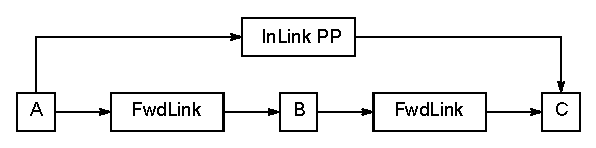
\includegraphics{lockScanProcess_6}

Assume that A, B, and C are all passive records. The notation states that A has a forward link to B and B to C. C has an 
input link obtaining a value from A. Assume, for some reason, A gets processed. The following sequence of events 
occurs:

\begin{enumerate}\item A begins processing. While processing a request is made to process B.

\item B starts processing. While processing a request is made to process C.

\item C starts processing. One of the first steps is to get a value from A via the input link.

\item At this point a question occurs. Note that the input link specifies process passive (signified by the \verb|PP| after 
\verb|InLink|). But process passive states that A should be processed before the value is retrieved. Are we in an infinite 
loop? The answer is no. Every record contains a field \verb|pact| (processing active), which is set \verb|TRUE| when record 
processing begins and is not set \verb|FALSE| until all processing completes. When C is processed A still has \verb|pact| \verb|TRUE| 
and will not be processed again.

\item C obtains the value from A and completes its processing. Control returns to B.

\item B completes returning control to A

\item A completes processing.

\end{enumerate}This brief example demonstrates that database links needs more discussion.

\subsection{Rules Relating to Database Links}

\subsubsection{Processing Order}

The processing order is guaranteed to follow the following rules:

\begin{enumerate}\item Forward links are processed in order from left to right and top to bottom. For example the following records are 
processed in the order \verb|FLNK1|, \verb|FLNK2|, \verb|FLNK3|, \verb|FLNK4| .

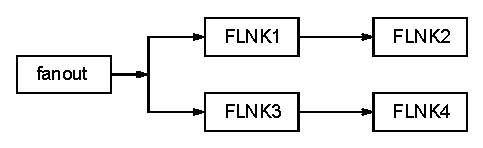
\includegraphics{lockScanProcess_9}

\item If a record has multiple input links (calculation and select records) the input is obtained in the natural order. For 
example if the fields are named \verb|INPA|, \verb|INPB|, ..., \verb|INPL|, then the links are read in the order A then B then C, etc. 
Thus if obtaining an input results in a record being processed, the processing order is guaranteed.

\item All input and output links are processed before the forward link.

\end{enumerate}\subsubsection{Lock Sets}

All records, except for the conditions listed in the next paragraph, linked together directly or indirectly are placed in the 
same lock set. When \verb|dbScanLock| is called the entire set, not just the specified record, is locked. This prevents two 
different tasks from simultaneously modifying records in the same lock set.

\subsubsection{PACT - processing active}

Each record contains a field \verb|pact|. This field is set \verb|TRUE| at the beginning of record processing and is not set \verb|FALSE| until 
the record is completely processed. In particular no links are processed with \verb|pact| \verb|FALSE|. This prevents infinite 
processing loops. The example given at the beginning of this section gives an example. It will be seen in the next two 
sections that \verb|pact| has other uses.

\subsubsection{Process Passive: Link option}

Input and output links have an option called process passive. For each such link the application developer can specify 
process passive \verb|TRUE| (\verb|PP|) or process passive \verb|FALSE| (\verb|NPP|). Consider the following example 

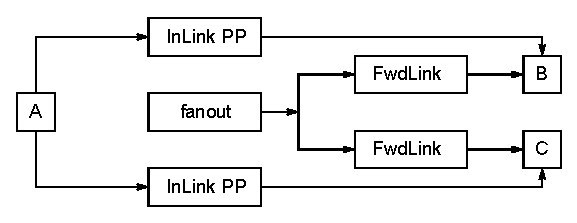
\includegraphics{lockScanProcess_16}

Assume that all records except fanout are passive. When the fanout record is processed the following sequence of events 
occur:

\begin{enumerate}\item Fanout starts processing and asks that B be processed.

\item B begins processing. It calls \verb|dbGetLink| to obtain data from A.

\item Because the input link has process passive true, a request is made to process A.

\item A is processed, the data value fetched, and control is returned to B

\item B completes processing and control is returned to fanout. Fanout asks that C be processed.

\item C begins processing. It calls \verb|dbGetLink| to obtain data from A.

\item Because the input link has process passive \verb|TRUE|, a request is made to process A.

\item A is processed, the data value fetched, and control is returned to C.

\item C completes processing and returns to fanout

\item The fanout completes

\end{enumerate}Note that A got processed twice. This is unnecessary. If the input link to C is declared no process passive then A will only 
be processed once. Thus we should have .

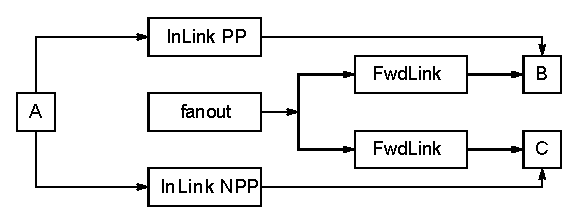
\includegraphics{lockScanProcess_26}

\subsubsection{Process Passive: Field attribute }

Each field of each database record type has an attribute called \verb|process_passive|. This attribute is specified in the  
record definition file. It is not under the control of the application developer. This attribute is used only by \verb|dbPutField|. 
It determines if a passive record will be processed after \verb|dbPutField| changes a field in the record. Consult the record 
specific information in the record reference manual for the setting of individual fields.

\subsubsection{Maximize Severity: Link option}

Input and output links have an option called maximize severity. For each such link the application developer can specify 
maximize severity \verb|TRUE| (\verb|MS|) or maximize severity \verb|FALSE| (\verb|NMS|). 

When database input or output links are defined, the application developer can specify if alarm severities should be 
propagated across links. For input links the severity is propagated from the record referred to by the link to the record 
containing the link. For output links the severity of the record containing the link is propagated to the record referenced by 
the link. The alarm severity is transferred only if the new severity will be greater than the current severity. If the severity 
is propagated the alarm status is set equal to \verb|LINK_ALARM|.

\section{Guidelines for Synchronous Records}

\index{Guidelines for Synchronous Records}A synchronous record is a record that can be completely processed without waiting. Thus the application developer never 
needs to consider the possibility of delays when he defines a set of related records. The only consideration is deciding 
when records should be processed and in what order a set of records should be processed.

The following reviews the methods available to the application programmer for deciding when to process a record and for 
enforcing the order of record processing.

\begin{enumerate}\item A record can be scanned periodically (at one of several rates), via I/O event, or via Event.

\item For each periodic group and for each Event group the phase field can be used to specify processing order.

\item The application programmer has no control over the record processing order of records in different groups.

\item The disable fields (\verb|SDIS|, \verb|DISA|, and \verb|DISV|) can be used to disable records from being processed. By letting the 
\verb|SDIS| field of an entire set of records refer to the same input record, the entire set can be enabled or disabled 
simultaneously. See the Record Reference Manual for details.

\item A record (periodic or other) can be the root of a set of passive records that will all be processed whenever the root 
record is processed. The set is formed by input, output, and forward links.

\item The \verb|process_passive| option specified for each field of each record determines if a passive record is processed 
when a \verb|dbPutField| is directed to the field. The application developer must be aware of the possibility of record 
processing being triggered by external sources if \verb|dbPutFields| are directed to fields that have 
\verb|process_passive| \verb|TRUE|.

\item The \verb|process_passive| option for input and output links provides the application developer control over how a 
set of records are scanned.

\item General link structures can be defined. The application programmer should be wary, however, of defining arbitrary 
structures without carefully analyzing the processing order. 

\end{enumerate}\section{Guidelines for Asynchronous Records}

\index{Guidelines for Asynchronous Records}The previous discussion does not allow for asynchronous records. An example is a GPIB input record. When the record is 
processed the GPIB request is started and the processing routine returns. Processing, however, is not really complete until 
the GPIB request completes. This is handled via an asynchronous completion routine. Lets state a few attributes of 
asynchronous record processing. 

During the initial processing for all asynchronous records the following is done:

\begin{enumerate}\item \verb|pact| is set \verb|TRUE|

\item Data is obtained for all input links

\item Record processing is started

\item The record processing routine returns

\end{enumerate}The asynchronous completion routine performs the following algorithm:

\begin{enumerate}\item Record processing continues

\item Record specific alarm conditions are checked

\item Monitors are raised

\item Forward links are processed

\item \verb|pact| is set \verb|FALSE|.

\end{enumerate}A few attributes of the above rules are:

\begin{enumerate}\item Asynchronous record processing does not delay the scanners.

\item Between the time record processing begins and the asynchronous completion routine completes, no attempt will be 
made to again process the record. This is because \verb|pact| is \verb|TRUE|. The routine \verb|dbProcess| checks \verb|pact| and does 
not call the record processing routine if it is \verb|TRUE|. Note, however, that if \verb|dbProcess| finds the record active 10 
times in succession, it raises a \verb|SCAN_ALARM|.

\item Forward and output links are triggered only when the asynchronous completion routine completes record 
processing.

\end{enumerate}With these rules the following works just fine:

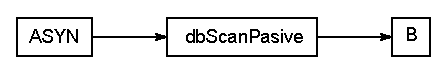
\includegraphics{lockScanProcess_34}

When \verb|dbProcess| is called for record ASYN, processing will be started but \verb|dbScanPassive| will not be called. Until 
the asynchronous completion routine executes any additional attempts to process ASYN are ignored. When the 
asynchronous callback is invoked the \verb|dbScanPassive| is performed.

Problems still remain. A few examples are:

\subsection{Infinite Loop}

\index{Infinite Loop}Infinite processing loops are possible.

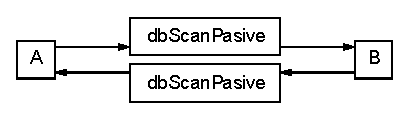
\includegraphics{lockScanProcess_1}

Assume both A and B are asynchronous passive records and a request is made to process A. The following sequence of 
events occur.

\begin{enumerate}\item A starts record processing and returns leaving \verb|pact| \verb|TRUE|.

\item Sometime later the record completion for A occurs. During record completion a request is made to process B. B 
starts processing and control returns to A which completes leaving its \verb|pact| field \verb|FALSE|.

\item Sometime later the record completion for B occurs. During record completion a request is made to process A. A 
starts processing and control returns to B which completes leaving its \verb|pact| field \verb|FALSE|.

\end{enumerate}Thus an infinite loop of record processing has been set up. It is up to the application developer to prevent such loops.

\subsection{Obtain Old Data}

A \verb|dbGetLink| to a passive asynchronous record can get old data.

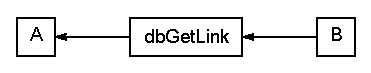
\includegraphics{lockScanProcess_37}

If A is a passive asynchronous record then the \verb|dbGetLink| request forces \verb|dbProcess| to be called for A. \verb|dbProcess| 
starts the processing and returns. \verb|dbGetLink| then reads the desired value which is still old because processing will only 
be completed at a later time.

\subsection{Delays}

Consider the following:

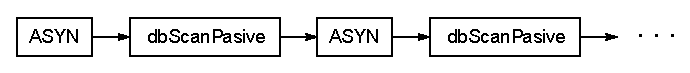
\includegraphics{lockScanProcess_40}

The second ASYN record will not begin processing until the first completes, etc. This is not really a problem except that 
the application developer must be aware of delays caused by asynchronous records. Again, note that scanners are not 
delayed, only records downstream of asynchronous records. 

\subsection{Task Abort}

If the processing task aborts and the watch dog task cleans up before the asynchronous processing routine completes what 
happens? If the asynchronous routine completes before the watch dog task runs everything is okay. If it doesn't? This is a 
more general question of the consequences of having the watchdog timer restart a scan task. EPICS currently does not 
allow scanners to be automatically restarted. 

\section{Cached Puts}

\index{Cached Puts}The rules followed by \verb|dbPutLink| and \verb|dbPutField| provide for ``cached" puts. This is necessary because of 
asynchronous records. Two cases arise.

The first results from a \verb|dbPutField|, which is a put coming from outside the database, i.e. Channel Access puts. If this 
is directed to a record that already has \verb|pact| \verb|TRUE| because the record started processing but asynchronous completion 
has not yet occurred, then a value is written to the record but nothing will be done with the value until the record is again 
processed. In order to make this happen \verb|dbPutField| arranges to have the record reprocessed when the record finally 
completes processing.

The second case results from \verb|dbPutLink| finding a record already active because of a \verb|dbPutField| directed to the 
record. In this case \verb|dbPutLink| arranges to have the record reprocessed when the record finally completes processing. If 
the record is already active because it appears twice in a chain of record processing, it is not reprocessed because the chain 
of record processing would constitute an infinite loop.

Note that the term caching not queuing is used. If multiple requests are directed to a record while it is active, each new 
value is placed in the record but it will still only be processed once, i.e. last value wins.

\section{putNotify}

\index{putNotify}\index{dbPutNotify}dbPutNotify, which is called when a Channel Access client calls \index{ca\_put\_callback}ca\_put\_callback, is a request to notify the caller when all 
records processed as a result of the put complete. Because of asynchronous records this can be complicated and the set of 
records that are processed because of a put may not be deterministic. The result of a dbPutNotify is the same as a 
dbPutField except for the following:

\begin{itemize}\item dbPutNotifys are queued rather than cached. Thus when additional dbPutNotifys are directed to a record that 
already has an active dbPutNotify, they are queued. As each one finishes it releases the next one in the queue.

\item If a dbPutNotify links to a record that is not active but has a dbPutNotify attached to it, no attempt is made to 
process the record.

\end{itemize}\section{Channel Access Links}

A channel access link is:

\begin{enumerate}\item A record link that references a record in a different IOC.

\item A link that the application developer forces to be a channel access link.

\end{enumerate}A channel access client task (dbCa)  handles all I/O for channel access links. It does the following:

\begin{itemize}\item At IOC initialization dbCa issues channel access search requests for each channel access link.

\item For each input link it establishes a channel access monitor. It uses \verb|ca_field_type| and \verb|ca_element_count| 
when it establishes the monitor. It also monitors the alarm status. Whenever the monitor is invoked the new data is 
stored in a buffer belonging to dbCa. When iocCore or the record support module asks for data the data is taken 
from the buffer and converted to the requested type.

\item For each output link, a buffer is allocated the first time iocCore/record support issues a put and a channel access 
connection has been made. This buffer is allocated according to  \verb|ca_field_type| and \verb|ca_element_count|. 
Each time iocCore/record support issues a put, the data is converted and placed in the buffer and a request is made 
to dbCa to issue a new ca\_put.

\end{itemize}Even if a link references a record in the same IOC it can be useful to force it to act like a channel access link. In particular 
the records will not be forced to be in the same lock set. As an example consider a scan record that links to a set of 
unrelated records, each of which can cause a lot of records to be processed. It is often NOT desirable to force all these 
records into the same lock set. Forcing the links to be handled as channel access links solves the problem.

CA links which connect between IOCs incur the extra overhead associated with message passing protocols, operating 
system calls, and network activity. In contrast, CA links which connect records in the same IOC are executed more 
efficiently by directly calling database access functions such as dbPutField() and dbGetField(), or by receiving callbacks 
directly from a database monitor subscription event queue.

Because channel access links interact with the database only via dbPutField, dbGetField, and a database monitor 
subscription event queue, their interaction with the database is fundamentally different from database links which are 
tightly integrated within the code that executes database records. For this reason and because channel access does not 
understand process passive or maximize severity, the semantics of channel access links are not the same as database links. 
Let's discuss the channel access semantics of INLINK, OUTLINK, and FWDLINK separately.

\subsection{INLINK}

The options for process passive are:

\begin{itemize}\item PP or NPP - This link is made a channel access link because the referenced record is not found in the local IOC. It 
is not possible to honor PP, thus the link always acts like NPP.

\item CA - Force the link to be a channel access link.

\item CP - Force the link to be a channel access link and also request that the record containing the link be processed 
whenever a monitor occurs.

\item CPP - Force the link to be a channel access link and also request that the record containing the link, if it is passive, 
be processed whenever a monitor occurs.

\end{itemize}Maximize Severity is honored.

\subsection{OUTLINK}

The options for process passive are:

\begin{itemize}\item PP or NPP - This link is made a channel access link because the referenced record is not found in the local IOC. It 
is not possible to honor PP thus the link always acts like NPP.

\item CA - Force the link to be a channel access link.

\end{itemize}Maximize Severity is not honored.

\subsection{FWDLINK}

A channel access forward link is honored only if it references the PROC field of a record. In that case a ca\_put with a 
value of 1 is written each time a forward link request is issued.

The options for process passive are:

\begin{itemize}\item PP or NPP - This link is made a channel access link because the referenced record is not found in the local IOC. It 
is not possible to honor PP thus it always acts like NPP.

\item CA - Force the link to be a channel access link.

\end{itemize}Maximize Severity is not honored.



\chapter{Database Definition}
\index{Database Definition}

\section{Overview}

This chapter describes \index{database definitions}database definitions. The following definitions are described:

\begin{itemize}
\item Menu
\item Record Type
\item Device
\item Driver
\item Registrar
\item Variable
\item Function
\item Breakpoint Table
\item Record Instance
\end{itemize}

Record Instances are fundamentally different from the other definitions. A file containing record instances should never 
contain any of the other definitions and vice-versa. Thus the following convention is followed:

\begin{description}
\index{Database Definition File}
\item [Database Definition File] A file that contains any type of definition except record instances.

\index{Record Instance File}
\item [Record Instance File] A file that contains only record instance definitions.
\end{description}

This chapter also describes utility programs which operate on these definitions

Any combination of definitions can appear in a single file or in a set of files related to each other via include files.

\section{Summary of Database Syntax}

\index{Database Format -- Summary}
The following summarizes the Database Definition syntax:

\begin{verbatim}
path "path"
addpath "path"
include "filename"
#comment
menu(name) {
    include "filename"
    choice(choice_name, "choice_value")
    ...
}

recordtype(record_type) {
    include "filename"
    field(field_name, field_type) {
        asl(asl_level)
        initial("init_value")
        promptgroup(gui_group)
        prompt("prompt_value")
        special(special_value)
        pp(pp_value)
        interest(interest_level)
        base(base_type)
        size(size_value)
        extra("extra_info")
        menu(name)
    }
    %C_declaration
    ...
}

device(record_type, link_type, dset_name, "choice_string")

driver(drvet_name)

registrar(function_name)

variable(variable_name)

breaktable(name) {
    raw_value eng_value
    ...
}
\end{verbatim}

The Following defines a Record Instance

\begin{verbatim}
record(record_type, record_name) {
include "filename"
field(field_name, "value")
    alias(alias_name)
    info(info_name, "value")
    ...
}
alias(record_name,alias_name)
\end{verbatim}

\section{General Rules for Database Definition}

\subsection{Keywords}

\index{Keywords}
The following are keywords, i.e. they may not be used as values unless they are enclosed in quotes:

\index{path}
\index{addpath}
\index{include}
\index{menu}
\index{choice}
\index{recordtype}
\index{field}
\index{device}
\index{driver}
\index{registrar}
\index{function}
\index{variable}
\index{breaktable}
\index{record}
\index{grecord}
\index{info}
\index{alias}
\begin{verbatim}
path
addpath
include
menu
choice
recordtype
field
device
driver
registrar
function
variable
breaktable
record
grecord
info
alias
\end{verbatim}

\subsection{Unquoted Strings}

\index{Unquoted String}
In the summary section, some values are shown as quoted strings and some unquoted. The actual rule is that any string 
consisting of only the following characters does not have to be quoted unless it contains one of the above keywords:

\begin{verbatim}
a-z A-Z 0-9 _ + - : . [ ] < > ;
\end{verbatim}

These are all legal characters for process variable names, although \verb|.| is
not allowed in a record name since it separates the record from the field name
in a PV name. Thus in many cases quotes are not needed around record or field
names in database files. Any string containing a macro does need to be quoted
though.

\subsection{Quoted Strings}

\index{Quoted String}
A quoted string can contain any ascii character except the quote character \verb|"|. The quote character itself can given by using \verb|\| as an escape. For example \verb|"\""| is a quoted string containing the single character \verb|"|.

\subsection{Macro Substitution}

\index{Macro Substitution}
Macro substitutions are permitted inside quoted strings. Macro instances take the form:

\begin{verbatim}
$(name)
\end{verbatim}

or

\begin{verbatim}
${name}
\end{verbatim}

There is no distinction between the use of parentheses or braces for delimiters, although the two must match for a given 
macro instance. The macro name can be made up from other macros, for example:

\begin{verbatim}
$(name_$(sel))
\end{verbatim}

A macro instance can also provide a default value that is used when no macro with the given name is defined. The default 
value can be defined in terms of other macros if desired, but cannot contain any unescaped comma characters. The syntax 
for specifying a default value is as follows:

\begin{verbatim}
$(name=default)
\end{verbatim}

Finally macro instances can also contain definitions of other macros, which can (temporarily) override any existing values 
for those macros but are in scope only for the duration of the expansion of this macro instance. These definitions consist 
of \verb|name=value| sequences separated by commas, for example:

\begin{verbatim}
$(abcd=$(a)$(b)$(c)$(d),a=A,b=B,c=C,d=D)
\end{verbatim}

\subsection{Escape Sequences}

\index{Escape Sequence}
The database routines translate standard C escape sequences inside database field value strings only. The standard C 
escape sequences supported are:

\begin{verbatim}
\a \b \f \n \r \t \v \\ \? \' \" \ooo \xhh
\end{verbatim}

\verb|\ooo| represents an octal number with 1, 2, or 3 digits. \verb|\xhh| represents a hexadecimal number with 1 or 2 digits.

\subsection{Comments}

\index{comment -- Database Definitions}
The comment symbol is ``\#''. Whenever the comment symbol appears, it and all characters through the end of the line are ignored.

\subsection{Define before referencing}

No item can be referenced until it is defined. For example a \verb|recordtype| menu field can not reference a menu unless 
that menu definition has already been defined. Another example is that a record instance can not appear until the 
associated record type has been defined.

\subsection{Multiple Definitions}

\index{Multiple Definitions}
If a menu, recordtype, device, driver, or breakpoint table is defined more than once, then only the first instance is used. 
Record instance definitions however are (normally) cumulative, so multiple instances of the same record may be loaded 
and each time a field value is encountered it replaces the previous value.

\subsection{Filename Extensions}

\index{filename extension conventions}
By convention:

\begin{itemize}
\item Record instances files have the extension ``\verb|.db|'' or ``\verb|.vdb|'' if the file also contains visual layout information

\item Database definition files have the extension ``\verb|.dbd|''

\end{itemize}

\section{\texttt{path addpath} -- Path Definition}

\index{path -- Database Definitions}
\index{addpath -- Database Definitions}
\subsection{Format}

\begin{verbatim}
path "dir:dir...:dir"
addpath "dir:dir...:dir"
\end{verbatim}

The path string follows the standard convention for the operating system, i.e. directory names are separated by a colon ``\verb|:|'' on Unix
and a semicolon ``\verb|;|'' on Windows.

The \verb|path| command specifies the current search path for use when loading database and database definition files.
The \verb|addpath| appends directory names to the current path.
The path is used to locate the initial database file and included files.
An empty \verb|dir| at the beginning, middle, or end of a non-empty path string means the current directory.
For example:

\begin{verbatim}
 nnn::mmm    # Current directory is between nnn and mmm
 :nnn        # Current directory is first
 nnn:        # Current directory is last
\end{verbatim}

Utilities which load database files (\verb|dbExpand|, \verb|dbLoadDatabase|, etc.) allow the user to specify an initial path. The 
\verb|path| and \verb|addpath| commands can be used to change or extend the initial path.

The initial path is determined as follows:

\begin{description}
\item If an initial path is specified, it is used. Else:

\item If the environment variable \verb|EPICS_DB_INCLUDE_PATH| is defined, it is used. Else:

\item the default path is ``\verb|.|'', i.e. the current directory.
\end{description}

The path is used unless the filename contains a \verb|/| or \verb|\|.
The first directory containing the specified filename is used.

\section{\texttt{include} -- Include File}

\index{include -- Database Definitions}
\subsection{Format}

\begin{verbatim}
include "filename"
\end{verbatim}

An include statement can appear at any place shown in the summary.
It uses the path as specified above.

\section{\texttt{menu} -- Menu Declaration}

\index{menu -- Database Definitions}
\subsection{Format}

\begin{verbatim}
menu(name) {
    choice(choice_name, "choice_string")
    ...
}
\end{verbatim}

\subsection{Definitions}

\begin{description}
\item [name] Name for menu. This is the unique name identifying the menu.
If duplicate definitions are specified, only the first is used.

\item [choice\_name] The name used in the \verb|enum| generated by \verb|dbToMenuH| or \verb|dbToRecordtypeH|.
This must be a legal C/C++ identifier.

\item [choice\_string] The text string associated with this particular choice.
\end{description}

\subsection{Example}

\begin{verbatim}
menu(menuYesNo) {
    choice(menuYesNoNO, "NO")
    choice(menuYesNoYES, "YES")
}
\end{verbatim}

\section{\texttt{recordtype} -- Record Type Declaration}

\index{record type -- Database Definitions}
\subsection{Format}

\begin{verbatim}
recordtype(record_type) {
    field(field_name, field_type) {
        asl(as_level)
        initial("init_value")
        promptgroup(gui_group)
        prompt("prompt_value")
        special(special_value)
        pp(pp_value)
        interest(interest_level)
        base(base_type)
        size(size_value)
        extra("extra_info")
        menu("name")
    }
    %C_declaration
    ...
}
\end{verbatim}

\subsection{Field Definition Rules}

\index{field definition rules}
\begin{description}

\index{asl -- field definition rules}
\item [asl] Sets the Access Security Level for the field.
Access Security is discussed in chapter \ref{Access Security}.

\index{initial -- field definition rules}
\item [initial] Provides an initial (default) value for the field.

\index{promptgroup -- field definition rules}
\item [promptgroup] The group to which the field belongs, for database configuration tools.

\index{prompt -- field definition rules}
\item [prompt] A prompt string for database configuration tools.
Optional if \verb|promptgroup| is not defined.

\index{special -- field definition rules}
\item [special] If specified, special processing is required for this field at run time.

\index{pp -- field definition rules}
\item [pp] Whether a passive record should be processed when Channel Access writes to this field.

\index{interest -- field definition rules}
\item [interest] Interest level for the field.

\index{base -- field definition rules}
\item [base] For integer fields, the number base to use when converting the field value to a string.

\index{size -- field definition rules}
\item [size] Must be specified for \verb|DBF_STRING| fields.

\index{extra -- field definition rules}
\item [extra] Must be specified for \verb|DBF_NOACCESS| fields.

\index{menu -- field definition rules}
\item [menu] Must be specified for \verb|DBF_MENU| fields. It is the name of the associated menu.
\end{description}

\subsection{Definitions}

\begin{description}
\index{record\_type -- record type definition}
\item [record\_type] The unique name of the record type.
If duplicates are specified, only the first definition is used.

\index{field\_name -- field definition}
\item [field\_name] The field name, which must be a valid C identifier.
When include files are generated, the field name is converted to lower case.
Previous versions of EPICS required the field name be a maximum of four characters, but this restriction no longer applies.

\index{field\_type -- field definition}
\item [field\_type] This must be one of the following values:

\begin{itemize}
\item \verb|DBF_STRING|
\item \verb|DBF_CHAR|, \verb|DBF_UCHAR|
\item \verb|DBF_SHORT|, \verb|DBF_USHORT|
\item \verb|DBF_LONG|, \verb|DBF_ULONG|
\item \verb|DBF_FLOAT|, \verb|DBF_DOUBLE|
\item \verb|DBF_ENUM|, \verb|DBF_MENU|, \verb|DBF_DEVICE|
\item \verb|DBF_INLINK|, \verb|DBF_OUTLINK|, \verb|DBF_FWDLINK|
\item \verb|DBF_NOACCESS|
\end{itemize}

\index{as\_level -- field definition}
\item [as\_level] This must be one of the following values:

\begin{itemize}
\item \verb|ASL0|
\item \verb|ASL1|  (default value)
\end{itemize}

Fields which operators normally change are assigned \verb|ASL0|.
Other fields are assigned \verb|ASL1|.
For example, the \verb|VAL| field of an analog output record is assigned \verb|ASL0| and all other fields \verb|ASL1|.
This is because only the \verb|VAL| field should be modified during normal operations.

\index{init\_value -- field definition}
\item [init\_value] A legal value for data type.

\index{prompt\_value -- field definition}
\item [prompt\_value] A prompt value for database configuration tools.

\index{gui\_group -- field definition}
\item [gui\_group] This must be one of the following:

\begin{itemize}
\item \verb|GUI_COMMON|
\item \verb|GUI_ALARMS|
\item \verb|GUI_BITS1|
\item \verb|GUI_BITS2|
\item \verb|GUI_CALC|
\item \verb|GUI_CLOCK|
\item \verb|GUI_COMPRESS|
\item \verb|GUI_CONVERT|
\item \verb|GUI_DISPLAY|
\item \verb|GUI_HIST|
\item \verb|GUI_INPUTS|
\item \verb|GUI_LINKS|
\item \verb|GUI_MBB|
\item \verb|GUI_MOTOR|
\item \verb|GUI_OUTPUT|
\item \verb|GUI_PID|
\item \verb|GUI_PULSE|
\item \verb|GUI_SELECT|
\item \verb|GUI_SEQ1|
\item \verb|GUI_SEQ2|
\item \verb|GUI_SEQ3|
\item \verb|GUI_SUB|
\item \verb|GUI_TIMER|
\item \verb|GUI_WAVE|
\item \verb|GUI_SCAN|

This information is for use by Database Configuration Tools.
This is defined only for fields that can be given values by database configuration tools.
File \verb|guigroup.h| contains all possible definitions.
This allows database configuration tools to group fields together by functionality, not just order them by name.
This feature has seldom been used, so many record types do not have appropriate values assigned to some fields.

\end{itemize}

\index{special\_value -- field definition}
\item [special\_value] Must be one of the following:

\begin{itemize}
\index{SPC\_MOD}
\item \verb|SPC_MOD| -- Notify record support when modified.
The record support \verb|special| routine will be called whenever the field is modified by the database access routines.

\index{SPC\_NOMOD}
\item \verb|SPC_NOMOD| -- No external modifications allowed.
This value disables external writes to the field, so it can only be set by the record or device support module.

\index{SPC\_DBADDR}
\item \verb|SPC_DBADDR| -- Use this if the record support \verb|cvt_dbaddr| routine should be called by \verb|dbNameToAddr|,
i.e. when code outside record/device support is connecting to the field.

The following values are for database common fields.
They must \emph{not} be used for record specific fields:

\index{SPC\_SCAN}
\item \verb|SPC_SCAN| -- Scan related field.

\index{SPC\_ALARMACK}
\item \verb|SPC_ALARMACK| -- Alarm acknowledgment field.

\index{SPC\_AS}
\item \verb|SPC_AS| -- Access security field.

The following values are deprecated, use \verb|SPC_MOD| instead:

\item An integer value greater than 103.

\index{SPC\_RESET}
\item \verb|SPC_RESET| -- a reset field is being modified.

\index{SPC\_LINCONV}
\item \verb|SPC_LINCONV| -- A linear conversion field is being modified.

\index{SPC\_CALC}
\item \verb|SPC_CALC| -- A calc field is being modified.
\end{itemize}

\index{pp\_value -- field definition}
\item [pp\_value] Should a passive record be processed when Channel Access writes to this field?
The allowed values are:

\begin{itemize}
\item \verb|NO| (default)
\item \verb|YES|
\end{itemize}

\index{interest\_level -- field definition}
\item [interest\_level] An interest level for the \verb|dbpr| command.

\index{base -- field definition}
\item [base] For integer type fields, the default base.
The legal values are:

\begin{itemize}
\item \verb|DECIMAL| (Default)
\item \verb|HEX|
\end{itemize}

\index{size\_value -- field definition}
\item [size\_value] The number of characters for a \verb|DBF_STRING| field.

\index{extra\_info -- field definition}
\item [extra\_info] For \verb|DBF_NOACCESS| fields, this is the C language definition for the field.
The definition must end with the fieldname in lower case.

\item [\%C\_declaration] A percent sign \verb|%| inside the record body introduces a line of code that is to be included in the generated C header file.
\end{description}

\subsection{Example}

The following is the definition of the event record type:

\begin{verbatim}
recordtype(event) {
    include "dbCommon.dbd" 
    field(VAL,DBF_USHORT) {
        prompt("Event Number To Post")
        promptgroup(GUI_INPUTS)
        asl(ASL0)
    }
    field(INP,DBF_INLINK) {
        prompt("Input Specification")
        promptgroup(GUI_INPUTS)
        interest(1)
    }
    field(SIOL,DBF_INLINK) {
        prompt("Sim Input Specifctn")
        promptgroup(GUI_INPUTS)
        interest(1)
    }
    field(SVAL,DBF_USHORT) {
        prompt("Simulation Value")
    }
    field(SIML,DBF_INLINK) {
        prompt("Sim Mode Location")
        promptgroup(GUI_INPUTS)
        interest(1)
    }
    field(SIMM,DBF_MENU) {
        prompt("Simulation Mode")
        interest(1)
        menu(menuYesNo)
    }
    field(SIMS,DBF_MENU) {
        prompt("Sim mode Alarm Svrty")
        promptgroup(GUI_INPUTS)
        interest(2)
        menu(menuAlarmSevr)
    }
}
\end{verbatim}

\section{\texttt{device} -- Device Support Declaration}

\index{device -- Database Definitions}
\subsection{Format}

\begin{verbatim}
    device(record_type, link_type, dset_name, "choice_string")
\end{verbatim}

\subsection{Definitions}

\begin{description}
\index{record\_type -- device definition}
\item [record\_type] Record type.
The combination of \verb|record_type| and \verb|choice_string| must be unique.
If the same combination appears more than once, only the first definition is used.

\index{link\_type -- device definition}
\item [link\_type] Link type. This must be one of the following:

\begin{itemize}
\item \verb|CONSTANT|
\item \verb|PV_LINK|
\item \verb|VME_IO|
\item \verb|CAMAC_IO|
\item \verb|AB_IO|
\item \verb|GPIB_IO|
\item \verb|BITBUS_IO|
\item \verb|INST_IO|
\item \verb|BBGPIB_IO|
\item \verb|RF_IO|
\item \verb|VXI_IO|
\end{itemize}

\index{dset\_name -- device definition}
\item [dset\_name] The name of the device support entry table for this device support.

\index{choice\_string -- device definition}
\item [choice\_string] The \verb|DTYP| choice string for this device support.
A \verb|choice_string| value may be reused for different record types, but must be unique for each specific record type.
\end{description}

\subsection{Examples}

\begin{verbatim}
    device(ai,CONSTANT,devAiSoft,"Soft Channel")
    device(ai,VME_IO,devAiXy566Se,"XYCOM-566 SE Scanned")
\end{verbatim}

\section{\texttt{driver} -- Driver Declaration}

\index{driver -- database definition}
\subsection{Format}

\begin{verbatim}
    driver(drvet_name)
\end{verbatim}

\subsection{Definitions}

\begin{description}
\index{drvet\_name -- driver definition}
\item [drvet\_name] If duplicates are defined, only the first is used.

\end{description}

\subsection{Examples}

\begin{verbatim}
    driver(drvVxi)
    driver(drvXy210)
\end{verbatim}

\section{\texttt{registrar} -- Registrar Declaration}

\index{registrar -- Database Defintions}
\subsection{Format}

\begin{verbatim}
    registrar(function_name)
\end{verbatim}

\subsection{Definitions}

\begin{description}
\index{function\_name -- registrar definition}
\item [function\_name] The name of an C function that accepts no arguments, returns \verb|void| and has been marked in
its source file with an \index{epicsExportRegistrar}\verb|epicsExportRegistrar| declaration, e.g.
\end{description}

\begin{verbatim}
    static void myRegistrar(void);
    epicsExportRegistrar(myRegistrar);
\end{verbatim}

This can be used to register functions for use by subroutine records or that can be invoked from iocsh. The example 
application described in Section \ref{Example IOC Application}, ``Example IOC Application'' on page \pageref{Example IOC Application}
gives an example of how to register functions for subroutine records.

\subsection{Example}

\begin{verbatim}
    registrar(myRegistrar)
\end{verbatim}

\section{\texttt{variable} -- Variable Declaration}

\index{variable -- Database Definitions}
\subsection{Format}

\begin{verbatim}
    variable(variable_name[, type])
\end{verbatim}

\subsection{Definitions}

\begin{description}
\index{variable\_name -- variable definition}
\item [variable\_name] The name of a C variable which has been marked in its source file with an 
\index{epicsExportAddress}\verb|epicsExportAddress| declaration.

\index{type -- variable definition}
\item [type] The C variable's type.
If not present, \verb|int| is assumed.
Currently only \verb|int| and \verb|double| variables are supported.
\end{description}

This registers a diagnostic/configuration variable for device or driver support or a subroutine record subroutine so that
the variable can be read and set with the iocsh \verb|var| command (see Section \ref{Utility Commands} on page \pageref{Utility Commands}).
The example application described in Section \ref{Example IOC Application} on page \pageref{Example IOC Application}
provides an example of how to register a debug variable for a subroutine record.

\subsection{Example}

In an application C source file:

\begin{verbatim}
    #include <epicsExport.h>

    static double myParameter;
    epicsExportAddress(double, myParameter);
\end{verbatim}

In an application database definition file:

\begin{verbatim}
    variable(myParameter, double)
\end{verbatim}

\section{\texttt{function} -- Function Declaration}

\index{function -- Database Definitions}
\subsection{Format}

\begin{verbatim}
function(function_name)
\end{verbatim}

\subsection{Definitions}

\begin{description}
\index{function\_name -- function definition}
\item [function\_name] The name of a C function which has been exported from its source file with an
\index{epicsRegisterFunction}\verb|epicsRegisterFunction| declaration.
\end{description}

This registers a function so that it can be found in the function registry for use by record types such as sub or aSub which 
refer to the function by name. The example application described in Section \ref{Example IOC Application} on page \pageref{Example IOC Application}
provides an example of how to register functions for a subroutine record.

\subsection{Example}

In an application C source file:

\begin{verbatim}
    #include <epicsExport.h>
    #include <registryFunction.h>

    static long myFunction(void *argp) {
        /* my code ... */
    }
    epicsRegisterFunction(myFunction);
\end{verbatim}

In an application database definition file:

\begin{verbatim}
    function(myFunction)
\end{verbatim}

\section{\texttt{breaktable} -- Breakpoint Table}

\index{breakpoint table -- Database Definitions}
\index{breaktable}
\subsection{Format}

\begin{verbatim}
breaktable(name) {
    raw_value eng_value
    ...
}
\end{verbatim}

\subsection{Definitions}

\begin{description}
\index{name -- breakpoint table}
\item [name] Name, which must be alpha-numeric, of the breakpoint table.
If duplicates are specified the first is used.

\index{raw\_value -- breakpoint table}
\item [raw\_value] The raw value, i.e. the actual ADC value associated with the beginning of the interval.

\index{eng\_value -- breakpoint table}
\item [eng\_value] The engineering value associated with the beginning of the interval.
\end{description}

\subsection{Example}

\begin{verbatim}
breaktable(typeJdegC) {
    0.000000 0.000000
    365.023224 67.000000
    1000.046448 178.000000
    3007.255859 524.000000
    3543.383789 613.000000
    4042.988281 692.000000
    4101.488281 701.000000
}
\end{verbatim}

\section{\texttt{record} -- Record Instance}

\index{record instance -- Database Definitions}
\index{record}
\subsection{Format}

\begin{verbatim}
record(record_type, record_name) {
    alias(alias_name)
    field(field_name, "field_value")
    info(info_name, "info_value")
    ...
}
alias(record_name, alias_name)
\end{verbatim}

\subsection{Definitions}

\begin{description}
\index{record\_type -- record instance definition}
\item [record\_type] The record type.

\index{record\_name -- record instance definition}
\item [record\_name] The record name.
This must be composed of the following characters:

\begin{verbatim}
    a-z A-Z 0-9 _ - + : [ ] < > ;
\end{verbatim}

NOTE: If macro substitutions are used the name must be quoted.

Duplicate definitions are normally allowed for a record as long as the record type is the same.
The last value given for each field is the value used.

\index{dbRecordsOnceOnly}
The variable \verb|dbRecordsOnceOnly| can be set to any non-zero value using the iocsh \verb|var| command to make loading duplicate record definitions into the IOC illegal.

\index{alias\_name -- record instance definition}
\item [alias\_name] An alternate name for the record, following the same rules as the record name.

\index{field\_name -- record instance definition}
\item [field\_name] A field name.

\index{field value -- record instance definition}
\item [field\_value] A value for the named field, depending on the particular field type.
Inside double quotes the field value string may contain escaped C89 characters such as 
\verb|\"|, \verb|\t|, \verb|\n|, \verb|\064| and \verb|\x7e|, and these will be translated appropriately when loading the database.
Permitted values are as follows:

\begin{itemize}
\item \verb|DBF_STRING| \\
Any ASCII string. If it exceeds the field length, it will be truncated.

\item \verb|DBF_CHAR|, \verb|DBF_UCHAR|, \verb|DBF_SHORT|, \verb|DBF_USHORT|, \verb|DBF_LONG|, \verb|DBF_ULONG| \\
A string that represents a valid integer. The standard C conventions are applied, i.e. a leading 0 means the 
value is given in octal and a leading 0x means that value is given in hex.

\item \verb|DBF_FLOAT|, \verb|DBF_DOUBLE| \\
The string must represent a valid floating point number.

\item \verb|DBF_MENU| \\
The string must be one of the valid choices for the associated menu.

\item \verb|DBF_DEVICE| \\
The string must be one of the valid device choice strings.

\item \verb|DBF_INLINK|, \verb|DBF_OUTLINK|, \verb|DBF_FWDLINK| \\
NOTES:

\begin{itemize}
\item If the field name is \verb|INP| or \verb|OUT| then this field is associated with \verb|DTYP|, and the permitted values
are determined by the link type of the device support selected by the current \verb|DTYP| choice string.
Other \verb|DBF_INLINK| and \verb|DBF_OUTLINK| fields must be either \verb|CONSTANT| or \verb|PV_LINK|s.

\item A device support that specifies a link type of \verb|CONSTANT| can be given either a constant or a \verb|PV_LINK|.
\end{itemize}

The allowed values for the field depend on the device support's link type as follows:

\begin{itemize}
\item \verb|CONSTANT| \\
\index{CONSTANT -- link field value}
A numeric literal, valid for the field type it is to be read into.

\item \verb|PV_LINK| \\
\index{PV\_LINK -- link field value}
A value of the form:

\begin{verbatim}
    record.field process maximize
\end{verbatim}

\verb|record| is the name of a record that exists in this or another IOC.

The \verb|.field|, \verb|process|, and \verb|maximize| parts are all optional.

The default value for \verb|.field| is \verb|.VAL|.

\verb|process| can have one of the following values:

\begin{itemize}
\item \verb|NPP| -- No Process Passive (Default)
\item \verb|PP| -- Process Passive
\item \verb|CA| -- Force link to be a channel access link
\item \verb|CP| -- CA and process on monitor
\item \verb|CPP| -- CA and process on monitor if record is passive

NOTES:

\verb|CP| and \verb|CPP| are valid only for \verb|DBF_INLINK| fields.

\verb|DBF_FWDLINK| fields can use \verb|PP| or \verb|CA|.
If a \verb|DBF_FWDLINK| is a channel access link it must reference the target record's \verb|PROC| field.
\end{itemize}

\verb|maximize| can have one of the following values:

\begin{itemize}
\item \verb|NMS| -- No Maximize Severity (Default)
\item \verb|MS| -- Maximize Severity
\item \verb|MSS| -- Maximize Severity and Status
\item \verb|MSI| -- Maximize Severity if Invalid
\end{itemize}

\index{VME\_IO -- link field value}
\item \verb|VME_IO| \\
\verb|#Ccard Ssignal @parm|

\verb|card| -- the card number of associated hardware module \\
\verb|signal| -- signal on card \\
\verb|parm| -- An arbitrary character string of up to 31 characters. This field is optional and is device specific.

\item \verb|CAMAC_IO| \\
\index{CAMAC\_IO -- link field value}
\verb|#Bbranch Ccrate Nstation Asubaddress Ffunction @parm|

\verb|branch|, \verb|crate|, \verb|station|, \verb|subaddress|, and \verb|function| should be obvious to \verb|camac| users.
\verb|subaddress| and \verb|function| are optional (0 if not given).
\verb|parm| is also optional and is device specific (25 characters max).

\item \verb|AB_IO| \\
\index{AB\_IO -- link field value}
\verb|#Llink Aadapter Ccard Ssignal @parm|

\verb|link| -- Scanner, i.e. vme scanner number \\
\verb|adapter| -- Adapter. Allen Bradley also calls this rack \\
\verb|card| -- Card within Allen Bradley Chassis \\
\verb|signal| -- signal on card \\
\verb|parm| -- optional device-specific character string (27 char max)

\item \verb|GPIB_IO| \\
\index{GPIB\_IO -- link field value}
\verb|#Llink Aaddr @parm|

\verb|link| -- gpib link, i.e. interface \\
\verb|addr| -- GPIB address \\
\verb|parm| -- device-specific character string (31 char max)

\item \verb|BITBUS_IO| \\
\index{BITBUS\_IO -- link field value}
\verb|#Llink Nnode Pport Ssignal @parm|

\verb|link| -- link, i.e.  vme bitbus interface \\
\verb|node| -- bitbus node \\
\verb|port| -- port on the node \\
\verb|signal| -- signal on port \\
\verb|parm| -- device specific-character string (31 char max)

\item \verb|INST_IO|
\index{INST\_IO -- link field value}
\verb|@parm|

\verb|parm| -- Device dependent character string

\item \verb|BBGPIB_IO| \\
\index{BBGPIB\_IO -- link field value}
\verb|#Llink Bbbaddr Ggpibaddr @parm|

\verb|link| -- link, i.e. vme bitbus interface \\
\verb|bbadddr| -- bitbus address \\
\verb|gpibaddr| -- gpib address \\
\verb|parm| -- optional device-specific character string (31 char max)

\item \verb|RF_IO| \\
\index{RF\_IO -- link field value}
\verb|#Rcryo Mmicro Ddataset Eelement|

\item \verb|VXI_IO| \\
\index{VXI\_IO -- link field value}
\verb|#Vframe Cslot Ssignal @parm| (Dynamic addressing) \\
     or \\
\verb|#Vla Signal @parm|  (Static Addressing)

\verb|frame| -- VXI frame number \\
\verb|slot| -- Slot within VXI frame \\
\verb|la| -- Logical Address \\
\verb|signal| -- Signal Number \\
\verb|parm| -- device specific character string(25 char max)
\end{itemize}
\end{itemize}

\index{info\_name -- record instance definition}
\item [info\_name] The name of an Information Item related to this record.
See section \ref{Record Information Item} below for more on Information Items.

\index{info\_value -- record instance definition}
\item [info\_value] Any ASCII string.
IOC applications using this information item may place additional restrictions on the contents of the string.

\end{description}

\subsection{Examples}

\begin{verbatim}
record(ai,STS_AbAiMaS0) {
    field(SCAN,".1 second")
    field(DTYP,"AB-1771IFE-4to20MA")
    field(INP,"#L0 A2 C0 S0 F0 @")
    field(PREC,"4")
    field(LINR,"LINEAR")
    field(EGUF,"20")
    field(EGUL,"4")
    field(EGU,"MilliAmps")
    field(HOPR,"20")
    field(LOPR,"4")
}
record(ao,STS_AbAoMaC1S0) {
    field(DTYP,"AB-1771OFE")
    field(OUT,"#L0 A2 C1 S0 F0 @")
    field(LINR,"LINEAR")
    field(EGUF,"20")
    field(EGUL,"4")
    field(EGU,"MilliAmp")
    field(DRVH,"20")
    field(DRVL,"4")
    field(HOPR,"20")
    field(LOPR,"4")
    info(autosaveFields,"VAL")
}
record(bi,STS_AbDiA0C0S0) {
    field(SCAN,"I/O Intr")
    field(DTYP,"AB-Binary Input")
    field(INP,"#L0 A0 C0 S0 F0 @")
    field(ZNAM,"Off")
    field(ONAM,"On")
}
\end{verbatim}

\section{Record Information Item}
\label{Record Information Item}

\index{Information item}
Information items provide a way to attach named string values to individual record instances that are loaded at the same time as the record definition.
They can be attached to any record without having to modify the record type, and can be retrieved by programs running on the IOC (they are not visible via Channel Access at all).
Each item attached to a single record must have a unique name by which it is addressed, and database access provides routines to allow a record's info items to be scanned, searched for, retrieved and set.
At runtime a \verb|void*| \index{Infomation item pointer}pointer can also be associated with each item, although only the string value can be initialized from the record definition when the database is loaded.

\section{Record Attributes}

\index{record attribute}
Each record type can have any number of record attributes.
Each attribute is a \index{Psuedo field}psuedo field that can be accessed via database and channel access.
Each attribute has a name that acts like a field name but returns the same value for all instances of the record type.
Two attributes are generated automatically for each record type: \verb|RTYP| and \verb|VERS|.
The value for \verb|RTYP| is the record type name.
The default value for \verb|VERS| is ``none specified'', which can be changed by record support.
Record support can call the following routine to create new attributes or change existing attributes:

\index{dbPutAttribute}
\begin{verbatim}
    long dbPutAttribute(char *recordTypename,
       char *name, char*value)
\end{verbatim}

The arguments are:

\begin{description}
\item \verb|recordTypename| -- The name of recordtype.
\item \verb|name| -- The attribute name, i.e. the psuedo field name.
\item \verb|value| -- The value assigned to the attribute.
\end{description}

\section{Breakpoint Tables -- Discussion}

\index{Breakpoint Tables}
\index{menuConvert}
\index{LINR}
The menu \verb|menuConvert| is used for field \verb|LINR| of the \verb|ai| and \verb|ao| records.
These records allow raw data to be converted to/from engineering units via one of the following:

\begin{enumerate}
\item No Conversion.
\item \index{Slope Conversion}Slope Conversion.
\item \index{Linear Conversion}Linear Conversion.
\item Breakpoint table.
\end{enumerate}

Other record types can also use this feature.
The first choice specifies no conversion; the second and third are both linear conversions, the difference being that for Slope conversion the user specifies the conversion slope and offset values directly, whereas for Linear conversions these are calculated by the device support from the requested Engineering Units range and the device support's knowledge of the hardware conversion range.
The remaining choices are assumed to be the names of breakpoint tables.
If a breakpoint table is chosen, the record support modules calls \verb|cvtRawToEngBpt| or \verb|cvtEngToRawBpt|.
You can look at the \verb|ai| and \verb|ao| record support modules for details.

If a user wants to add additional breakpoint tables, then the following should be done:

\begin{itemize}
\item Copy the \verb|menuConvert.dbd| file from EPICS \verb|base/src/bpt|
\item Add definitions for new breakpoint tables to the end
\item Make sure modified \verb|menuConvert.dbd| is loaded  into the IOC instead of EPICS version.
\end{itemize}

It is only necessary to load a breakpoint file if a record instance actually chooses it.
It should also be mentioned that the Allen Bradley IXE device support misuses the \verb|LINR| field.
If you use this module, it is very important that you do not change any of the EPICS supplied definitions in \verb|menuConvert.dbd|.
Just add your definitions at the end.

If a breakpoint table is chosen, then the corresponding breakpoint file must be loaded into the IOC before \verb|iocInit| is called.

Normally, it is desirable to directly create the breakpoint tables.
However, sometimes it is desirable to create a breakpoint table from a table of raw values representing equally spaced engineering units.
A good example is the Thermocouple tables in the OMEGA Engineering, INC Temperature Measurement Handbook.
A tool \index{makeBpt}\verb|makeBpt| is provided to convert such data to a breakpoint table.

The format for generating a breakpoint table from a data table of raw values corresponding to equally spaced engineering values is:

\begin{verbatim}
    !comment line
    <header line>
    <data table>
\end{verbatim}

The header line contains the following information:

\begin{description}
\item [Name] An alphanumeric ascii string specifying the breakpoint table name
\item [Low Value Eng] Engineering Units Value for first breakpoint table entry
\item [Low Value Raw] Raw value for first breakpoint table entry
\item [High Value Eng] Engineering Units: Highest Value desired
\item [High Value Raw] Raw Value for High Value Eng
\item [Error] Allowed error (Engineering Units)
\item [First Table] Engineering units corresponding to first data table entry
\item [Last Table] Engineering units corresponding to last data table entry
\item [Delta Table] Change in engineering units per data table entry
\end{description}

 An example definition is:

\begin{verbatim}
    "TypeKdegF" 32 0 1832 4095 1.0 -454 2500 1
    <data table>
\end{verbatim}

The breakpoint table can be generated by executing

\begin{verbatim}
    makeBpt bptXXX.data
\end{verbatim}

The input file must have the extension of data.
The output filename is the same as the input filename with the extension of \verb|.dbd|.

Another way to create the breakpoint table is to include the following definition in a \verb|Makefile|:

\begin{verbatim}
BPTS += bptXXX.dbd
\end{verbatim}

NOTE: This requires the naming convention that all data tables are of the form \verb|bpt<name>.data| and a breakpoint table \verb|bpt<name>.dbd|.

\section{Menu and Record Type Include File Generation.}

\index{Include File Generation}
\subsection{Introduction}

\index{dbToMenuH}
\index{dbToRecordtypeH}
Given a file containing menus, \verb|dbToMenuH| generates an include file that can be used by any code which uses the associated menus.
Given a file containing any combination of menu definitions and record type definitions, \verb|dbToRecordtypeH| generates an include file that can be used by any code which uses the menus and record type.

EPICS base uses the following conventions for managing menu and recordtype definitions.
Users generating local record types are encouraged to do likewise.

\begin{itemize}
\item Each menu that is either for fields in database common (for example \verb|menuScan|) or is of global use (for example \verb|menuYesNo|) is defined in a separate file.
The name of the file is the same as the menu name with an extension of \verb|.dbd|.
The name of the generated include file is the menu name with an extension of \verb|.h|.
Thus \verb|menuScan| is defined in a file \verb|menuScan.dbd| and the generated include file is named \verb|menuScan.h|

\item Each record type definition is defined in a separate file.
In addition, this file contains any menu definitions that are used only by that record type.
The name of the file is the same as the recordtype name followed by \verb|Record.dbd|.
The name of the generated include file is the same name with an extension of \verb|.h|.
Thus \verb|aoRecord| is defined in a file \verb|aoRecord.dbd| and the generated include file is named \verb|aoRecord.h|.
Since \verb|aoRecord| has a private menu called \verb|aoOIF|, the \verb|dbd| file and the generated include file have definitions for this menu.
Thus for each record type, there are two source files (\verb|xxxRecord.dbd| and \verb|xxxRecord.c|) and one generated file (\verb|xxxRecord.h|).
\end{itemize}

Before continuing, it should be mentioned that developers don't normally execute \verb|dbToMenuH| or \verb|dbToRecordtypeH| themselves.
If the proper naming conventions are used, it is only necessary to add definitions to the appropriate \verb|Makefile|.
Consult the chapter on the EPICS Build Facility for details.

\subsection{dbToMenuH}

\index{dbToMenuH}
This tool is executed as follows:

\begin{verbatim}
dbToMenuH -Idir -Smacsub menuXXX.dbd
\end{verbatim}

It generates a file which has the same name as the input file but with an extension of \verb|.h|.
Multiple \verb|-I| options can be specified for an include path and multiple \verb|-S| options for macro substitution.

For example \verb|menuPriority.dbd|, which contains the definitions for processing priority contains:

\begin{verbatim}
menu(menuPriority) {
    choice(menuPriorityLOW,"LOW")
    choice(menuPriorityMEDIUM,"MEDIUM")
    choice(menuPriorityHIGH,"HIGH")
}
\end{verbatim}

The include file, \verb|menuPriority.h|, generated by \verb|dbToMenuH| contains:

\begin{verbatim}
#ifndef INCmenuPriorityH
#define INCmenuPriorityH
typedef enum {
    menuPriorityLOW,
    menuPriorityMEDIUM,
    menuPriorityHIGH,
}menuPriority;
#endif /*INCmenuPriorityH*/

\end{verbatim}

Any code that needs to use the priority menu values should use these definitions.

\subsection{dbToRecordtypeH}

\index{dbToRecordtypeH}
This tool is executed as follows:

\begin{verbatim}
dbTorecordtypeH -Idir -Smacsub xxxRecord.dbd
\end{verbatim}

It generates a file which has the same name as the input file but with an extension of \verb|.h|.
Multiple \verb|-I| options can be specified for an include path and multiple \verb|-S| options for macro substitution.

For example \verb|aoRecord.dbd|, which contains the definitions for the analog output record contains:

\begin{verbatim}
menu(aoOIF) {
    choice(aoOIF_Full,"Full")
    choice(aoOIF_Incremental,"Incremental")
}
recordtype(ao) {
    include "dbCommon.dbd"
    field(VAL,DBF_DOUBLE) {
    prompt("Desired Output")
        asl(ASL0)
        pp(TRUE)
    }
    field(OVAL,DBF_DOUBLE) {
        prompt("Output Value")
    }
    ... (Many more field definitions
    }
}
\end{verbatim}

The include file, \verb|aoRecord.h|, generated by \verb|dbToRecordtypeH| contains:

\begin{verbatim}
#include "ellLib.h"
#include "epicsMutex.h"
#include "link.h"
#include "epicsTime.h"
#include "epicsTypes.h"

#ifndef INCaoOIFH
#define INCaoOIFH
typedef enum {
        aoOIF_Full,
        aoOIF_Incremental,
}aoOIF;
#endif /*INCaoOIFH*/
#ifndef INCaoH
#define INCaoH
typedef struct aoRecord {
        char            name[29]; /*Record Name*/
        ... Remaining fields in database common
        double          val;    /*Desired Output*/
        double          oval;   /*Output Value*/
        ... remaining record specific fields
} aoRecord;
#define aoRecordNAME    0
... defines for remaining fields in database common
#define aoRecordVAL     42
#define aoRecordOVAL    43
... defines for remaining record specific fields
#ifdef GEN_SIZE_OFFSET
int aoRecordSizeOffset(dbRecordType *pdbRecordType)
{
    aoRecord *prec = 0;
  pdbRecordType->papFldDes[0]->size=sizeof(prec->name);
  pdbRecordType->papFldDes[0]->offset=
(short)((char *)&prec->name -- (char *)prec);
  ... code to compute size&offset for other fields in dbCommon
  pdbRecordType->papFldDes[42]->size=sizeof(prec->val);
  pdbRecordType->papFldDes[42]->offset=
(short)((char *)&prec->val -- (char *)prec);
  pdbRecordType->papFldDes[43]->size=sizeof(prec->oval);
  pdbRecordType->papFldDes[43]->offset=
(short)((char *)&prec->oval -- (char *)prec);
  ... code to compute size&offset for remaining fields
  pdbRecordType->rec_size = sizeof(*prec);
  return(0);
}
#endif /*GEN_SIZE_OFFSET*/

\end{verbatim}

The analog output record support module and all associated device support modules should use this include file.
No other code should use it.
Let's discuss the various parts of the file.:

\begin{itemize}
\item The \verb|enum| generated from the menu definition should be used to reference the value of the field associated with the menu.

\item The \verb|typedef| and \verb|structure| defining the record are used by record support and device support to access fields in an analog output record.

\item A \verb|#define| is present for each field within the record.
This is useful for the record support routines that are passed a pointer to a \verb|DBADDR| structure.
They can have code like the following:

\end{itemize}

\begin{verbatim}
switch (dbGetFieldIndex(pdbAddr)) {
    case aoRecordVAL :
        ...
        break;
    case aoRecordXXX:
        ...
        break;
    default:
        ...
}
\end{verbatim}

The C source routine \verb|aoRecordSizeOffset| is automatically called when a record type file is loaded into an IOC.
Thus user code does not have to be aware of this routine except for the following convention:
The associate record support module MUST include the statements:

\begin{verbatim}
#define GEN_SIZE_OFFSET
#include "xxxRecord.h"
#undef GEN_SIZE_OFFSET
\end{verbatim}

This convention ensures that the routine is defined exactly once.

\section{dbExpand}

\index{dbExpand}
\begin{verbatim}
dbExpand -Idir -Smacsub -ooutfile file1 file2 ...
\end{verbatim}

Multiple \verb|-I| options can be specified for an include path, and multiple \verb|-S| options for macro substitution.
If no output filename is specified with \verb|-ooutfile| then the output will go to stdout.
Note that the environment variable \verb|EPICS_DB_INCLUDE_PATH| can also be used in place of the \verb|-I| options.

NOTE: This is supported only on the host.

This command reads all the input files and then writes a file containing the definitions for all information described by the input files.
The output content differs from the input in that comment lines do not appear and all include files are expanded.

This routine is extremely useful if an IOC is not using NFS for the \verb|dbLoadDatabase| commands.
It takes more than 2 minutes to load the \verb|base/rec/base.dbd| file into an IOC if NFS is not used.
If \verb|dbExpand| creates a local \verb|base.dbd| file, it takes about 7 seconds to load (25 MHZ 68040 IOC).

\section{dbLoadDatabase}

\index{dbLoadDatabase}
\begin{verbatim}
dbLoadDatabase(char *dbdfile, char *path, char *substitutions)
\end{verbatim}

NOTES: 

\begin{itemize}
\item IOC Only

\item Using a path on a vxWorks ioc does not work very well.

\item Both path and substitutions can be null, and are usually ommitted.

\item \verb|dbdfile| may contain environment variable macros of the form \verb|${MOTOR}| which will be expanded before the file is opened.

\end{itemize}

This command loads a database file containing any of the definitions given in the summary at the beginning of this chapter.
Note that \verb|dbLoadDatabase| should only used to load a Database Definition (\verb|.dbd|) file, although it is currently possible to use it for loading Record Instance (\verb|.db|) files as well.

As each line of dbdfile is read, the substitutions specified in \verb|substitutions| are performed. Substitutions are specified as follows:

\begin{verbatim}
"var1=sub1,var2=sub3,..."
\end{verbatim}

Variables are specified in the dbfile as \verb|$(var)|.
If the substitution string

\begin{verbatim}
"a=1,b=2,c=\"this is a test\""
\end{verbatim}

were used, any variables \verb|$(a)|, \verb|$(b)|, \verb|$(c)| in the database file would have the appropriate values substituted during parsing.

\section{dbLoadRecords}

\index{dbLoadRecords}
\begin{verbatim}
dbLoadRecords(char* dbfile, char* substitutions)
\end{verbatim}

NOTES:

\begin{itemize}
\item IOC Only.

\item The file named in \verb|dbfile| should contain only record instances, record aliases and/or breakpoint tables.

\item The \verb|dbfile| string may itself contain environment variable macros of the form \verb|${MOTOR}| which will be expanded before the file is opened.

\end{itemize}

\subsection{Example}

For example, let the file \verb|test.db| contain:

\begin{verbatim}
record(ai, "$(pre)testrec1")
record(ai, "$(pre)testrec2")
record(stringout, "$(pre)testrec3") {
    field(VAL, "$(STR)")
    field(SCAN, "$(SCAN)")
}
\end{verbatim}

Then issuing the command:

\begin{verbatim}
dbLoadRecords("test.db", "pre=TEST,STR=test,SCAN=Passive")
\end{verbatim}

gives the same results as loading:

\begin{verbatim}
record(ai, "TESTtestrec1")
record(ai, "TESTtestrec2")
record(stringout, "TESTtestrec3") {
    field(VAL, "test")
    field(SCAN, "Passive")
}
\end{verbatim}

\section{dbLoadTemplate}

\index{dbLoadTemplate}
\begin{verbatim}
dbLoadTemplate(char* template_def)
\end{verbatim}

NOTES:

\begin{itemize}
\item IOC Only.

\item MSI can be used to expand templates on the host instead of using this.

\end{itemize}

\verb|dbLoadTemplate| reads a template definition file. This file contains rules about loading database instance files, which
contain \verb|$(xxx)| macros, and performing substitutions.

\verb|template_def| contains the rules for performing substitutions on the instance files. For convenience two formats are
provided. The format is either:

\begin{verbatim}
file name.template {
    { var1=sub1_for_set1, var2=sub2_for_set1, var3=sub3_for_set1, ... }
    { var1=sub1_for_set2, var2=sub2_for_set2, var3=sub3_for_set2, ... }
    { var1=sub1_for_set3, var2=sub2_for_set3, var3=sub3_for_set3, ... }
}
\end{verbatim}

or:

\begin{verbatim}
file name.template {
pattern { var1, var2, var3, ... }
    { sub1_for_set1, sub2_for_set1, sub3_for_set1, ... }
    { sub1_for_set2, sub2_for_set2, sub3_for_set2, ... }
    { sub1_for_set3, sub2_for_set3, sub3_for_set3, ... }
}
\end{verbatim}

The first line (\verb|file name.template|) specifies the record instance input file. The file name may appear inside double
quotation marks; these are required if the name contains any characters that are not in the following set, or if it contains
environment variable macros of the form \verb|${ENV_VAR_NAME}| which are to be expanded before the file is opened:

\begin{verbatim}
a-z A-Z 0-9 _ + - . / \ : ; [ ] < >
\end{verbatim}

Each set of definitions enclosed in \verb|{}| is variable substitution for the input file. The input file has each set applied to it to
produce one composite file with all the completed substitutions in it. Version 1 should be obvious. In version 2, the
variables are listed in the \verb|pattern{}| line, which must precede the braced substitution lines. The braced substitution
lines contains sets which match up with the \verb|pattern{}| line.

\subsection{Example}

Two simple template file examples are shown below. The examples specify the same substitutions to perform: 
\verb|this=sub1| and \verb|that=sub2| for a first set, and \verb|this=sub3| and \verb|that=sub4| for a second set. 

\begin{verbatim}
file test.template {
    { this=sub1,that=sub2 }
    { this=sub3,that=sub4 }
}

file test.template {
    pattern{this,that}
    {sub1,sub2}
    {sub3,sub4 }
}
\end{verbatim}

Assume that the file \verb|test.template| contains:

\begin{verbatim}
record(ai,"$(this)record") {
    field(DESC,"this = $(this)")
}
record(ai,"$(that)record") {
    field(DESC,"this = $(that)")
}
\end{verbatim}

Using \verb|dbLoadTemplate| with either input is the same as defining the records:

\begin{verbatim}
record(ai,"sub1record") {
    field(DESC,"this = sub1")
}
record(ai,"sub2record") {
    field(DESC,"this = sub2")
}

record(ai,"sub3record") {
    field(DESC,"this = sub3")
}
record(ai,"sub4record") {
    field(DESC,"this = sub4")
}
\end{verbatim}

\section{dbReadTest}

\index{dbReadTest}
\begin{verbatim}
dbReadTest -Idir -Smacsub file.dbd ... file.db ...
\end{verbatim}

This utility can be used to check for correct syntax in database definition and database instance files. It just reads all the 
specified files

Multiple \verb|-I,| and \verb|-S |options can be specified. An arbitrary number of database definition and database instance files can 
be specified.

\chapter{IOC Initialization}
\index{IOC Initialization}

\section{Overview - Environments requiring a main program}

If a main program is required (most likely on all environments except vxWorks and RTEMS), then initialization is performed by statements residing in startup scripts which are executed by \verb|iocsh|.
An example main program is:

\begin{lstlisting}[language=C]
int main(int argc,char *argv[])
{
    if (argc >= 2) {
        iocsh(argv[1]);
        epicsThreadSleep(.2);
    }
    iocsh(NULL);
    epicsExit(0)
    return 0;
}
\end{lstlisting}

\index{iocsh}
The first call to \verb|iocsh| executes commands from the startup script filename which must be passed as an argument to the program.
The second call to \verb|iocsh| with a \verb|NULL| argument puts \verb|iocsh| into interactive mode.
This allows the user to issue the commands described in the chapter on ``IOC Test Facilities'' as well as some additional commands like \verb|help|.

The command file passed is usually called the startup script, and contains statements like these:

\begin{verbatim}
< envPaths
cd ${TOP}
dbLoadDatabase "dbd/appname.dbd"
appname_registerRecordDeviceDriver pdbbase
dbLoadRecords "db/file.db", "macro=value"
cd ${TOP}/iocBoot/${IOC}
iocInit
\end{verbatim}

The \index{envPaths}envPaths file is automatically generated in the IOC's boot directory and defines several environment variables that are useful later in the startup script.
The definitions shown below are always provided; additional entries will be created for each support module referenced in the application's \verb|configure/RELEASE| file:

\begin{verbatim}
epicsEnvSet("ARCH","linux-x86")
epicsEnvSet("IOC","iocname")
epicsEnvSet("TOP","/path/to/application")
epicsEnvSet("EPICS_BASE","/path/to/base")
\end{verbatim}

\section{Overview - vxWorks}

After vxWorks is loaded at IOC boot time, commands like the following, normally placed in the \index{vxWorks startup script}vxWorks startup script, are issued to load and initialize the application code:

\begin{verbatim}
# Many vxWorks board support packages need the following:
#cd <full path to IOC boot directory>
< cdCommands
cd topbin
ld 0,0, "appname.munch"

cd top
dbLoadDatabase "dbd/appname.dbd"
appname_registerRecordDeviceDriver pdbbase
dbLoadRecords "db/file.db", "macro=value"

cd startup
iocInit
\end{verbatim}

The \verb|cdCommands| script is automatically generated in the IOC boot directory and defines several vxWorks global variables that allow \verb|cd| commands to various locations, and also sets several environment variables.
The definitions shown below are always provided; additional entries will be created for each support module referenced in the application's \verb|configure/RELEASE| file:

\index{cdCommands}
\begin{verbatim}
startup = "/path/to/application/iocBoot/iocname"
putenv "ARCH=vxWorks-68040"
putenv "IOC=iocname"
top = "/path/to/application"
putenv "TOP=/path/to/application"
topbin = "/path/to/application/bin/vxWorks-68040"
epics_base = "/path/to/base"
putenv "EPICS_BASE=/path/to/base"
epics_basebin = "/path/to/base/bin/vxWorks-68040"
\end{verbatim}

The \verb|ld| command in the startup script loads EPICS core, the record, device and driver support the IOC needs, and any application specific modules that have been linked into it.

\verb|dbLoadDatabase| loads database definition files describing the record/device/driver support used by the application..

\verb|dbLoadRecords| loads record instance definitions.

\verb|iocInit| initializes the various epics components and starts the IOC running.

\section{Overview - RTEMS}

RTEMS applications can start up in many different ways depending on the board-support package for a particular piece of hardware.
Systems which use the Cexp package can be treated much like vxWorks.
Other systems first read initialization parameters from non-volatile memory or from a BOOTP/DHCP server.
The exact mechanism depends upon the BSP.
TFTP or NFS filesystems are then mounted and the IOC shell is used to read commands from a startup script.
The location of this startup script is specified by a initialization parameter.
This script is often similar or identical to the one used with vxWorks.
The RTEMS startup code calls

\index{epicsRtemsInitPreSetBootConfigFromNVRAM}
\begin{lstlisting}[language=C]
epicsRtemsInitPreSetBootConfigFromNVRAM(struct rtems_bsdnet_config *);
\end{lstlisting}

just before setting the initialization parameters from non-volatile memory, and

\index{epicsRtemsInitPostSetBootConfigFromNVRAM}
\begin{lstlisting}[language=C]
epicsRtemsInitPostSetBootConfigFromNVRAM(struct rtems_bsdnet_config *);
\end{lstlisting}

\index{epicsRtemsInitHooks.h}
just after setting the initialization parameters.
An application may provide either or both of these routines to perform any custom initialization required.
These function prototypes and some useful external variable declarations can be found in the header file \verb|epicsRtemsInitHooks.h|

\section{IOC Initialization}

An IOC is normally started with the \verb|iocInit| command as shown in the startup scripts above, which is actually implemented in two distinct parts.
The first part can be run separately as the \verb|iocBuild| command, which puts the IOC into a quiescent state without allowing the various internal threads it starts to actually run.
From this state the second command \verb|iocRun| can be used to bring it online very quickly.
A running IOC can be quiesced using the \verb|iocPause| command, which freezes all internal operations; at this point the \verb|iocRun| command can restart it from where it left off, or the IOC can be shut down (exit the program, or reboot on vxWorks/RTEMS).
Most device support and drivers have not yet been written with the possibility of pausing an IOC in mind though, so this feature may not be safe to use on an IOC which talks to external devices or software.

\index{iocInit}
\index{iocBuild}
\index{iocRun}
\index{iocPause}
IOC initialization using the \verb|iocBuild| and \verb|iocRun| commands then consists of the following steps:

\subsection{Configure Main Thread}

Providing the IOC has not already been initialized, \verb|initHookAtIocBuild| is announced first.

\index{epicsThreadIsOkToBlock}
\index{epicsSignalInstallSigHupIgnore}
The main thread's \verb|epicsThreadIsOkToBlock| flag is set, the message ``\verb|Starting iocInit|" is logged and 
\verb|epicsSignalInstallSigHupIgnore| called, which on Unix architectures prevents the process from shutting down 
if it later receives a HUP signal.

\index{initHookAtBeginning}
At this point, \verb|initHookAtBeginning| is announced.

\subsection{General Purpose Modules}

\index{coreRelease}
Calls \verb|coreRelease| which prints a message showing which version of iocCore is being run.

\index{taskwdInit}
Calls \verb|taskwdInit| to start the task watchdog.
This accepts requests to watch other tasks.
It runs periodically and checks to see if any of the tasks is suspended.
If so it issues an error message, and can also invoke callback routines registered by the task itself or by other software that is interested in the state of the IOC.
See "Task Watchdog" on page \pageref{Task Watchdog} for details.

\index{callbackInit}
Starts the general purpose callback tasks by calling \verb|callbackInit|.
Three tasks are started at different scheduling priorities.

\index{initHookAfterCallbackInit}
\verb|initHookAfterCallbackInit| is announced.

\subsection{Channel Access Links}

\index{dbCaLinkInit}
Calls \verb|dbCaLinkInit|.
This initializes the module that handles database channel access links, but does not allow its task to run yet.

\index{initHookAfterCaLinkInit}
\verb|initHookAfterCaLinkInit| is announced.

\subsection{Driver Support}

\index{initDrvSup}
\verb|initDrvSup| locates each device driver entry table and calls the \verb|init| routine of each driver.

\index{initHookAfterInitDrvSup}
\verb|initHookAfterInitDrvSup| is announced.

\subsection{Record Support}

\index{initRecSup}
\verb|initRecSup| locates each record support entry table and calls the \verb|init| routine for each record type.

\index{initHookAfterInitRecSup}
\verb|initHookAfterInitRecSup| is announced.

\subsection{Device Support}

\index{initDevSup}
\verb|initDevSup| locates each device support entry table and calls its \verb|init| routine specifying that this is the initial call.

\index{initHookAfterInitDevSup}
\verb|initHookAfterInitDevSup| is announced.

\subsection{Database Records}

\verb|initDatabase| is called which makes three passes over the database performing the following functions:

\index{initDatabase}
\begin{enumerate}

\item Initializes the fields \verb|RSET|, \verb|RDES|, \verb|MLOK|, \verb|MLIS|, \verb|PACT| and \verb|DSET| for each record.

\index{init\_record}
Calls record support's \verb|init_record| (first pass).

\item Convert each \verb|PV_LINK| into a \verb|DB_LINK| or \verb|CA_LINK|

\index{add\_record}
Calls any extended device support's \verb|add_record| routine.

\item Calls record support's \verb|init_record| (second pass).
\end{enumerate}

Finally it registers an \verb|epicsAtExit| routine to shut down the database when the IOC application exits.

\index{dbLockInitRecords}
Next \verb|dbLockInitRecords| is called to create the lock sets.

\index{dbBkptInit}
Then \verb|dbBkptInit| is run to initialize the database debugging module.

\index{initHookAfterInitDatabase}
\verb|initHookAfterInitDatabase| is announced.

\subsection{Device Support again}

\index{initDevSup}
\verb|initDevSup| locates each device support entry table and calls its \verb|init| routine specifying that this is the final call.

\index{initHookAfterFinishDevSup}
\verb|initHookAfterFinishDevSup| is announced.

\subsection{Scanning and Access Security}

\index{scanInit}
The periodic, event, and I/O event scanners are initialized by calling \verb|scanInit|, but the scan threads created are not allowed to process any records yet.

\index{asInit}
A call to \verb|asInit| initailizes access security.
If this reports failure, the IOC initialization is aborted.

\index{dbProcessNotifyInit}
\verb|dbProcessNotifyInit| initializes support for process notification.

\index{initHookAfterScanInit}
After a short delay to allow settling, \verb|initHookAfterScanInit| is announced.

\subsection{Initial Processing}

\index{initialProcess}
\verb|initialProcess| processes all records that have PINI set to YES.

\index{initHookAfterInitialProcess}
\verb|initHookAfterInitialProcess| is announced.

\subsection{Channel Access Server}

\index{rsrv\_init}
The Channel Access server is started by calling \verb|rsrv_init|, but its tasks are not allowed to run so it does not announce 
its presence to the network yet.

\index{initHookAfterCaServerInit}
\verb|initHookAfterCaServerInit| is announced.

\index{initHookAfterIocBuilt}
\index{iocBuild}
At this point, the IOC has been fully initialized but is still quiescent. \verb|initHookAfterIocBuilt| is announced. If 
started using \verb|iocBuild| this command completes here.

\subsection{Enable Record Processing}

\index{iocRun}
If the \verb|iocRun| command is used to bring the IOC out of its initial quiescent state, it starts here.

\index{initHookAtIocRun}
\verb|initHookAtIocRun| is announced.

\index{scanRun}
\index{dbCaRun}
\index{interruptAccept}
The routines \verb|scanRun| and \verb|dbCaRun| are called in turn to enable their associated tasks and set the global variable 
\verb|interruptAccept| to \verb|TRUE| (this now happens inside \verb|scanRun|).
Until this is set all I/O interrupts should have been ignored.

\index{initHookAfterDatabaseRunning}
\index{initHookAfterInterruptAccept}
\verb|initHookAfterDatabaseRunning| is announced. If the \verb|iocRun| command (or \verb|iocInit|) is being executed for the 
first time, \verb|initHookAfterInterruptAccept| is announced.

\subsection{Enable CA Server}

\index{rsrv\_run}
The Channel Access server tasks are allowed to run by calling \verb|rsrv_run|.

\index{initHookAfterCaServerRunning}
\index{initHookAtEnd}
\verb|initHookAfterCaServerRunning| is announced. If the IOC is starting for the first time, \verb|initHookAtEnd| is 
announced.

\index{initHookAfterIocRunning}
A command completion message is logged, and \verb|initHookAfterIocRunning| is announced.

\section{Pausing an IOC}

\index{iocPause}
\index{iocRun}
The command \verb|iocPause| brings a running IOC to a quiescent state with all record processing frozen (other than possibly 
the completion of asynchronous I/O operations).
A paused IOC may be able to be restarted using the \verb|iocRun| command, but whether it will fully recover or not can depend on how long it has been quiescent and the status of any device drivers 
which have been running.
The operations which make up the pause operation are as follows:

\begin{enumerate}
\index{initHookAtIocPause}
\item \verb|initHookAtIocPause| is announced.

\index{rsrv\_pause}
\item The Channel Access Server tasks are paused by calling \verb|rsrv_pause|

\index{initHookAfterCaServerPaused}
\item \verb|initHookAfterCaServerPaused| is announced.

\index{dbCaPause}
\index{scanPause}
\index{interruptAccept}
\item The routines \verb|dbCaPause| and \verb|scanPause| are called to pause their associated tasks and set the global variable 
\verb|interruptAccept| to \verb|FALSE|.

\index{initHookAfterDatabasePaused}
\item \verb|initHookAfterDatabasePaused| is announced.

\index{initHookAfterIocPaused}
\item After logging a pause message, \verb|initHookAfterIocPaused| is announced.
\end{enumerate}

\section{Changing iocCore fixed limits}

The following commands can be issued after iocCore is loaded to change iocCore fixed limits.
The commands should be given before any \verb|dbLoadDatabase| commands.

\index{callbackSetQueueSize}
\index{dbPvdTableSize}
\index{scanOnceSetQueueSize}
\index{errlogInit}
\index{errlogInit2}
\begin{verbatim}
callbackSetQueueSize(size)
dbPvdTableSize(size)
scanOnceSetQueueSize(size)
errlogInit(buffersize)
errlogInit2(buffersize, maxMessageSize)
\end{verbatim}

\subsection{callbackSetQueueSize}

Requests for the general purpose callback tasks are placed in a ring buffer.
This command can be used to set the size for the ring buffers.
The default is 2000.
A message is issued when a ring buffer overflows.
It should rarely be necessary to override this default.
Normally the ring buffer overflow messages appear when a callback task fails.

\subsection{dbPvdTableSize}

Record instance names are stored in a process variable directory, which is a hash table.
The default number of hash entries is 512.
\verb|dbPvdTableSize| can be called to change the size.
It must be called before any \verb|dbLoad| commands and must be a power of 2 between 256 and 65536.
If an IOC contains very large databases (several thousand records) then a larger hash table size speeds up searches for records.

\subsection{scanOnceSetQueueSize}

\index{scanOnce}
\verb|scanOnce| requests are placed in a ring buffer.
This command can be used to set the size for the ring buffer.
The default is 1000.
It should rarely be necessary to override this default.
Normally the ring buffer overflow messages appear when the scanOnce task fails.

\subsection{errlogInit or errlogInit2}

These commands can increase (but not decrease) the default buffer and maximum message sizes for the errlog message queue.
The default buffer size is 1280 bytes, the maximum message size defaults to 256 bytes.

\section{initHooks}

\index{initHooks}
The inithooks facility allows application functions to be called at various states during ioc initialization.
The states are defined in \verb|initHooks.h|, which contains the following definitions:

\index{initHookState}
\index{initHookFunction}
\index{initHookRegister}
\index{initHookName}
\begin{lstlisting}[language=C]
typedef enum {
    initHookAtIocBuild = 0,         /* Start of iocBuild/iocInit commands */
    initHookAtBeginning,
    initHookAfterCallbackInit,
    initHookAfterCaLinkInit,
    initHookAfterInitDrvSup,
    initHookAfterInitRecSup,
    initHookAfterInitDevSup,
    initHookAfterInitDatabase,
    initHookAfterFinishDevSup,
    initHookAfterScanInit,
    initHookAfterInitialProcess,
    initHookAfterCaServerInit,
    initHookAfterIocBuilt,          /* End of iocBuild command */

    initHookAtIocRun,               /* Start of iocRun command */
    initHookAfterDatabaseRunning,
    initHookAfterCaServerRunning,
    initHookAfterIocRunning,        /* End of iocRun/iocInit commands */

    initHookAtIocPause,             /* Start of iocPause command */
    initHookAfterCaServerPaused,
    initHookAfterDatabasePaused,
    initHookAfterIocPaused,         /* End of iocPause command */

/* Deprecated states, provided for backwards compatibility.
 * These states are announced at the same point they were before,
 * but will not be repeated if the IOC gets paused and restarted.
 */
    initHookAfterInterruptAccept,   /* After initHookAfterDatabaseRunning */
    initHookAtEnd,                  /* Before initHookAfterIocRunning */
}initHookState;

typedef void (*initHookFunction)(initHookState state);
int initHookRegister(initHookFunction func);
const char *initHookName(int state);
\end{lstlisting}

Any functions that are registered before \verb|iocInit| reaches the desired state will be called when it reaches that state.
The \verb|initHookName| function returns a static string representation of the state passed into it which is intended for printing.
The following skeleton code shows how to use this facility:

\begin{lstlisting}[language=C]
static initHookFunction myHookFunction;

int myHookInit(void)
{
  return(initHookRegister(myHookFunction));
}

static void myHookFunction(initHookState state)
{
  switch(state) {
    case initHookAfterInitRecSup:
      ...
      break;
    case initHookAfterInterruptAccept:
      ...
      break;
    default:
      break;
  }
}
\end{lstlisting}

An arbitrary number of functions can be registered.

\section{Environment Variables}

\index{Environment Variables}
Various environment variables are used by iocCore:

\index{EPICS\_CA\_ADDR\_LIST}
\index{EPICS\_CA\_AUTO\_ADDR\_LIST}
\index{EPICS\_CA\_CONN\_TMO}
\index{EPICS\_CAS\_BEACON\_PERIOD}
\index{EPICS\_CA\_REPEATER\_PORT}
\index{EPICS\_CA\_SERVER\_PORT}
\index{EPICS\_CA\_MAX\_ARRAY\_BYTES}
\index{EPICS\_TS\_NTP\_INET}
\index{EPICS\_IOC\_LOG\_PORT}
\index{EPICS\_IOC\_LOG\_INET}
\begin{verbatim}
EPICS_CA_ADDR_LIST
EPICS_CA_AUTO_ADDR_LIST
EPICS_CA_CONN_TMO
EPICS_CAS_BEACON_PERIOD
EPICS_CA_REPEATER_PORT
EPICS_CA_SERVER_PORT
EPICS_CA_MAX_ARRAY_BYTES
EPICS_TS_NTP_INET
EPICS_IOC_LOG_PORT
EPICS_IOC_LOG_INET
\end{verbatim}

For an explanation of the \verb|EPICS_CA_|... and \verb|EPICS_CAS_|... variables see the EPICS Channel Access Reference Manual.
For an explaination of the \verb|EPICS_IOC_LOG_|... variables see "iocLogClient" on page \pageref{iocLogClient} of this manual.
\verb|EPICS_TS_NTP_INET| is used only on vxWorks and RTEMS, where it sets the address of the Network Time Protocol server.
If it is not defined the IOC uses the boot server as its NTP server.

These variables can be set through iocsh via the \verb|epicsEnvSet| command, or on vxWorks using \verb|putenv|.
For example:

\begin{verbatim}
epicsEnvSet("EPICS_CA_CONN_TMO,"10")
\end{verbatim}

\index{epicsEnvSet}
All \verb|epicsEnvSet| commands should be issued after iocCore is loaded and before any dbLoad commands.

The following commands can be issued to iocsh:

\index{epicsPrtEnvParams}
\verb|epicsPrtEnvParams| -- This shows just the environment variables used by iocCore.

\index{epicsEnvShow}
\verb|epicsEnvShow| -- This shows all environment variables on your system.

\section{Initialize Logging}

\index{Initialize Logging}
Initialize the logging system.
See the chapter on ``IOC Error Logging'' for details.
The following can be used to direct the log client to use a specific host log server.

\begin{verbatim}
epicsEnvSet("EPICS_IOC_LOG_PORT", "<port>")
epicsEnvSet("EPICS_IOC_LOG_INET", "<inet addr>")
\end{verbatim}

These command must be given immediately after iocCore is loaded.

To start logging you must issue the command:

\index{iocLogInit}
\begin{verbatim}
iocLogInit
\end{verbatim}


\chapter{Access Security}
\label{Access Security}
\index{Access Security}

\section{Overview}

This chapter describes access security, i.e. the system that limits access to IOC databases.
It consists of the following sections:

\begin{description}
\item [Overview] This section
\item [Quick start] A summary of the steps necessary to start access security.
\item [User's Guide] This explains what access security is and how to use it.
\item [Design Summary] Functional Requirements and Design Overview.
\item [Application Programmer's Interface]
\item [Database Access Security] Access Security features for EPICS IOC databases.
\item [Channel Access Security] Access Security features in Channel Access
\item [Trapping Channel Access Writes] This allows trapping of all writes from external channel access clients.
\item [Implementation Overview]
\end{description}

The requirements for access security were generated at ANL/APS in 1992. The requirements document is:

\emph{EPICS: Channel Access Security - Functional Requirements}, Ned D. Arnold, 03/-9/92.

This document is available through the EPICS website.

\section{Quick Start}

In order to ``turn on" access security for a particular IOC the following must be done:

\begin{itemize}
\item Create the access security file.
\item IOC databases may have to be modified

\begin{itemize}
\item Record instances may have to have values assigned to field ASG.
If ASG is null the record is in group DEFAULT.

\index{asSubInit}
\index{asSubProcess}
\item Access security files can be reloaded after \verb|iocInit| via a subroutine record with \verb|asSubInit| and 
\verb|asSubProcess| as the associated subroutines.
Writing the value 1 to this record will cause a reload.

\end {itemize}

\item The startup script must contain the following command before iocInit.

\index{asSetFilename}
\begin{verbatim}
asSetFilename("/full/path/to/accessSecurityFile")
\end{verbatim}

\item The following is an optional command.

\index{asSetSubstitutions}
\begin{verbatim}
asSetSubstitutions("var1=sub1,var2=sub2,...")
\end{verbatim}
\end{itemize}

The following rules decide if access security is turned on for an IOC:

\begin{itemize}
\item If \verb|asSetFilename| is not executed before iocInit, access security will \emph{never} be started.

\item If \verb|asSetFile| is given and any error occurs while first initializing access security, then \emph{all} access to that ioc is denied.

\item If after successfully starting access security, an attempt is made to restart and an error occurs then the previous 
access security configuration is maintained.
\end{itemize}

After an IOC has been booted with access security enabled, the access security rules can be changed by issuing the 
asSetFilename, asSetSubstitutions, and asInit. The functions asInitialize, asInitFile, and asInitFP, which are described 
below, can also be used.

\section{User's Guide}

\subsection{Features}

Access security protects IOC databases from unauthorized Channel Access Clients.
Access security is based on the following:

\begin{description}
\item [Who] Userid of the channel access client.

\item [Where] Hostid where the user is logged on.
This is the host on which the channel access client exists.
Thus no attempt is made to see if a user is local or is remotely logged on to the host.

\item [What] Individual fields of records are protected.
Each record has a field containing the Access Security Group (ASG) to which the record belongs.
Each field has an access security level, either \verb|ASL0| or \verb|ASL1|.
The security level is defined in the record definition file.
Thus the access security level for a field is the same for all record instances of a record type.

\item [When] Access rules can contain input links and calculations similar to the calculation record. 
\end{description}

\subsection{Limitations}

An IOC database can be accessed only via Channel Access or via the vxWorks or ioc shell.
It is assumed that access to the local IOC console is protected via physical security, and that network access is protected via normal networking and 
physical security methods.

No attempt has been made to protect against the sophisticated saboteur.
Network and physical security methods must be used to limit access to the subnet on which the iocs reside.

\subsection{Definitions}

This document uses the following terms:

\begin{description}
\index{ASL}
\item [ASL] Access Security Level (Called access level in Req Doc)

\index{ASG}
\item [ASG] Access Security Group (Called PV Group in Req Doc)

\index{UAG}
\item [UAG] User Access Group

\index{HAG}
\item [HAG] Host Access Group
\end{description}

\subsection{Access Security Configuration File}

\index{Access Security!Configuration File}
This section describes the format of a file containing definitions of the user access groups, host access groups, and access 
security groups. An IOC creates an access configuration database by reading an access configuration file (the extension 
\verb|.acf| is recommended). Lets first give a simple example and then a complete description of the syntax.

\subsubsection{Simple Example}

\begin{verbatim}
UAG(uag) {user1,user2}
HAG(hag) {host1,host2}
ASG(DEFAULT) {
    RULE(1,READ)
    RULE(1,WRITE) {
        UAG(uag)
        HAG(hag)
    }
}
\end{verbatim}

These rules provide read access to anyone located anywhere and write access to \verb|user1| and \verb|user2| if they are located at 
\verb|host1| or \verb|host2|.

\subsubsection{Syntax Definition}

In the following description:

\begin{description}
\item \verb|[ ]| surrounds optional elements
\item \verb+|+ separates alternatives
\item \verb|...| means that an arbitrary number of definitions may be given.
\item \verb|#| introduces a comment line
\end{description}

The elements \verb|<name>|, \verb|<user>|, \verb|<host>|, \verb|<pvname>| and \verb|<calculation>| can be given as quoted or unquoted strings. The 
rules for unquoted strings are the same as for database definitions.

\index{NOTRAPWRITE}
\index{TRAPWRITE}
\begin{verbatim}
UAG(<name>) [{ <user> [, <user> ...] }]
...
HAG(<name>) [{ <host> [, <host> ...] }]
...
ASG(<name>) [{
    [INP<index>(<pvname>)
    ...]
    RULE(<level>,NONE | READ | WRITE [, NOTRAPWRITE | TRAPWRITE]) {
        [UAG(<name> [,<name> ...])]
        [HAG(<name> [,<name> ...])]
        CALC(<calculation>)
    }
    ...
}]
...
\end{verbatim}

\subsubsection{Discussion}

\begin{itemize}
\item \index{UAG}UAG: User Access Group.
This is a list of user names.
The list may be empty.
A user name may appear in more than one UAG.
To match, a user name must be identical to the user name read by the CA client library running on the client machine.
For vxWorks clients, the user name is usually taken from the user field of the boot parameters.

\item \index{HAG}HAG: Host Access Group.
This is a list of host names.
It may be empty.
The same host name can appear in multiple HAGs.
To match, a host name must match the host name read by the CA client library running on the client machine; both names are converted to lower case before comparison however.
For vxWorks clients, the host name is usually taken from the target name of the boot parameters.

\item \index{ASG!Access Security configuration}ASG: An access security group. The group \verb|DEFAULT| is a special case. If a member specifies a null group or a 
group which has no ASG definition then the member is assigned to the group \verb|DEFAULT|.

\item \index{INP!Access Security configuration}INP\textless{}index\textgreater{}  Index must have one of the values \verb|A| to \verb|L|. These are just like the \verb|INP| fields of a 
calculation record. It is necessary to define \verb|INP| fields if a \verb|CALC| field is defined in any \verb|RULE| for the ASG.

\item \index{RULE}RULE   This defines access permissions.
\verb|<level>| must be 0 or 1. Permission for a level 1 field implies 
permission for level 0 fields. The permissions are \verb|NONE|, \verb|READ|, and \verb|WRITE|. \verb|WRITE| permission implies 
\verb|READ| permission. The standard EPICS record types have all fields set to level 1 except for \verb|VAL|, \verb|CMD| 
(command), and \verb|RES| (reset). An optional argument specifies if writes should be trapped. See the section 
below on trapping Channel Access writes for how this is used. If not given the default is NOTRAPWRITE.

\begin{itemize}

\item \index{UAG}UAG specifies a list of user access groups that can have the access privilege. If UAG is not defined 
then all users are allowed.

\item \index{HAG}HAG specifies a list of host access groups that have the access privilege. If HAG is not defined then 
all hosts are allowed.

\item \index{CALC!Access Security configuration}CALC is just like the \verb|CALC| field of a calculation record except that the result must evaluate to TRUE 
or \verb|FALSE|. The rule only applies if the calculation result is \verb|TRUE|, where the actual test for \verb|TRUE| is 
\verb|(0.99 < result < 1.01)|. Anything else is regarded as \verb|FALSE| and will cause the rule to be 
ignored. Assignment statements are not permitted in CALC expressions here.

\end{itemize}
\end{itemize}

Each IOC record contains a field \verb|ASG|, which specifies the name of the ASG to which the record belongs. If this field is 
null or specifies a group which is not defined in the access security file then the record is placed in group \verb|DEFAULT|.

The access privilege for a channel access client is determined as follows:

\begin{enumerate}
\item The ASG associated with the record is searched.

\item Each RULE is checked for the following:

\begin{enumerate}

\item The field's level must be less than or equal to the level for this RULE.

\item If UAG is defined, the user must belong to one of the specified UAGs. If UAG is not defined all users are 
accepted.

\item If HAG is defined, the user's host must belong to one one of the HAGs. If HAG is not defined all hosts are 
accepted.

\item If CALC is specified, the calculation must yield the value 1, i.e. TRUE. If any of the INP fields associated 
with this calculation are in INVALID alarm severity the calculation is considered false. The actual test for 
TRUE is .99 \textless{} result \textless{} 1.01.

\end{enumerate}

\item The maximum access allowed by step 2 is the access chosen.

\end{enumerate}

Multiple RULEs can be defined for a given ASG, even RULEs with identical levels and access permission.

\subsection{ascheck - Check Syntax of Access Configuration File}

After creating or modifying an access configuration file it can be checked for syntax errors by issuing the command:

\begin{verbatim}
ascheck -S "xxx=yyy,..." < "filename"
\end{verbatim}

\index{ascheck}This is a Unix command. It displays errors on \verb|stdout|. If no errors are detected it prints nothing. Only syntax errors not 
logic errors are detected. Thus it is still possible to get your self in trouble. The flag \verb|-S| means a set of macro 
substitutions may appear. This is just like the macro substitutions for dbLoadDatabase.

\subsection{IOC Access Security Initialization}

\index{Access Security!Initialization}
In order to have access security turned on during IOC initialization the following command must appear in the startup file 
before \verb|iocInit| is called:

\begin{verbatim}
asSetFilename("/full/path/to/access/security/file.acf")
\end{verbatim}

\index{asSetFilename}If this command is not used then access security will not be started by \verb|iocInit|. If an error occurs when iocInit calls 
\verb|asInit| than all access to the ioc is disabled, i.e. no channel access client will be able to access the ioc. Note that this 
command does not read the file itself, it just saves the argument string for use later on, nor does it save the current 
working directory, which is why the use of an absolute path-name for the file is recommended (a path name could be 
specified relative to the current directory at the time when \verb|iocInit| is run, but this is not recommended if the IOC also 
loads the subroutine record support as a later reload of the file might happen after the current directory had been changed).

Access security also supports macro substitution just like \verb|dbLoadDatabase|. The following command specifies the 
desired substitutions:

\begin{verbatim}
asSetSubstitutions("var1=sub1,var2=sub2,...")
\end{verbatim}

\index{asSetSubstitutions}This command must be issued before \verb|iocInit|.

After an IOC is initialized the access security database can be changed. The preferred way is via the subroutine record 
described in the next section. It can also be changed by issuing the following command to the vxWorks shell:

\begin{verbatim}
asInit
\end{verbatim}

\index{asInit}It is also possible to reissue \verb|asSetFilename| and/or \verb|asSetSubstitutions| before \verb|asInit|. If any error occurs 
during \verb|asInit| the old access security configuration is maintained. It is NOT permissable to call \verb|asInit| before 
\verb|iocInit| is called. 

Restarting access security after ioc initialization is an expensive operation and should not be used as a regular procedure.

\subsection{Database Configuration}



\subsubsection{Access Security Group}

\index{Access Security Group}
Each database record has a field \verb|ASG| which holds a character string. Any database configuration tool can be used to give 
a value to this field. If the ASG of a record is not defined or is not equal to a ASG in the configuration file then the record 
is placed in \verb|DEFAULT|. 

\subsubsection{Subroutine Record Support}

Two subroutines, which can be attached to a subroutine record, are available (provided with \verb|iocCore|):

\begin{verbatim}
asSubInit
asSubProcess
\end{verbatim}
\index{asSubInit}
\index{asSubProcess}
NOTE: These subroutines are automatically registered thus do NOT put a \verb|registrar| definition in your database 
definition file.

If a record is created that attaches to these routines, it can be used to force the IOC to load a new access configuration 
database. To change the access configuration:

\begin{enumerate}
\item Modify the file specified by the last call to \verb|asSetFilename| so that it contains the new configuration desired.

\item Write a 1 to the subroutine record \verb|VAL| field. Note that this can be done via channel access.

\end{enumerate}

The following action is taken:

\begin{enumerate}
\item When the value is found to be 1, \verb|asInit| is called and the value set back to 0.

\item The record is treated as an asynchronous record. Completion occurs when the new access configuration has been 
initialized or a time-out occurs. If initialization fails the record is placed into alarm with a severity determined by 
\verb|BRSV|.

\end{enumerate}

\subsubsection{Record Type Description}

Each field of each record type has an associated access security level of \verb|ASL0| or \verb|ASL1|. See the chapter ``Database 
Definition" for details.

\subsection{Example:}

Lets design a set of rules for a Linac. Assume the following:

\begin{enumerate}
\item Anyone can have read access to all fields at anytime.

\item Linac engineers, located in the injection control or control room, can have write access to most level 0 fields only if 
the Linac is not in operational mode.

\item Operators, located in the injection control or control room, can have write access to most level 0 fields anytime.

\item The operations supervisor, linac supervisor, and the application developers can have write access to all fields but 
must have some way of not changing something inadvertently.

\item Most records use the above rules but a few (high voltage power supplies, etc.) are placed under tighter control. 
These will follow rules 1 and 4 but not 2 or 3.

\item IOC channel access clients always have level 1 write privilege.

\end{enumerate}

Most Linac IOC records will not have the \verb|ASG| field defined and will thus be placed in ASG \verb|DEFAULT|. The following 
records will have an \verb|ASG| defined:

\begin{itemize}
\item \verb|LI:OPSTATE| and any other records that need tighter control have \verb|ASG="critical|". One such record could be 
a subroutine record used to cause a new access configuration file to be loaded. \verb|LI:OPSTATE| has the value (0,1) 
if the Linac is (not operational, operational).

\item \verb|LI:lev1permit| has \verb|ASG="permit"|. In order for the \verb|opSup|, \verb|linacSup|, or an \verb|appDev| to have write 
privilege to everything this record must be set to the value 1.

\end{itemize}

The following access configuration satisfies the above rules.

\begin{verbatim}
UAG(op) {op1,op2,superguy}
UAG(opSup) {superguy}
UAG(linac) {waw,nassiri,grelick,berg,fuja,gsm}
UAG(linacSup) {gsm}
UAG(appDev) {nda,kko}
HAG(icr) {silver,phebos,gaea}
HAG(cr) {mars,hera,gold}
HAG(ioc) {ioclic1,ioclic2,ioclid1,ioclid2,ioclid3,ioclid4,ioclid5}
ASG(DEFAULT) {
    INPA(LI:OPSTATE)
    INPB(LI:lev1permit)
    RULE(0,WRITE) {
        UAG(op)
        HAG(icr,cr)
        CALC("A=1")
    }
    RULE(0,WRITE) {
        UAG(op,linac,appdev)
        HAG(icr,cr)
        CALC("A=0")
    }
    RULE(1,WRITE) {
        UAG(opSup,linacSup,appdev)
        CALC("B=1")
    }
    RULE(1,READ)
    RULE(1,WRITE) {
        HAG(ioc)
    }
}
ASG(permit) {
    RULE(0,WRITE) {
        UAG(opSup,linacSup,appDev)
    }
    RULE(1,READ)
    RULE(1,WRITE) {
        HAG(ioc)
    }
}
ASG(critical) {
    INPB(LI:lev1permit)
    RULE(1,WRITE) {
        UAG(opSup,linacSup,appdev)
        CALC("B=1")
    }
    RULE(1,READ)
    RULE(1,WRITE) {
        HAG(ioc)
    }
}
\end{verbatim}

\section{Design Summary}

\subsection{Summary of Functional Requirements}

A brief summary of the Functional Requirements is:

\begin{enumerate}
\item Each field of each record type is assigned an access security level.

\item Each record instance is assigned to a unique access security group.

\item Each user is assigned to one or more user access groups.

\item Each node is assigned to a host access group.

\item For each access security group a set of access rules can be defined. Each rule specifies: 

\begin{enumerate}

\item Access security level

\item READ or READ/WRITE access.

\item An optional list of User Access Groups or * meaning anyone.

\item An optional list of Host Access Groups or * meaning anywhere.

\item Conditions based on values of process variables

\end{enumerate}

\end{enumerate}

\subsection{Additional Requirements}

\subsubsection{Performance}

Although the functional requirements doesn't mention it, a fundamental goal is performance. The design provides almost 
no overhead during normal database access and moderate overhead for the following: channel access client/server 
connection, ioc initialization, a change in value of a process variable referenced by an access calculation, and dynamically 
changing a records access control group. Dynamically changing the user access groups, host access groups, or the rules, 
however, can be a time consuming operation. This is done, however, by a low priority IOC task and thus does not impact 
normal ioc operation. 

\subsubsection{Generic Implementation}

Access security should be implemented as a stand alone system, i.e. it should not be imbedded tightly in database or 
channel access.

\subsubsection{No Access Security within an IOC}

Within an IOC no access security is invoked. This means that database links and local channel access clients calls are not 
subject to access control. Also test routines such as dbgf should not be subject to access control.

\subsubsection{Defaults}

It must be possible to easily define default access rules.

\subsubsection{Access Security is Optional}

When an IOC is initialized, access security is optional.

\subsection{Design Overview}

The implementation provides a library of routines for accessing the security system. This library has no knowledge of 
channel access or IOC databases, i.e. it is generic. Database access, which is responsible for protecting an IOC database, 
calls library routines to add each IOC record to one of the access control groups.

Lets briefly discuss the access security system and how database access and channel access interact with it.

\subsubsection{Configuration File}

User access groups, host access groups, and access security groups are configured via an ASCII file.

\subsubsection{Access Security Library}

The access security library consists of the following groups of routines: initialization, group manipulation, client 
manipulation, access computation, and diagnostic. The initialization routine reads a configuration file and creates a 
memory resident access control database. The group manipulation routines allow members to be added and removed from 
access groups. The client routines provide services for clients attached to members.

\subsubsection{IOC Database Access Security}

The interface between an IOC database and the access security system.

\subsubsection{Channel Access Security}

Whenever the Channel Access broadcast server receives a \verb|ca_search| request and finds the process variable, it calls 
\verb|asAddClient|.  Whenever it disconnects it calls \verb|asRemoveClient|. Whenever it issues a get or put to the database it 
must call \verb|asCheckGet| or \verb|asCheckPut|.

\subsection{Comments}

It is likely that the access rules will be defined such that many IOCs will attach to a common process variable. As a result 
the IOC containing the PV will have many CA clients.

What about password protection and encryption? I maintain that this is a problem to be solved in a level above the access 
security described in this document. This is the issue of protecting against the sophisticated saboteur.

\subsection{Performance and Memory Requirements}

Performance has not yet been measured but during the tests to measure memory usage no noticeable change in 
performance during ioc initialization or during Channel Access clients connection was noticed. Unless access privilege is 
violated the overhead during channel access gets and puts is only an extra comparison.

In order to measure memory usage, the following test was performed:

\begin{enumerate}
\item A database consisting of 5000 soft analog records was created.

\item A channel access client (\verb|caput|) was created that performs \verb|ca_put|s on each of the 5000 channels. Each time it 
begins a new set of puts the value increments by 1.

\item A channel access client (\verb|caget|) was created that has monitors on each of the 5000 channels.

\end{enumerate}

The memory consumption was measured before \verb|iocInit|, after \verb|iocInit|, after \verb|caput| connected to all channels, and 
after \verb|caget| connected to all 5000 channels. This was done for APS release 3.11.5 (before access security) and the first 
version which included access security. The results were:
\begin{center}
\begin{longtable}{p{1.0in}p{1.0in}p{1.0in}}
\textbf{} & \textbf{R3.11.5} & \textbf{After}\\
\hline
Before iocInit & 4,244,520 & 4,860,840\\
After iocInit & 4,995,416 & 5,964,904\\
After caput & 5,449,780 & 6,658,868\\
After caget & 8,372,444 & 9,751,796
\end{longtable}

\end{center}


Before the database was loaded the memory used was 1,249,692 bytes. Thus most of the memory usage before iocInit 
resulted from storage for records. The increase since R3.11.5 results from added fields to \verb|dbCommon|. Fields were added 
for access security, synchronous time support and for the new caching put support. The other increases in memory usage 
result from the control blocks needed to support access control. The entire design was based on maximum performance. 
This resulted in increased memory usage.

\section{Access Security Application Programmer's Interface}

\subsection{Introduction}

File \verb|asLib.h| describes the access security data structures and the last section of this chapter has a diagram describing 
the relationship between the structures. The structures are:

\begin{itemize}
\item ASBASE - Contains the list head for lists of UAGs, HAGs, and ASGs

\item UAG - A user access group.

\item HAG - A host access group

\item ASG - An access secuity group. It contains the list head for ASGINPs, ASGRULEs, and ASGMEMBERs

\item ASGINP - Contains the information for an INPx.

\item ASGRULE - Contains the information for a rule

\item ASGMEMBER - Contains the information for a member of an access secururity group. It contains the list head for 
ASGCLIENTs.

\end{itemize}

All structures except ASGMEMBER and ASGCLIENT are created by the access security library itself  when it reads an 
access security file. An ASGMEMBER is created each time asAddMember is called by code that interfaces to the 
database. An ASGCLIENT is created each time asAddClient is called by a channel access server.

\subsection{Definitions}

The following are descriptions of arguments of routines described later.

\begin{verbatim}
typedef struct asgMember *ASMEMBERPVT;
typedef struct asgClient *ASCLIENTPVT;
typedef int (*ASINPUTFUNCPTR)(char *buf,int max_size);
typedef enum{
    asClientCOAR   /*Change of access rights*/
    /*For now this is all*/
} asClientStatus;
typedef void (*ASCLIENTCALLBACK)(ASCLIENTPVT,asClientStatus);

\end{verbatim}

\subsection{Initialization}

\begin{verbatim}
long asInitialize(ASINPUTFUNPTR inputFunction)
long asInitFile(const char *filename,const char *substitutions)
long asInitFP(FILE *fp,const char *substitutions)
\end{verbatim}

\index{asInitialize}
\index{asInitFile}
\index{asInitFP}
These routines read an access definition file and perform all initialization necessary. The caller must provide a routine to 
provide input lines for \verb|asInitialize|.
\verb|asInitFile| and \verb|asInitFP| do their own input and also perform macro 
substitutions.

The initilization routines can be called multiple times. If an access system already exists the old definitions are removed 
and the new one initialized. Existing members are placed in the new \verb|ASG|s. 

\subsection{Group manipulation}

The routines are called by code that knows how to associate ASG names with the database. In the case of IOC databases, 
dbCommon has a field ASG. At IOC initialization a call is made to asAddMember for every record instance in the IOC 
database.

\subsubsection{add Member}

\begin{verbatim}
long asAddMember(ASMEMBERPVT *ppvt, const char *asgName);
\end{verbatim}

\index{asAddMember}
This routine adds a new member to ASG \verb|asgName|. The calling routine must provide storage for \verb|ASMEMBERPVT|. Upon 
successful return \verb|*ppvt| will be equal to the address of storage used by the access control system. The access system 
keeps an orphan list for all \verb|asgNames| not defined in the access configuration.

The caller must provide permanent storage for \verb|asgName|.

This routine returns \verb|S_asLib_asNotActive| without doing anything if access control is not active.

\subsubsection{remove Member}

\begin{verbatim}
long asRemoveMember(ASMEMBERPVT *ppvt);
\end{verbatim}

\index{asRemoveMember}
This routine removes a member from an access control group. If any clients are still present it returns an error status of 
S\_asLib\_clientExists without removing the member.

This routine returns S\_asLib\_asNotActive without doing anything if access control is not active.

\subsubsection{get Member Pvt}

\begin{verbatim}
void *asGetMemberPvt(ASMEMBERPVT pvt);
\end{verbatim}

\index{asGetMemberPvt}
For each member, the access system keeps a pointer that can be used by the caller. This routine returns the value of the 
pointer.

This routine returns NULL if access security is not active 

\subsubsection{put Member Pvt}

\begin{verbatim}
long asPutMemberPvt(ASMEMBERPVT pvt,void *userPvt);
\end{verbatim}

\index{asPutMemberPvt}
This routine is used to set the pointer returned by asGetMemberPvt.

This routine returns \verb|S_asLib_asNotActive| without doing anything if access control is not active.

\subsubsection{change Group}

\begin{verbatim}
long asChangeGroup(ASMEMBERPVT *ppvt,const char *newAsgName);
\end{verbatim}
\index{asChangeGroup}
This routine changes the group for an existing member. The access rights of all clients of the member are recomputed.

The caller must provide permanent storage for \verb|newAsgName|.

This routine returns \verb|S_asLib_asNotActive| without doing anything if access control is not active.

\subsection{ Client Manipulation}

This code is called by a channel access server.

\subsubsection{add Client}

\begin{verbatim}
long asAddClient(ASCLIENTPVT *ppvt, ASMEMBERPVT pvt, int asl,
                 const char *user, char *host);
\end{verbatim}

\index{asAddClient}
This routine adds a client to an ASG member.
The calling routine must provide storage for the \verb|ASCLIENTPVT| pointer.
\verb|ASMEMBERPVT| is the value that was set by calling \verb|asAddMember|.
The database code and the server code must develop a convention that allows the server code to locate the \verb|ASMEMBERPVT|.
For IOC databases, \verb|ASMEMBERPVT| is kept in dbCommon.
\verb|asl| is the access security level.

The caller must provide permanent storage for \verb|user| and \verb|host|.
Note that user is ``const char *" but host is just ``char *".
The reason is the host names are converted to lower case.

This routine returns \verb|S_asLib_asNotActive| without doing anything if access control is not active.

\subsubsection{change Client}

\begin{verbatim}
long asChangeClient(ASCLIENTPVT ppvt, int asl,
                    const char *user, char *host);
\end{verbatim}

\index{asChangeClient}
This routine changes one or more of the values \verb|asl|, \verb|user|, and \verb|host| for an existing client.
Again the caller must provide permanent storage for \verb|user| and \verb|host|.
It is permissible to use the same \verb|user| and \verb|host| used in the call to \verb|asAddClient| with different values.

This routine returns \verb|S_asLib_asNotActive| without doing anything if access control is not active.

\subsubsection{remove Client}

\begin{verbatim}
long asRemoveClient(ASCLIENTPVT *pvt);
\end{verbatim}

\index{asRemoveClient}
This call removes a client.

This routine returns \verb|S_asLib_asNotActive| without doing anything if access control is not active.

\subsubsection{get Client Pvt}

\begin{verbatim}
void *asGetClientPvt(ASCLIENTPVT pvt); 
\end{verbatim}

\index{asGetClientPvt}
For each client, the access system keeps a pointer that can be used by the caller.
This routine returns the value of the pointer.

This routine returns \verb|NULL| if access security is not active.

\subsubsection{put Client Pvt}

\begin{verbatim}
void asPutClientPvt(ASCLIENTPVT pvt, void *userPvt); 
\end{verbatim}

\index{asPutClientPvt}
This routine is used to set the pointer returned by \verb|asGetClientPvt|.

\subsubsection{register Callback}

\begin{verbatim}
long asRegisterClientCallback(ASCLIENTPVT pvt,
                              ASCLIENTCALLBACK pcallback);
\end{verbatim}

\index{asRegisterClientCallback}
This routine registers a callback that will be called whenever the access privilege of the client changes.

This routine returns \verb|S_asLib_asNotActive| without doing anything if access control is not active.

\subsubsection{check Get}

\begin{verbatim}
long asCheckGet(ASCLIENTPVT pvt); 
\end{verbatim}

\index{asCheckGet}
This routine, actually a macro, returns \verb|TRUE| if the client has read access rights.

\subsubsection{check Put}

\begin{verbatim}
long asCheckPut(ASCLIENTPVT pvt);
\end{verbatim}

\index{asCheckPut}
This routine, actually a macro, returns \verb|TRUE| if the client has write access rights.

\subsubsection{asTrapWriteBefore and asTrapWriteAfter}

\index{asTrapWriteBefore}
\index{asTrapWriteAfter}
\begin{verbatim}
void *asTrapWriteBefore(ASCLIENTPVT clientPvt,
    const char *userid, const char *hostid, void *serverSpecific);
void *asTrapWriteAfter(void *trapPvt);
\end{verbatim}

These routines must be called before and after any write performed for a client, to permit any registered listeners to be notified.
The value returned by the call to \verb|asTrapWriteBefore| is the \verb|trapPvt| value that must subsequently be passed to the \verb|asTrapWriteAfter| routine.
The \verb|serverSpecific| argument is assigned to the \verb|serverSpecific| field of the \verb|asTrapWriteMessage| described below.

\subsection{Access Computation}

\subsubsection{compute all Asg}

\begin{verbatim}
long asComputeAllAsg(void);
\end{verbatim}

\index{asComputeAllAsg}
This routine calls \verb|asComputeAsg| for each access security group.

This routine returns \verb|S_asLib_asNotActive| without doing anything if access control is not active.

\subsubsection{compute Asg}

\begin{verbatim}
long asComputeAsg(ASG *pasg); 
\end{verbatim}

\index{asComputeAsg}
This routine calculates all \verb|CALC| entries for the \verb|ASG| and calls \verb|asCompute| for each client of each member of the specified access security group.

This routine returns \verb|S_asLib_asNotActive| without doing anything if access control is not active.

\subsubsection{compute access}

rights

\begin{verbatim}
long asCompute(ASCLIENTPVT pvt); 
\end{verbatim}

\index{asCompute}
This routine computes the access rights of a client.
This routine is normally called by the access library itself rather than user code.

This routine returns \verb|S_asLib_asNotActive| without doing anything if access control is not active.

\subsection{Diagnostics}

\subsubsection{Dump}

\begin{verbatim}
int asDump(void (*member)(ASMEMBERPVT),
void (*client)(ASCLIENTPVT),int verbose);
int asDumpFP(FILE *fp,void (*member)(ASMEMBERPVT),
void (*client)(ASCLIENTPVT),int verbose);
\end{verbatim}

\index{asDump}
\index{asDumpFP}
These routines print the current access security database.
If verbose is 0 (\verb|FALSE|), then only the information obtained from the access security file is printed.

If verbose is \verb|TRUE| then additional information is printed.
The value of each \verb|INP| is displayed.
The list of members belonging to each ASG and the clients belonging to each member are displayed.
If member callback is specified as an argument, then it is called for each member.
If client callback is specified, it is called for each access security client.

\subsubsection{Dump UAG}

\begin{verbatim}
int asDumpUag(char *uagname)
int asDumpUagFP(FILE *fp,char *uagname)
\end{verbatim}

\index{asDumpUag}
\index{asDumpUagFP}
These routines display the specified \verb|UAG| or if \verb|uagname| is \verb|NULL| each \verb|UAG| defined in the access security database.

\subsubsection{Dump HAG}

\begin{verbatim}
int asDumpHag(char *hagname)
int asDumpHagFP(FILE *fp,char *hagname)
\end{verbatim}

\index{asDumpHag}
\index{asDumpHagFP}
These routines display the specified \verb|UAG| or if \verb|uagname| is \verb|NULL| each \verb|UAG| defined in the access security database.

\subsubsection{Dump Rules}

\begin{verbatim}
int asDumpRules(char *asgname)
int asDumpRulesFP(FILE *fp,char *asgname)
\end{verbatim}

\index{asDumpRules}
\index{asDumpRulesFP}
These routines display the rules for the specified \verb|ASG| or if \verb|asgname| is \verb|NULL| the rules for each ASG defined in the 
access security database.

\subsubsection{Dump member}

\begin{verbatim}
int asDumpMem(char *asgname,
        void (*memcallback)(ASMEMBERPVT),int clients)
int asDumpMemFP(FILE *fp,char *asgname,
        void (*memcallback)(ASMEMBERPVT),int clients)
\end{verbatim}

\index{asDumpMem}
\index{asDumpMemFP}
This routine displays the member and, if clients is \verb|TRUE|, client information for the specified \verb|ASG| or if \verb|asgname| is \verb|NULL| the member and client information for each \verb|ASG| defined in the access security database.
It also calls \verb|memcallback| for each member if this argument is not \verb|NULL|.

\subsubsection{Dump hash table}

\begin{verbatim}
int asDumpHash(void)
int asDumpHash(FILE *fp,void)
\end{verbatim}

\index{asDumpHash}
\index{asDumpHashFP}
These show the contents of the hash table used to locate \verb|UAG|s and \verb|HAG|s,

\section{Database Access Security}

\subsection{Access Level definition}

The definition of access level means that a level is defined for each field of each record type.

\begin{enumerate}
\item \verb|struct dbFldDes| in \verb|dbBase.h| contains a field \verb|as_level|.
In addition definitions are provided for the symbols \verb|ASL0| and \verb|ASL1|.

\item Each field description in a record description contains a field with the value \verb|ASLx|.
\end{enumerate}

The meanings of the \index{Access Security Level}Access Security Level definitions are as follows:

\begin{itemize}
\item \verb|ASL0| Assigned to fields used during normal operation

\item \verb|ASL1| Assigned to fields that may be sensitive to change.
Permission to access this level implies permission for \verb|ASL0|.
\end{itemize}

\index{ASL0}
\index{ASL1}
Most record types assign ASL as follows:
The fields \verb|VAL|, \verb|RES| (Reset), and \verb|CMD| use the value \verb|ASL0|.
All other fields use \verb|ASL1|.

\subsection{Access Security Group definition}

\verb|struct dbCommon| contains the fields \verb|ASG| and \verb|ASP|.
\verb|ASG| (Access Security Group) is a character string.
The value can be assigned via a database configuration tool or else a utility could be provided to assign values during ioc initialization.
ASP is an access security private field.
It contains the address of an \verb|ASGMEMBER|.

\subsection{Database Access Library}

Two files \verb|asDbLib.c| and \verb|asCa.c| implement the interface between IOC databases and access control.
They contain the following routines:

\subsubsection{Initialization}

\begin{verbatim}
int asSetFilename(char *acf)
\end{verbatim}

\index{asSetFilename}
Calling this routine sets the filename of an access configuration file, but does not save the current working directory, so the use of an absolute pathname is strongly recommended.
The next call to \verb|asInit| uses this filename.
\verb|asSetFilename| must be called before \verb|iocInit| otherwise access configuration is disabled.
Is access security is disabled during \verb|iocInit| it will never be turned on.

\begin{verbatim}
int asSetSubstitutions(char *substitutions)
\end{verbatim}

\index{asSetSubstitutions}
This routine specifies macro substitutions for use while reading the configuration file.

\begin{verbatim}
int asInit()
int asInitAsyn(ASDBCALLBACK *pcallback)
\end{verbatim}

\index{asInit}
\index{asInitAsyn}
This routines call \verb|asInitialize|.
If the current access configuration file, as specified by \verb|asSetFilename|, is \verb|NULL| then the routine just returns, otherwise the configuration file is used to create the access configuration database.
After initialization all records in the database are made members of the appropriate access control group.

\verb|asInit| is called by \verb|iocInit|, and can also be called after \verb|iocInit| to change the access configuration information.

\verb|asInitAsyn| spawns a task \verb|asInitTask| to perform the initialization.
This allows \verb|asInitAsyn| to be called from a subroutine called by the process entry of a subroutine record. \verb|asInitTask| calls \verb|taskwdInsert| so that if it suspends for some reason \verb|taskwd| can detect the failure.

If the caller provides an \verb|ASDBCALLBACK| then when either initialization completes or \verb|taskwd| detects a failure the user's callback routine is called via one of the standard callback tasks.

\verb|asInitAsyn| will return a value of \verb|-1| if access initialization is already active.
It returns 0 if \verb|asInitTask| is successfully spawned.

\subsubsection{Routines used by Channel Access Server}

\begin{verbatim}
int asDbGetAsl(void *paddr)
\end{verbatim}

\index{asDbGetAsl}
Get Access Security level for the field referenced by a database access structure.
The argument is defined as a \verb|void*| so that both old and new database access can be used.

\begin{verbatim}
void * asDbGetMemberPvt(void *paddr)
\end{verbatim}

\index{asDbGetMemberPvt}
Get \verb|ASMEMBERPVT| for the field referenced by a database access structure.
The argument is defined as a \verb|void*| so that both old and new database access can be used.

\subsubsection{Routine to test asAddClient}

\begin{verbatim}
int astac(char *pname,char *user,char *host)
\end{verbatim}

\index{astac}
This is a routine to test \verb|asAddClient|.
It simulates the calls that are made by Channel Access.

\subsubsection{Subroutines attached to a subroutine record}

These routines are provided so that a channel access client can force an ioc to load a new access configuration database.

\begin{verbatim}
long asSubInit(struct subRecord *prec,int pass)
long asSubProcess(struct subRecord *prec)
\end{verbatim}

\index{asSubInit}
\index{asSubProcess}
These are routines that can be attached to a subroutine record.
Whenever a 1 is written to the record, \verb|asSubProcess| calls \verb|asInit|.
If \verb|asInit| returns success, it returns asynchronously.
When \verb|asInitTask| calls the completion routine supplied by \verb|asSubProcess|, the completion status is used to determine whether to place the record in alarm or not.

\subsubsection{Diagnostic Routines}

These routines provide interfaces to the \verb|asDump| routines described in the previous chapter.
They do NOT lock before calling the associated routine.
Thus they may fail if the access security configuration is changing while they are running.
However the danger of the user accidently aborting a command and leaving the access security system locked is considered a risk that should be avoided.

\begin{verbatim}
asdbdump(void)
asdbdumpFP(FILE *fp)
\end{verbatim}

\index{asdbdump}
\index{asdbdumpFP}
These routines call \verb|asDumpFP| with a member callback and with verbose \verb|TRUE|.

\begin{verbatim}
aspuag(char *uagname)
aspuagFP(FILE *fp,char *uagname)
\end{verbatim}

\index{aspuag}
\index{aspuagFP}
These routines call \verb|asDumpUagFP|.

\begin{verbatim}
asphag(char *hagname)
asphagFP(FILE *fp,char *hagname)
\end{verbatim}

\index{asphag}
\index{asphagFP}
These routines call \verb|asDumpHagFP|.

\begin{verbatim}
asprules(char *asgname)
asprulesFP(FILE *fp,char *asgname)
\end{verbatim}

\index{asprules}
\index{asprulesFP}
These routines call \verb|asDumpRulesFP|.

\begin{verbatim}
aspmem(char *asgname,int clients)
aspmemFP(FILE *fp,char *asgname,int clients)
\end{verbatim}

\index{aspmem}
\index{aspmemFP}
These routines call \verb|asDumpMemFP|.

\section{Channel Access Security}

EPICS Access Security was originally designed to protect Input Output Controllers (IOCs) from unauthorized access via the Channel Access (CA) network protocol.
It can also be used by any Channel Access Server (CAS) tool.
For example the Channel Access PV Gateway implements its own access security.
This section describes the interaction between a CA server and the Access Security system.
It also briefly describes how the current access rights state is communicated to clients of the EPICS control system via the CA client interface.

\subsection{CA Server Interfaces to the Access Security System}

The CA server calls \verb|asAddClient()| and \verb|asRegisterClientCallback()| for each of the channels that a client connects to the server.
The routine \verb|asRemoveClient()| is called whenever the client clears (removes) a channel or when the client disconnects.

The server maintains storage for the clients host and user names.
The initial value of these strings are supplied to the server when the client connects and can be updated at any time by the client.
When these strings change then \verb|asChangeClient()| is called for each of the channels maintained by the server for the client.

The server checks for read access when processing gets and for write access when processing puts.
If access is denied an exception message will be sent to the client.
The macros \verb|asCheckGet()| and \verb|asCheckPut()| perform the checks.

The server checks for read access when processing requests to register an event callback (monitor) for the client.
If there is read access the server always sends an initial update indicating the current value.
If there isn't read access the server sends one update indicating no read access and disables subsequent updates.

The server  registers a callback with \verb|asRegisterClientCallback()| in order to receives asynchronous notification of access rights changes.
When a channel's access rights change, the server communicates the current state to the client library.
If read access to a channel is lost and there are events (monitors) registered on the channel then the server sends an update to the client for each of them indicating no access and disables future updates for each event.
If read access is reestablished to a channel and there are events (monitors) registered on the channel, the server reenables updates and sends an initial update message to the client for each of them.

The server must also call \verb|asTrapWriteBefore()| and \verb|asTrapWriteAfter()| before and after a put request from a client is performed.

\subsection{Client Interfaces}

Additional details on the channel access client side callable interfaces to access security can be obtained from the Channel Access Reference Manual.

The client library stores and maintains the current state of the access rights for each channel that it has established.
The client library receives asynchronous updates of the current access rights state from the server.
It uses this state to check for read access when processing gets and for write access when processing puts.
If a program issues a channel access request that is inconsistent with the client library's current knowledge of the access rights state, the access is denied and an error code is returned to the application.
The current access rights state as known by the client library can be tested by an applications program with the C macros \verb|ca_read_access()| and \verb|ca_write_access()|.

An application program can also receive asynchronous notification of changes to the access rights state by registering a function to be called whenever the client library updates its knowledge of the access rights state.
The application's callback function is installed using \verb|ca_replace_access_rights_event()|.

If the access rights state changes in the server after a request is queued in the client library but before the request is processed by the server, it is possible that the request will fail in the server.
Under these circumstances then an exception will be raised in the client.

The server always sends one update to the client when the event (monitor) is initially registered.
If there isn't read access then the status in the arguments to the application program's event call back function indicates no read access and the value in the arguments to the clients event call back is set to zero.
If the read access right changes after the event is initially registered, another update is supplied to the application programs call back function.

\section{Trapping Channel Access Writes}

Access security provides a facility \verb|asTrapWrite| that can monitor write requests and pass them to any software that registers a listener function.
In order to use this facility three things are necessary:

\begin{enumerate}
\item The server using this library must call \verb|asTrapWriteBefore()| and \verb|asTrapWriteAfter()|.
These routines are defined in asLib.h.
The RSRV channel access server running on the IOC makes these calls.

\item \verb|asTrapWrite()| gets called by \verb|asTrapWriteBefore()| and\verb| asTrapWriteAfter()| and uses the \verb|TRAPWRITE| option specified with the RULEs given in the access configuration file to decide if listeners should be called.
asTrapWrite also includes a routine \verb|asTrapWriteRegisterListener()|.

\item Some facility not included with access security must call \verb|asTrapWriteRegisterListener()|.
If nothing calls \verb|asTrapWriteRegisterListener|, asTrapWrite does nothing.

\end{enumerate}

\index{asTrapWriteBefore}
\index{asTrapWriteAfter}
\index{asTrapWriteBefore}
\index{asTrapWriteAfter}
\index{TRAPWRITE}
\index{asTrapWriteRegisterListener}
\index{asTrapWriteRegisterListener}
\index{asTrapWriteRegisterListener}
The remainder of this section describes how a facility can use \verb|asTrapWrite.h|, which is defined as:

\begin{verbatim}
typedef struct asTrapWriteMessage {
    const char *userid;
    const char *hostid;
    void *serverSpecific;
    void *userPvt;
} asTrapWriteMessage;


typedef void *asTrapWriteId;
typedef void(*asTrapWriteListener)(asTrapWriteMessage *pmessage,int after);

asTrapWriteId asTrapWriteRegisterListener(asTrapWriteListener func);
void asTrapWriteUnregisterListener(asTrapWriteId id);
\end{verbatim}

\index{asTrapWriteMessage}
\index{asTrapWriteId}
\index{asTrapWriteListener}
\index{asTrapWriteRegisterListener}
\index{asTrapWriteUnregisterListener}
After a facility calls \verb|asTrapWriteRegisterListener()| its \verb|asTrapWriteListener()| will get called before 
and after each write with an associated RULE that has the option \index{TRAPWRITE}TRAPWRITE  set.

\index{asTrapWriteListener}
\verb|asTrapWriteRegisterListener()| is passed the address of an \verb|asTrapWriteMessage|. This message contains 
the following fields:

\begin{itemize}
\item  \verb|userid| - Userid of whoever originated the request.

\item  \verb|hostid| - Hostid of whoever originated the request.

\item \verb|serverSpecific| - The meaning of this field is server specific.
If the listener uses this field it must know what type of server is supplying the messages.
It is the value the server provides to asTrapWriteBefore.

\item \verb|userPvt| - This field is for use by the \verb|asTrapWriteListener|.
When the listener is called before the write, \verb|userPvt| has the value 0.
The listener can give it any value it desires and \verb|userPvt| will have have the same value when the listener gets called after the write.
\end{itemize}

\verb|asTrapWriteListener| delays the associated server thread so it must not do anything that causes it to block.

The IOC's RSRV server the calls \verb|asTrapWriteBefore| with \verb|serverSpecific|  set to the dbAddr describing the 
database location.
\index{asTrapWriteBefore}

\section{Access Control: Implementation Overview}

This section provides a few aids for reading the access security code.
Include file \verb|asLib.h| describes the control blocks used by the access security library.

\subsection{Implementation Overview}

The following files form the access security system:

\begin{description}
\item[asLib.h]

Definitions for the portion of access security that is independent of IOC databases.

\item[asDbLib.h]

Definitions for access routines that interface to an IOC database.

\item[asLib\_lex.l]

\verb|Lex| and \verb|Yacc| (actually EPICS \verb|flex| and \verb|antelope|) are used to parse the access configuration file. This is the \verb|lex| input file.

\item[asLib.y]

This is the \verb|yacc| input file. Note that it includes \verb|asLibRoutines.c|, which do most of the work.

\item[asLibRoutines.c]

These are the routines that implement access security. This code has no knowledge of the database or channel access. It is a general purpose access security implementation.

\item[asDbLib.c]

This contains the code for interfacing access security to the IOC database.

\item[asCa.c]

This code contains the channel access client code that implements the \verb|INP| and \verb|CALC| definitions in an access security database.

\item[ascheck.c]

The Unix program which performs a syntax check on a configuration file.
\end{description}

\subsection{Locking}

Because it is possible for multiple tasks to simultaneously modify the access security database it is necessary to provide 
locking. Rather than try to provide low level locking, the entire access security database is locked during critical 
operations. The only things this should hold up are access initialization, CA searches, CA clears, and diagnostic routines. 
It should NEVER cause record processing to wait. In addition CA gets and puts should never be delayed. One exception 
exists. If the ASG field of a record is changed then \verb|asChangeGroup| is called which locks.

All operations invoked from outside the access security library that cause changes to the internal structures of the access 
security database.routines lock.

\newpage

\section{Structures}

\begin{center}
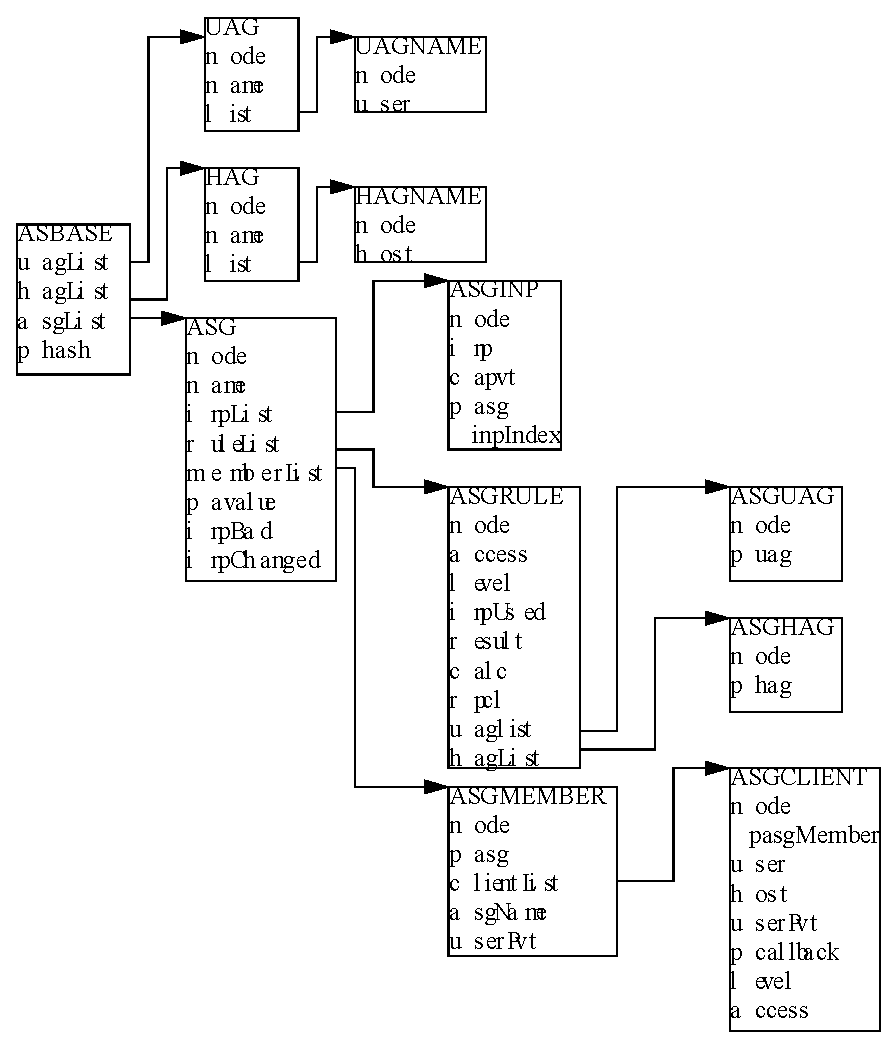
\includegraphics{accessSecurity_1}
\end{center}

\chapter{IOC Test Facilities}

\section{Overview}

This chapter describes a number of IOC test routines that are of interest to both application developers and system 
developers. The routines are available from either iocsh or the vxWorks shell. In both shells the parentheses around 
arguments are optional. On vxWorks all character string arguments must be enclosed in double quote characters \verb|""| and 
all arguments must be separated by commas. For \index{iocsh}iocsh single or double quotes must be used around string arguments that 
contain spaces or commas but are otherwise optional, and arguments may be separated by either commas or spaces. For 
example:

\begin{verbatim}
dbpf("aiTest","2")
dbpf "aiTest","2"
\end{verbatim}

are both valid with both iocsh and with the vxWorks shell.

\begin{verbatim}
dbpf aiTest 2
\end{verbatim}

Is valid for iocsh but not for the vxWorks shell.

Both iosch and vxWorks shells allow output redirection, i.e. the standard output of any command can be redirected to a 
file. For example

\begin{verbatim}
dbl > dbl.lst
\end{verbatim}

will send the output of the \verb|dbl| command to the file \verb|dbl.lst|

If iocsh is being used it provides help for all commands that have been registered. Just type

\begin{verbatim}
help
\end{verbatim}

or

\begin{verbatim}
help pattern*
\end{verbatim}

\section{Database List, Get, Put}

\subsection{dbl}

\index{dbl}
Database List:

\begin{verbatim}
dbl("<record type>","<field list>")
\end{verbatim}

Examples

\begin{verbatim}
dbl
dbl("ai")
dbl("*")
dbl("")

\end{verbatim}

This command prints the names of records in the run time database. If \verb|<record type>| is empty \verb|("")|, \verb|"*"|, or not 
specified, all records are listed. If \verb|<record type>| is specified, then only the names of the records of that type are 
listed.

If \verb|<field list>| is given and not empty then the values of the fields specified are also printed.

\subsection{dbgrep}

\index{dbgrep}
List Record Names That Match a Pattern:

\begin{verbatim}
dbgrep("<pattern>")
\end{verbatim}

Examples

\begin{verbatim}
dbgrep("S0*")
dbgrep("*gpibAi*")
\end{verbatim}

Lists all record names that match a pattern. The pattern can contain any characters that are legal in record names as well as 
"\verb|*|", which matches 0 or more characters.

\subsection{dbla}

\index{dbla}
List Record Alias Names with optional pattern:

\begin{verbatim}
dbla
dbla("<pattern>")
\end{verbatim}

Lists the names of all aliases (which match the pattern if given) and the records they refer to. Examples:

\begin{verbatim}
dbla
dbla "alia*"
\end{verbatim}

\subsection{dba}

\index{dba}
Database Address:

\begin{verbatim}
dba("<record_name.field_name>")
\end{verbatim}

Example

\begin{verbatim}
dba("aitest")
dba("aitest.VAL")
\end{verbatim}

This command calls \verb|dbNameToAddr| and then prints the value of each field in the \verb|dbAddr| structure describing the field. 
If the field name is not specified then \verb|VAL| is assumed (the two examples above are equivalent).

\subsection{dbgf}

\index{dbgf}
Get Field:

\begin{verbatim}
dbgf("<record_name.field_name>")
\end{verbatim}

Example:

\begin{verbatim}
dbgf("aitest")
dbgf)"aitest.VAL")
\end{verbatim}

This performs a \verb|dbNameToAddr| and then a \verb|dbGetField|. It prints the field type and value. If the field name is not 
specified then \verb|VAL| is assumed (the two examples above are equivalent). Note that \verb|dbGetField| locks the record lockset, 
so \verb|dbgf| will not work on a record with a stuck lockset; use \verb|dbpr| instead in this case.

\subsection{dbpf}

\index{dbpf}
Put Field:

\begin{verbatim}
dbpf("<record_name.field_name>","<value>")
\end{verbatim}

Example:

\begin{verbatim}
dbpf("aitest","5.0")
\end{verbatim}

This command performs a \verb|dbNameToAddr| followed by a \verb|dbPutField| and \verb|dbgf|. If \verb|<field_name>| is not specified 
\verb|VAL| is assumed. 

\subsection{dbpr}

\index{dbpr}
Print Record:

\begin{verbatim}
dbpr("<record_name>",<interest level>)
\end{verbatim}

Example

\begin{verbatim}
dbpr("aitest",2)
\end{verbatim}

This command prints all fields of the specified record up to and including those with the indicated interest level. Interest 
level has one of the following values:

\begin{itemize}
\item 0:  Fields of interest to an Application developer and that can be changed as a result of record processing.

\item 1:  Fields of interest to an Application developer and that do not change during record processing.

\item 2: Fields of major interest to a System developer.

\item 3: Fields of minor interest to a System developer.

\item 4: Fields of no interest.

\end{itemize}

\subsection{ dbtr}

\index{dbtr}
Test Record:

\begin{verbatim}
dbtr("<record_name>")
\end{verbatim}

This calls \verb|dbNameToAddr|, then \verb|dbProcess| and finally \verb|dbpr| (interest level 3). Its purpose is to test record processing.

\subsection{dbnr}

\index{dbnr}
Print number of records:

\begin{verbatim}
dbnr(<all_recordtypes>)
\end{verbatim}

This command displays the number of records of each type and the total number of records. If \verb|all_record_types| is 
0 then only record types with record instances are displayed otherwise all record types are displayed.

\section{Breakpoints}

\index{Breakpoints}
A breakpoint facility that allows the user to step through database processing on a per lockset basis. This facility has been 
constructed in such a way that the execution of all locksets other than ones with breakpoints will not be interrupted. This 
was done by executing the records in the context of a separate task.

The breakpoint facility records all attempts to process records in a lockset containing breakpoints. A record that is 
processed through external means, e.g.: a scan task, is called an entrypoint into that lockset. The \verb|dbstat| command 
described below will list all detected entrypoints to a lockset, and at what rate they have been detected.

\subsection{dbb}

\index{dbb}
Set Breakpoint:

\begin{verbatim}
dbb("<record_name>")
\end{verbatim}

Sets a breakpoint in a record. Automatically spawns the \verb|bkptCont|, or breakpoint continuation task (one per lockset). 
Further record execution in this lockset is run within this task's context. This task will automatically quit if two conditions 
are met, all breakpoints have been removed from records within the lockset, and all breakpoints within the lockset have 
been continued.

\subsection{dbd}

\index{dbd}
Remove Breakpoint:

\begin{verbatim}
dbd("<record_name>")
\end{verbatim}

Removes a breakpoint from a record.

\subsection{dbs}

\index{dbs}
Single Step:

\begin{verbatim}
dbs("<record_name>")
\end{verbatim}

Steps through execution of records within a lockset. If this command is called without an argument, it will automatically 
step starting with the last detected breakpoint.

\subsection{dbc}

\index{dbc}
Continue:

\begin{verbatim}
dbc("<record_name>")
\end{verbatim}

Continues execution until another breakpoint is found. This command may also be called without an argument.

\subsection{dbp }

\index{dbp}
Print Fields Of Suspended Record:

\begin{verbatim}
dbp("<record_name>,<interest_level>)
\end{verbatim}

Prints out the fields of the last record whose execution was suspended.

\subsection{dbap}

\index{dbap}
Auto Print:

\begin{verbatim}
dbap("<record_name>")
\end{verbatim}

Toggles the automatic record printing feature. If this feature is enabled for a given record, it will automatically be printed 
after the record is processed.

\subsection{dbstat}

\index{dbstat}
Status:

\begin{verbatim}
dbstat
\end{verbatim}

Prints out the status of all locksets that are suspended or contain breakpoints. This lists all the records with breakpoints 
set, what records have the autoprint feature set (by \verb|dbap|), and what entrypoints have been detected. It also displays the 
vxWorks task ID of the breakpoint continuation task for the lockset. Here is an example output from this call:

\begin{verbatim}
LSet: 00009  Stopped at: so#B: 00001   T: 0x23cafac
             Entrypoint: so#C: 00001   C/S:     0.1
             Breakpoint: so(ap)
LSet: 00008#B: 00001   T: 0x22fee4c
             Breakpoint: output
\end{verbatim}

The above indicates that two locksets contain breakpoints. One lockset is stopped at record ``\verb|so|." The other is not 
currently stopped, but contains a breakpoint at record ``\verb|output|." ``\verb|LSet:|" is the lockset number that is being considered. 
"\verb|#B:|" is the number of breakpoints set in records within that lockset. ``\verb|T:|" is the vxWorks task ID of the continuation 
task. ``\verb|C:|" is the total number of calls to the entrypoint that have been detected. ``\verb|C/S:|" is the number of those calls that 
have been detected per second. \verb|(ap)| indicates that the autoprint feature has been turned on for record ``\verb|so|."

\section{Trace Processing}

\index{Trace Processing}
The user should also be aware of the field \verb|TPRO|, which is present in every database record. If it is set \verb|TRUE| then a 
message is printed each time its record is processed and a message is printed for each record processed as a result of it 
being processed.

\index{TPRO}
\section{Error Logging}

\subsection{eltc}

\index{eltc}
Display error log messages on console:

\begin{verbatim}
eltc(int noYes)
\end{verbatim}

This determines if error messages are displayed on the IOC console. 0 means no and any other value means yes.

\subsection{errlogInit, errlogInit2}

Initialize error log client buffering

\begin{verbatim}
errlogInit(int bufSize)
errlogInit2(int bufSize, int maxMsgSize)
\end{verbatim}

The error log client maintains a circular buffer of messages that are waiting to be sent to the log server.  If not set using 
one or other of these routines the default value for bufSize is 1280 bytes and for maxMsgSize is 256 bytes.

\subsection{errlog}

Send a message to the log server

\begin{verbatim}
errlog("<message>")
\end{verbatim}

This command is provided for use from the ioc shell only.  It sends its string argument and a new-line to the log server, 
without displaying it on the IOC console. Note that the iocsh will have expanded any environment variable macros in the 
string (if it was double-quoted) before passing it to errlog.

\section{Hardware Reports}

\subsection{dbior}

\index{dbior}
I/O Report:

\begin{verbatim}
dbior ("<driver_name>",<interest level>)
\end{verbatim}

This command calls the report entry of the indicated driver. If \verb|<driver_name>| is ``" or ``*", then a report for all drivers 
is generated. The command also calls the report entry of all device support modules. Interest level is one of the following:

\begin{itemize}
\item 0: Print a short report for each module.

\item 1:  Print additional information.

\item 2:  Print even more info. The user may be prompted for options.

\end{itemize}

\subsection{dbhcr}

\index{dbhcr}
Hardware Configuration Report:

\begin{verbatim}
dbhcr()
\end{verbatim}

This command produces a report of all hardware links. To use it on the IOC, issue the command:

\begin{verbatim}
dbhcr > report
\end{verbatim}

The report will probably not be in the sort order desired. The Unix command:

\begin{verbatim}
sort report > report.sort
\end{verbatim}

should produce the sort order you desire.

\section{Scan Reports}

\subsection{scanppl}

\index{scanppl}
Print Periodic Lists:

\begin{verbatim}
scanppl(double rate)
\end{verbatim}

This routine prints a list of all records in the periodic scan list of the specified rate. If rate is 0.0 all period lists are shown.

\subsection{scanpel}

\index{scanpel}
Print Event Lists:

\begin{verbatim}
scanpel(int event_number)
\end{verbatim}

This routine prints a list of all records in the event scan list for the specified event nunber. If event\_number is 0 all event 
scan lists are shown.

\subsection{scanpiol}

\index{scanpiol}
Print I/O Event Lists:

\begin{verbatim}
scanpiol
\end{verbatim}

This routine prints a list of all records in the I/O event scan lists.

\section{General Time}

The built-in time providers depend on the IOC's target architecture, so some of the specific subsystem report commands 
listed below are only available on the architectures that use that particular provider.

\subsection{generalTimeReport}

\index{generalTimeReport}
Format:

\begin{verbatim}
generalTimeReport(int level)
\end{verbatim}

This routine displays the time providers and their priority levels that have registered with the General Time subsystem  for 
both current and event times. At level 1 it also shows the current time as obtained from each provider.

\subsection{installLastResortEventProvider}

\index{installLastResortEventProvider}
Format:

\begin{verbatim}
installLastResortEventProvider
\end{verbatim}

Installs the optional Last Resort event provider at priority 999, which returns the current time for every event number.

\subsection{NTPTime\_Report}

\index{NTPTime\_Report}
Format:

\begin{verbatim}
NTPTime_Report(int level)
\end{verbatim}

Only vxWorks and RTEMS targets use this time provider. The report displays the provider's synchronization state, and at 
interest level 1 it also gives the synchronization interval, when it last synchronized, the nominal and measured system tick 
rates, and on vxWorks the NTP server address.

\subsection{NTPTime\_Shutdown}

Format:

\begin{verbatim}
NTPTime_Shutdown
\end{verbatim}

On vxWorks and RTEMS this command shuts down the NTP time synchronization thread. With the thread shut down, the 
driver will no longer act as a current time provider.

\subsection{ClockTime\_Report}

\index{ClockTime\_Report}
Format:

\begin{verbatim}
ClockTime_Report(int level)
\end{verbatim}

This time provider is used on several target architectures, registered as the time provider of last resort. On vxWorks and 
RTEMS the report displays the synchronization state, when it last synchronized the system time with a higher priority 
provider, and the synchronization interval. On workstation operating systems the synchronization task is not started on the 
assumption that some other process is taking care of synchronzing the OS clock as appropriate, so the report is minimal.

\subsection{ClockTime\_Shutdown}

\index{ClockTime\_Shutdown}
Format:

\begin{verbatim}
ClockTime_Shutdown
\end{verbatim}

Some sites may prefer to provide their own implementation of a system clock time provider to replace the built-in one. On 
vxWorks and RTEMS this command stops the OS Clock synchronization thread, allowing the OS clock to free-run.  The 
time provider \emph{will} continue to return the current system time after this command is used however.

\section{Access Security Commands}

\subsection{asSetSubstitutions}

Format:

\begin{verbatim}
asSetSubstitutions("substitutions")
\end{verbatim}

Specifies macro substitutions used when access security is initialized.

\subsection{asSetFilename}

\index{asSetFilename}
Format:

\begin{verbatim}
asSetFilename("<filename>")
\end{verbatim}

This command defines a new access security file.

\subsection{asInit}

\index{asInit}
Format:

\begin{verbatim}
asInit
\end{verbatim}

This command reinitializes the access security system.  It rereads the access security file in order to create the new access 
security database. This command is useful either because the \verb|asSetFilename| command was used to change the file or 
because the file itself was modified.  Note that it is also possible to reinitialize the access security via a subroutine record.  
See the access security document for details.

\subsection{asdbdump}

\index{asdbdump}
Format:

\begin{verbatim}
asdbdump
\end{verbatim}

This provides a complete dump of the access security database.

\subsection{aspuag}

\index{aspuag}
Format:

\begin{verbatim}
aspuag("<user access group>")
\end{verbatim}

Print the members of the user access group.  If no user access group is specified then the members of all user access 
groups are displayed.

\subsection{asphag}

\index{asphag}
Format:

\begin{verbatim}
asphag("<host access group>")
\end{verbatim}

Print the members of the host access group.  If no host access group is specified then the members of all host access 
groups are displayed.

\subsection{asprules}

\index{asprules}
Format:

\begin{verbatim}
asprules("<access security group>")
\end{verbatim}

Print the rules for the specified access security group or if no group is specified for all groups.

\subsection{aspmem}

\index{aspmem}
Format:

\begin{verbatim}
aspmem("<access security group>", <print clients>)
\end{verbatim}

Print the members (records) that belong to the specified access security group, for all groups if no group is specified.  If 
\verb|<print clients>| is (0, 1) then Channel Access clients attached to each member (are not, are) shown.

\section{Channel Access Reports}

\subsection{casr}

\index{casr}
Channel Access Server Report

\begin{verbatim}
casr(<level>)
\end{verbatim}

Level can have one of the following values:

\begin{description}

\item 0 

Prints server's protocol version level and a one line summary for each client attached. The summary lines 
contain the client's login name, client's host name, client's protocol version number, and the number of 
channel created within the server by the client.

\item 1

Level one provides all information in level 0 and adds the task id used by the server for each client, the 
client's IP protocol type, the file number used by the server for the client, the number of seconds elapsed 
since the last request was received from the client, the number of seconds elapsed since the last response 
was sent to the client, the number of unprocessed request bytes from the client, the number of response bytes 
which have not been flushed to the client, the client's IP address, the client's port number, and the client's 
state.

\item 2

Level two provides all information in levels 0 and 1 and adds the number of bytes allocated by each client 
and a list of channel names used by each client. Level 2 also provides information about the number of bytes 
in the server's free memory pool, the distribution of entries in the server's resource hash table, and the list of 
IP addresses to which the server is sending beacons. The channel names are shown in the form:

\textless{}name\textgreater{}(nrw)

where

\begin{description}
\item n is number of ca\_add\_events the client has on this channel
\item r is (-,R) if client (does not, does) have read access to the channel.
\item w is(-, W) if client (does not, does) have write access to the channel.
\end{description}

\end{description}

\subsection{dbel}

\index{dbel}
Format:

\begin{verbatim}
dbel("<record_name>")
\end{verbatim}

This routine prints the Channel Access event list for the specified record.

\subsection{dbcar}

\index{dbcar}
Database to Channel Access Report - See ``Record Link Reports"

\subsection{ascar}

\index{ascar}
Format:

\begin{verbatim}
ascar(level)
\end{verbatim}

Prints a report of the channel access links for the INP fields of the access security rules. Level 0 produces a summary 
report. Level 1 produces a summary report plus details on any unconnect channels. Level 2 produces the summary nreport 
plus a detail report on each channel.

\section{Interrupt Vectors}

\subsection{veclist}

\index{veclist}
Format:

\begin{verbatim}
veclist
\end{verbatim}

NOTE: This routine is only available on vxWorks. On PowerPC CPUs it requires BSP support to work, and even then it 
cannot display chained interrupts using the same vector.

Print Interrupt Vector List

\section{Miscellaneous}

\subsection{epicsParamShow}

\index{epicsParamShow}
Format:

\begin{verbatim}
epicsParamShow
or
epicsPrtEnvParams
\end{verbatim}

Print the environment variables that are created with epicsEnvSet. These are defined in \textless{}base\textgreater{}/config/CONFIG\_ENV 
and \textless{}base\textgreater{}/config/CONFIG\_SITE\_ENV or else by user applications calling \verb|epicsEnvSet|.

\subsection{epicsEnvShow}

\index{epicsEnvShow}
Format:

\begin{verbatim}
epicsEnvShow("<name>")
\end{verbatim}

Show Environment variables. On vxWorks it shows the variables created via calls to \verb|putenv|.

\subsection{coreRelease}

\index{coreRelease}
Format:

\begin{verbatim}
coreRelease
\end{verbatim}

Print release information for iocCore.

\section{Database System Test Routines}

These routines are normally only of interest to EPICS system developers NOT to Application Developers.

\subsection{dbtgf}

\index{dbtgf}
Test Get Field:

\begin{verbatim}
dbtgf("<record_name.field_name>")
\end{verbatim}

Example:

\begin{verbatim}
dbtgf("aitest")
dbtgf)"aitest.VAL")
\end{verbatim}

This performs a \verb|dbNameToAddr| and then calls \verb|dbGetField| with all possible request types and options. It prints the 
results of each call. This routine is of most interest to system developers for testing database access.

\subsection{dbtpf}

\index{dbtpf}
Test Put Field:

\begin{verbatim}
dbtpf("<record_name.field_name>","<value>")
\end{verbatim}

Example:

\begin{verbatim}
dbtpf("aitest","5.0")
\end{verbatim}

This command performs a \verb|dbNameToAddr|, then calls \verb|dbPutField|, followed by \verb|dbgf| for each possible request type. 
This routine is of interest to system developers for testing database access.

\subsection{dbtpn}

\index{dbtpn}
Test Process Notify:

\begin{verbatim}
dbtpn("<record_name.field_name>")
dbtpn("<record_name.field_name>","<value>")
\end{verbatim}

Example:

\begin{verbatim}
dbtpn("aitest")
dbtpn("aitest","5.0")
\end{verbatim}

This command performs a \verb|dbProcessNotify| request. If a value argument is provided it issues a \verb|putProcessRequest| to the named record; if no value is provided it issues a \verb|processGetRequest|. This routine is mainly of interest to system developers for testing database access.

\section{Record Link Reports}

\subsection{dblsr}

\index{dblsr}
Lock Set Report:

\begin{verbatim}
dblsr(<recordname>,<level>)
\end{verbatim}

This command generates a report showing the lock set to which each record belongs. If \verb|recordname| is 0, \verb|""|, or \verb|"*"| all 
records are shown, otherwise only records in the same lock set as \verb|recordname| are shown.

\verb|level| can have the following values:

\begin{description}
\item 0 - Show lock set information only.

\item 1 - Show each record in the lock set.

\item 2 - Show each record and all database links in the lock set.

\end{description}

\subsection{dbLockShowLocked}

\index{dbLockShowLocked}
Show locked locksets:

\begin{verbatim}
dbLockShowLocked(<level>)
\end{verbatim}

This command generates a report showing all locked locksets, the records they contain, the lockset state and the thread 
that currently owns the lockset. The \verb|level| argument is passed to \verb|epicsMutexShow| to adjust the information reported 
about each locked epicsMutex.

\subsection{dbcar}

\index{dbcar}
Database to channel access report

\begin{verbatim}
dbcar(<recordname>,<level>)
\end{verbatim}

This command generates a report showing database channel access links. If \verb|recordname| is ``*" then information about 
all records is shown otherwise only information about the specified record.

\verb|level| can have the following values:

\begin{description}
\item 0 - Show summary information only.

\item 1 - Show summary and each CA link that is not connected.

\item 2 - Show summary and status of each CA link.

\end{description}

\subsection{dbhcr}

\index{dbhcr}
Report hardware links. See ``Hardware Reports".

\section{Old Database Access Testing}

These routines are of interest to EPICS system developers. They are used to test the old database access interface, which 
is still used by Channel Access.

\subsection{gft}

\index{gft}
Get Field Test:

\begin{verbatim}
gft("<record_name.field_name>")
\end{verbatim}

Example:

\begin{verbatim}
gft("aitest")
gft("aitest.VAL")
\end{verbatim}

This performs a \verb|db_name_to_addr| and then calls \verb|db_get_field| with all possible request types. It prints the results 
of each call. This routine is of interest to system developers for testing database access.

\subsection{pft}

\index{pft}
Put Field Test:

\begin{verbatim}
pft("<record_name.field_name>","<value>")
\end{verbatim}

Example:

\begin{verbatim}
pft("aitest","5.0")
\end{verbatim}

This command performs a \verb|db_name_to_addr|, \verb|db_put_field|, \verb|db_get_field| and prints the result for each 
possible request type. This routine is of interest to system developers for testing database access.

\subsection{tpn}

\index{tpn}
Test Process Notify:

\begin{verbatim}
tpn("<record_name.field_name>","<value>")
\end{verbatim}

Example:

\begin{verbatim}
tpn("aitest","5.0")
\end{verbatim}

This routine tests \verb|dbProcessNotify| via the old database access interface.
It only supports issuing a \verb|putProcessRequest| to the named record.

\section{Routines to dump database information}

\subsection{dbDumpPath}

\index{dbDumpMenu}
Dump Path:

\begin{verbatim}
dbDumpPath(pdbbase)
\end{verbatim}

\begin{verbatim}
   dbDumpPath(pdbbase)
\end{verbatim}

The current path for database includes is displayed.

\subsection{dbDumpMenu}

\index{dbDumpMenu}
Dump Menu:

\begin{verbatim}
dbDumpMenu(pdbbase,"<menu>")
\end{verbatim}

\begin{verbatim}
   dbDumpMenu(pdbbase,"menuScan")
\end{verbatim}

If the second argument is 0 then all menus are displayed.



\subsection{dbDumpRecordType}

\index{dbDumpRecordType}
Dump Record Description:

\begin{verbatim}
dbDumpRecordType(pdbbase,"<record type>")
\end{verbatim}

\begin{verbatim}
   dbDumpRecordType(pdbbase,"ai")
\end{verbatim}

If the second argument is 0 then all descriptions of all records are displayed.

\subsection{dbDumpField}

\index{dbDumpField}
Dump Field Description:

\begin{verbatim}
dbDumpField(pdbbase,"<record type>","<field name>")
\end{verbatim}

\begin{verbatim}
   dbDumpField(pdbbase,"ai","VAL")
\end{verbatim}

If the second argument is 0 then the field descriptions of all records are displayed. If the third argument is 0 then the 
description of all fields are displayed.

\subsection{dbDumpDevice}

\index{dbDumpDevice}
Dump Device Support:

\begin{verbatim}
dbDumpDevice(pdbbase,"<record type>")
\end{verbatim}

\begin{verbatim}
   dbDumpDevice(pdbbase,"ai")
\end{verbatim}

If the second argument is 0 then the device support for all record types is displayed.

\subsection{dbDumpDriver}

\index{dbDumpDriver}
Dump Driver Support:

\begin{verbatim}
dbDumpDriver(pdbbase)
\end{verbatim}

\begin{verbatim}
   dbDumpDriver(pdbbase)
\end{verbatim}

\subsection{dbDumpRecord}

\index{dbDumpRecords}
Dump Record Instances:

\begin{verbatim}
dbDumpRecord(pdbbase,"<record type>",level)
\end{verbatim}

\begin{verbatim}
   dbDumpRecords(pdbbase,"ai")
\end{verbatim}

If the second argument is 0 then the record instances for all record types are displayed. The third argument determines 
which fields are displayed just like for the command \verb|dbpr|.

\subsection{dbDumpBreaktable}

Dump breakpoint table

\begin{verbatim}
dbDumpBreaktable(pdbbase,name)
\end{verbatim}

\begin{verbatim}
   dbDumpBreaktable(pdbbase,"typeKdegF")
\end{verbatim}

This command dumps a breakpoint table. If the second argument is 0 all breakpoint tables are dumped.

\subsection{dbPvdDump}

\index{dbPvdDump}
Dump the Process variable Directory:

\begin{verbatim}
dbPvdDump(pdbbase,verbose)
\end{verbatim}

\begin{verbatim}
   dbPvdDump(pdbbase,0)
\end{verbatim}

This command shows how many records are mapped to each hash table entry of the process variable directory. If verbose 
is not 0 then the command also displays the names which hash to each hash table entry.


\chapter{IOC Error Logging}
\index{IOC Error Logging}

\section{Overview }

Errors detected by an IOC can be divided into classes: Errors related to a particular client and errors not attributable to a 
particular client. An example of the first type of error is an illegal Channel Access request. For this type of error, a status 
value should be passed back to the client. An example of the second type of error is a device driver detecting a hardware 
error. This type of error should be reported to a system wide error handler.

Dividing errors into these two classes is complicated by a number of factors.

\begin{itemize}\item In many cases it is not possible for the routine detecting an error to decide which type of error occurred. 

\item Normally, only the routine detecting the error knows how to generate a fully descriptive error message. Thus, if a 
routine decides that the error belongs to a particular client and merely returns an error status value, the ability to 
generate a fully descriptive error message is lost. 

\item If a routine always generates fully descriptive error messages then a particular client could cause error message 
storms.

\item While developing a new application the programmer normally prefers fully descriptive error messages. For a 
production system, however, the system wide error handler should not normally receive error messages cause by a 
particular client.

\end{itemize}If used properly, the error handling facilities described in this chapter can process both types of errors.

This chapter describes the following:

\begin{itemize}\item Error Message Generation Routines - Routines which pass messages to the errlog Task.

\item Error Log Listeners - Any code can register to recieve errlog messages.

\item errlogThread - A thread that passes the messages to all registered listeners.

\item console output and message buffer size - Messages can also be written to the console. The storage for the message 
queue can be specified by the user.

\item status codes - EPICS status codes.

\item iocLog- A system wide error logger supplied with base. It writes all messages to a system wide file.

NOTE: Many sites use CMLOG instead of iocLog.

\end{itemize}NOTE: \verb|recGbl| error routines are also provided. They in turn call one of the error message routines.

\section{Error Message Routines}

\subsection{Basic Routines}

\begin{verbatim}
   int errlogPrintf(const char *pformat, ...);
   int errlogVprintf(const char *pformat,va_list pvar);
   int errlogMessage(const char *message);
   void errlogFlush(void);
\end{verbatim}
\index{errlogPrintf}
\index{errlogVprintf}
\index{errlogMessage}
\index{errlogFlush} \verb|errlogPrintf |and  \verb|errlogVprintf| are like \verb|printf| and \verb|vprintf| provided by the standard C library, except 
that their output is sent to the errlog task; unless configured not to, the output will appear on the console as well. Consult 
any book that describes the standard C library such as ``The C Programming Language ANSI C Edition" by Kernighan 
and Ritchie.

\verb|errlogMessage| sends message to the errlog task.

\verb|errlogFlush| wakes up the errlog task and then waits until all messages are flushed from the queue.

\subsection{Log with Severity}

\begin{verbatim}
typedef enum {
    errlogInfo,errlogMinor,errlogMajor,errlogFatal
}errlogSevEnum;

int errlogSevPrintf(const errlogSevEnum severity,
    const char *pformat, ...);
int errlogSevVprintf(const errlogSevEnum severity,
    const char *pformat,va_list pvar);

char *errlogGetSevEnumString(const errlogSevEnum severity);

void  errlogSetSevToLog(const errlogSevEnum severity );
errlogSevEnum errlogGetSevToLog(void);
\end{verbatim}\index{errlogInfo}
\index{errlogMinor}
\index{errlogMajor}
\index{errlogFatal}
\index{errlogSevEnum}
\index{errlogSevPrintf}
\index{errlogSevVprintf}
\index{errlogGetSevEnumString}
\index{errlogSetSevToLog}
\index{errlogGetSevToLog}\verb|errlogSevPrintf| and \verb|errlogSevVprintf| are like \verb|errlogPrintf |and  \verb|errlogVprintf| except that they 
add the severity to the beginning of the message in the form ``sevr=\textless{}value\textgreater{}" where value is on of ``info, minor, major, 
fatal". Also the message is suppressed if  severity is less than the current severity to suppress. If epicsThreadIsOkToBlock 
is true, which is true during iocInit, errlogSevVprintf does NOT send output to the errlog task.

\verb|errlogGetSevEnumString| gets the string value of severity. 

 \verb|errlogSetSevToLog| sets the severity to log. \verb|errlogGetSevToLog| gets the current severity to log.

\subsection{Status Routines }

\begin{verbatim}
void errMessage(long status, char *message);

void errPrintf(long status, const char *pFileName,
    int lineno, const char *pformat, ...);
\end{verbatim}\index{errMessage}
\index{errPrintf}Routine \verb|errMessage| (actually a macro that calls \verb|errPrintf|) has the following format:

\index{errMessage}\begin{verbatim}void errMessage(long  status, char  *message);
\end{verbatim}Where status is defined as:

\begin{itemize}\item 0:  Find latest vxWorks or Unix error.

\item -1:  Don't report status.

\item Other:  See ``Return Status Values" above.

\end{itemize}\verb|errMessage|, via a call to \verb|errPrintf|, prints the message, the status symbol and string values, and the name of the task 
which invoked \verb|errMessage|. It also prints the name of the source file and the line number from which the call was 
issued.

The calling routine is expected to pass a descriptive message to this routine. Many subsystems provide routines built on 
top of \verb|errMessage| which generate descriptive messages. 

An IOC global variable \verb|errVerbose|, defined as an \verb|external| in \verb|errMdef.h|, specifies verbose messages. If 
\verb|errVerbose| is \verb|TRUE| then \verb|errMessage| should be called whenever an error is detected even if it is known that the 
error belongs to a specific client. If \verb|errVerbose| is \verb|FALSE| then \verb|errMessage| should be called only for errors that are 
not caused by a specific client.

Routine \verb|errPrintf| is normally called as follows:

\index{errPrintf}\begin{verbatim}errPrintf(status, __FILE__, __LINE__,"<fmt>",...);
\end{verbatim}Where status is defined as:

\begin{itemize}\item 0:  Find latest vxWorks or Unix error.

\item -1:  Don't report status.

\item Other:  See ``Return Status Values", above.

\end{itemize}FILE and LINE are defined as:

\begin{itemize}\item \_\_FILE\_\_   As shown or \verb|NULL| if the file name and line number should not be printed.

\item \_\_LINE\_\_  As shown

\end{itemize}The remaining arguments are just like the arguments to the C \verb|printf| routine. \verb|errVerbose| determines if the filename 
and line number are shown.

An EPICS status code can also be converted to a string. If the supplied status code isn't registered in the status code 
database then the raw status code number is converted into a string in the destination buffer.

\begin{verbatim}#include "errMdef.h"
void errSymLookup(long status, char *pBuf, unsigned bufLength);
\end{verbatim}\subsection{Obsolete Routines }

\begin{verbatim}int epicsPrintf(const char *pformat, ...);
int epicsVprintf(const char *pformat,va_list pvar);
\end{verbatim}\index{epicsPrintf}
\index{epicsVprintf}These are macros that call errlogPrintf and errlogVprintf. They are provided for compatibility.

\section{errlog Listeners}

\index{errlog Listeners}Any code can receive errlog message. The following are the calls to add and remove a listener.

\begin{verbatim}
typedef void(*errlogListener) (void *pvt,const char *message);
void errlogAddListener(errlogListener listener,void *pPrivate);
void errlogRemoveListener(errlogListener listener);
\end{verbatim}\index{errlogListener}
\index{errlogAddListener}
\index{errlogRemoveListener}These routines add/remove a callback that receives each error message. These routines are the interface to the actual 
system wide error handlers.

\section{errlogThread}

\index{errlogThread}The error message routines can be called by any non-interrupt level code. These routines pass the message to the errlog 
Thread. If any of the error message routines are called at interrupt level,  \verb|epicsInterruptContextMessage| is 
called with the message ``errlogPrintf called from interrupt level".

errlogThread manages the messages. Messages are placed in a message queue, which is read by errlogThread. The 
message queue uses a fixed block of memory to hold all messages. When the message queue is full additional messages 
are rejected but a count of missed messages is kept. The next time the message queue empties an extra message about the 
missed messages is generated.

The maximum message size is by default 256  characters. If a message is longer, the message is truncated and a message 
explaining that it was truncated is appended. There is a chance that long messages corrupt memory. This  only happens if 
client code is defective. Long messages most likely result from ``\%s" formats with a bad string argument.

errlogThread passes each message to any registered listener.

\section{console output and message queue size}

The errlog system can also display messages on the ioc console. It calls \verb|epicsThreadIsOkToBlock| to decide when 
to display the message. If it is OK to block, the message is displayed by the same thread that calls one of the errlog print 
routines. If it is not OK to block, errlorThread displays the messages.

Normally the errlog system displays all messages on the console. \verb|eltc| can be used to suppress these messages.

\begin{verbatim}int eltc(int yesno); /* error log to console (0 or 1) */
int errlogInit(int bufsize);
int errlogInit2(int bufsize, int maxMsgSize);
\end{verbatim}\index{eltc}
\index{errlogInit}
\index{errlogInit2}eltc determines if errlog task writes message to the console. During error messages storms  this  command can be used to 
suppress console messages. A argument of 0 suppresses the messages and any other value lets the message go to the 
console. 

errlogInit or errlogInit2 can be used to initialize the error logging system with a larger buffer and maximum message size. 
The default buffer size is 1280 bytes, and the default maximum message size is 256.

\section{Status Codes}

\index{status codes}EPICS defined status values provide the following features:

\begin{itemize}\item Whenever possible, IOC routines return a status value: (0, non-0) means (\verb|OK|, \verb|ERROR|).

\item The include files for each IOC subsystem contain macros defining error status symbols and strings.

\item Routines are provided for run time access of the error status symbols and strings.

\item A global variable \verb|errVerbose| helps code decide if error messages should be generated.

\end{itemize}WARNING: During the fall of 1995 a series of tech-talk messages were generated concerning EPICS status values. No 
consensus was reached.

Whenever it makes sense, IOC routines return a status value encoded similar to the vxWorks error status encoding. The 
most significant short word indicates the subsystem module within which the error occurred. The low order short word is 
a subsystem status value. In order that status values do not conflict with the vxWorks error status values all subsystem 
numbers are greater than 500. 

A file \verb|epics/share/epicsH/errMdef.h| defines each subsystem number. For example the \verb|define| for the 
database access routines is:

\begin{verbatim}#define M_dbAccess  (501 << 16)   \
/*Database Access Routines*/
\end{verbatim}Directory ``\verb|epics/share/epicsH|" contains an \verb|include| library for every IOC subsystem that returns standard status 
values. The status values are encoded with lines of the following format: 

\begin{verbatim}#define S_xxxxxxx value /*string value*/
\end{verbatim}For example:

\begin{verbatim}#define S_dbAccessBadDBR (M_dbAccess|3) \
/*Invalid Database Request*/
\end{verbatim}For example, when \verb|dbGetField| detects a bad database request type, it executes the statement:

\begin{verbatim}return(S_dbAccessBadDBR);
\end{verbatim}The calling routine checks the return status as follows:

\begin{verbatim}status = dbGetField( ...);
if(status) {/* Call was not successful */ }
\end{verbatim}\section{iocLog}

\index{iocLog}NOTE: Many sites use CMLOG instead of iocLog. See the CMLOG documentation for details.

This consists of two modules: iocLogServer and iocLogClient. The client code runs on each ioc and listens for the 
messages generated locally by the errlog system. It also reports the messages from the vxWorks logMsg facility.

\subsection{iocLogServer}

\index{iocLogServer}This runs on a host. It receives messages for all enabled iocLogClients in the local area network. The messages are written 
to a file. Epics base provides a startup file ``base/src/util/rc2.logServer", which is a SystemV init script to start the server. 
Consult this script for details.

To start a log server on a UNIX or PC workstation you must first set the following environment variables and then run the 
executable ``iocLogServer" on your PC or UNIX workstation. 

\begin{description}

\item \index{EPICS\_IOC\_LOG\_FILE\_NAME}EPICS\_IOC\_LOG\_FILE\_NAME 

The name and path to the log file.

\item \index{EPICS\_IOC\_LOG\_FILE\_LIMIT}EPICS\_IOC\_LOG\_FILE\_LIMIT

The maximum size in characters for the log file (after which it becomes a circular file and writes new 
messages over old  messages at the beginning of the file). If the value is zero then there is no limit on the 
size of the log file. 

\item \index{EPICS\_IOC\_LOG\_FILE\_COMMAND}EPICS\_IOC\_LOG\_FILE\_COMMAND

A shell command string used to obtain the log file path name during initialization and in response to 
SIGHUP. The new path name will replace any path name supplied in EPICS\_IOC\_LOG\_FILE\_NAME.

Thus, if EPICS\_IOC\_LOG\_FILE\_NAME is 

"a/b/c.log" and EPICS\_IOC\_LOG\_FILE\_COMMAND returns ``A/B" or ``A/B/" the log server will be stored 
at ``A/B/c.log"

If EPICS\_IOC\_LOG\_FILE\_COMMAND is empty then this behavior is disabled. This feature is used at 
some sites for switching the server to a new directory at a fixed time each day. This variable is currently 
used only by the UNIX version of the log server.

\item \index{EPICS\_IOC\_LOG\_PORT}EPICS\_IOC\_LOG\_PORT

THE TCP/IP port used by the log server.

\end{description}

To configure an IOC so that its messages are placed in the log you must set the environment variable 
EPICS\_IOC\_LOG\_INET to the IP address of the host that is running the log server, and EPICS\_IOC\_LOG\_PORT to the 
TCP/IP port used by the log server.

Defaults for all of the above parameters are specified in  the files \$(EPICS\_BASE)/config/CONFIG\_SITE\_ENV and 
\$(EPICS\_BASE)/config/CONFIG\_ENV.

\subsection{iocLogClient}

\index{iocLogClient}
This runs on each ioc. It is started by calling:

\begin{verbatim}iocLogInit();
\end{verbatim}The global variable \verb|iocLogDisable| can be used to enable/disable the messages from being sent to the server. Setting 
this variable to (0,1) (enables,disables) the messages generation. If \verb|iocLogDisable| is set to 1 before calling 
\verb|iocLogInit| then \verb|iocLogClient| will not even initialize itself. \verb|iocLogDisable| can also be changed to turn 
logging on or off.

\verb|iocLogClient| calls \verb|errlogAddListener| and sends each message to the \verb|iocLogServer|.

\subsection{Configuring a Private Log Server}

In a testing environment it is desirable to use a private log server. This can be done as follows:

\begin{itemize}

\item Add a epicsEnvSet command to your IOC startup file. For example

\begin{verbatim}ld  <  iocCore
epicsEnvSet("EPICS_IOC_LOG_INET=xxx.xxx.xxx.xxx")
\end{verbatim}

\item The inet address is that of your host workstation.

\item On your host workstation, start the log server.

\end{itemize}

\chapter{Record Support}
\index{Record Support}

\section{Overview}

The purpose of this chapter is to describe record support in sufficient detail such that a C programmer can write new record support modules.
Before attempting to write new support modules, you should carefully study a few of the existing support modules.
If an existing support module is similar to the desired module most of the work will already be done.

From previous chapters, it should be clear that many things happen as a result of record processing.
The details of what happens are dependent on the record type.
In order to allow new record types and new device types without impacting the core IOC system, the concept of record support and device support is used.
For each record type, a record support module exists.
It is responsible for all record specific details.
In order to allow a record support module to be independent of device specific details, the concept of device support has been created.

A record support module consists of a standard set of routines which are called by database access routines.
These routines implement record specific code.
Each record type can define a standard set of device support routines specific to that record type.

By far the most important record support routine is \verb|process|, which \verb|dbProcess| calls when it wants to process a record.
This routine is responsible for the details of record processing.
In many cases it calls a device support I/O routine.
The next section gives an overview of what must be done in order to process a record.
Next is a description of the entry tables that must be provided by record and device support modules.
The remaining sections give example record and device support modules and describe some global routines useful to record support modules.

The record and its device support modules are the only source files that should include the record specific header files.
Thus they will be the only routines that access record specific fields without going through database access.

\section{Overview of Record Processing}

\index{Overview of Record Processing}
The most important record support routine is \verb|process|.
This routine determines what record processing means.
Before the record specific ``\verb|process|" routine is called, the following has already been done:

\begin{itemize}
\item Decision to process a record.

\item Check that record is not active, i.e. \verb|pact| must be FALSE.

\item Check that the record is not disabled.

\end{itemize}

The \verb|process| routine, together with its associated device support, is responsible for the following tasks:

\begin{itemize}
\item Set record active while it is being processed

\item Perform I/O (with aid of device support)

\item Check for record specific alarm conditions

\item Raise database monitors

\item Request processing of forward links

\end{itemize}

A complication of record processing is that some devices are intrinsically asynchronous.
It is NEVER permissible to wait for a slow device to complete.
Asynchronous records perform the following steps:

\begin{enumerate}
\item Initiate the I/O operation and set \verb|pact = TRUE|

\item Determine a method for again calling process when the operation completes

\item Return immediately without completing record processing

\item When process is called after the I/O operation complete record processing

\item Set \verb|pact = FALSE| and return

\end{enumerate}

The examples given below show how this can be done.

\section{Record Support and Device Support Entry Tables}

Each record type has an associated set of record support routines.
These routines are located via the \verb|struct rset| data structure declared in \verb|recSup.h| and defined by the specific record type.
This use of a record support vector table isolates the \verb|iocCore| software from the implementation details of each record type.
Thus new record types can be defined without having to modify the IOC core software.

Each record type also has zero or more sets of device support routines.
Record types without associated hardware, e.g. calculation records, normally do not have any associated device support.
Record types with associated hardware normally have a  device support module for each device type.
The concept of device support isolates IOC core software and even record support from device specific details.

Corresponding to each record type is a set of record support routines.
The set of routines is the same for every record type.
These routines are located via a Record Support Entry Table (\index{RSET}\index{Record Support Entry Table}RSET), which has the following structure:

\begin{lstlisting}[language=C]
struct rset {   /* record support entry table */
    long     number;            /* number of support routine */
    RECSUPFUN   report;         /* print report */
    RECSUPFUN   init;           /* init support */
    RECSUPFUN   init_record;    /* init record */
    RECSUPFUN   process;        /* process record */
    RECSUPFUN   special;        /* special processing */
    RECSUPFUN   get_value;      /* OBSOLETE: Just leave NULL */
    RECSUPFUN   cvt_dbaddr;     /* cvt  dbAddr */
    RECSUPFUN   get_array_info;
    RECSUPFUN   put_array_info;
    RECSUPFUN   get_units;
    RECSUPFUN   get_precision;
    RECSUPFUN   get_enum_str;   /* get string from enum */
    RECSUPFUN   get_enum_strs;  /* get all enum strings */
    RECSUPFUN   put_enum_str;   /* put enum from string */
    RECSUPFUN   get_graphic_double;
    RECSUPFUN   get_control_double;
    RECSUPFUN   get_alarm_double;
};
\end{lstlisting}

Each record support module must define its RSET. The external name must be of the form:

\begin{verbatim}
<record_type>RSET
\end{verbatim}

Any routines not needed for the particular record type should be initialized to the value \verb|NULL|.
Look at the example below for details.

Device support routines are located via a Device Support Entry Table (\index{DSET}\index{Device Support Entry Table}DSET), which has the following structure:

\begin{lstlisting}[language=C]
struct dset {   /* device support entry table */
    long        number;     /* number of support routines */
    DEVSUPFUN   report;     /* print report */
    DEVSUPFUN   init;       /* init support */
    DEVSUPFUN   init_record;/* init record instance*/
    DEVSUPFUN    get_ioint_info;   /* get io interrupt info*/
    /* other functions are record dependent*/
};
\end{lstlisting}

Each device support module must define its associated DSET.
The external name must be the same as the name which appears in \verb|devSup.ascii|.

Any record support module which has associated device support must also include definitions for accessing its associated device support modules.
The field \verb|dset|, which is declared in \verb|dbCommon|, contains the address of the DSET.
It is given a value by \verb|iocInit|.

\section{Example Record Support Module}

This section contains the skeleton of a record support package.
The record type is \verb|xxx| and the record has the following fields in addition to the \verb|dbCommon| fields:
\verb|VAL|, \verb|PREC|, \verb|EGU|, \verb|HOPR|, \verb|LOPR|, \verb|HIHI|, \verb|LOLO|, \verb|HIGH|, \verb|LOW|, \verb|HHSV|, \verb|LLSV|, \verb|HSV|, \verb|LSV|, \verb|HYST|, \verb|ADEL|, \verb|MDEL|, \verb|LALM|, \verb|ALST|, \verb|MLST|.
These fields will have the same meaning as they have for the \verb|ai| record.
Consult the Record Reference manual for a description.

\subsection{Declarations}

\begin{lstlisting}[language=C]
/* Create RSET - Record Support Entry Table*/
#define report NULL
#define initialize NULL
static long init_record();
static long process();
#define special NULL
#define get_value NULL
#define cvt_dbaddr NULL
#define get_array_info NULL
#define put_array_info NULL
static long get_units();
static long get_precision();
#define get_enum_str NULL
#define get_enum_strs NULL
#define put_enum_str NULL
static long get_graphic_double();
static long get_control_double();
static long get_alarm_double();

rset xxxRSET={
    RSETNUMBER,
    report,
    initialize,
    init_record,
    process,
    special,
    get_value,
    cvt_dbaddr,
    get_array_info,
    put_array_info,
    get_units,
    get_precision,
    get_enum_str,
    get_enum_strs,
    put_enum_str,
    get_graphic_double,
    get_control_double,
    get_alarm_double
};
epicsExportAddress(rset,xxxRSET);

/* declarations for associated DSET */
typedef struct xxxdset { /* analog input dset */
    long   number;
    DEVSUPFUN   dev_report;
    DEVSUPFUN   init;
    DEVSUPFUN   init_record; /* returns: (1,0)=> (failure, success)*/
    DEVSUPFUN   get_ioint_info;
    DEVSUPFUN   read_xxx;
}xxxdset;

/* forward declaration for internal routines*/
static void checkAlarams(xxxRecord *pxxx);
static void monitor(xxxRecord *pxxx);
\end{lstlisting}

\index{RSET - example}The above declarations define the Record Support Entry Table (RSET), a template for the associated Device Support Entry Table (DSET), and forward declarations to private routines.

The RSET must be declared with an external name of \verb|xxxRSET|. It defines the record support routines supplied for this record type.
Note that forward declarations are given for all routines supported and a \verb|NULL| declaration for any routine not supported.

The template for the DSET is declared for use by this module.

\subsection{init\_record}

\index{init\_record - example}
\begin{lstlisting}[language=C]
static long init_record(void *precord, int  pass)
{
    xxxRecord*pxxx = (xxxRecord *)precord;
    xxxdset*pdset;
    longstatus;

    if(pass==0) return(0); 

    if((pdset = (xxxdset *)(pxxx->dset)) == NULL) {
        recGblRecordError(S_dev_noDSET,pxxx,"xxx: init_record");
        return(S_dev_noDSET);
    }
    /* must have read_xxx function defined */
    if( (pdset->number < 5) || (pdset->read_xxx == NULL) ) {
        recGblRecordError(S_dev_missingSup,pxxx,
        "xxx: init_record");
        return(S_dev_missingSup);
    }
    if( pdset->init_record ) {
        if((status=(*pdset->init_record)(pxxx))) return(status);
    }
    return(0);
}
\end{lstlisting}

This routine, which is called by \verb|iocInit| twice for each record of type \verb|xxx|, checks to see if it has a proper set of device support routines and, if present, calls the \verb|init_record| entry of the DSET.

During the first call to \verb|init_record| (pass=0) only initializations relating to this record can be performed.
During the second call (pass=1) initializations that may refer to other records can be performed.
Note also that during the second pass, other records may refer to fields within this record.
A good example of where these rules are important is a waveform record.
The \verb|VAL| field of a waveform record actually refers to an array.
The waveform record support module must allocate storage for the array.
If another record has a database link referring to the waveform \verb|VAL| field then the storage must be allocated before the link is resolved.
This is accomplished by having the waveform record support allocate the array during the first pass (pass=0) and having the link reference resolved during the second pass (pass=1).

\subsection{process}

\index{process - example}
\begin{lstlisting}[language=C]
static long process(void *precord)
{
    xxxRecord*pxxx = (xxxRecord *)precord;
        xxxdset*pdset = (xxxdset *)pxxx->dset;
    longstatus;
    unsigned char pact=pxxx->pact;

    if( (pdset==NULL) || (pdset->read_xxx==NULL) ) {
        /* leave pact true so that dbProcess doesnt call again*/
        pxxx->pact=TRUE;
        recGblRecordError(S_dev_missingSup,pxxx,"read_xxx");
        return(S_dev_missingSup);
    }

    /* pact must not be set true until read_xxx completes*/
    status=(*pdset->read_xxx)(pxxx); /* read the new value */
     /* return if beginning of asynch processing*/
    if(!pact && pxxx->pact) return(0);
    pxxx->pact = TRUE;
    recGblGetTimeStamp(pxxx);

    /* check for alarms */
    alarm(pxxx);
    /* check event list */
    monitor(pxxx);
    /* process the forward scan link record */
    recGblFwdLink(pxxx);

    pxxx->pact=FALSE;
    return(status);
}
\end{lstlisting}

The record processing routines are the heart of the IOC software.
The record specific process routine is called by \verb|dbProcess| whenever it decides that a record should be processed.
Process decides what record processing really means.
The above is a good example of what should be done.
In addition to being called by \verb|dbProcess| the process routine may also be called by asynchronous record completion routines.

The above model supports both synchronous and asynchronous device support routines.
For example, if \verb|read_xxx| is an asynchronous routine, the following sequence of events will occur:

\begin{itemize}
\item \verb|process| is called with \verb|pact| \verb|FALSE|

\item \verb|read_xxx| is called.
Since \verb|pact| is \verb|FALSE| it starts I/O, arranges callback, and sets \verb|pact| \verb|TRUE|

\item \verb|read_xxx| returns

\item because \verb|pact| went from \verb|FALSE| to \verb|TRUE| process just returns

\item Any new call to \verb|dbProcess| is ignored because it finds \verb|pact| \verb|TRUE|

\item Sometime later the callback occurs and \verb|process| is called again.

\item \verb|read_xxx| is called.
Since \verb|pact| is \verb|TRUE| it knows that it is a completion request.

\item \verb|read_xxx| returns

\item \verb|process| completes record processing

\item \verb|pact| is set \verb|FALSE|

\item \verb|process| returns

\end{itemize}

At this point the record has been completely processed.
The next time \verb|process| is called everything starts all over from the beginning.

\subsection{Miscellaneous Utility Routines}

\begin{lstlisting}[language=C]
static long get_units(DBADDR *paddr, char *units)
{
    xxxRecord  *pxxx=(xxxRecord *)paddr->precord;

    strncpy(units,pxxx->egu,sizeof(pxxx->egu));
    return(0);
}

static long get_graphic_double(DBADDR *paddr,
    struct dbr_grDouble *pgd)
{
    xxxRecord  *pxxx=(xxxRecord *)paddr->precord;
    int   fieldIndex = dbGetFieldIndex(paddr);

    if(fieldIndex == xxxRecordVAL) {
        pgd->upper_disp_limit = pxxx->hopr;
        pgd->lower_disp_limit = pxxx->lopr;
    } else recGblGetGraphicDouble(paddr,pgd);
    return(0);
}
/* similar routines would be provided for */
/* get_control_double and get_alarm_double*/
\end{lstlisting}

\index{get\_units - .example}
\index{get\_graphic\_double - example}
These are a few examples of various routines supplied by a typical record support package.
The functions that must be performed by the remaining routines are described in the next section.

\subsection{Alarm Processing}

\begin{lstlisting}[language=C]
static void checkAlarms(xxxRecord *prec)
{
	double		val;
	float		hyst, lalm, hihi, high, low, lolo;
	unsigned short	hhsv, llsv, hsv, lsv;

	if(prec->udf == TRUE ){
		recGblSetSevr(prec,UDF_ALARM,prec->udfs);
		return;
	}
	hihi = prec->hihi; lolo = prec->lolo; high = prec->high; low = prec->low;
	hhsv = prec->hhsv; llsv = prec->llsv; hsv = prec->hsv; lsv = prec->lsv;
	val = prec->val; hyst = prec->hyst; lalm = prec->lalm;

	/* alarm condition hihi */
	if (hhsv && (val >= hihi || ((lalm==hihi) && (val >= hihi-hyst)))){
	        if (recGblSetSevr(prec,HIHI_ALARM,prec->hhsv)) prec->lalm = hihi;
		return;
	}

	/* alarm condition lolo */
	if (llsv && (val <= lolo || ((lalm==lolo) && (val <= lolo+hyst)))){
	        if (recGblSetSevr(prec,LOLO_ALARM,prec->llsv)) prec->lalm = lolo;
		return;
	}

	/* alarm condition high */
	if (hsv && (val >= high || ((lalm==high) && (val >= high-hyst)))){
	        if (recGblSetSevr(prec,HIGH_ALARM,prec->hsv)) prec->lalm = high;
		return;
	}

	/* alarm condition low */
	if (lsv && (val <= low || ((lalm==low) && (val <= low+hyst)))){
	        if (recGblSetSevr(prec,LOW_ALARM,prec->lsv)) prec->lalm = low;
		return;
	}

	/* we get here only if val is out of alarm by at least hyst */
	prec->lalm = val;
	return;
}
\end{lstlisting}

\index{checkAlarms}
This is a typical set of code for checking alarms conditions for an analog type record.
The actual set of code can be very record specific.
Note also that other parts of the system can raise alarms.
The algorithm is to always maximize alarm severity, i.e. the highest severity outstanding alarm will be reported.

The above algorithm also honors a hysteresis factor for the alarm.
This is to prevent alarm storms from occurring in the event that the current value is very near an alarm limit and noise makes it continually cross the limit.
It honors the hysteresis only when the value is going to a lower alarm severity.

Note the test:

\begin{lstlisting}[language=C]
	if(prec->udf == TRUE ){
		recGblSetSevr(prec,UDF_ALARM,prec->udfs);
		return;
	}
\end{lstlisting}

\index{udf}
Database common defines the field \index{UDF}UDF, which means that field VAL is undefined.
The field \index{UDFS}UDFS controls the severity of the record in undefined state.
The STAT and SEVR fields are initialized as if \verb|recGblSetSevr(pxxx,UDF_ALARM,<value_of_UDFS>)|was called.
Thus if the record is never processed the record will be in an <value\_of\_UDFS> UNDEFINED alarm state.
Field UDF is initialized to the value 1, i.e. TRUE.
Thus the above code will keep the record in the alarm state until UDF is reset to the value 0.

The UDF field means Undefined, i.e. the VAL field has never been given a value.
When records are loaded into an ioc this is the initial state of records.
Whevever code gives a value to the VAL field it is also supposed to set UDF false.
Unless a particular record type has unusual semantics no code should set UDF true.
UDF normally means that the field was never given a value.

For input records device support is responsible for obtaining an input value.
If no input value can be obtained neither record support nor device support sets UDF false.
If device support reads a raw value it returns a value telling record support to perform a conversion.
After the record support sets VAL equal to the converted value, it sets UDF false.
If device support obtains a converted value that it writes to VAL, it sets UDF false.

For output records either something outside record/device support writes to the VAL field or else VAL is given a value because record support obtains a value via the OMSL field.
In either case the code that writes to the VAL field sets UDF false.

Whenever database access writes to the VAL field it sets UDF false.

Routine recGblSetSevr is called to raise alarms.
It can be called by iocCore, record support, or device support.
The code that detects an alarm is responsible for raising the alarm.

\subsection{Raising Monitors}

\begin{lstlisting}[language=C]
static void monitor(xxxRecord *pxxx)
{
    unsigned short   monitor_mask;
    float            delta;

    monitor_mask = recGblResetAlarms(pxxx);
    /* check for value change */
    delta = pxxx->mlst - pxxx->val;
    if(delta<0.0) delta = -delta;
    if (delta > pxxx->mdel) {
        /* post events for value change */
        monitor_mask |= DBE_VALUE;
        /* update last value monitored */
        pxxx->mlst = pxxx->val;
    }
    /* check for archive change */
    delta = pxxx->alst - pxxx->val;
    if(delta<0.0) delta = 0.0;
    if (delta > pxxx->adel) {
        /* post events on value field for archive change */
        monitor_mask |= DBE_LOG;
        /* update last archive value monitored */
        pxxx->alst = pxxx->val;
    }
    /* send out monitors connected to the value field */
    if (monitor_mask){
        db_post_events(pxxx,&pxxx->val,monitor_mask);
    }
    return;
}
\end{lstlisting}

\index{monitor - example}All record types should call \verb|recGblResetAlarms| as shown.
Note that \verb|nsta| and \verb|nsev| will have the value 0 after this routine completes.
This is necessary to ensure that alarm checking starts fresh after processing completes.
The code also takes care of raising alarm monitors when a record changes from an alarm state to the no alarm state.
It is essential that record support routines follow the above model or else alarm processing will not follow the rules.

Analog type records should also provide monitor and archive hysteresis fields as shown by this example.

\verb|db_post_events| results in channel access issuing monitors for clients attached to the record and field.
The call is

\begin{lstlisting}[language=C]
int db_post_events(void *precord, void *pfield,
    unsigned int monitor_mask)
\end{lstlisting}
where:
\begin{description}
\item \verb|precord| - The address of the record

\item \verb|pfield| - The address of the field

\item \verb|monitor_mask| - A bit mask that can be any combinations of the following:


\begin{description}

\item \index{DBE\_ALARM}DBE\_ALARM - A change of alarm state has occured.
This is set by \verb|recGblResetAlarms|.

\item \index{DBE\_LOG}DBE\_LOG - Archive change of state.

\item \index{DBE\_VAL}DBE\_VAL - Value change of state

\end{description}

\end{description}
IMPORTANT:
The record support module is responsible for calling \verb|db_post_event| for any fields that change as a result of record processing.
Also it should NOT call \verb|db_post_event| for fields that do not change.

\section{Record Support Routines}

This section describes the routines defined in the RSET.
Any routine that does not apply to a specific record type must be declared \verb|NULL|.

\subsection{Generate Report of Each Field in Record}

\begin{lstlisting}[language=C]
long report(void *precord);
\end{lstlisting}

\index{report - Record Support Routine}This routine is not used by most record types.
Any action is record type specific.

\subsection{Initialize Record Processing}

\begin{lstlisting}[language=C]
long initialize(void);
\end{lstlisting}

\index{init - Record Support Routine}This routine is called once at IOC initialization time.
Any action is record type specific.
Most record types do not need this routine.

\subsection{Initialize Specific Record}

\begin{lstlisting}[language=C]
long init_record(void *precord, int pass);
\end{lstlisting}

\index{init\_record - record support routine}\verb|iocInit| calls this routine twice (pass=0 and pass=1) for each database record of the type handled by this routine.
It must perform the following functions:

\begin{itemize}
\item Check and/or issue initialization calls for the associated device support routines.

\item Perform any record type specific initialization.

\item During the first pass it can only perform initializations that affect the record referenced by precord.

\item During the second pass it can perform initializations that affect other records.

\end{itemize}

\subsection{Process Record}

\begin{lstlisting}[language=C]
long process(void *precord);
\end{lstlisting}

\index{process - Record Support Routine}
This routine must follow the guidelines specified previously.

\subsection{Special Processing}

\begin{lstlisting}[language=C]
long special(struct dbAddr *paddr, int after);
\end{lstlisting}

\index{special - Record Support Routine}
This routine implements the record type specific special processing for the field referred to by \verb|dbAddr|.
It is called twice when a field is written to from outside the record, once with after=0 before any changes are made to the field, and again with after=1 after the change has been made.
The routine can prevent any changes from being made by returning an error status from the first call (after=0).
File \verb|special.h| defines special types.
This routine is only called for user special fields, i.e. fields with \verb|SPC_xxx| \textgreater{}= 100.
A field is declared special in the ASCII record definition file.
New values should not by added to \verb|special.h|, instead use \verb|SPC_MOD|.

The database access routine, \verb|dbGetFieldIndex| can be used to determine which field is being modified.

\subsection{Get Value}

This routine is no longer used.
It should be left as a NULL procedure in the record support entry table.

\subsection{Convert dbAddr Definitions}

\begin{lstlisting}[language=C]
long cvt_dbaddr(struct dbAddr *paddr);
\end{lstlisting}

\index{cvt\_dbaddr - Record Support Routine}
This routine is called by \verb|dbNameToAddr| if the field has special set equal to \verb|SPC_DBADDR|.
A typical use is when a field refers to an array.
This routine can change any combination of the \verb|dbAddr| fields:
\verb|no_elements|, \verb|field_type|, \verb|field_size|, \verb|special,pfield, |and\verb| dbr_type|.
For example if the \verb|VAL| field of a waveform record is passed to \verb|dbNameToAddr|, \verb|cvt_dbaddr| would change \verb|dbAddr| so that it refers to the actual array rather then \verb|VAL|.

The database access routine, \verb|dbGetFieldIndex| can be used to determine which field is being modified.

NOTES:

\begin{itemize}
\item Channel access calls \verb|db_name_to_addr|, which is part of old database access.
\verb|db_name_to_addr| calls \verb|dbNameToAddr|.
This is done when a client connects to the record.

\item no\_elements must be set to the maximum number of elements that will ever be stored in the array.

\end{itemize}

\subsection{Get Array Information}

\begin{lstlisting}[language=C]
long get_array_info(struct dbAddr *paddr,
    long *no_elements, long *offset);
\end{lstlisting}

\index{get\_array\_info - Record Support Routine}
This routine returns the current number of elements and the offset of the first value of the specified array.
The offset field is meaningful if the array is actually a circular buffer.

The database access routine, \verb|dbGetFieldIndex| can be used to determine which field is being modified.
It is permissible for \verb|get_array_info| to change \verb|pfield|.
This feature can be used to implement double buffering.

\index{get\_array\_info - Record Support Routine}
When an array field is being written \verb|get_array_info| is called before the field values are changed.

\subsection{Put Array Information}

\begin{lstlisting}[language=C]
long put_array_info(struct dbAddr *paddr, long nNew);
\end{lstlisting}

\index{put\_array\_info - Record Support Routine}
This routine is called after new values have been placed in the specified array.

The database access routine, \verb|dbGetFieldIndex| can be used to determine which field is being modified.

\subsection{Get Units}

\begin{lstlisting}[language=C]
long get_units(struct dbAddr *paddr, char *punits);
\end{lstlisting}

\index{get\_units - Record Support Routine}
This routine sets units equal to the engineering units for the field.

The database access routine, \verb|dbGetFieldIndex| can be used to determine which field is being modified.

\subsection{Get Precision}

\begin{lstlisting}[language=C]
long get_precision(struct dbAddr *paddr, long *precision);
\end{lstlisting}

\index{get\_precision - Record Support Routine}
This routine gets the precision, i.e.
number of decimal places, which should be used to convert the field value to an ASCII string.
\verb|recGblGetPrec| should be called for fields not directly related to the value field.

The database access routine, \verb|dbGetFieldIndex| can be used to determine which field is being modified.

\subsection{Get Enumerated String}

\begin{lstlisting}[language=C]
long get_enum_str(struct dbAddr *paddr, char *p);
\end{lstlisting}

\index{get\_enum\_str - record Support Routine}
This routine sets \verb|*p| equal to the ASCII string for the field value.
The field must have type \verb|DBF_ENUM|.

Look at the code for the \verb|bi| or \verb|mbbi| records for examples.

The database access routine, \verb|dbGetFieldIndex| can be used to determine which field is being modified.

\subsection{Get Strings for Enumerated Field}

\begin{lstlisting}[language=C]
long get_enum_strs(struct dbAddr *paddr, struct dbr_enumStrs *p);
\end{lstlisting}

\index{get\_enum\_strs - record Support Routine}
This routine gives values to all fields of structure \verb|dbr_enumStrs|.

Look at the code for the \verb|bi| or \verb|mbbi| records for examples.

The database access routine, \verb|dbGetFieldIndex| can be used to determine which field is being modified.

\subsection{Put Enumerated String}

\begin{lstlisting}[language=C]
long put_enum_str(struct dbAddr *paddr, char *p);
\end{lstlisting}

\index{put\_enum\_str - Record Support Routine}
Given an ASCII string, this routine updates the database field.
It compares the string with the string values associated with each enumerated value and if it finds a match sets the database field equal to the index of the string which matched.

Look at the code for the \verb|bi| or \verb|mbbi| records for examples.

The database access routine, \verb|dbGetFieldIndex| can be used to determine which field is being modified.

\subsection{Get Graphic Double Information}

\begin{lstlisting}[language=C]
long get_graphic_double(struct dbAddr *paddr, struct dbr_grDouble *p);
\end{lstlisting}

\index{get\_graphic\_double - Record Support Routine}
This routine fills in the graphics related fields of structure \verb|dbr_grDouble|.
\verb|recGblGetGraphicDouble| should be called for fields not directly related to the value field.

The database access routine, \verb|dbGetFieldIndex| can be used to determine which field is being modified.

\subsection{Get Control Double Information}

\begin{lstlisting}[language=C]
long get_control_double(struct dbAddr *paddr, struct dbr_ctrlDouble  *p);
\end{lstlisting}

\index{get\_control\_double - Record Support Routine}
This routine gives values to all fields of structure \verb|dbr_ctrlDouble|.
\verb|recGblGetControlDouble| should be called for fields not directly related to the value field.

The database access routine, \verb|dbGetFieldIndex| can be used to determine which field is being modified.

\subsection{Get Alarm Double Information}

\begin{lstlisting}[language=C]
long get_alarm_double(struct dbAddr *paddr, struct dbr_alDouble *p);
\end{lstlisting}

\index{get\_alarm\_double Record Support Routine}
This routine gives values to all fields of structure \verb|dbr_alDouble|.

The database access routine, \verb|dbGetFieldIndex| can be used to determine which field is being modified.

\section{Global Record Support Routines}

\index{Global Record Support Routines}
A number of global record support routines are available.
These routines are intended for use by the record specific processing routines but can be called by any routine that wishes to use their services.

The name of each of these routines begins with ``\verb|recGbl|".
Code using these routines should
\begin{lstlisting}[language=C]
#include <recGbl.h>
\end{lstlisting}

\subsection{Alarm Status and Severity}

Alarms may be raised in many different places during the course of record processing.
The algorithm is to maximize the alarm severity, i.e. the highest severity outstanding alarm is raised.
If more than one alarm of the same severity is found then the first one is reported.
This means that whenever a code fragment wants to raise an alarm, it does so only if the alarm severity it will declare is greater then that already existing.
Four fields (in database common) are used to implement alarms:
\verb|sevr|, \verb|stat|, \verb|nsev|, and \verb|nsta|.
The first two are the status and severity after the record is completely processed.
The last two fields (\verb|nsta| and \verb|nsev|) are the status and severity values to set during record processing.
Two routines are used for handling alarms.
Whenever a routine wants to raise an alarm it calls \verb|recGblSetSevr|.
This routine will only change \verb|nsta| and \verb|nsev| if it will result in the alarm severity being increased.
At the end of processing, the record support module must call \verb|recGblResetAlarms|.
This routine sets \verb|stat = nsta|, \verb|sevr = nsev|, \verb|nsta= 0|, and \verb|nsev = 0|.
If \verb|stat| or \verb|sevr| has changed value since the last call it calls \verb|db_post_event| for \verb|stat| and \verb|sevr| and returns a value of \verb|DBE_ALARM|.
If no change occured it returns 0.
Thus after calling \verb|recGblResetAlarms| everything is ready for raising alarms the next time the record is processed.
The example record support module presented above shows how these macros are used.

\begin{lstlisting}[language=C]
int recGblSetSevr(void *precord,
    short nsta, short nsevr);
\end{lstlisting}

\index{recGblSetSevr}
Returns \verb|TRUE| if it changed \verb|nsta| and/or \verb|nsev|, \verb|FALSE| if it did not change them.

\begin{lstlisting}[language=C]
unsigned short recGblResetAlarms(void  *precord);
\end{lstlisting}

\index{recGblResetAlarms}
Returns: Initial value for \verb|monitor_mask|

\subsection{Alarm Acknowledgment}

Database common contains two additional alarm related fields:

\begin{itemize}
\item \verb|acks| - highest severity unacknowledged alarm
\item \verb|ackt| - do transient alarm need to be acknowledged
\end{itemize}

These fields are handled by \verb|iocCore| and \verb|recGblResetAlarms| and should not be used by record support.
The alarm acknowledgement facility it provided for use by alarm handlers.

\subsection{Generate Error: Process Variable Name, Caller, Message}

SUGGESTION: use \index{errlogPrintf}\verb|errlogPrintf| instead of this for new code.

\begin{lstlisting}[language=C]
void recGblDbaddrError(
    long   status,
    struct dbAddr  *paddr,
    char   *pcaller_name); /* calling routine name */
\end{lstlisting}

\index{recGblDbaddrError}
This routine interfaces with the system wide error handling system to display the following information:
Status information, process variable name, calling routine.

\subsection{Generate Error: Status String, Record Name, Caller}
SUGGESTION: use errlogPrintf instead of this for new code.
\begin{lstlisting}[language=C]
void recGblRecordError(
    long   status,
    void   *precord,
    char   *pcaller_name);   /* calling routine name */
\end{lstlisting}

\index{errlogPrintf}
\index{recGblRecordError}
This routine interfaces with the system wide error handling system to display the following information:
Status information, record name, calling routine.

\subsection{Generate Error: Record Name, Caller, Record Support Message}
SUGGESTION: use errlogPrintf instead of this for new code.
\begin{lstlisting}[language=C]
void recGblRecsupError(
    long   status,
    struct   dbAddr   *paddr,
    char   *pcaller_name,   /* calling routine name */
    char   *psupport_name);   /* support routine name*/
\end{lstlisting}

\index{errlogPrintf}
\index{recGblRecsupError}
This routine interfaces with the system wide error handling system to display the following information:
Status information, record name, calling routine, record support entry name.

\subsection{Get Graphics Double}

\begin{lstlisting}[language=C]
void recGblGetGraphicDouble(struct dbAddr *paddr, struct dbr_grDouble *pgd);
\end{lstlisting}

\index{recGblGetGraphicDouble}
This routine can be used by the \verb|get_graphic_double| record support routine to obtain graphics values for fields that it doesn't know how to set.

\subsection{Get Control Double}

\begin{lstlisting}[language=C]
void recGblGetControlDouble(struct dbAddr *paddr, struct dbr_ctrlDouble *pcd);
\end{lstlisting}

\index{recGblGetControlDouble}
This routine can be used by the \verb|get_control_double| record support routine to obtain control values for fields that it doesn't know how to set.

\subsection{Get Alarm Double}

\begin{lstlisting}[language=C]
void recGblGetAlarmDouble(struct dbAddr *paddr, struct dbr_alDouble *pcd);
\end{lstlisting}

\index{recGblGetAlarmDouble}
This routine can be used by the \verb|get_alarm_double| record support routine to obtain control values for fields that it doesn't know how to set.

\subsection{Get Precision}

\begin{lstlisting}[language=C]
void recGblGetPrec(struct dbAddr *paddr, long *pprecision);
\end{lstlisting}

\index{recGblGetPrec}
This routine can be used by the \verb|get_precision| record support routine to obtain the precision for fields that it doesn't know how to set the precision.

\subsection{Get Time Stamp}

\begin{lstlisting}[language=C]
void recGblGetTimeStamp(void *precord)
\end{lstlisting}

\index{recGblGetTimeStamp}
This routine gets the current time stamp and puts it in the record It does the following:

\begin{itemize}
\item If TSEL is not a constant link and TSEL refers to the TIME field of a record, the time is obtained from the record reference by TSEL and this put in field TIME.
The routine then returns.

\item If TSEL is not a constant link dbGetLink is called and the value put in field TSE.

\item If TSE is equal to \verb|epicsTimeEventDeviceTime| (-2) then noting is done, i.e. the routine just returns.

\item \verb|epicsTimeGetEvent| is called.

\end{itemize}

\subsection{Forward link}

\begin{lstlisting}[language=C]
void recGblFwdLink(void *precord);
\end{lstlisting}

\index{recGblFwdLink}
This routine can be used by process to request processing of forward links.

\subsection{Initialize Constant Link}

\begin{lstlisting}[language=C]
int recGblInitConstantLink(
    struct link  *plink,
    short  dbfType,
    void   *pdest);
\end{lstlisting}

\index{recGblInitConstantLink}
Initialize a constant link.
This routine is usually called by \verb|init_record| (or by associated device support) to initialize the field associated with a constant link.
It returns(FALSE, TRUE) if it (did not, did) modify the destination.

\subsection{Analog Value Deadband Check}

\begin{lstlisting}[language=C]
void recGblCheckDeadband(
    epicsFloat64 *poldval,
    const epicsFloat64 newval,
    const epicsFloat64 deadband,
    unsigned *monitor_mask,
    const unsigned add_mask);
\end{lstlisting}

\index{recGblCheckDeadband}
Check if analog (double) value is outside specified deadband, and set bits in monitor mask.
This routine is usually called by an analog record's \verb|monitor| (as part of processing) to check if a value is outside a predefined deadband.
It also set bits in a monitor mask according to the check result.
If \verb|newval| lies outside the specified \verb|deadband|, \verb|newval| is copied into \verb|*poldval|, and \verb|add_mask| is OR'ed into \verb|monitor_mask|.

\chapter{Device Support}
\index{Device Support}

\section{Overview}

In addition to a record support module, each record type can have an arbitrary number of device support modules. The 
purpose of device support is to hide hardware specific details from record processing routines. Thus support can be 
developed for a new device without changing the record support routines.

A device support routine has knowledge of the record definition. It also knows how to talk to the hardware directly or how 
to call a device driver which interfaces to the hardware. Thus device support routines are the interface between hardware 
specific fields in a database record and device drivers or the hardware itself.

Release 3.14.8 introduced the concept of \index{Extended device support}extended device support, which provides an optional interface that a device 
support can implement to obtain notification when a record's address is changed at runtime. This permits records to be 
reconnected to a different kind of I/O device, or just to a different signal on the same device. Extended device support is 
described in more detail in Section12.5 on page190 below.

Database common contains two device related fields:

\begin{itemize}
\item \index{dtyp - dbCommon}dtyp:  Device Type.

\item \index{dset - dbCommon}dset:  Address of Device Support Entry Table.

\end{itemize}

The field \verb|DTYP| contains the index of the menu choice as defined by the device ASCII definitions. \verb|iocInit| uses this 
field and the device support structures defined in \verb|devSup.h| to initialize the field \verb|DSET|. Thus record support can locate 
its associated device support via the \verb|DSET| field.

Device support modules can be divided into two basic classes: synchronous and asynchronous. Synchronous device 
support is used for hardware that can be accessed without delays for I/O. Many register based devices are synchronous 
devices. Other devices, for example all GPIB devices, can only be accessed via I/O requests that may take large amounts 
of time to complete. Such devices must have associated asynchronous device support. Asynchronous device support 
makes it more difficult to create databases that have linked records.

If a device can be accessed with a delay of less then a few microseconds then synchronous device support is appropriate. 
If a device causes delays of greater than 100 microseconds then asynchronous device support is appropriate. If the delay is 
between these values your guess about what to do is as good as mine. Perhaps you should ask the hardware designer why 
such a device was created.

If a device takes a long time to accept requests there is another option than asynchronous device support. A driver can be 
created that periodically polls all its attached input devices. The device support just returns the latest polled value. For 
outputs, device support just notifies the driver that a new value must be written. the driver, during one of its polling 
phases, writes the new value. The EPICS Allen Bradley device/driver support is a good example.

\section{Example Synchronous Device Support Module}

\begin{verbatim}
/* Create the dset for devAiSoft */
long init_record();
long read_ai();
struct {
    long   number;
    DEVSUPFUN   report;
    DEVSUPFUN   init;
    DEVSUPFUN   init_record;
    DEVSUPFUN   get_ioint_info;
    DEVSUPFUN   read_ai;
    DEVSUPFUN   special_linconv;
}devAiSoft={
    6,
    NULL,
    NULL,
    init_record,
    NULL,
    read_ai,
    NULL
};
epicsExportAddress(dset,devAiSoft);

static long init_record(void *precord)
{
    aiRecord  *pai = (aiRecord *)precord;
    long status;

    /* ai.inp must be a CONSTANT, PV_LINK, DB_LINK or CA_LINK*/
    switch (pai->inp.type) {
        case (CONSTANT) :
            if(recGblInitConstantLink(&pai->inp,DBF_DOUBLE,&pai->val))
                pai->udf = FALSE;
            break;

        case (PV_LINK) :
        case (DB_LINK) :
        case (CA_LINK) :
            break;
        default :
            recGblRecordError(S_db_badField, (void *)pai,
                "devAiSoft (init_record) Illegal INP field");
        return(S_db_badField);
    }
    /* Make sure record processing routine does not perform any conversion*/
    pai->linr=0;
    return(0);
}

static long read_ai(void *precord)
{
    aiRecord*pai =(aiRecord *)precord;
    long status;

    status=dbGetGetLink(&(pai->inp.value.db_link),
    (void *)pai,DBR_DOUBLE,&(pai->val),0,1);
    if (pai->inp.type!=CONSTANT && RTN_SUCCESS(status)) pai->udf = FALSE;
    return(2); /*don't convert*/
}
\end{verbatim}

\index{synchronous device support example}The example is \verb|devAiSoft|, which supports soft analog inputs. The \verb|INP| field can be a constant or a database link or a 
channel access link. Only two routines are provided (the rest are declared \verb|NULL|). The \verb|init_record| routine first checks 
that the link type is valid. If the link is a constant it initializes \verb|VAL| If the link is a Process Variable link it calls 
\verb|dbCaGetLink| to turn it into a Channel Access link. The \verb|read_ai| routine obtains an input value if the link is a database 
or Channel Access link, otherwise it doesn't have to do anything.  

\section{Example Asynchronous Device Support Module}

\index{asynchronous device support example}
This example shows how to write an asynchronous device support routine. It does the following sequence of operations:

\begin{enumerate}
\item When first called \verb|PACT| is \verb|FALSE|. It arranges for a callback (\verb|myCallback|) routine to be called after a number of 
seconds specified by the \verb|DISV| field.

\item It prints a message stating that processing has started, sets \verb|PACT| to \verb|TRUE|, and returns. The record processing routine 
returns without completing processing.

\item When the specified time elapses \verb|myCallback| is called. It calls \verb|dbScanLock| to lock the record, calls \verb|process|, 
and calls \verb|dbScanUnlock| to unlock the record. It calls the process entry of the record support module, which it 
locates via the \verb|RSET| field in \verb|dbCommon|, directly rather than \verb|dbProcess|. \verb|dbProcess| would not call \verb|process| 
because \verb|PACT| is \verb|TRUE|. 

\item When \verb|process| executes, it again calls \verb|read_ai|. This time \verb|PACT| is \verb|TRUE|.

\item \verb|read_ai| prints a message stating that record processing is complete and returns a status of 2. Normally a value of  
0 would be returned. The value 2 tells the record support routine not to attempt any conversions. This is a 
convention (a bad convention!) used by the analog input record.

\item When \verb|read_ai| returns the record processing routine completes record processing.

\end{enumerate}

At this point the record has been completely processed. The next time process is called everything starts all over.

Note that this is somewhat of an artificial example since real code of this form would more likely use the 
callbackcallbackRequestProcessCallbackDelayed function to perform the required processing.

\begin{verbatim}
static void myCallback(CALLBACK *pcallback)
{
    struct dbCommon *precord;
    struct rset     *prset;

    callbackGetUser(precord,pcallback);
    prset=(struct rset *)(precord->rset);
    dbScanLock(precord);
    (*prset->process)(precord);
    dbScanUnlock(precord);
}

static long init_record(struct aiRecord *pai)
{
    CALLBACK *pcallback;
    switch (pai->inp.type) {
    case (CONSTANT) :
        pcallback = (CALLBACK *)(calloc(1,sizeof(CALLBACK)));
        callbackSetCallback(myCallback,pcallback);
        callbackSetUser(pai,pcallback);
        pai->dpvt = (void *)pcallback;
        break;
    default :
        recGblRecordError(S_db_badField,(void *)pai,
            "devAiTestAsyn (init_record) Illegal INP field");
        return(S_db_badField);
    }
    return(0);
}

static long read_ai(struct aiRecord *pai)
{
    CALLBACK *pcallback = (CALLBACK *)pai->dpvt;
    if(pai->pact) {
        pai->val += 0.1; /* Change VAL just to show we've done something. */
        pai->udf = FALSE; /* We modify VAL so we are responsible for UDF too. */
        printf("Completed asynchronous processing: %s\n",pai->name);
        return(2); /* don't convert*/
    } 
    printf("Starting asynchronous processing: %s\n",pai->name);
    pai->pact=TRUE;
    callbackRequestDelayed(pcallback,pai->disv);
    return(0);
}

/* Create the dset for devAiTestAsyn */
struct {
    long        number;
    DEVSUPFUN   report;
    DEVSUPFUN   init;
    DEVSUPFUN   init_record;
    DEVSUPFUN   get_ioint_info;
    DEVSUPFUN   read_ai;
    DEVSUPFUN   special_linconv;
}devAiTestAsyn={
    6,
    NULL,
    NULL,
    init_record,
    NULL,
    read_ai,
    NULL
};
epicsExportAddress(dset,devAiTestAsyn);
\end{verbatim}

\section{Device Support Routines}

This section describes the routines defined in the DSET. Any routine that does not apply to a specific record type must be 
declared \verb|NULL|.

\subsection{Generate Device Report}

\begin{verbatim}
long report(
    int   interest);
\end{verbatim}

\index{report - device support routine}This routine is responsible for reporting all I/O cards it has found. If \verb|interest| is (0,1) then generate a (short, long) 
report. If a device support module is using a driver, it normally does not have to implement this routine because the driver 
generates the report.

\subsection{Initialize Device Processing}

\index{Initialize Record Processing}
\begin{verbatim}
long init(
    int   after);
\end{verbatim}

\index{init - device support routine}This routine is called twice at IOC initialization time. Any action is device specific. This routine is called twice: once 
before any database records are initialized and once after all records are initialized but before the scan tasks are started. 
\verb|after| has the value (0,1) (before, after) record initialization.

\subsection{Initialize Specific Record}

\index{Initialize Specific Record}
\begin{verbatim}
long init_record(
    void *precord);   /* addr of record*/
\end{verbatim}

\index{init\_record - device support routine}The record support \verb|init_record| routine calls this routine.

\subsection{Get I/O Interrupt Information}

\begin{verbatim}
long get_ioint_info(
    int   cmd,
    struct dbCommon   *precord,
    IOSCANPVT   *ppvt);
\end{verbatim}

\index{get\_ioint\_info - device support routine}This is called by the I/O interrupt scan task. If \verb|cmd| is (0,1) then this routine is being called when the associated record is 
being (placed in, taken out of) an I/O scan list. See the chapter on scanning for details.

It should be noted that a previous type of I/O event scanning is still supported. It is not described in this document 
because, hopefully, it will go away in the near future. When it calls this routine the arguments have completely different 
meanings.

\subsection{Other Device Support Routines}

All other device support routines are record type specific.

\section{Extended Device Support}

\index{Extended device support}
This section describes the additional behaviour and routines required for a device support layer to support online changes 
to a record's hardware address.

\subsection{Rationale}

In releases prior to R3.14.8 it is possible to change the value of the INP or OUT field of a record but (unless a soft device 
support is in use) this generally has no effect on the behaviour of the device support at all. Some device supports have 
been written that check this hardware address field for changes every time they process, but they are in the minority and in 
any case they do not provide any means to switch between different device support layers at runtime since no software is 
present that can lookup a new value for the DSET field after iocInit.

The extended device interface has been carefully designed to retain maximal backwards compatibility with existing 
device and record support layers, and as a result it cannot just introduce new routines into the DSET:

\begin{itemize}
\item Different record types have different numbers of DSET routines

\item Every device support layer defines its own DSET structure layout

\item Some device support layers add their own routines to the DSET (GPIB, BitBus)

\end{itemize}

Since both basic and extended device support layers have to co-exist within the same IOC, some rules are enforced 
concerning whether the device address of a particular record is allowed to be changed:

\begin{enumerate}
\item Records that were connected at iocInit to a device support layer that does not implement the extended interface are 
never allowed to have address fields changed at runtime.

\item Extended device support layers are not required to implement both the \verb|add_record| and \verb|del_record| routines, 
thus some devices may only allow one-way changes.

\item The old device support layer is informed and allowed to refuse an address change before the field change is made 
(it does not get to see the new address).

\item The new device support layer is informed after the field change has been made, and it may refuse to accept the 
record.  In this case the record will be set as permanently busy (PACT=true) until an address is accepted.

\item Record support layers can also get notified about this process by making their address field special, in which case 
the record type's special routine can refuse to accept the new address before it is presented to the device support 
layer. Special cannot prevent the old device support from being disconnected however.

\end{enumerate}

If an address change is refused, the change to the INP or OUT field will cause an error or exception to be passed to the 
software performing the change. If this was a Channel Access client the result is to generate an exception callback.

To switch to a different device support layer, it is necessary to change the DTYP field before the INP or OUT field. The 
change to the DTYP field has no effect until the latter field change takes place.

If a record is set to I/O Interrupt scan but the new layer does not support this, the scan will be changed to Passive.

\subsection{Initialization/Registration}

Device support that implements the extended behaviour must provide an \verb|init| routine in the Device Support Entry Table 
(see Section12.4.2 on page189).   In the first call to this routine (pass 0) it registers the address of its Device Support 
eXtension Table (DSXT) in a call to \verb|devExtend|.

The only exception to this registration requirement is when the device support uses a link type of CONSTANT.  In this 
circumstance the system will automatically register an empty DSXT for that particular support layer (both the 
\verb|add_record| and \verb|del_record| routines pointed to by this DSXT do nothing and return zero). This exception allows 
existing soft channel device support layers to continue to work without requiring any modification, since the iocCore 
software already takes care of changes to PV\_LINK addresses.

The following is an example of a DSXT and the initialization routine that registers it:

\begin{verbatim}
static struct dsxt myDsxt = {
    add_record, del_record
};

static long init(int pass) {
    if (pass==0) devExtend(&myDsxt);
    return 0;
}
\end{verbatim}

A call to \verb|devExtend| can only be made during the first pass of the device support initialization process, and registers the 
DSXT for that device support layer; if called at any other time it will log an error message and immediately return.

\subsection{Device Support eXtension Table}

The full definition of \verb|struct dsxt| is found in devSup.h and currently looks like this:

\begin{verbatim}
typedef struct dsxt {
    long (*add_record)(struct dbCommon *precord);
    long (*del_record)(struct dbCommon *precord);
} dsxt;
\end{verbatim}

\index{struct dsxt}There may be future additions to this table to support additional functionality; such extensions may only be made by 
changing the devSup.h header file and rebuilding EPICS Base and all support modules, thus neither record types nor 
device support are permitted to make any private use of this table.

The two function pointers are the means by which the extended device support is notified about the record instances it is 
being given or that are being moved away from its control. In both cases the only parameter is a pointer to the record 
concerned, which the code will have to cast to the appropriate pointer for the record type. The return value from the 
routines should be zero for success, or an EPICS error status code.

\subsection{Add Record Routine}

\begin{verbatim}
long add_record(
    struct dbCommon *precord);
\end{verbatim}

\index{add\_record}This function is called to offer a new record to the device support. It is also called during iocInit, in between the pass 0 and 
pass 1 calls to the regular device support \verb|init_record| routine (described in Section12.4.3 on page189 FIXPAGEREF above). When 
converting an existing device support layer, this routine will usually be very similar to the old \verb|init_record| routine, 
although in some cases it may be necessary to do a little more work depending on the particular record type involved. The 
extra code required in these cases can generally be copied straight from the record type implementation itself. This is 
necessary because the record type has no knowledge of the address change that is taking place, so the device support must 
perform any bitmask generation and/or readback value conversions itself. This document does not attempt to describe all 
the necessary processing for the various different standard record types, although the following (incomplete) list is 
presented as an aid to device support authors:

\begin{itemize}
\item mbbi/mbbo record types: Set SHFT, convert NOBT and SHFT into MASK

\item bi/bo record types: Set SHFT, convert SHFT to MASK

\item analog record types: Calculate ESLO and EOFF

\item Output record types: Possibly read the current value from hardware and back-convert to VAL, or send the current 
record output value to the hardware. \emph{This behaviour is not required or defined, and it's not obvious what should be done. There may be complications here with ao records using OROC and/or OIF=Incremental; solutions to this issue have yet to be considered by the community.}

\end{itemize}

If the \verb|add_record| routine discovers any errors, say in the link address, it should return a non-zero error status value to 
reject the record. This will cause the record's PACT field to be set, preventing any further processing of this record until 
some other address change to it gets accepted.

\subsection{Delete Record Routine}

\begin{verbatim}
long del_record(
    struct dbCommon *precord);
\end{verbatim}

\index{del\_record}This function is called to notify the device support of a request to change the hardware address of a record, and allow the 
device support to free up any resources it may have dedicated to this particular record.

Before this routine is called, the record will have had its SCAN field changed to Passive if it had been set to I/O Interrupt. 
This ensures that the device support's \verb|get_ioint_info| routine is never called after the the call to \verb|del_record| has 
returned successfully, although it may also lead to the possibility of missed interrupts if the address change is rejected by 
the \verb|del_record| routine.

If the device support is unable to disconnect from the hardware for some reason, this routine should return a non-zero 
error status value, which will prevent the hardware address from being changed. In this event the SCAN field will be 
restored if it was originally set to I/O Interrupt.

After a successfull call to \verb|del_record|, the record's DPVT field is set to NULL and PACT is cleared, ready for use by 
the new device support.

\subsection{Init Record Routine}

The \verb|init_record| routine from the DSET (Section12.4.3 on page189 FIXPAGEREF) is called by the record type, and must still be 
provided since the record type's per-record initialization is run some time \emph{after} the initial call to the DSXT's 
\verb|add_record| routine. Most record types perform some initialization of record fields at this point, and an extended device 
support layer may have to fix anything that the record overwrites. The following (incomplete) list is presented as an aid to 
device support authors:

\begin{itemize}
\item mbbi/mbbo record types: Calculate MASK from SHFT

\item analog record types: Calculate ESLO and EOFF

\item Output record types: Perform readback of the initial raw value from the hardware.

\end{itemize}









\chapter{Driver Support}\index{Driver Support}

\section{Overview}

It is not necessary to create a driver support module in order to interface EPICS to hardware. For simple hardware device 
support is sufficient. At the present time most hardware support has both. The reason for this is historical. Before EPICS 
there was GTACS. During the change from GTACS to EPICS, record support was changed drastically. In order to 
preserve all existing hardware support the GTACS drivers were used without change. The device support layer was 
created just to shield the existing drivers form the record support changes.

Since EPICS now has both device and driver support the question arises: When do I need driver support and when don't 
I? Lets give a few reasons why drivers should be created.

\begin{itemize}
\item The hardware is actually a subnet, e.g. GPIB. In this case a driver should be provided for accessing the subnet. 
There is no reason to make the driver aware of EPICS except possibly for issuing error messages.

\item The hardware is complicated. In this case supplying driver support helps modularized the software. The Allen 
Bradley driver, which is also an example of supporting a subnet, is a good example.

\item An existing driver, maintained by others, is available. I don't know of any examples.

\item The driver should be general purpose, i.e. not tied to EPICS. The CAMAC driver is a good example. It is used by 
other systems, such as CODA. This is perhaps the most important reason for driver support.

\item For common devices, e.g. GPIB, CAN, CAMAC, etc. a generic driver layer should be created. This generic layer 
should be independent of EPICS and independent of low level interfaces. It should also define an inteface for low 
level drivers. This allows low level interfaces to be replaced without impacting IOC records, record support, or 
device support.

\end{itemize}

The only thing needed to interface a driver to EPICS is to provide a driver support module, which can be layered on top of 
an existing driver, and provide a database definition for the driver. The driver support module is described in the next 
section. The database definition is described in chapter ``Database Definition".

\section{Device Drivers}

Device drivers are modules that interface directly with the hardware. They are provided to isolate device support routines 
from details of how to interface to the hardware. Device drivers have no knowledge of the internals of database records. 
Thus there is no necessary correspondence between record types and device drivers. For example the Allen Bradley driver 
provides support for many different types of signals including analog inputs, analog outputs, binary inputs, and binary 
outputs. 

In general only device support routines know how to call device drivers. Since device support varies widely from device 
to device, the set of routines provided by a device driver is almost completely driver dependent. The only requirement is 
that routines \verb|report| and \verb|init| must be provided. Device support routines must, of course, know what routines are 
provided by a driver.

File \verb|drvSup.h| describes the format of a driver support entry table. The driver support module must supply a driver entry 
table. An example definition is:

\begin{verbatim}
LOCAL long report();
LOCAL long init();
struct {
        long    number;
        DRVSUPFUN       report;
        DRVSUPFUN       init;
} drvAb={
        2,
        report,
        init
};
epicsExportAddress(drvet,drvGpib);
\end{verbatim}

\index{Driver Support Entry Table Example}The above example is for the Allen Bradley driver. It has an associated ascii definition of:

\begin{verbatim}
driver(drvGpib)
\end{verbatim}

Thus it is seen that the driver support module should supply two EPICS callable routines: \verb|int| and \verb|report|.

\subsubsection{init}

This routine, which has no arguments, is called by \verb|iocInit|. The driver is expected to look for and initialize the 
hardware it supports. As an example the init routine for Allen Bradley is:

\begin{verbatim}
LOCAL long init()
{
    return(ab_driver_init());
}
\end{verbatim}

\subsubsection{report}

The report routine is called by the \verb|dbior| IOC test routine. It is responsible for producing a report describing the 
hardware it found at init time. It is passed one argument, level, which is a hint about how much information to display. An 
example, taken from Allen Bradley, is:

\begin{verbatim}
LOCAL long report(int level)
{
   return(ab_io_report(level));
}
\end{verbatim}

Guidelines for level are as follows:

\begin{description}
\item Level=0 Display a one line summary for each device

\item Level=1 Display more information

\item Level=2 Display a lot of information. It is even permissible to prompt for what is wanted.

\end{description}

\subsubsection{Hardware Configuration}

Hardware configuration includes the following:

\begin{itemize}
\item VME/VXI address space

\item VME Interrupt Vectors and levels

\item Device Specific Information

\end{itemize}

The information contained in hardware links supplies some but not all configuration information. In particular it does not 
define the VME/VXI addresses and interrupt vectors. This additional information is what is meant by hardware 
configuration in this chapter.

The problem of defining hardware configuration information is an unsolved problem for EPICS. At one time 
configuration information was defined in \verb|module_types.h| Many existing device/driver support modules still uses this 
method. It should NOT be used for any new support for the following reasons:

\begin{itemize}
\item There is no way to manage this file for the entire EPICS community.

\item It does not allow arbitrary configuration information.

\item It is hard for users to determine what the configuration information is.

\end{itemize}

The fact that it is now easy to include ASCII definitions for only the device/driver support used in each IOC makes the 
configuration problem much more manageable than previously. Previously if you wanted to support a new VME modules 
it was necessary to pick addresses that nothing in \verb|module_types.h| was using. Now you only have to check modules 
you are actually using.

Since there are no EPICS defined rules for hardware configuration, the following minimal guidelines should be used:

\begin{itemize}

\item Never use \verb|#define| to specify things like VME addresses. Instead use variables and assign default values. Allow 
the default values to be changed before iocInit is executed. The best way is to supply a global routine that can be 
invoked from the IOC startup file. Note that all arguments to such routines should be one of the following:

\begin{description}
 

\item \verb|int|

\item \verb|char *|

\item \verb|double|

\end{description}

\item Call the routines described in chapter ``Device Support Library" whenever possible.

\end{itemize}







\chapter{Static Database Access}

\section{Overview}

An IOC database is created on a Unix system via a Database Configuration Tool and stored in a Unix file.
EPICS provides two sets of database access routines:
Static Database Access and Runtime Database Access.
Static database access can be used on Unix or IOC database files.
Runtime database requires an initialized IOC database.
Static database access is described in this chapter, runtime database access in the next chapter.

Static database access provides a simplified interface to a database, i.e. much of the complexity is hidden.
\verb|DBF_MENU| and \verb|DBF_DEVICE| fields are accessed via a common type called \verb|DCT_MENU|.
A set of routines are provided to simplify access to link fields.
All fields can be accessed as character strings.
This interface is called static database access because it can be used to access an uninitialized as well as an initialized database.

Before accessing database records, the menus, record types, and devices used to define that IOC database must be read via \verb|dbReadDatabase| or \verb|dbReadDatabaseFP|.
These routines, which are also used to load record instances, can be called multiple times.

Database Configuration Tools (DCTs) should manipulate an EPICS database only via the static database access interface.
An IOC database is created on a host system via a database configuration tool and stored in a host file with a file extension of ``\verb|.db|".
Three routines (\verb|dbReadDatabase|, \verb|dbReadDatabaseFP| and \verb|dbWriteRecord|) access the database file.
These routines read/write a database file to/from a memory resident EPICS database.
All other access routines manipulate the memory resident database.

An include file \verb|dbStaticLib.h| contains all the definitions needed to use the static database access library.
Two structures (\verb|DBBASE| and \verb|DBENTRY|) are used to access a database.
The fields in these structures should not be accessed directly.
They are used by the static database access library to keep state information for the caller.

\section{Definitions}

\subsection{DBBASE}

Multiple memory resident databases can be accessed simultaneously.
The user must provide definitions in the form:

\begin{lstlisting}[language=C]
DBBASE *pdbbase;
\end{lstlisting}

NOTE: On an IOC \index{pdbbase}pdbbase is a global variable, which is accessable if you include dbAccess.h

\subsection{DBENTRY}

A typical declaration for a database entry structure is:

\begin{lstlisting}[language=C]
DBENTRY *pdbentry;
pdbentry=dbAllocEntry(pdbbase);
\end{lstlisting}

Most static access to a database is via a \verb|DBENTRY| structure.
As many \verb|DBENTRYs| as desired can be allocated.

The user should NEVER access the fields of \verb|DBENTRY| directly.
They are meant to be used by the static database access library.

Most static access routines accept an argument which contains the address of a \verb|DBENTRY|.
Each routine uses this structure to locate the information it needs and gives values to as many fields in this structure as possible.
All other fields are set to \verb|NULL|.

\subsection{Field Types}
\label{subsec:Field Types}

\index{Database Configuration Field Types}
Each database field has a type as defined in the next chapter.
For static database access a simpler set of field types are defined.
In addition, at runtime, a database field can be an array.
With static database access, however, all fields are scalars.
Static database access field types are called DCT field types.

The DCT field types are:

\begin{itemize}
\item \index{DCT\_STRING}\verb|DCT_STRING|: Character string.

\item \index{DCT\_INTEGER}\verb|DCT_INTEGER|: Integer value

\item \index{DCT\_REAL}\verb|DCT_REAL|: Floating point number

\item \index{DCT\_MENU}\verb|DCT_MENU|: A set of choice strings

\item \index{DCT\_MENUFORM}\verb|DCT_MENUFORM|: A set of choice strings with associated form.

\item \index{DCT\_INLINK}\verb|DCT_INLINK|: Input Link

\item \index{DCT\_OUTLINK}\verb|DCT_OUTLINK|: Output Link

\item \index{DCT\_FWDLINK}\verb|DCT_FWDLINK|: Forward Link

\item \index{DCT\_NOACCESS}\verb|DCT_NOACCESS|: A private field for use by record access routines

\end{itemize}

A \verb|DCT_STRING| field contains the address of a \verb|NULL| terminated string.
The field types \verb|DCT_INTEGER| and \verb|DCT_REAL| are used for numeric fields.
A field that has any of these types can be accessed via the \verb|dbGetString| or \verb|dbPutString| routines.

The field type \verb|DCT_MENU| has an associated set of strings defining the choices.
Routines are available for accessing menu fields.
A menu field can also be accessed via the \verb|dbGetString| or \verb|dbPutString| routines.

The field type \verb|DCT_MENUFORM| is like \verb|DCT_MENU| but in addition the field has an associated link field.

\verb|DCT_INLINK| (input), \verb|DCT_OUTLINK| (output), and \verb|DCT_FWDLINK| (forward) specify that the field is a link, which has an associated set of static access routines described in the next subsection.
A field that has any of these types can also be accessed via the \verb|dbGetString| or \verb|dbPutString| routines.

\section{Allocating and Freeing DBBASE}

\subsection{dbAllocBase}

\index{dbAllocBase}
\begin{lstlisting}[language=C]
DBBASE *dbAllocBase(void);
\end{lstlisting}

This routine allocates and initializes a DBBASE structure.
It does not return if it is unable to allocate storage.

Most applications should not need to call this routine directly.
The \verb|dbReadDatabase| and \verb|dbReadDatabaseFP| routines will call it automatically if \verb|pdbbase| is null.
Thus an application normally only has to contain code like the following:

\begin{lstlisting}[language=C]
DBBASE  *pdbbase=0;
...
status = dbReadDatabase(&pdbbase, dbdfile, search_path, macros);
\end{lstlisting}

However the static database access library does allow applications to work with multiple databases simultaneously, each referenced via a different DBBASE pointer.
Such applications may need to call \verb|dbAllocBase| directly.

\subsection{dbFreeBase}

\index{dbFreeBase}
\begin{lstlisting}[language=C]
void dbFreeBase(DBBASE *pdbbase);
\end{lstlisting}

\verb|dbFreeBase| frees the entire database reference by \verb|pdbbase| including the DBBASE structure itself.

\section{DBENTRY Routines}

\subsection{Alloc/Free DBENTRY}

\index{Alloc/Free DBENTRY}
\begin{lstlisting}[language=C]
DBENTRY *dbAllocEntry(DBBASE *pdbbase);
void dbFreeEntry(DBENTRY *pdbentry);
\end{lstlisting}

\index{dbAllocEntry}
\index{dbFreeEntry}
These routines allocate, initialize, and free \verb|DBENTRY| structures. The user can allocate and free \verb|DBENTRY| structures as 
necessary. Each \verb|DBENTRY| is, however, tied to a particular database.

\verb|dbAllocEntry| and \verb|dbFreeEntry| act as a pair, i.e. the user calls \verb|dbAllocEntry| to create a new DBENTRY and 
calls \verb|dbFreeEntry| when done.

\subsection{dbInitEntry dbFinishEntry}

\index{dbInitEntry}
\index{dbFinishEntry}
\begin{lstlisting}[language=C]
void dbInitEntry(DBBASE *pdbbase,DBENTRY *pdbentry);
void dbFinishEntry(DBENTRY *pdbentry);
\end{lstlisting}

\index{dbInitEntry}
\index{dbFinishEntry}
The routines \verb|dbInitEntry| and \verb|dbFinishEntry| are provided in case the user wants to allocate a \verb|DBENTRY| structure 
on the stack. Note that the caller MUST call \verb|dbFinishEntry| before returning from the routine that calls 
\verb|dbInitEntry|. An example of how to use these routines is:

\begin{lstlisting}[language=C]
int xxx(DBBASE *pdbbase)
{
    DBENTRY dbentry;
    DBENTRY *pdbentry = &dbentry;
    ...
    dbInitEntry(pdbbase,pdbentry);
    ...
    dbFinishEntry(pdbentry);
}

\end{lstlisting}

\subsection{dbCopyEntry}

dbCopyEntry

Contents

\begin{lstlisting}[language=C]
DBENTRY *dbCopyEntry(DBENTRY *pdbentry);
void dbCopyEntryContents(DBENTRY *pfrom,DBENTRY *pto);
\end{lstlisting}

\index{dbCopyEntry}
\index{dbCopyEntryContents}
The routine \verb|dbCopyEntry| allocates a new entry, via a call to \verb|dbAllocEntry|, copies the information from the original 
entry, and returns the result. The caller must free the entry, via \verb|dbFreeEntry| when finished with the DBENTRY.

The routine \verb|dbCopyEntryContents| copies the contents of pfrom to pto. Code should never perform structure copies.

\section{Read and Write Database}

\subsection{Read Database File}

\begin{lstlisting}[language=C]
long dbReadDatabase(DBBASE **ppdbbase,const char *filename,
    char *path, char *substitutions);
long dbReadDatabaseFP(DBBASE **ppdbbase,FILE *fp,
    char *path, char *substitutions);
long dbPath(DBBASE *pdbbase,const char *path);
long dbAddPath(DBBASE *pdbbase,const char *path);
\end{lstlisting}

\index{dbReadDatabase}
\verb|dbReadDatabase| and \index{dbReadDatabaseFP}\verb|dbReadDatabaseFP| both read a file containing database definitions as described in chapter 
"Database Definitions". If \verb|*ppdbbase| is NULL, \verb|dbAllocBase| is automatically invoked and the return address 
assigned to \verb|*pdbbase|. The only difference between the two routines is that one accepts a file name and the other a 
"FILE *". Any combination of these routines can be called multiple times. Each adds definitions with the rules described 
in chapter ``Database Definitions".

The routines \index{dbPath}\verb|dbPath| and \index{dbAddPath}\verb|dbAddPath| specify paths for use by include statements in database definition files. These are 
not normally called by user code.

\subsection{Write Database Definitons}

\begin{lstlisting}[language=C]
long dbWriteMenu(DBBASE *pdbbase,char *filename,char *menuName);
long dbWriteMenuFP(DBBASE *pdbbase,FILE *fp,char *menuName);
long dbWriteRecordType(DBBASE *pdbbase,char *filename,char *recordTypeName);
long dbWriteRecordTypeFP(DBBASE *pdbbase,FILE *fp,char *recordTypeName);
long dbWriteDevice(DBBASE *pdbbase,char *filename);
long dbWriteDeviceFP(DBBASE *pdbbase,FILE *fp);
long dbWriteDriver(DBBASE *pdbbase,char *filename);
long dbWriteDriverFP(DBBASE *pdbbase,FILE *fp);
long dbWriteRegistrarFP(DBBASE *pdbbase,FILE *fp);
long dbWriteFunctionFP(DBBASE *pdbbase,FILE *fp);
long dbWriteVariableFP(DBBASE *pdbbase,FILE *fp);
long dbWriteBreaktable(DBBASE *pdbbase,const char *filename);
long dbWriteBreaktableFP(DBBASE *pdbbase,FILE *fp);
\end{lstlisting}

Each of these routines writes files in the same format accepted by \verb|dbReadDatabase| and \verb|dbReadDatabaseFP|.
Two versions of each type are provided.
The only difference is that one accepts a filename string and the other a \verb|FILE *| pointer.
Thus only one of each type will be described.

\index{dbWriteMenu}
\index{dbWriteMenuFP}
\verb|dbWriteMenu| writes the description of the specified menu or, if \verb|menuName| is NULL, the descriptions of all menus.

\index{dbWriteRecordType}
\index{dbWriteRecordTypeFP}
\verb|dbWriteRecordType| writes the description of the specified record type or, if \verb|recordTypeName| is NULL, the 
descriptions of all record types to the named file.

\index{dbWriteDevice}
\index{dbWriteDeviceFP}
\verb|dbWriteDevice| writes the description of all devices to the named file.

\index{dbWriteDriver}
\index{dbWriteDriverFP}
\verb|dbWriteDriver| writes the description of all drivers to the named file.

\index{dbWriteRegistrarFP}
\verb|dbWriteRegistrarFP| writes the list of all registrars to the given open file (no filename version is provided).

\index{dbWriteFunctionFP}
\verb|dbWriteFunctionFP| writes the list of all functions to the given open file (no filename version is provided).

\index{dbWriteVariableFP}
\verb|dbWriteVariableFP| writes the list of all variables to the given open file (no filename version is provided).

\index{dbWriteBreaktable}
\index{dbWriteBreaktableFP}
\verb|dbWriteBreaktable| writes the definitions of all breakpoint tables to the named file.

\subsection{Write Record Instances}

\begin{lstlisting}[language=C]
long dbWriteRecord(DBBASE *pdbbase,char * file,

char *precordTypeName,int level);
long dbWriteRecordFP(DBBASE *pdbbase,FILE *fp,

char *precordTypeName,int level);
\end{lstlisting}

\index{dbWriteRecord}
\index{dbWriteRecordFP}
These routines write record instance data.
If \verb|precordTypeName| is NULL, then the record instances for all record types are written, otherwise only the records for the specified type are written.
\verb|level| has the following meaning:

\begin{itemize}
\item 0 - Write only prompt fields that are different than the default value.
\item 1 - Write only the fields which are prompt fields.
\item 2 - Write the values of all fields.
\end{itemize}

\section{Manipulating Record Types}

\subsection{Get Number of Record Types}

\begin{lstlisting}[language=C]
int  dbGetNRecordTypes(DBENTRY *pdbentry);
\end{lstlisting}

\index{dbGetNRecordTypes}
This routine returns the number of record types in the database.

\subsection{Locate Record Type}

\begin{lstlisting}[language=C]
long dbFindRecordType(DBENTRY *pdbentry,
char *recordTypeName);
long dbFirstRecordType(DBENTRY *pdbentry);
long dbNextRecordType(DBENTRY *pdbentry);
\end{lstlisting}

\index{dbFindRecordType}
\index{dbFirstRecordType}
\index{dbNextRecordType}
\verb|dbFindRecordType| locates a particular record type. \verb|dbFirstRecordType| locates the first, in alphabetical order, 
record type. Given that DBENTRY points to a particular record type, \verb|dbNextRecordType| locates the next record type. 
Each routine returns 0 for success and a non zero status value for failure. A typical code segment using these routines is:

\begin{lstlisting}[language=C]
status = dbFirstRecordType(pdbentry);
while(!status) {
    /*Do something*/
    status = dbNextRecordType(pdbentry)
}
\end{lstlisting}

\subsection{Get Record Type Name}

\begin{lstlisting}[language=C]
char *dbGetRecordTypeName(DBENTRY *pdbentry);
\end{lstlisting}

\index{dbGetRecordTypeName}
This routine returns the name of the record type that DBENTRY currently references. This routine should only be called 
after a successful call to \verb|dbFindRecordType|, \verb|dbFirstRecordType|, or \verb|dbNextRecordType|. It returns NULL if 
DBENTRY does not point to a record description.

\section{Manipulating Field Descriptions}

The routines described here all assume that DBENTRY references a record type, i.e. that \verb|dbFindRecordType|, \verb|dbFirstRecordType| or \verb|dbNextRecordType| have returned success or that a record instance has been successfully located.

\subsection{Get Number of Fields}

\begin{lstlisting}[language=C]
int  dbGetNFields(DBENTRY *pdbentry,int dctonly);
\end{lstlisting}

\index{dbGetNFields}
Returns the number of fields for the record instance that DBENTRY currently references.

\subsection{Locate Field}

\begin{lstlisting}[language=C]
long dbFirstField(DBENTRY *pdbentry,int dctonly);
long dbNextField(DBENTRY *pdbentry,int dctonly);
\end{lstlisting}

\index{dbFirstField}
\index{dbNextField}
\index{dbFoundField}
These routines are used to locate fields. If any of these routines returns success, then DBENTRY references that field 
description. 

\subsection{Get Field Type}

\begin{lstlisting}[language=C]
int  dbGetFieldType(DBENTRY *pdbentry);
\end{lstlisting}

\index{dbGetFieldType}
This routine returns the integer value for a DCT field type.
See Section \ref{subsec:Field Types} for a description of the field types.

\subsection{Get Field Name}

\begin{lstlisting}[language=C]
char *dbGetFieldName(DBENTRY *pdbentry);
\end{lstlisting}

\index{dbGetFieldName}
This routine returns the name of the field that DBENTRY currently references. It returns NULL if DBENTRY does not 
point to a field.

\subsection{Get Default Value}

\begin{lstlisting}[language=C]
char *dbGetDefault(DBENTRY *pdbentry);
\end{lstlisting}

\index{dbGetDefaultName}
This routine returns the default value for the field that DBENTRY currently references. It returns NULL if DBENTRY 
does not point to a field or if the default value is NULL.

\subsection{Get Field Prompt}
\label{subsec:Get Field Prompt}

\begin{lstlisting}[language=C]
char *dbGetPrompt(DBENTRY *pdbentry);
int   dbGetPromptGroup(DBENTRY *pdbentry);
char *dbGetPromptGroupNameFromKey(DBBASE *pdbbase, const short key);
short dbGetPromptGroupKeyFromName(DBBASE *pdbbase, const char *name);
\end{lstlisting}

\index{dbGetPrompt}
\index{dbGetPromptGroup}
\index{dbGetPromptGroupNameFromKey}
\index{dbGetPromptGroupKeyFromName}
The \verb|dbGetPrompt| routine returns the character string prompt value, which provides a short description of the field.
\verb|dbGetPromptGroup| returns the field's group key.

Conversion between the group key and the group name as a string is provided by two functions:
\verb|dbGetPromptGroupNameFromKey| returns a pointer to a static string containing the name of the group,
\verb|NULL| for an invalid key.
\verb|dbGetPromptGroupKeyFromName| returns the numerical key related to the specified group name string,
\verb|0| if the string does not match an existing group name.

\section{Manipulating Record Attributes}

A record attribute is a psuedo-field definition attached to a record type. If a attribute value is assigned to a psuedo field 
name then all record instances of that record type appear to have that field with the defined value. All attribute fields are 
\verb|DCT_STRING| fields.

Two field attributes are automatically created: RTYP and VERS. RTYP is set equal to ,the record type name. VERS is 
initialized to the value ``none specified" but can be changed by record support.

\subsection{dbPutRecordAttribute}

\begin{lstlisting}[language=C]
long dbPutRecordAttribute(DBENTRY *pdbentry, const char *name,
    const char *value);
\end{lstlisting}

\index{dbPutRecordAttribute}
This creates or modifies the attribute \emph{name} of the record type referenced by \emph{pdbentry} to \emph{value}.
Attribute names should be valid C identifiers, starting with a letter or underscore followed by any number of alphanumeric or underscore characters.

\subsection{dbGetRecordAttribute}

\begin{lstlisting}[language=C]
long dbGetRecordAttribute(DBENTRY *pdbentry, const char *name);
\end{lstlisting}

\index{dbGetRecordAttribute}
Looks up the attribute \emph{name} of the record type referenced by \emph{pdbentry} and sets the the field pointer in \emph{pdbentry} to refer to this string if it exists.
The routine \verb|dbGetString| can be used subsequently to read the current attribute value.

\section{Manipulating Record Instances}

With the exception of \verb|dbFindRecord|, each of the routines described in this section need DBENTRY to reference a valid record type, i.e. that \verb|dbFindRecordType|, \verb|dbFirstRecordType|, or \verb|dbNextRecordType| have been called and returned success.

\subsection{Get Number of Records}

\begin{lstlisting}[language=C]
int  dbGetNRecords(DBENTRY *pdbentry);
\end{lstlisting}

\index{dbGetNRecords}
Returns the total number of record instances and aliases for the record type that DBENTRY currently references.

\subsection{Get Number of Record Aliases}

\begin{lstlisting}[language=C]
int dbGetNAliases(DBENTRY *pdbentry)
\end{lstlisting}

\index{dbGetNAliases}
Returns the number of record aliases for the record type that DBENTRY currently references.

\subsection{Locate Record}

\begin{lstlisting}[language=C]
long dbFindRecord(DBENTRY *pdbentry,char *precordName);
long dbFirstRecord(DBENTRY *pdbentry);
long dbNextRecord(DBENTRY *pdbentry);
\end{lstlisting}

\index{dbFindRecord}
\index{dbFirstRecord}
\index{dbNextRecord}
These routines are used to locate record instances and aliases.
If any of these routines returns success, then DBENTRY references a record or a record alias (use \verb|dbIsAlias| to distinguish the two).
\verb|dbFindRecord| may be called without DBENTRY referencing a valid record type.
\verb|dbFirstRecord| only works if DBENTRY references a record type.
The \verb|dbDumpRecords| example given at the end of this chapter shows how these routines can be used.

\verb|dbFindRecord| also calls \verb|dbFindField| if the record name includes a field name, i.e. it ends in ``\verb|.XXX|".
The routine \verb|dbFoundField| indicates whether the field was found or not.
If it was not found, then \verb|dbFindField| must be called before individual fields can be accessed.

\subsection{Get Record Name}

\begin{lstlisting}[language=C]
char *dbGetRecordName(DBENTRY *pdbentry);
\end{lstlisting}

\index{dbGetRecordName}
This routine only works properly if called after \verb|dbFindRecord|, \verb|dbFirstRecord|, or \verb|dbNextRecord| has returned success.
If DBENTRY refers to an alias, the name returned is that of the alias, not of the record it refers to.

\subsection{Distinguishing Record Aliases}

\begin{lstlisting}[language=C]
int dbIsAlias(DBENTRY *pdbentry)
\end{lstlisting}

\index{dbIsAlias}
This routine only works properly if called after \verb|dbFindRecord|, \verb|dbFirstRecord|, or \verb|dbNextRecord| has returned success.
If DBENTRY refers to an alias it returns a non-zero value, otherwise it returns zero.

\subsection{Create/Delete/Free Records and Aliases}

\begin{lstlisting}[language=C]
long dbCreateRecord(DBENTRY *pdbentry,char *precordName);
long dbCreateAlias(DBENTRY *pdbentry, const char *paliasName);
long dbDeleteRecord(DBENTRY *pdbentry);
long dbDeleteAliases(DBENTRY *pdbentry);
long dbFreeRecords(DBBASE *pdbbase);
\end{lstlisting}

\index{dbCreateRecord}
\index{dbCreateAlias}
\index{dbDeleteRecord}
\index{dbDeleteAliases}
\index{dbFreeRecords}
\verb|dbCreateRecord|, which assumes that \verb|DBENTRY| references a valid record type, creates a new record instance and 
initializes it as specified by the record description.
If it returns success, then \verb|DBENTRY| references the record just created.
\verb|dbCreateAlias| assumes that DBENTRY references a particular record instance and creates an alias for that record.
If it returns success, then DBENTRY references the alias just created.
\verb|dbDeleteRecord| deletes either a single alias, or a single record instance and all the aliases that refer to it. \verb|dbDeleteAliases| finds and deletes all aliases that refer to the current record.
\verb|dbFreeRecords| deletes all record instances.

\subsection{Copy Record}

\begin{lstlisting}[language=C]
long dbCopyRecord(DBENTRY *pdbentry, char *newRecordName
    int overWriteOK)
\end{lstlisting}

\index{dbCopyRecord}
This routine copies the record instance currently referenced by \verb|DBENTRY| (it fails if DBENTRY references an alias).
Thus it creates a new record with the name \verb|newRecordName| that is of the same type as the original record and copies the original records field values to the new record.
If \verb|newRecordName| already exists and \verb|overWriteOK| is true, then the original \verb|newRecordName| is deleted and recreated.
If \verb|dbCopyRecord| completes successfully, DBENTRY references the new record.

\subsection{Rename Record}

\begin{lstlisting}[language=C]
long dbRenameRecord(DBENTRY *pdbentry, char *newname)
\end{lstlisting}

\index{dbRenameRecord}
This routine renames the record instance currently referenced by \verb|DBENTRY| (it fails if DBENTRY references an alias).
If \verb|dbRenameRecord| completes successfully, DBENTRY references the renamed record.

\subsection{Record Visibility}

These routines are intended for use by graphical configuration tools.

\begin{lstlisting}[language=C]
long dbVisibleRecord(DBENTRY *pdbentry);
long dbInvisibleRecord(DBENTRY *pdbentry);
int dbIsVisibleRecord(DBENTRY *pdbentry);
\end{lstlisting}

\index{dbVisibleRecord}
\index{dbInvisibleRecord}
\index{dbIsVisibleRecord}
Calling \verb|dbVisibleRecord| makes the record referenced by \verb|DBENTRY| visible.
\verb|dbInvisibleRecord| makes the record invisible.
\verb|dbIsVisibleRecord| returns TRUE if the record is visible, FALSE otherwise.

\subsection{Find Field}

\begin{lstlisting}[language=C]
long dbFindField(DBENTRY *pdbentry,char *pfieldName);
int dbFoundField(DBENTRY *pdbentry);

\end{lstlisting}

\index{dbFindField}
\index{dbFoundField}
Given that a record instance has been located, \verb|dbFindField| finds the specified field.
If it returns success, then \verb|DBENTRY| references that field.
\verb|dbFoundField| returns \verb|FALSE| if no field with the given name could be found, \verb|TRUE| if the field was located.

\subsection{Get/Put Field Values}

\begin{lstlisting}[language=C]
char *dbGetString(DBENTRY *pdbentry);
long dbPutString(DBENTRY *pdbentry,char *pstring);
int   dbIsDefaultValue(DBENTRY *pdbentry);
\end{lstlisting}

\index{dbGetString}
\index{dbPutString}
\index{dbIsDefaultValue}
These routines are used to get or change field values.
They work on any database field type except \verb|DCT_NOACCESS|.
Note that the strings returned are owned by the DBENTRY, so the next call passing that DBENTRY object that returns a string will overwrite the value returned by a previous call.
It is the caller's responsibility to copy the strings if the value must be kept.

\verb|DCT_MENU|, \verb|DCT_MENUFORM| and \verb|DCT_LINK_xxx| fields can be manipulated via routines described in the following sections.
If, however \verb|dbGetString| and \verb|dbPutString| are used, they do work correctly.
For these field types \verb|dbGetString| and \verb|dbPutString| are intended to be used only for creating and restoring versions of a database.

\section{Manipulating Menu Fields}

These routines should only be used for \verb|DCT_MENU| and \verb|DCT_MENUFORM| fields.
Thus they should only be called if \verb|dbFindField|, \verb|dbFirstField|, or \verb|dbNextField| has returned success and the field type is \verb|DCT_MENU| or \verb|DCT_MENUFORM|.

\subsection{Get Number of Menu Choices}

\begin{lstlisting}[language=C]
int  dbGetNMenuChoices(DBENTRY *pdbentry);
\end{lstlisting}

\index{dbGetNMenuChoices}
This routine returns the number of menu choices for menu.

\subsection{Get Menu Choice}

\begin{lstlisting}[language=C]
char **dbGetMenuChoices(DBENTRY *pdbentry);
\end{lstlisting}

\index{dbGetMenuChoices}
This routine returns the address of an array of pointers to strings which contain the menu choices.

\subsection{Get/Put Menu}

\begin{lstlisting}[language=C]
int  dbGetMenuIndex(DBENTRY *pdbentry);
long dbPutMenuIndex(DBENTRY *pdbentry,int index);
char *dbGetMenuStringFromIndex(DBENTRY *pdbentry,int index);
int dbGetMenuIndexFromString(DBENTRY *pdbentry,

char *choice);
\end{lstlisting}

\index{dbGetMenuIndex}
\index{dbPutMenuIndex}
\index{dbGetMenuStringFromIndex}
\index{dbGetMenuIndexFromString}
NOTE: These routines do not work if the current field value contains a macro definition.

\verb|dbGetMenuIndex| returns the index of the menu choice for the current field, i.e. it specifies which choice to which the 
field is currently set.
\verb|dbPutMenuIndex| sets the field to the choice specified by the index.

\verb|dbGetMenuStringFromIndex| returns the string value for a menu index.
If the index value is invalid NULL is returned.
\verb|dbGetMenuIndexFromString| returns the index for the given string.
If the string is not a valid choice -1 is returned.

\index{dbGetMenuStringFromIndex}
\index{dbGetMenuIndexFromString}
\subsection{Locate Menu}

\begin{lstlisting}[language=C]
dbMenu *dbFindMenu(DBBASE *pdbbase,char *name);
\end{lstlisting}

\index{dbFindMenu}
\verb|dbFindMenu| is most useful for runtime use but is a static database access routine.
This routine just finds a menu with the given name.

\section{Manipulating Link Fields}

\subsection{Link Types}

Links are the most complicated types of fields.
A link can be a constant, reference a field in another record, or can refer to a hardware device.
Two additional complications arise for hardware links.
The first is that field \verb|DTYP|, which is a menu field, determines if the \verb|INP| or \verb|OUT| field is a device link.
The second is that the information that must be specified for a device link is bus dependent.
In order to shelter database configuration tools from these complications the following is done for static database access.

\begin{itemize}
\item Static database access will treat \verb|DTYP| as a \verb|DCT_MENUFORM| field.

\item The information for the link field related to the \verb|DCT_MENUFORM| can be entered via a set of form manipulation routines associated with the \verb|DCT_MENUFORM| field.
Thus the link information can be entered via the \verb|DTYP| field rather than the link field.

\end{itemize}

Each link is one of the following types:

\begin{itemize}
\item \index{DCT\_LINK\_CONSTANT}\verb|DCT_LINK_CONSTANT|: Constant value.

\item \index{DCT\_LINK\_PV}\verb|DCT_LINK_PV|: A process variable link.

\item \index{DCT\_LINK\_FORM}\verb|DCT_LINK_FORM|: A link that can only be processed via the form routines that have been removed from this release.

\end{itemize}

Database configuration tools can change any link between being a constant and a process variable link.
Routines are provided to accomplish these tasks.

The routines \verb|dbGetString| and \verb|dbPutString| can be used for link fields but the form routines can be used to provide a friendlier user interface.

\subsection{All Link Fields}

\begin{lstlisting}[language=C]
int  dbGetNLinks(DBENTRY *pdbentry);
long dbGetLinkField(DBENTRY *pdbentry,int index)
int  dbGetLinkType(DBENTRY *pdbentry);
\end{lstlisting}

\index{dbGetNLinks}
\index{dbGetLinkField}
\index{dbGetLinkType}
These are routines for manipulating \verb|DCT_xxxLINK| fields. \verb|dbGetNLinks| and \verb|dbGetLinkField| are used to walk 
through all the link fields of a record. \verb|dbGetLinkType| returns one of the values: \verb|DCT_LINK_CONSTANT|, 
\verb|DCT_LINK_PV|, \verb|DCT_LINK_FORM|, or the value -1 if it is called for an illegal field.

\subsection{Constant and Process Variable Links}

\begin{lstlisting}[language=C]
long dbCvtLinkToConstant(DBENTRY *pdbentry);
long dbCvtLinkToPvlink(DBENTRY *pdbentry);
\end{lstlisting}

\index{dbCvtLinkToConstant}
\index{dbCvtLinkToPvlink}
These routines should be used for modifying \verb|DCT_LINK_CONSTANT| or \verb|DCT_LINK_PV| links. They should not be used 
for \verb|DCT_LINK_FORM| links, which should be processed via the associated \verb|DCT_MENUFORM| field described above.

\subsection{Get Related Field}

\begin{lstlisting}[language=C]
char *dbGetRelatedField(DBENTRY *pdbentry)
\end{lstlisting}

This routine returns the field name of the related field for a \verb|DCT_MENUFORM| field.
If it is called for any other type of field it returns NULL.

\section{Manipulating Information Items}

Information items are stored as a list attached to each individual record instance. All routines listed in this section require 
that the DBENTRY argument refer to a valid record instance.

\subsection{Locate Item}

\begin{lstlisting}[language=C]
long dbFirstInfo(DBENTRY *pdbentry);
long dbNextInfo(DBENTRY *pdbentry);
long dbFindInfo(DBENTRY *pdbentry,const char *name);
\end{lstlisting}

\index{dbFirstInfo}
\index{dbNextInfo}
\index{dbFindInfo}
There are two ways to locate info items, by scanning through the list using first/next, or by asking for the item by name.
These routines set \verb|pdbentry| to refer to the info item and return 0, or return an error code if no info item is found.

\subsection{Get Item Name}

\begin{lstlisting}[language=C]
const char * dbGetInfoName(DBENTRY *pdbentry);
\end{lstlisting}

\index{dbGetInfoName}
Returns the name of the info item referred to by \verb|pdbentry|, or a NULL pointer if no item is referred to.

\subsection{Get/Set Item String Value}

\begin{lstlisting}[language=C]
const char * dbGetInfoString(DBENTRY *pdbentry);
long dbPutInfoString(DBENTRY *pdbentry,const char *string);
\end{lstlisting}

\index{dbGetInfoString}
\index{dbPutInfoString}
These routines provide access to the currently selected item's string value.
When changing the string value using \verb|dbPutInfoSting|, the character string provided will be copied, with additional memory being allocated as necessary.
Developers are advised not to make continuously repeated calls to \verb|dbPutInfoString| at IOC runtime as this could fragment 
the free memory heap.
The Put routine returns 0 if Ok or an error code; the Get routine returns NULL on error.

\subsection{Get/Set Item Pointer Value}

\begin{lstlisting}[language=C]
void * dbGetInfoPointer(DBENTRY *pdbentry);
long dbPutInfoPointer(DBENTRY *pdbentry, void *pointer);
\end{lstlisting}

\index{dbGetInfoPointer}
\index{dbPutInfoPointer}
Each info item includes space to store a single \verb|void*| pointer as well as the value string.
Applications using the info item may set this as often as they wish.
The Put routine returns 0 if Ok or an error code; the Get routine returns NULL on error.

\subsection{Create/Delete Item}

\begin{lstlisting}[language=C]
long dbPutInfo(DBENTRY *pdbentry,const char *name,const char *string);
long dbDeleteInfo(DBENTRY *pdbentry);
\end{lstlisting}

\index{dbPutInfo}
\index{dbDeleteInfo}
A new info item can be created by calling \verb|dbPutInfo|.
If an item by that name already exists its value will be replaced with the new string, otherwise storage is allocated and the name and value strings copied into it.
The function returns 0 on success, or an error code.

When calling \verb|dbDeleteInfo|, pdbentry must refer to the item to be removed (using \verb|dbFirstInfo|, \verb|dbNextInfo| or \verb|dbFindInfo|).
The function returns 0 on success, or an error code.

\subsection{Convenience Routine}

\begin{lstlisting}[language=C]
const char * dbGetInfo(DBENTRY *pdbentry,const char *name);
\end{lstlisting}

\index{dbGetInfo}
It is common to want to look up the value of a named info item in one call, and \verb|dbGetInfo| is provided for this purpose. It returns a NULL pointer if no info item exists with the given name.

\section{Find Breakpoint Table}

\begin{lstlisting}[language=C]
brkTable *dbFindBrkTable(DBBASE *pdbbase,char *name)
\end{lstlisting}

\index{dbFindBrkTable}
This routine returns the address of the specified breakpoint table.
It is normally used by the runtime breakpoint conversion routines so will not be discussed further.

\section{Dump Routines}

\begin{lstlisting}[language=C]
void dbDumpPath(DBBASE *pdbbase)
void dbDumpRecord(DBBASE *pdbbase,char *precordTypeName,int level);
void dbDumpMenu(DBBASE *pdbbase,char *menuName);
void dbDumpRecordType(DBBASE *pdbbase,char *recordTypeName);
void dbDumpField(DBBASE *pdbbase,char *recordTypeName,char *fname);
void dbDumpDevice(DBBASE *pdbbase,char *recordTypeName);
void dbDumpDriver(DBBASE *pdbbase);
void dbDumpRegistrar(DBBASE *pdbbase);
void dbDumpFunction(DBBASE *pdbbase);
void dbDumpVariable(DBBASE *pdbbase);
void dbDumpBreaktable(DBBASE *pdbbase,char *name);
void dbPvdDump(DBBASE *pdbbase,int verbose);
void dbReportDeviceConfig(DBBASE *pdbbase,FILE *report);
\end{lstlisting}

\index{dbDumpPath}
\index{dbDumpRecord}
\index{dbDumpMenu}
\index{dbDumpRecordType}
\index{dbDumpDevice}
\index{dbDumpDriver}
\index{dbDumpRegistrar}
\index{dbDumpFunction}
\index{dbDumpVariable}
\index{dbDumpBreaktable}
\index{dbPvdDump}
\index{dbReportDeviceConfig}
These routines are used to dump information about the database.
The routines \verb|dbDumpRecord|, \verb|dbDumpMenu|, \verb|dbDumpDriver|, \verb|dbDumpRegistrar| and \verb|dbDumpVariable| just call their corresponding \verb|dbWriteXxxFP| routine, specifying stdout for the file to write to.
\verb|dbDumpRecordType|, \verb|dbDumpField|, and \verb|dbDumpDevice| give internal information useful on an ioc.
These commands can be executed via iocsh, specifying pdbbase as the first argument.

\section{Examples}

\subsection{Expand Include}

\index{dbExpand}
This example is like the \verb|dbExpand| utility, except that it doesn't allow path or macro substitution options.
It reads a set of database definition files and writes all definitions to stdout.
All include statements appearing in the input files are expanded.

\begin{lstlisting}[language=C]
/* dbExpand.c */
#include <stdlib.h>
#include <stddef.h>
#include <stdio.h>
#include <epicsPrint.h>
#include <dbStaticLib.h>

DBBASE *pdbbase = NULL;

int main(int argc, char **argv)
{
    long status;
    int i;
    int arg;

    if (argc < 2) {
        printf("usage: expandInclude file1.db file2.db...\n");
        exit 0;
    }

    for (i = 1; i < argc; i++) {
        status = dbReadDatabase(&pdbbase, argv[i], NULL, NULL);
        if (!status) continue;
        fprintf(stderr, "For input file %s", argv[i]);
        errMessage(status, "from dbReadDatabase");
    }
    dbWriteMenuFP(pdbbase,stdout,0);
    dbWriteRecordTypeFP(pdbbase,stdout,0);
    dbWriteDeviceFP(pdbbase.stdout);
    dbWriteDriverFP(pdbbase.stdout);
    dbWriteRecordFP(pdbbase,stdout,0,0);
    return(0);
}

\end{lstlisting}

\subsection{dbDumpRecords}

\index{dbDumpRecords}
NOTE: This example is similar but not identical to the actual \verb|dbDumpRecords| routine.

The following example demonstrates how to use the database access routines.
The code shows how to iterate through the record types and instances and display field values.

\begin{lstlisting}[language=C]
void dbDumpRecords(DBBASE *pdbbase)
{
    DBENTRY  *pdbentry;
    long  status;

    pdbentry = dbAllocEntry(pdbbase);
    status = dbFirstRecordType(pdbentry);
    if (status) {
        printf("No record types\n");
        return;
    }
    while (!status) {
        printf("Record type: %s\n", dbGetRecordTypeName(pdbentry));
        status = dbFirstRecord(pdbentry);
        if (status)
            printf("  No record instances\n");
        else while (!status) {
            if (dbIsAlias(pdbentry))
                printf("  Alias: %s\n", dbGetRecordName(pdbentry));
            else {
                printf("  Record: %s\n", dbGetRecordName(pdbentry));
                status = dbFirstField(pdbentry, TRUE);
                if (status)
                    printf("    No fields\n");
                else while(!status) {
                    printf("    %s: %s\n", dbGetFieldName(pdbentry),
                        dbGetString(pdbentry));
                    status = dbNextField(pdbentry, TRUE);
                }
            }
            status = dbNextRecord(pdbentry);
        }
        status = dbNextRecordType(pdbentry);
    }
    printf("End of record types\n");
    dbFreeEntry(pdbentry);
}
\end{lstlisting}

\chapter{Runtime Database Access}\index{Runtime Database Access}

\section{Overview}

This chapter describes routines for manipulating and accessing an initialized IOC database.

This chapter is divided into the following sections:

\begin{itemize}
\item Database related include files.
All of interest are listed and those of general interest are discussed briefly.

\item Runtime database access overview.

\item Description of each runtime database access routine.

\item Runtime modification of link fields.

\item Lock Set Routines

\item Database to Channel Access Routines

\end{itemize}

\section{Database Include Files}

There are a number of database related include files.
Of particular interest to this chapter are:

\begin{itemize}
\item \index{dbDefs.h}dbDefs.h: Miscellaneous database related definitions

\item \index{dbFldTypes.h}dbFldTypes.h: Field type definitions

\item \index{dbAccess.h}dbAccess.h: Runtime database access definitions.

\item \index{link.h}link.h: Definitions for link fields.

\end{itemize}

\subsection{dbDefs.h}

\index{dbDefs.h}
This file contains a number of database related definitions.
The most important are:

\begin{itemize}
\item \index{PVNAME\_STRINGSZ}PVNAME\_STRINGSZ: The number of characters reserved for the record name, including the terminating zero byte.

\item \index{PVNAME\_SZ}PVNAME\_SZ: The maximum number of characters allowed in the record name.

\item \index{DB\_MAX\_CHOICES}DB\_MAX\_CHOICES: The maximum number of choices for a choice field.

\end{itemize}

Note that \verb|DB_MAX_CHOICES| applies for code using the runtime routines documented in this chapter, but for Channel Access clients the maximum number of choices and their choice string length are different, and are defined in the db\_access.h file.

\subsection{dbFldTypes.h}

\index{dbFldTypes.h}
This file defines the possible field types.
A field's type is perhaps its most important attribute.
Changing the possible field types is a fundamental change to the IOC software, because many IOC software components are aware of the field types.

The field types are:

\begin{itemize}
\item \index{DBF\_STRING}DBF\_STRING: 40 character ASCII string

\item \index{DBF\_CHAR}DBF\_CHAR: Signed character

\item \index{DBF\_UCHAR}DBF\_UCHAR: Unsigned character

\item \index{DBF\_SHORT}DBF\_SHORT: Short integer

\item \index{DBF\_USHORT}DBF\_USHORT: Unsigned short integer

\item \index{DBF\_LONG}DBF\_LONG: Long integer

\item \index{DBF\_ULONG}DBF\_ULONG: Unsigned long integer

\item \index{DBF\_FLOAT}DBF\_FLOAT: Floating point number

\item \index{DBF\_DOUBLE}DBF\_DOUBLE: Double precision float

\item \index{DBF\_ENUM}DBF\_ENUM: An enumerated field

\item \index{DBF\_MENU}DBF\_MENU: A menu choice field

\item \index{DBF\_DEVICE}DBF\_DEVICE: A device choice field

\item \index{DBF\_INLINK}DBF\_INLINK: Input Link

\item \index{DBF\_OUTLINK}DBF\_OUTLINK: Output Link

\item \index{DBF\_FWDLINK}DBF\_FWDLINK: Forward Link

\item \index{DBF\_NOACCESS}DBF\_NOACCESS: A private field for use by record access routines

\end{itemize}

A field of type \verb|DBF_STRING|, ..., \verb|DBF_DOUBLE| can be a scalar or an array.
A \verb|DBF_STRING| field contains a \verb|NULL| terminated ascii string.
The field types \verb|DBF_CHAR|, ..., \verb|DBF_DOUBLE| correspond to the standard C data types.

\verb|DBF_ENUM| is used for enumerated items, which is analogous to the C language enumeration.
An example of an enum field is field \verb|VAL| of a multi bit binary record.

The field types \verb|DBF_ENUM|, \verb|DBF_MENU|, and \verb|DBF_DEVICE| all have an associated set of ASCII strings defining the choices.
For a \verb|DBF_ENUM|, the record support module supplies values and thus are not available for static database access.
The database access routines locate the choice strings for the other types.

\verb|DBF_INLINK| and \verb|DBF_OUTLINK| specify link fields.
A link field can refer to a signal located in a hardware module, to a field located in a database record in the same IOC, or to a field located in a record in another IOC.
A \verb|DBF_FWDLINK| can only refer to a record in the same IOC.
Link fields are described in a later chapter.

\verb|DBF_INLINK| (input), \verb|DBF_OUTLINK| (output), and \verb|DBF_FWDLINK| (forward) specify that the field is a link structure as defined in \verb|link.h|.
There are three classes of links:

\begin{enumerate}
\item Constant - The value associated with the field is a floating point value initialized with a constant value.
This is somewhat of a misnomer because constant link fields can be modified via \verb|dbPutField| or \verb|dbPutLink|.

\item Hardware links - The link contains a data structure which describes a signal connected to a particular hardware bus.
See \verb|link.h| for a description of the bus types currently supported.

\item Process Variable Links - This is one of three types:

\begin{enumerate}

\item PV\_LINK: The process variable name.

\item DB\_LINK: A reference to a process variable in the same IOC.

\item CA\_LINK: A reference to a variable located in another IOC.

\end{enumerate}

\end{enumerate}

When first loaded the field is always creates as a \verb|PV_LINK|.
When the IOC is initialized each \verb|PV_LINK| is converted either to a \verb|DB_LINK| or a \verb|CA_LINK|.

\verb|DBF_NOACCESS| fields are for private use by record processing routines.

\subsection{dbAccess.h}

This file is the interface definition for the run time database access library, i.e. for the routines described in this chapter.

An important structure defined in this header file is \verb|DBADDR|

\begin{verbatim}
typedef struct dbAddr{
    struct dbCommon *precord;/* address of record*/
    void* pfield;/* address of field*/
    void* pfldDes;/* address of struct fldDes*/
    void* asPvt;/* Access Security Private*/
    long  no_elements; /* number of elements (arrays)*/
    short field_type;/* type of database field*/
    short field_size;/* size (bytes) of the field*/
    short special;/* special processing*/
    short dbr_field_type; /*optimal database request type*/
}DBADDR;
\end{verbatim}
\index{struct dbAddr}
\index{dbAdd}
\index{DBADDR}
\begin{itemize}
\item \index{precord - DBADDR}precord: Address of record.
Note that its type is a pointer to a structure defining the fields common to all record types.
The common fields appear at the beginning of each record.
A record support module can cast \verb|precord| to point to the specific record type.

\item \index{pfield in DBADDR}pfield: Address of the field within the record.
Note that \verb|pfield| provides direct access to the data value.

\item \index{pfldDes in DBADDR}pfldDes: This points to a structure containing all details concerning the field.
See Chapter ``Database Structures" for details.

\item \index{asPvt in DBADDR}asPvt: A field used by access security.

\item \index{no\_elements in DBADDR}no\_elements: A string or numeric field can be either a scalar or an array.
For scalar fields \verb|no_elements| has the value 1.
For array fields it is the maximum number of elements that can be stored in the array.

\item \index{field\_type in DBADDR}field\_type: Field type.

\item \index{field\_size in DBADDR}field\_size: Size of one element of the field.

\item \index{special in DBADDR}special: Some fields require special processing.
This specifies the type.
Special processing is described later in this manual.

\item \index{dbr\_field\_type in DBADDR}dbr\_field\_type: This specifies the optimal database request type for this field, i.e. the request type that will require the least CPU overhead.

\end{itemize}

NOTE: \verb|pfield|, \verb|no_elements|, \verb|field_type|, \verb|field_size|, \verb|special|, and \verb|dbr_field_type| can all be set by 
record support (\verb|cvt_dbaddr|).
Thus \verb|field_type|, \verb|field_size|, and \verb|special| can differ from that specified by \verb|pfldDes|.

\subsection{link.h }

This header file describes the various types of link fields supported by EPICS.

\section{Runtime Database Access Overview}

With the exception of record and device support, all access to the database is via the channel or database access routines.
Even record support routines access other records only via database or channel access.
Channel Access, in turn, accesses the database via database access.

Perhaps the easiest way to describe the database access layer is to list and briefly describe the set of routines that constitute database access.
This provides a good look at the facilities provided by the database.

Before describing database access, one caution must be mentioned.
The only way to communicate with an IOC database from outside the IOC is via Channel Access.
In addition, any special purpose software, i.e. any software not described in 
this document, should communicate with the database via Channel Access, not database access, even if it resides in the same IOC as the database.
Since Channel Access provides network independent access to a database, it must ultimately call database access routines.
The database access interface was changed in 1991, but Channel Access was never changed to use the new interface.
Instead a module was written which translates old style database access calls to new.
This interface between the old and new style database access calls is not discussed in this manual.

The \index{database access routines - List of}database access routines are:

\begin{itemize}
\item dbNameToAddr: Locate a database variable.

\item dbGetField: Get values associated with a database variable.

\item dbGetLink: Get value of field referenced by database link (Macro)

\item dbGetLinkValue: Get value of field referenced by database link (Subroutine)

\item dbGet: Routine called by \verb|dbGetLinkValue| and \verb|dbGetField|

\item dbPutField: Change the value of a database variable.

\item dbPutLink: Change value referenced by database link (Macro)

\item dbPutLinkValue: Change value referenced by database link (Subroutine)

\item dbPut: Routine called by \verb|dbPutxxx| functions.

\item putNotifyInit: Initialize ``struct putNotify"

\item putNotifyCleanup: Cleanup ``struct putNotify"

\item dbPutNotify: A database put with notification on completion

\item dbNotifyCancel: Cancel \verb|dbPutNotify|

\item dbNotifyAdd: Add a new record for to notify set.

\item dbNotifyCompletion: Announce that put notify is complete.

\item dbBufferSize: Determine number of bytes in request buffer.

\item dbValueSize: Number of bytes for a value field.

\item dbGetRset: Get pointer to Record Support Entry Table

\item dbIsValueField: Is this field the VAL field.

\item dbGetFieldIndex: Get field index.
The first field in a record has index 0.

\item dbGetNelement: Get number of elements in the field

\item dbIsLinkConnected: Is the link field connected.

\item dbGetPdbAddrFromLink: Get address of DBADDR.

\item dbGetLinkDBFtype: Get field type of link.

\item dbGetControlLimits: Get Control Limits.

\item dbGetGraphicLimits: Get Graphic Limits.

\item dbGetAlarmLimits: Get Alarm Limits

\item dbGetPrecision: Get Precision

\item dbGetUnits: Get Units

\item dbGetNelements: Get Number of Elements

\item dbGetSevr: Get Severity

\item dbGetTimeStamp: Get Time Stamp

\item dbPutAttribute Give a value to a record attribute.

\item dbScanPassive: Process record if it is passive.

\item dbScanLink: Process record referenced by link if it is passive.

\item dbProcess: Process Record

\item dbScanFwdLink: Scan a forward link.

\end{itemize}

\subsection{Database Request Types and Options}

Before describing database access structures, it is necessary to describe database request types and request options.
When \verb|dbPutField| or \verb|dbGetField| are called one of the arguments is a database request type.
This argument has one of the following values: 

\begin{itemize}
\item \index{DBR\_STRING}DBR\_STRING: Value is a \verb|NULL| terminated string

\item \index{DBR\_CHAR}DBR\_CHAR: Value is a signed char

\item \index{DBR\_UCHAR}DBR\_UCHAR: Value is an unsigned char

\item \index{DBR\_SHORT}DBR\_SHORT: Value is a short integer

\item \index{DBR\_USHORT}DBR\_USHORT: Value is an unsigned short integer

\item \index{DBR\_LONG}DBR\_LONG: Value is a long integer

\item \index{DBR\_ULONG}DBR\_ULONG: Value is an unsigned long integer

\item \index{DBR\_FLOAT}DBR\_FLOAT: Value is an IEEE floating point value

\item \index{DBR\_DOUBLE}DBR\_DOUBLE: Value is an IEEE double precision floating point value

\item \index{DBR\_ENUM}DBR\_ENUM: Value is a short which is the enum item

\item \index{DBR\_PUT\_ACKT}DBR\_PUT\_ACKT: Value is an unsigned short for setting the \verb|ACKT|.

\item \index{DBR\_PUT\_ACKS}DBR\_PUT\_ACKS: Value is an unsigned short for global alarm acknowledgment.

\end{itemize}

The request types \verb|DBR_STRING|,..., \verb|DBR_DOUBLE| correspond exactly to valid data types for database fields.
\verb|DBR_ENUM| corresponds to database fields that represent a set of choices or options.
In particular it corresponds to the fields types \verb|DBF_ENUM|, \verb|DBF_DEVICE|, and \verb|DBF_MENU|.
The complete set of database field types are defined in \verb|dbFldTypes.h|.
\verb|DBR_PUT_ACKT| and \verb|DBR_PUT_ACKS| are used to perform global alarm acknowledgment.

\verb|dbGetField| also accepts argument options which is a mask containing a bit for each additional type of information the caller desires.
The complete set of options is:

\begin{itemize}
\item \index{DBR\_STATUS}DBR\_STATUS: returns the alarm status and severity

\item \index{DBR\_UNITS}DBR\_UNITS: returns a string specifying the engineering units

\item \index{DBR\_PRECISION}DBR\_PRECISION: returns a long integer specifying floating point precision.

\item \index{DBR\_TIME}DBR\_TIME: returns the time

\item \index{DBR\_ENUM\_STRS}DBR\_ENUM\_STRS: returns an array of strings

\item \index{DBR\_GR\_LONG}DBR\_GR\_LONG: returns graphics info as long values

\item \index{DBR\_GR\_DOUBLE}DBR\_GR\_DOUBLE: returns graphics info as double values

\item \index{DBR\_CTRL\_LONG}DBR\_CTRL\_LONG: returns control info as long values

\item \index{DBR\_CTRL\_DOUBLE}DBR\_CTRL\_DOUBLE: returns control info as double values

\item \index{DBR\_AL\_LONG}DBR\_AL\_LONG: returns alarm info as long values

\item \index{DBR\_AL\_DOUBLE}DBR\_AL\_DOUBLE: returns alarm info as double values

\end{itemize}

\subsection{Options}

Example

The file \verb|dbAccess.h| contains macros for using options.
A brief example should show how they are used.
The following example defines a buffer to accept an array of up to ten float values.
In addition it contains fields for options \verb|DBR_STATUS| and \verb|DBR_TIME|.

\begin{verbatim}
struct buffer {
    DBRstatus
    DBRtime
    float  value[10];
} buffer;
\end{verbatim}

The associated \verb|dbGetField| call is:

\begin{verbatim}
long options,number_elements,status;
    ...
options = DBR_STATUS | DBR_TIME;
number_elements = 10;
status = dbGetField(paddr,DBR_FLOAT,&buffer,&options,&number_elements);
\end{verbatim}

Consult \verb|dbAccess.h| for a complete list of macros.

Structure \verb|dbAddr| contains a field \verb|dbr_field_type|.
This field is the database request type that most closely matches the database field type.
Using this request type will put the smallest load on the IOC.

Channel Access provides routines similar to \verb|dbGetField|, and \verb|dbPutField|.
It provides remote access to \verb|dbGetField|, \verb|dbPutField|, and to the database monitors described below.

\subsection{ACKT and ACKS}

\index{DBR\_PUT\_ACKT}
\index{DBR\_PUT\_ACKS}
The request types \verb|DBR_PUT_ACKT| and \verb|DBR_PUT_ACKS| are used for global alarm acknowledgment.
The alarm handler uses these requests.
For each of these types the user (normally channel access) passes an unsigned short value.
This value represents:

\begin{description}

\item[DBR\_PUT\_ACKT] \index{DBR\_PUT\_ACKT} - Do transient alarms have to be acknowledged? 0 means no, 1 means yes

\item[DBR\_PUT\_ACKS] - The highest alarm severity to acknowledge.
If the current alarm severity is less then or equal to this value the alarm is acknowledged.

\end{description}

\section{Database Access Routines}

\subsection{dbNameToAddr}

\index{dbNameToAddr}
Locate a process variable, format:

\begin{verbatim}
long dbNameToAddr(
    char  *pname, /*ptr to process variable name */
    struct dbAddr  *paddr);
\end{verbatim}

\index{dbNameToAddr}The most important goal of database access can be stated simply:
Provide quick access to database records and fields within records.
The basic rules are:

\begin{enumerate}

\item Call \verb|dbNameToAddr| once and only once for each field to be accessed.

\item Read field values via \verb|dbGetField| and write values via \verb|dbPutField|.

\end{enumerate}

The routines described in this subsection are used by channel access, sequence programs, etc.
Record processing routines, however, use the routines described in the next section rather then \verb|dbGetField| and \verb|dbPutField|.

Given a process variable name, this routine locates the process variable and fills in the fields of structure \verb|dbAddr|.
The format for an IOC process variable name is one of:

\begin{verbatim}
<record_name>
<record_name>.
<record_name>.<field_name>
<record_name>.<field_name><modifier>
<record_name>.<modifier>
\end{verbatim}

For example the value field of a record with record named \verb|sample_name| is:

       ``\verb|sample_name.VAL|".

The \emph{record\_name} is case sensitive.
The \emph{field\_name}s available depend on the record type of the record and usually consist of all upper-case letters.
If omitted the field name \verb|VAL| is used if it exists.
Currently the only \emph{modifier} supported is a single dollar sign \verb|$| and is only valid on fields which are strings or links.
Additional modifiers may be added in future releases.

\verb|dbNameToAddr| locates a record via a process variable directory (PVD).
It fills in a structure (\verb|dbAddr|) describing the field.
\verb|dbAddr| contains the address of the record and also the field.
Thus other routines can locate the record and field without a search.
Although the PVD allows the record to be located via a hash algorithm and the field within a record via a binary search, it still takes about 80 microseconds (25MHz 68040) to located a process variable.
Once located the \verb|dbAddr| structure allows the process variable to be accessed directly.

\subsection{Get Routines}

\subsubsection{dbGetField}

Get values associated with a process variable, format:

\begin{verbatim}
long dbGetField(
    struct dbAddr *paddr,
    short dbrType,   /* DBR_xxx */
    void *pbuffer,   /* ptr to returned data */
    long *options,   /* ptr to options */
    long *nRequest,  /* ptr to number of elements */
    void *pfl);      /* used by monitor routines */
\end{verbatim}

\index{dbGetField}This routine locks, calls \verb|dbGet|, and unlocks.

\subsubsection{dbGetLink and dbGetLinkValue}

Get value from the field referenced by a database link, format:

\begin{verbatim}
long dbGetLink(
    struct db_link *plink, /* ptr to link field */
    short dbrType,         /* DBR_xxx */
    void *pbuffer,         /* ptr to returned data */
    long *options,         /* ptr to options */
    long *nRequest);       /* ptr to number of elements desired */
\end{verbatim}

\index{dbGetLink}
\index{dbGetLink}
NOTES:

\begin{itemize}

\item \verb|options| can be NULL if no options are desired.

\item \verb|nRequest| can be NULL for a scalar.

\end{itemize}

\verb|dbGetLink| is implemented as a macro that calls \verb|dbGetLinkValue| and can reference its arguments more than once.
The macro skips the call for constant links.
User code should never call \verb|dbGetLinkValue|.

This routine is called by database access itself and by record support and/or device support routines in order to get values for input links.
The value can be obtained directly from other records or via a channel access client.
This routine honors the link options (process and maximize severity).
In addition it has code that optimizes the case of no options and scalar.

\subsubsection{dbGet}

Get values associated with a process variable, format:

\begin{verbatim}
long dbGet(
    struct dbAddr *paddr,
    short dbrType,  /* DBR_xxx */
    void *pbuffer,  /* ptr to returned data */
    long *options,  /* ptr to options */
    long *nRequest, /* ptr to number of elements */
    void *pfl);     /* used by monitor routines */
\end{verbatim}

\index{dbGet}This routine retrieves the data referenced by \verb|paddr| and converts it to the format specified by \verb|dbrType|.

\begin{itemize}
\item \verb|options| is a read/write field.
Upon entry to \verb|dbGet|, \verb|options| specifies the desired options.
When \verb|dbGetField| returns, \verb|options| specifies the options actually honored.
If an option is not honored, the corresponding fields in buffer are filled with zeros.

\item \verb|nRequest| is also a read/write field.
Upon entry to \verb|dbGet| it specifies the maximum number of data elements the 
caller is willing to receive.
When \verb|dbGet| returns it has been set to the actual number of elements returned.
It is permissible to request zero elements.
This is useful when only option data is desired.

\item The \verb|pfl| argument is for use by the Channel Access monitor routines.
All other users must give \verb|pfl=NULL|.

\end{itemize}

\verb|dbGet| calls one of a number of conversion routines in order to convert data from the \verb|DBF| types to the \verb|DBR| types.
It calls record support routines for special cases such as arrays.
For example, if the number of field elements is greater then 1 and record support routine \verb|get_array_info| exists, then it is called.
It returns two values:
the current number of valid field elements and an offset.
The number of valid elements may not match \verb|dbAddr.no_elements|, which is really the maximum number of elements allowed.
The offset is for use by records which implement circular buffers, and provides the offset to the current beginning of the array data.

\subsection{Put Routines}

\subsubsection{dbPutField}

Change the value of a process variable, format:

\begin{verbatim}
long dbPutField(
    struct dbAddr *paddr,
    short dbrType,   /* DBR_xxx */
    void *pbuffer,  /* ptr to data */
    long nRequest); /* number of elements to write */
\end{verbatim}

\index{dbPutField}This routine is responsible for accepting data in one of the \verb|DBR_xxx| formats, converting it as necessary, and modifying the database.
Similar to \verb|dbGetField|, this routine calls one of a number of conversion routines to do the actual conversion and relies on record support routines to handle arrays and other special cases.

It should be noted that routine \verb|dbPut| does most of the work.
The actual algorithm for \verb|dbPutField| is:

\begin{enumerate}
\item If the \verb|DISP| field is \verb|TRUE| then, unless it is the \verb|DISP| field itself which is being modified, the field is not written.

\item The record is locked.

\item \verb|dbPut| is called.

\item If the \verb|dbPut| is successful then:

If this is the \verb|PROC| field or if both of the following are \verb|TRUE|:
1) the field is a process passive field,
2) the record is passive.

\begin{enumerate}

\item If the record is already active, ask for the record to be reprocessed when it completes.

\item Call \verb|dbScanPassive| after setting \verb|putf| \verb|TRUE| to show the process request came from \verb|dbPutField|.

\end{enumerate}

\item The record is unlocked.

\end{enumerate}

\subsubsection{dbPutLink and dbPutLinkValue}

Change the value referenced by a database link, format:

\begin{verbatim}
long dbPutLink(
    struct db_link  *plink, /* ptr to link field */
    short dbrType,          /* DBR_xxx */
    void *pbuffer,          /* ptr to data to write */
    long nRequest);         /* number of elements to write */
\end{verbatim}

\index{dbPutLink}\verb|dbPutLink| is actually a macro that calls \verb|dbPutLinkValue| and can reference its arguments more than once.
The macro skips the call for constant links.
User code should never call \verb|dbPutLinkValue|.

This routine is called by database access itself and by record support and/or device support routines in order to put values into other database records via output links.

For Channel Access links it calls \verb|dbCaPutLink|.

For database links it performs the following functions:

\begin{enumerate}
\item Calls \verb|dbPut|.

\item Implements maximize severity.

\item If the field being referenced is \verb|PROC| or if both of the following are true: 1) \verb|process_passive| is \verb|TRUE| and 2) the record is passive then:

\begin{enumerate}

\item If the record is already active because of a \verb|dbPutField| request then ask for the record to be reprocessed when it completes.

\item otherwise call \verb|dbScanPassive|.

\end{enumerate}
\end{enumerate}

\subsubsection{dbPut}

Put a value to a database field, format:

\begin{verbatim}
long dbPut(
    struct dbAddr  *paddr,
    shortdbrType,/* DBR_xxx*/
    void*pbuffer,/*addr of data*/
    longnRequest);/*number of elements to write*/
\end{verbatim}

\index{dbPut}This routine is responsible for accepting data in one of the \verb|DBR_xxx| formats, converting it as necessary, and modifying 
the database.
Similar to \verb|dbGet|, this routine calls one of a number of conversion routines to do the actual conversion and relies on record support routines to handle arrays and other special cases.

\subsection{Put Notify Routines}

\verb|dbPutNotify| is a request to notify the caller when all records that are processed as a result of a put complete processing.
Complications occur because of record linking and asynchronous records.
A put can cause an entire chain of records to process.
If any record is an asynchronous record then record completion means asynchronous completion.

\index{dbPutNotify}
The following rules are implemented:

\begin{enumerate}
\item The user code must allocate a putNotify control block.
Before calling \verb|dbPutNotify| the user must set fields \verb|paddr|, \verb|pbuffer|, \verb|nRequest|, and \verb|dbrType|.
\verb|paddr| is the value returned by \verb|dbNameToAddr|.
The field \verb|userPvt| is never accessed by the dbNotify code and is for the user.
If a putNotify is already in use, i.e. a \verb|dbPutNotify| has been issued and the \verb|userCallback| has not been called, it is illegal to issue a new \verb|dbPutNotify| with the same putNotify control block.
Any such attempt will cause an assert failure.

\item The \verb|userCallback| routine will be always be called unless \verb|dbNotifyCancel| is called.
The \verb|userCallback| is called when the dbPutNotify is complete.
The user is then free to reuse or delete the putNotify control block.
The user supplied callback is called when all processing is complete or when an error is detected.
If everything completes synchronously the callback routine will be called BEFORE \verb|dbPutNotify| returns.
The \verb|userCallback| is called without anything locked.

\item If the user calls \verb|dbNotifyCancel| then the \verb|userCallback| will NOT be called after \verb|dbNotifyCancel| returns.
It may get called while \verb|dbNotifyCancel| is active.
If it is active \verb|dbNotifyCancel| will not return until \verb|userCallback| completes.
Thus after \verb|dbNotifyCancel| returns the user may reuse or delete the putNotify control block.
The putNotify control block MUST NOT be deleted by \verb|userCallback|.

\item If another putNotify is already active on the record associated with the putNotify, the new putNotify is put on a restart list and automatically restarted.

\item If the record associated with the putNotify is already active for some other reason, the putNotify takes ownership of the record and starts the put request when the record completes processing.

\item In general a set of records may be processed as a result of a single \verb|dbPutNotify|.
If a record in the set is found to be active, either because PACT is true or because a putNotify already owns the record, then that record is not made part of the set of records that must complete before the putNotify request completes.

\end{enumerate}

\subsubsection{putNotifyInit}

This is called by iocInit.

Format:

\begin{verbatim}
void putNotifyInit(void);
\end{verbatim}

\index{putNotifyInit}\subsubsection{dbPutNotify}

Perform a database put and notify when record processing is complete.

Format:

\begin{verbatim}
void dbPutNotify(putNotify *pputnotify);

where

typedef enum {
    putNotifyOK,
    putNotifyCanceled,
    putNotifyError
    putNotifyPutDisabled
}putNotifyStatus;


typedef struct putNotify{
    /*The following must be set by the user*/
    void(*userCallback)(struct putNotify *);
    struct dbAddr*paddr;/*dbAddr set by dbNameToAddr*/
    void*pbuffer;/*address of data*/
    longnRequest;/*number of elements to be written*/
    shortdbrType;/*database request type*/
    void*usrPvt;/*for private use of user*/
    /*The following is status of request.Set by dbPutNotify*/
    putNotifyStatus status;
    /*fields private to database access*/
    ...
}putNotify;
\end{verbatim}

\index{dbPutNotify}
\index{putNotifyStatus}
\index{struct putNotify}
The caller must allocate a \verb|putNotify| structure and set the fields:

\begin{verbatim}
userCallback - Routine that is called upon completion
paddr - address of a dbAddr. Returned by dbNameToAddr.
pbuffer - address of data
nRequest - number of data elements
dbrType - database request type
usrPvt - a void * field that caller can use as needed.
\end{verbatim}

The status value in putNotify.status is one of

\begin{itemize}
\item  \index{putNotifyOK}putNotifyOK Success

\item \index{putNotifyCanceled}putNotifyCanceled User issued a dbNotifyCancel.

\item putNotifyError Either dbPut of dbProcess returned an error.

\item putNotifyPutDisabled Puts have been disabled for the record.

\end{itemize}

The user callback is always called unless \verb|dbNotifyCancel| is called before the put notify competes.
It may be called while dbPutNotify or dbNotifyCancel is active.

\subsubsection{dbNotifyCancel}

Cancel an outstanding \verb|dbPutNotify|.

Format:

\begin{verbatim}
void dbNotifyCancel(putNotify *pputnotify);
\end{verbatim}

\index{dbNotifyCancel}This cancels an active \verb|dbPutNotify|.

\subsubsection{dbNotifyAdd}

\index{dbNotifyAdd}
This routine is called by database access itself.
It should never be called by user code.

\subsubsection{dbNotifyCompletion}

\index{dbNotifyCompletion}
This routine is called by database access itself.
It should never be called by user code.

\subsection{Utility Routines}

\subsubsection{dbBufferSize}

\index{dbBufferSize}
Determine the buffer size for a \verb|dbGetField| request, format:

\begin{verbatim}
long dbBufferSize(
    shortdbrType,/* DBR_xxx*/
    longoptions,/* options mask*/
    longnRequest);/* number of elements*/
\end{verbatim}

\index{dbBufferSize}This routine returns the number of bytes that will be returned to \verb|dbGetField| if the request type, options, and number of elements are specified as given to \verb|dbBufferSize|.
Thus it can be used to allocate storage for buffers.

NOTE: This should become a Channel Access routine

\subsubsection{dbValueSize}

\index{dbValueSize}
Determine the size a value field, format:

\begin{verbatim}
dbValueSize(short dbrType); /* DBR_xxx*/
\end{verbatim}

\index{dbValueSize}This routine returns the number of bytes for each element of type \verb|dbrType|.

NOTE: This should become a Channel Access routine

\subsubsection{dbGetRset}

\index{dbGetRest}
Get address of a record support entry table.

Format:

\begin{verbatim}
struct rset *dbGetRset(DBADDR *paddr);
\end{verbatim}

\index{dbGetRset}This routine returns the address of the record support entry table for the record referenced by the \verb|DBADDR|.

\subsubsection{dbIsValueField}

\index{dbIsValueField}
Is this field the VAL field of the record?

Format:

\begin{verbatim}
int dbIsValueField(struct dbFldDes *pdbFldDes);
\end{verbatim}

\index{dbIsValueField}This is the routine that makes the \verb|get_value| record support routine obsolete.

\subsubsection{dbGetFieldIndex}

\index{dbGetFieldIndex}
Get field index.

Format:

\begin{verbatim}
int dbGetFieldIndex(DBADDR *paddr);
\end{verbatim}

\index{dbGetFieldIndex}Record support routines such as \verb|special| and \verb|cvt_dbaddr| need to know which field the \verb|DBADDR| references.
The include file describing the record contains define statements for each field.
\verb|dbGetFieldIndex| returns the index that can be matched against the define statements (normally via a switch statement).

\subsubsection{dbGetNelements}

\index{dbGetNelements}
Get number of elements in a field.

Format:

\begin{verbatim}
 long dbGetNelements(struct link *plink,long *nelements);
\end{verbatim}

\index{dbGetNelements}This sets *\verb|nelements| to the number of elements in the field referenced by plink.

\subsubsection{dbIsLinkConnected}

\index{dbIsLinkConnected}
Is the link connected.

Format:

\begin{verbatim}
int dbIsLinkConnected(struct link *plink);
\end{verbatim}

\index{dbIsLinkConnected}This routine returns (TRUE, FALSE) if the link (is, is not) connected.

\subsubsection{dbGetPdbAddrFromLink}

\index{dbGetPdbAddrFromLink}
Get address of DBADDR from link.

Format:

\begin{verbatim}
DBADDR *dbGetPdbAddrFromLink(struct link *plink);
\end{verbatim}

\index{dbGetPdbAddrFromLink}This macro returns the address of the DBADDR for a database link and NULL for all other link types.

\subsubsection{dbGetLinkDBFtype}

\index{dbGetLinkDBFtype}
Get field type of a link.

Format:

\begin{verbatim}
int dbGetLinkDBFtype(struct link *plink);
\end{verbatim}

\index{dbGetLinkDBFtype}\subsubsection{dbGetControlLimits}

\index{dbGetControlLimits}
Get Control Limits for link.

Format:

\begin{verbatim}
long dbGetControlLimits(struct link *plink,double *low, double *high);
\end{verbatim}

\subsubsection{dbGetGraphicLimits}

\index{dbGetGraphicLimits}
Get Graphic Limits for link.

Format:

\begin{verbatim}
long dbGetGraphicLimits(struct link *plink,double *low, double *high);
\end{verbatim}

\subsubsection{dbGetAlarmLimits}

\index{dbGetAlarmLimits}
Get Alarm Limits for link.

Format:

\begin{verbatim}
long dbGetAlarmLimits(struct link *plink,

double lolo,double *low, double *high,double hihi);
\end{verbatim}

\subsubsection{dbGetPrecision}

\index{dbGetPrecision}
Get Precision for link.

Format:

\begin{verbatim}
long dbGetPrecision(struct link *plink,short *precision);
\end{verbatim}

\subsubsection{dbGetUnits}

\index{dbGetUnits}
Get Units for link.

Format:

\begin{verbatim}
long dbGetUnits(struct link *plink,char *units,int unitsSize);
\end{verbatim}

\subsubsection{dbGetSevr}

\index{dbGetSevr}
Get Severity for link.

Format:

\begin{verbatim}
long dbGetSevr(struct link *plink,short *sevr);
\end{verbatim}

\subsubsection{dbGetTimeStamp}

\index{dbGetTimeStamp}
Get Time Stamp for record containing link.

Format:

\begin{verbatim}
long dbGetTimeStamp(struct link *plink,TS_STAMP *pstamp);
\end{verbatim}

\subsection{Attribute Routine}

\subsubsection{dbPutAttribute}

\index{dbPutAttribute}
Give a value to a record attribute.

\begin{verbatim}
long dbPutAttribute(char *recordTypename,
    char *name,char*value);
\end{verbatim}

\index{dbPutAttribute}This sets the record attribute \verb|name| for record type \verb|recordTypename| to \verb|value|.
For example the following would set the version for the ai record.

\begin{verbatim}
dbPutAttribute("ai","VERS","V800.6.95")
\end{verbatim}

\subsection{Process Routines}

\subsubsection{dbScanPassive}

dbScanLink

dbScanFwdLink

Process record if it is passive, format:

\begin{verbatim}
long dbScanPassive(
    struct dbCommon  *pfrom,
    struct dbCommon  *pto);   /* addr of record*/
long dbScanLink(
    struct dbCommon *pfrom, struct dbCommon *pto);
void dbScanFwdLink(struct link *plink);
\end{verbatim}

\index{dbScanPassive}
\index{dbScanLink}
\index{dbScanFwdLink}
 \verb|dbScanPassive| and \verb|dbScanLink| are given the record requesting the scan, which may be \verb|NULL|, and the record to be processed.
If the record is passive and \verb|pact| is \verb|FALSE| then \verb|dbProcess| is called.
Note that these routine are called by \verb|dbGetLink|, \verb|dbPutField|, and by \verb|recGblFwdLink|.

\verb|dbScanFwdLink| is given a link that must be a forward link field.
It follows the rules for scanning a forward link.
That is for DB\_LINKs it calls dbScanPassive and for CA\_LINKS it does a dbCaPutLink if the PROC field of record is being addressed.

\subsubsection{dbProcess }

Request that a database record be processed, format:

\begin{verbatim}
long dbProcess(struct dbCommom  *precord);
\end{verbatim}

\index{dbProcess}Request that record be processed.
Record processing is described in detail below.

\section{Runtime Link Modification}

Database links can be changed at run time but only via a channel access client, i.e. via calls to \verb|dbPutField| but not to \verb|dbPutLink|.
The following restrictions apply:

\begin{itemize}
\item The date type may be \verb|DBR_STRING| or a nil-terminated array of DBR\_CHAR or DBR\_UCHAR characters

\item If a link is being changed to a different hardware link type then the \verb|DTYP| field must be set before the link field.

\item The syntax for the string is exactly the same as described for link fields in chapter ``Database Definition"

\end{itemize}

\section{Channel Access Monitors}

\index{Channel Access Monitors}
There are facilities within the Channel Access communication infrastructure which allow the value of a process variable to be monitored by a channel access client.
It is a responsibility of record support (and db common) to notify the channel access server when the internal state of a process variable has been modified.
State changes can include changes in the value of a process variable and also changes in the alarm state of a process variable.
The routine \verb|db_post_events| is called to inform the channel access server that a process variable state change event has occurred.

\begin{verbatim}
#include <caeventmask.h>

int db_post_events(void *precord, void *pfield,
unsigned intselect);
\end{verbatim}

\index{db\_post\_events}
The first argument, ``precord", should be passed a pointer to the record which is posting the event(s).
The second argument, ``pfield", should be passed a pointer to the field in the record that contains the process variable that has been modified.
The third argument, ``select", should be passed an event select mask.
This mask can be any logical or combination of \{DBE\_VALUE, DBE\_LOG, DBE\_ALARM\}.
A description of the purpose of each flag in the event select mask follows.

\begin{itemize}
\item DBE\_VALUE This indicates that a significant change in the process variable's value has occurred.
A significant change is often determined by the magnitude of the monitor ``dead band" field in the record.

\item DBE\_LOG This indicates that a change in the process variable's value significant to archival clients has occurred.
A significant change to archival clients is often determined by the magnitude of the archive ``dead band" field in the record.

\item DBE\_ALARM This indicates that a change in the process variable's alarm state has occurred.

\end{itemize}

The function \verb|db_post_events| returns 0 if it is successful and -1 if it fails.
It appears to be common practice within EPICS record support to ignore the status from \verb|db_post_events|.
At this time \verb|db_post_events| always returns 0 (success).
Because so many records at this time depend on this behavior it is unlikely that it will be changed in the future.

The function \verb|db_post_events| is written so that record support will never be blocked attempting to post an event because a slow client is not able to process events fast enough.
Each call to \verb|db_post_events| causes the current value, alarm status, and time stamp for the field to be copied into a ring buffer.
The thread calling \verb|db_post_events| will not be delayed by any network or memory allocation overhead.
A lower priority thread in the server is responsible for transferring the events in the event queue to the channel access clients that may be monitoring the process variable.

Currently, when an event is posted for a DBF\_STRING field or a field containing array data the value is NOT saved in the ring buffer and the client will receive whatever value happens to be in the field when the lower priority thread transfers 
the event to the client.
This behavior may be improved in the future.

\section{Lock Set Routines}

User code only calls \verb|dbScanLock| and \verb|dbScanUnlock|.
All other routines are called by \verb|iocCore|.

\subsubsection{dbScanLock}

Lock a lock set:

\begin{verbatim}
long void dbScanLock(struct dbCommon *precord);
\end{verbatim}

\index{dbScanLock}Lock the lock set to which the specified record belongs.

\subsubsection{dbScanUnlock}

Unlock a lock set:

\begin{verbatim}
long void dbScanUnlock(struct dbCommon *precord);
\end{verbatim}

\index{dbScanUnlock}Lock the lock set to which the specified record belongs

\subsubsection{dbLockGetLockId}

Get lock set id:

\begin{verbatim}
long dbLockGetLockId(struct dbCommon *precord);
\end{verbatim}

\index{dbLockGetLockId}Each lock set is assigned a unique ID.
This routine retrieves it.
This is most useful to determine if two records are in the same lock set.

\subsubsection{dbLockInitRecords}

Determine lock sets for each record in database.

\begin{verbatim}
void dbLockInitRecords(dbBase *pdbbase);
\end{verbatim}

\index{dbLockInitRecords}Called by \verb|iocInit|.

\subsubsection{dbLockSetMerge}

Merge records into same lock set.

\begin{verbatim}
void dbLockSetMerge(struct dbCommon *pfirst,
    struct dbCommon *psecond);
\end{verbatim}

\index{dbLockSetMerge}
If specified records are not in same lock set the lock sets are merged.
Called by dbLockInitRecords and also when links are modified by \verb|dbPutField|.

\subsubsection{dbLockSetSplitSl}

Recompute lock sets for given lock set

\begin{verbatim}
void dbLockSetSplit(struct dbCommon *psource);
\end{verbatim}

\index{dbLockSetSplit}This is called when \verb|dbPutField| modifies links.

\subsubsection{dbLockSetGblLock}

Global lock for modifying links.

\begin{verbatim}
void dbLockSetGblLock(void);
\end{verbatim}

\index{dbLockSetGblLock}Only one task at a time can modify link fields.
This routine provides a global lock to prevent conflicts.

\subsubsection{dbLockSetGblUnlock}

Unlock the global lock.

\begin{verbatim}
void dbLockSetGblUnlock(void);
\end{verbatim}

\index{dbLockSetGblUnlock}\subsubsection{dbLockSetRecordLock}

If record is not already scan locked lock it.

\begin{verbatim}
void dbLockSetRecordLock(struct dbCommon *precord);
\end{verbatim}

\index{dbLockSetRecordLock}\section{Channel Access Database Links}

The routines described here are used to create and manipulate Channel Access connections from database input or output links.
At IOC initialization an attempt is made to convert all process variable links to database links.
For any link that fails, it is assumed that the link is a Channel Access link, i.e. a link to a process variable defined in another IOC.
The routines described here are used to manage these links.
User code never needs to call these routines.
They are automatically called by iocInit and database access.

At \verb|iocInit| time a task \verb|dbCaLink| is spawned.
This task is a channel access client that issues channel access requests for all channel access links in the database.
For each link a channel access search request is issued.
When the search succeeds a channel access monitor is established.
The monitor is issued specifying \verb|ca_field_type| and \verb|ca_element_count|.
A buffer is also allocated to hold monitor return data as well as severity.
When \verb|dbCaGetLink| is called data is taken from the buffer, converted if necessary, and placed in the location specified by the \verb|pbuffer| 
argument.

When the first \verb|dbCaPutLink| is called for a link an output buffer is allocated, again using \verb|ca_field_type| and \verb|ca_element_count|.
The data specified by the pbuffer argument is converted and stored in the buffer.
A request is then made to \verb|dbCaLink| task to issue a \verb|ca_put|.
Subsequent calls to \verb|dbCaPutLink| reuse the same buffer.

\subsection{Basic Routines}

Except for dbCaPutLinkCallback, these routines are normally only called by database access, i.e. they are not called by record support modules.

\subsubsection{dbCaLinkInit}

Called by \verb|iocInit| to initialize the \verb|dbCa| library

\begin{verbatim}
void dbCaLinkInit(void);
\end{verbatim}

\index{dbCaLinkInit}\subsubsection{dbCaAddLink}

Add a new channel access link

\begin{verbatim}
void dbCaAddLink(struct link *plink);
\end{verbatim}

\index{dbCaAddLink}\subsubsection{dbCaAddLinkCallback}

\begin{verbatim}
void dbCaAddLinkCallback(struct link *plink,
    dbCaCallback connect,dbCaCallback monitor,void *userPvt);
\end{verbatim}

\index{dbCaAddLinkCallback}\verb|connect| will be called whenever the link connects or disconnects.
\verb|monitor| will be called whenever a monitor event occurs.
\verb|connect| and or \verb|monitor| may be null.

\subsubsection{dbCaRemoveLink}

Remove channel access link.

\begin{verbatim}
void dbCaRemoveLink(struct link *plink);
\end{verbatim}

\index{dbCaRemoveLink}
\subsubsection{dbCaGetLink}

Get link value

\begin{verbatim}
long dbCaGetLink(struct link *plink,short dbrType,
    void *pbuffer,unsigned short *psevr,long *nRequest);
\end{verbatim}

\index{dbCaGetLink}
\subsubsection{dbCaPutLink}

Put link value

\begin{verbatim}
long dbCaPutLink(struct link *plink,short dbrType,
    void *buffering nRequest);
\end{verbatim}

\index{dbCaPutLink}
\subsubsection{dbCaPutLinkCallback}

This is meant for use by device or record support that wants a put to complete before completing record processing.

\begin{verbatim}
long dbCaPutLinkCallback(struct link *plink,short dbrType,
const void *pbuffer,long nRequest,dbCaPutCallback callback);
\end{verbatim}

\index{dbCaPutLinkCallback}
\index{devAoSoftCallback.c}
\textless{}base\textgreater{}/src/dev/devSoft/devAoSoftCallback.c provides an example of how to use this function.
It contains:

\begin{verbatim}
static long write_ao(aoRecord *pao)
{
    struct link *plink = &pao->out;
    long status;

    if(pao->pact) return(0);
    if(plink->type!=CA_LINK) {
        status = dbPutLink(&pao->out,DBR_DOUBLE,&pao->oval,1);
        return(status);
    }
    status = dbCaPutLinkCallback(plink,DBR_DOUBLE,&pao->oval,1,
                (dbCaCallback)dbCaCallbackProcess,plink);
    if(status) {
        recGblSetSevr(pao,LINK_ALARM,INVALID_ALARM);
        return(status);
    }
    pao->pact = TRUE;
    return(0);
}
\end{verbatim}

What happens is the following:

\begin{description}

\item When the record is processed write\_ao is called with pact=0.

\begin{description}

\item If the link is not a CA\_LINK it just calls dbPutLink.
It leaves pact 0.
Thus record support completes.

\item If it is a CA\_LINK it calls dbCaPutLinkCallback and sets pact true.
Thus record is asynchronous.

\end{description}

\item If the record is asynchrnous then sometime later dbCaCallbackProcess is called.
It calls the process routine of record support, which calls write\_ao with pact true.
write\_ao just returns success.
Record support then completes the second phase of record processing.

\end{description}

There is a possibility that the link is changed between the two phases of record processing.
If this happens the user supplied callback will still get called exactly once but the link may have been modified.

\subsection{Attributes of Link}

The routines in this section are meant for use by device support to find out information about link fields.
They must be called with dbScanLock held, i.e. normally they are called by the read or write method provided by device support.

\subsubsection{dbCaIsLinkConnected}

Is Channel Connected

\begin{verbatim}
int dbCaIsLinkConnected(struct link *plink)
\end{verbatim}

\index{dbCaIsLinkConnected}This routine returns (TRUE, FALSE) if the link (is, is not) connected.

\subsubsection{dbCaGetNelements}

Get Number of Elements

\begin{verbatim}
long dbCaGetNelements(struct link *plink,long *nelements);
\end{verbatim}

\index{dbCaGetNelements}This call, which returns an error if the link is not connected, sets the native number of elements.

\subsubsection{dbCaGetSevr}

Get Alarm Severity

\begin{verbatim}
long dbCaGetSevr(struct link *plink,short *severity);
\end{verbatim}

\index{dbCaGetSevr}This call, which returns an error if the link is not connected, sets the alarm severity.

\subsubsection{dbCaGetTimeStamp}

Get Time Stamp

\begin{verbatim}
long dbCaGetTimeStamp(struct link *plink,TS_STAMP *pstamp));
\end{verbatim}

\index{dbCaGetTimeStamp}This call, which returns an error if the link is not connected, sets pstamp to the time obtained by the last CA monitor.

\subsubsection{dbCaGetLinkDBFtype}

Get link type

\begin{verbatim}
int dbCaGetLinkDBFtype(struct link *plink);
\end{verbatim}

\index{dbCaGetLinkDBFtype}This call, which returns an error if the link is not connected, returns the field type.

\subsubsection{dbCaGetAttributes}

Get Attributes

\begin{verbatim}
long dbCaGetAttributes(struct link *plink,
    void (*callback)(void *usrPvt),void *usrPvt);
\end{verbatim}

\index{dbCaGetAttributes}When ever dbCa receives a connection it issues a CA get request to obtain the control, graphic, and alarm limits and to obtain the precision and units.
By calling dbCaGetAttributes the caller can be notified when this get completes.

\subsubsection{dbCaGetControlLimits}

Get Control Limits

\begin{verbatim}
long dbCaGetControlLimits(struct link *plink,double *low, double *high);
\end{verbatim}

\index{dbCaGetControlLimits}This call returns an error if the link is not connected or if the CA get request for limits, etc. has not completed.
If it returns success it has set the control limits.

\subsubsection{dbCaGetGraphicLimits}

Get graphic Limits

\begin{verbatim}
long dbCaGetGraphicLimits(struct link *plink,double *low, double *high);
\end{verbatim}

\index{dbCaGetGraphicLimits}This call returns an error if the link is not connected or if the CA get request for limits, etc. has not completed.
If it returns success it has set the graphic limits.

\subsubsection{dbCaGetAlarmLimits}

Get Alarm Limits

\begin{verbatim}
long dbCaGetAlarmLimits(struct link *plink,
    double *lolo, double *low, double *high, double *hihi);
\end{verbatim}

\index{dbCaGetAlarmLimits}This call returns an error if the link is not connected or if the CA get request for limits, etc. has not completed.
If it returns success it has set the alarm limits.

\subsubsection{dbCaGetPrecision}

Get Precision

\begin{verbatim}
long dbCaGetPrecision(struct link *plink,short *precision);
\end{verbatim}

\index{dbCaGetPrecision}This call returns an error if the link is not connected or if the CA get request for limits, etc. has not completed.
If it returns success it has set the precision.

\subsubsection{dbCaGetUnits}

Get Units

\begin{verbatim}
long dbCaGetUnits(struct link *plink,char *units,int unitsSize);
\end{verbatim}

\index{dbCaGetUnits}This call returns an error if the link is not connected or if the CA get request for limits, etc. has not completed.
If it returns success it has set the units.

\chapter{EPICS General Purpose Tasks}

\section{Overview}

This chapter describes two sets of EPICS supplied general purpose tasks: 1) Callback,  and 2) Task Watchdog.

Often when writing code for an IOC there is no obvious task under which to execute. A good example is completion code 
for an asynchronous device support module. EPICS supplies the callback tasks for such code.

If an IOC tasks ``crashes" there is normally no one monitoring the vxWorks shell to detect the problem. EPICS provides a 
task watchdog task which periodically checks the state of other tasks. If  it finds that a monitored task has terminated or 
suspended it issues an error message and can also call other routines which can take additional actions. For example a 
subroutine record can arrange to be put into alarm if a monitored task crashes.

Since IOCs normally run autonomously, i.e. no one is monitoring the vxWorks shell, IOC code that issues \verb|printf| calls 
generates errors messages that are never seen. In addition the vxWorks implementation of fprintf requires much more 
stack space then \verb|printf| calls. Another problem with vxWorks is the \verb|logMsg| facility. \verb|logMsg| generates messages at 
higher priority then all other tasks except the shell. EPICS solves all of these problems via an error message handling 
facility. Code can call any of the routines \verb|errMessage|, \verb|errPrintf|, or \verb|errlogPrintf|. Any of these result in the 
error message being generated by a separate low priority task. The calling task has to wait until the message is handled but 
other tasks are not delayed. In addition the message can be sent to a system wide error message file.

\section{General Purpose Callback Tasks}
\label{sec:callbackThreads}

\subsection{Overview}

EPICS provides three sets of general purpose IOC callback tasks. The only difference between the task sets is their scheduling 
priority: low, medium or high. The low priority tasks runs at a priority just higher than Channel Access, the medium priority tasks at a 
priority about equal to the median of the periodic scan tasks, and the high priority tasks at a priority higher than the event scan task. The 
callback tasks are available for any software component that needs a task under which to run some job either immediately 
or after some delay. Jobs can also be cancelled during their delay period. The callback tasks register themselves with 
the task watchdog (described below). They are created with a generous amount of stack space and can thus be used for 
invoking record processing. For example the I/O event scanner uses the general purpose callback tasks.

The number of general purpose threads per priority level is configurable.
On SMP systems with multi-core CPUs, the throughput can be improved and the latency (time between job scheduling and processing) can be lowered by running multiple parallel callback tasks, which the OS scheduler may assign to different CPU cores. Parallel callback tasks must be explicitly enabled (see \ref{Parallel Callback Tasks} below), as this feature is disabled by default for compatibility reasons.

The following steps must be taken in order to use the general purpose callback tasks: 

\begin{enumerate}
\item Include callback definitions:

\index{callback.h}
\begin{verbatim}
#include <callback.h>
\end{verbatim}

\item Provide storage for a structure that is a private structure for the callback tasks:

\index{CALLBACK}
\begin{verbatim}
CALLBACK mycallback;
\end{verbatim}

It is permissible for this to be part of a larger structure, e.g.

\begin{verbatim}
struct {
    ...
    CALLBACK mycallback;
    ...
} ...
\end{verbatim}

\item Make calls (in most cases these are actually macros) to initialize the fields in the \verb|CALLBACK|:

\index{callbackSetCallback}
\begin{verbatim}
callbackSetCallback(CALLBACKFUNC func, CALLBACK *pcb);
\end{verbatim}

This defines the callback routine to be executed. The first argument is the address of a function that will be given the address of the \verb|CALLBACK| and returns \verb|void|. The second argument is the address of the \verb|CALLBACK| structure.

\index{callbackSetPriority}
\begin{verbatim}
callbackSetPriority(int, CALLBACK *pcb);
\end{verbatim}

The first argument is the priority, which can have one of the values: \verb|priorityLow|, \verb|priorityMedium|, or 
\verb|priorityHigh|. These values are defined in \verb|callback.h|. The second argument is again the address of the 
\verb|CALLBACK| structure.

\index{callbackSetUser}
\begin{verbatim}
callbackSetUser(void *, CALLBACK *pcb);
\end{verbatim}

This call is used to save a pointer value that can be retrieved again using the macro:

\index{callbackGetUser}
\begin{verbatim}
callbackGetUser(void *,CALLBACK *pcb);
\end{verbatim}

If your callback function exists to process a single record inside calls to \verb|dbScanLock|/\verb|dbScanUnlock|, you can use this shortcut which provides the callback routine for you and sets the other two parameters at the same time 
(the user parameter here is a pointer to the record instance):

\index{callbackSetProcess}
\begin{verbatim}
callbackSetProcess(CALLBACK *pcb, int prio, void *prec);
\end{verbatim}

\item Whenever a callback request is desired just call one of the following:

\index{callbackRequest}
\index{callbackRequestProcessCallback}
\begin{verbatim}
int callbackRequest(CALLBACK *pcb);
int callbackRequestProcessCallback(CALLBACK *pcb, int prio, void *prec);
\end{verbatim}

Both can be called from interrupt level code. The callback routine is passed a single argument, which is the same argument that was passed to \verb|callbackRequest|, i.e., the address of the \verb|CALLBACK| structure. The second routine is a shortcut for calling both \verb|callbackSetProcess| and \verb|callbackRequest|. Both return zero in case of success, or an error code (see below). 

The following delayed versions wait for the given time before queueing the callback routine for the relevant thread set to execute.

\index{callbackRequestDelayed}
\index{callbackRequestProcessCallbackDelayed}
\begin{verbatim}
callbackRequestDelayed(CALLBACK *pCallback, double seconds);
callbackRequestProcessCallbackDelayed(CALLBACK *pCallback,
int Priority, void *pRec, double seconds);
\end{verbatim}

These routines cannot be called from interrupt level code.
\end{enumerate}

\subsection{Syntax}

The following calls are provided:

\index{callbackInit}
\index{callbackShutdown}
\index{callbackSetCallback}
\index{callbackSetPriority}
\index{callbackSetUser}
\index{callbackGetUser}
\index{callbackSetProcess}
\index{callbackRequest}
\index{callbackRequestProcessCallback}
\index{callbackRequestDelayed}
\index{callbackRequestProcessCallbackDelayed}
\index{callbackCancelDelayed}
\index{callbackSetQueueSize}
Notes:
\begin{verbatim}
void callbackInit(void);
void callbackShutdown(void);

void callbackSetCallback(void *pcallbackFunction,
    CALLBACK *pcallback);
void callbackSetPriority(int priority, CALLBACK *pcallback);
void callbackSetUser(void *user, CALLBACK *pcallback);
void callbackGetUser(void *user, CALLBACK *pcallback);
void callbackSetProcess(CALLBACK *pcallback, int Priority, void *prec);

int callbackRequest(CALLBACK *);
int callbackRequestProcessCallback(
    CALLBACK *pCallback, int Priority, void *prec);
void callbackRequestDelayed(CALLBACK *pCallback, double seconds);
void callbackRequestProcessCallbackDelayed(
    CALLBACK *pCallback, int Priority, void *prec, double seconds);
void callbackCancelDelayed(CALLBACK *pcallback);
int callbackSetQueueSize(int size);
\end{verbatim}

\begin{itemize}
\item \verb|callbackInit| and \verb|callbackShutdown| are performed automatically at IOC initialization or shutdown,
thus user code never calls these functions.

\item \verb|callbackSetCallback|, \verb|callbackSetPriority|, \verb|callbackSetUser|, and \verb|callbackGetUser| are 
actually macros.

\item \verb|Both callbackRequest| and \verb|callbackRequestProcessCallback| may be called from interrupt context. Both return zero for success, or one of the following error codes: \verb|S_db_notInit| for a NULL callback pointer, \verb|S_db_badChoice| for an illegal priority value, or \verb|S_db_bufFull| when the associated queue is full.

\item The delayed versions of the \verb|callbackRequest| routines wait the given time before queueing the callback.

\item \verb|callbackCancelDelayed| can be used to cancel a delayed callback.

\item \verb|callbackRequestProcessCallback| issues the calls:

\begin{verbatim}
callbackSetCallback(ProcessCallback, pCallback);
callbackSetPriority(Priority, pCallback);
callbackSetUser(pRec, pCallback);
callbackRequest(pCallback);
\end{verbatim}

The routine \verb|ProcessCallback| was designed for asynchronous device completion and is defined as:

\begin{verbatim}
static void ProcessCallback(CALLBACK *pCallback)
{
    dbCommon    *pRec;
    struct rset *prset;
 
    callbackGetUser(pRec, pCallback);
    prset = (struct rset *)pRec->rset;
    dbScanLock(pRec);
    (*prset->process)(pRec);
    dbScanUnlock(pRec);
}
\end{verbatim}

\end{itemize}

\subsection{Example}

An example use of the callback tasks.

\begin{verbatim}
#include <callback.h>

static structure {
    char      begid[80];
    CALLBACK callback;
    char     endid[80];
}myStruct;

void myCallback(CALLBACK *pcallback)
{
    struct myStruct *pmyStruct;
    callbackGetUser(pmyStruct,pcallback)
    printf("begid=%s endid=%s\n",&pmyStruct->begid[0],

    &pmStruct->endid[0]);
}
example(char *pbegid, char*pendid)
{
    strcpy(&myStruct.begid[0],pbegid);
    strcpy(&myStruct.endid[0],pendid);
    callbackSetCallback(myCallback,&myStruct.callback);
    callbackSetPriority(priorityLow,&myStruct.callback);
    callbackSetUser(&myStruct,&myStruct.callback);
    callbackRequest(&myStruct.callback);
}
\end{verbatim}

The example can be tested by issuing the following command to the vxWorks shell:

\begin{verbatim}
example("begin","end")
\end{verbatim}

This simple example shows how to use the callback tasks with your own structure that contains the \verb|CALLBACK| structure 
at an arbitrary location.

\subsection{Callback Queue}

The callback requests put the requests for each callback priority into a separate ring buffer. These buffers can by default 
hold up to 2000 requests. This limit can be changed by calling \verb|callbackSetQueueSize| before \verb|iocInit| in the 
startup file. The syntax is:

\index{callbackSetQueueSize}
\begin{verbatim}
int callbackSetQueueSize(int size)
\end{verbatim}

\subsection{Parallel Callback Tasks}
\label{Parallel Callback Tasks}

To enable multiple parallel callback tasks, and set the number of tasks to be started for each priority level, call
\verb|callbackParallelThreads| before \verb|iocInit| in the startup file. The syntax is:

\index{callbackParallelThreads}
\begin{verbatim}
int callbackParallelThreads(int count, const char *prio)
\end{verbatim}

The count argument is the number of tasks to start, with 0 indicating to use the default (number of CPUs), and negative numbers indicating to use the number of CPUs minus the specified amount.

The prio argument specifies the priority level, with "" (empty string), "*", or NULL indicating to apply the definition to all priority levels.

The default value is stored in the variable \verb|callbackParallelThreadsDefault| (initialized to the number of CPUs), which can be changed using the iocShell's \verb|var| command.

\section{Task Watchdog}
\label{Task Watchdog}
\index{Task Watchdog}

EPICS provides a task that acts as a watchdog for other tasks. Any task can request to be watched, and most of the IOC 
tasks do this. A status monitoring subsystem in the IOC can register to be notified about any changes that occur. The 
watchdog task runs periodically and checks each task in its task list. If any task is suspended, an error message is 
displayed and any notifications made. The task watchdog provides the following features:

\begin{enumerate}
\item Include module:

\index{taskwd.h}
\begin{verbatim}
#include <taskwd.h>
\end{verbatim}

\item Request by a task to be monitored:

\index{taskwdInsert}
\begin{verbatim}
taskwdInsert (epicsThreadId tid, TASKWDFUNC callback, VOID *usr);
\end{verbatim}

This adds the task with the specified \verb|tid| to the list of tasks to be watched, and makes any requested notifications 
that a new task has been registered. If \verb|tid| is given as zero, the \verb|epicsThreadId| of the calling thread is used 
instead. If \verb|callback| is not NULL and the task later becomes suspended, the callback routine will be called with 
the single argument \verb|usr|.

\item Remove task from list:

\index{taskwdRemove}
\begin{verbatim}
taskwdRemove(epicsThreadId tid);
\end{verbatim}

This routine must be called before the monitored task exits. It makes any requested notifications and removes the 
task from the list of tasks being watched. If \verb|tid| is given as zero, the \verb|epicsThreadId| of the calling thread is 
used instead.

\item Request to be notified of changes:

\index{taskwdMonitor}
\index{taskwdMonitorAdd}
\begin{verbatim}
typedef struct {
    void (*insert)(void *usr, epicsThreadId tid);
    void (*notify)(void *usr, epicsThreadId tid, int suspended);
    void (*remove)(void *usr, epicsThreadId tid);
} taskwdMonitor;

taskwdMonitorAdd(const taskwdMonitor *funcs, void *usr);
\end{verbatim}

This call provides a set of callbacks for the task watchdog to call when a task is registered or removed or when any 
task gets suspended. The \verb|usr| pointer given at registration is passed to the callback routine along with the \verb|tid| of 
the thread the notification is about. In many cases the \verb|insert| and \verb|remove| callbacks will be called from the 
context of the thread itself, although this is not guaranteed (the registration could be made by a parent thread for 
instance). The \verb|notify| callback also indicates whether the task went into or out of suspension; it is called in both 
cases, unlike the callbacks registered with \verb|taskwdInsert| and \verb|taskwdAnyInsert|.

\item Rescind notification request:

\index{taskwdMonitorDel}
\begin{verbatim}
taskwdMonitorDel(const taskwdMonitor *funcs, void *usr);
\end{verbatim}

This call removes a previously registered notification. Both \verb|funcs| and \verb|usr| must match the values given to 
\verb|taskwdMonitorAdd| when originally registered.

\item Print a report:

\index{taskwdShow}
\begin{verbatim}
taskwdShow(int level);
\end{verbatim}

If \verb|level| is zero, the number of tasks and monitors registered is displayed. For higher values the registered task 
names and their current states are also shown in tabular form.

\item The following routines are provided for backwards compatibility purposes, but are now deprecated:

\index{taskwdAnyInsert}
\begin{verbatim}
taskwdAnyInsert(void *key, TASKWDANYFUNC callback, VOID *usr);
\end{verbatim}

The callback routine will be called whenever any of the tasks being monitored by the task watchdog become 
suspended. \verb|key| must have a unique value because the task watchdog system uses this value to determine which 
entry to remove when \verb|taskwdAnyRemove| is called.

\index{taskwdAnyRemove}
\begin{verbatim}
taskwdAnyRemove(void *key);
\end{verbatim}

\verb|key| is the same value that was passed to \verb|taskwdAnyInsert|.
\end{enumerate}

\chapter{Database Scanning}

\section{Overview}

Database scanning is the mechanism for deciding when to process a record.
Five types of scanning are possible:

\begin{itemize}
\item \index{Periodic - Scan Type}Periodic: A record can be processed periodically.
A number of time intervals are supported.

\item \index{Event - Scan Type}Event: Event scanning is based on the posting of an event by another component of the software via a call to the routine \verb|post_event|.

\item \index{I/O Event - Scan Type}I/O Event: The original meaning of this scan type is a request for record processing as a result of a hardware interrupt.
The mechanism supports hardware interrupts as well as software generated events.

\item \index{Passive - Scan Type}Passive: Passive records are processed only via requests to \verb|dbScanPassive|.
This happens when database links (Forward, Input, or Output), which have been declared ``Process Passive" are accessed during record processing.
It can also happen as a result of \verb|dbPutField| being called (which normally results from a Channel Access put request).

\item \index{Scan Once - Scan Type}Scan Once: In order to provide for caching puts, the scanning system provides a routine \verb|scanOnce| which arranges for a record to be processed one time.

\end{itemize}

This chapter explains database scanning in increasing order of detail.
It first explains database fields involved with scanning.
It next discusses the interface to the scanning system.
The last section gives a brief overview of how the scanners are implemented.

\section{Scan Related Database Fields}

\index{Scan Related Database Fields}
The following fields are normally defined via DCT.
It should be noted, however, that it is quite permissible to change any of the scan related fields of a record dynamically.
For example, a display manager screen could tie a menu control to the \verb|SCAN| field of a record and allow the operator to dynamically change the scan mechanism.

\subsection{SCAN}

\index{SCAN - Scan Related Field}
This field, which specifies the scan mechanism, has an associated menu of the following form:

\begin{description}
\item \index{Passive}Passive: Passively scanned.

\item \index{Event}Event: Event Scanned. The field \verb|EVNT| specifies event number.

\item \index{I/O Event scanned}I/O Intr: I/O Event scanned.

\item 10 Second: Periodically scanned every 10 seconds

\item ...

\item .1 Second: Periodically scanned every .1 seconds

\end{description}

\subsection{PHAS}

\index{PHAS - Scan Related Field}
This field determines processing order for records that are in the same scan set.
For example all records periodically scanned at a 2 second rate are in the same scan set.
All Event scanned records with the same \verb|EVNT| are in the same scan set, etc.
For records in the same scan set, all records with \verb|PHAS|=0 are processed before records with \verb|PHAS|=1, which are processed before all records with \verb|PHAS|=2, etc.

In general it is not a good idea to rely on \verb|PHAS| to enforce processing order.
It is better to use database links.

\subsection{EVNT - Event Number}

\index{EVNT - Scan Related Field}
This field only has meaning when \verb|SCAN| is set to \verb|Event| scanning, in which case it specifies the event number.
In order for a record to be event scanned, \verb|EVNT| must be in the range 0,...255.
It should also be noted that some EPICS software components will not request event scanning for event 0.
One example is the \verb|eventRecord| record support module.
Thus the application developer will normally want to define events in the range 1,...,255.

\subsection{PRIO - Scheduling Priority }

\index{PRIO - Scan Related Field}
This field can be used by any software component that needs to specify scheduling priority, e.g. the event and I/O event scan facility uses this field.

\section{Scan Related Software Components}

\subsection{menuScan.dbd}

\index{menuScan.dbd}
This file contains definitions for a menu related to field \verb|SCAN|.
The definitions are of the form:

\begin{verbatim}
menu(menuScan) {
    choice(menuScanPassive,"Passive")
    choice(menuScanEvent,"Event")
    choice(menuScanI_O_Intr,"I/O Intr")
    choice(menuScan10_second,"10 second")
    choice(menuScan5_second,"5 second")
    choice(menuScan2_second,"2 second")
    choice(menuScan1_second,"1 second")
    choice(menuScan_5_second,".5 second")
    choice(menuScan_2_second,".2 second")
    choice(menuScan_1_second,".1 second")
}
\end{verbatim}

The first three choices must appear in the order and location shown.
The remaining definitions are for the periodic scan rates, which must appear in the order slowest to fastest (the order directly controls the thread priority assigned to the particular scan rate, and faster scan rates should be assigned higher thread priorities).
At IOC initialization, the menu choice strings are read at scan initialization.
The number of periodic scan rates and the period of each rate is determined from the menu choice strings.
Thus periodic scan rates can be changed by changing \verb|menuScan.dbd| and loading this version via \verb|dbLoadDatabase|.
The only requirement is that each periodic choice string must begin with a numeric value specified in units of seconds.

\subsection{dbScan.h}

\index{dbScan.h}
All software components that interact with the scanning system must include this file.

The most important definitions in this file are:

\begin{verbatim}
#define SCAN_PASSIVE       menuScanPassive
#define SCAN_EVENT         menuScanEvent
#define SCAN_IO_EVENT      menuScanI_O_Intr
#define SCAN_1ST_PERIODIC  (menuScanI_O_Intr + 1)

/*definitions for I/O Interrupt Scanning */
typedef struct io_scan_list *IOSCANPVT;
typedef void (*io_scan_complete)(void *, IOSCANPVT, int);

long scanInit(void);
void scanRun(void);
void scanPause(void);

void post_event(int event);
void scanAdd(struct dbCommon *);
void scanDelete(struct dbCommon *);
double scanPeriod(int scan);
void scanOnce(struct dbCommon *precord);
int scanOnceSetQueueSize(int size);

int scanppl(void);    /* print periodic lists*/
int scanpel(void);    /* print event lists*/
int scanpiol(void);   /* print io_event list*/

void scanIoInit(IOSCANPVT *);
unsigned int scanIoRequest(IOSCANPVT);
void scanIoSetComplete(IOSCANPVT, io_scan_complete, void*);
\end{verbatim}

\index{SCAN\_1ST\_PERIODIC}The first set of definitions defines the various scan types.
The next definition \verb|IOSCANPVT| is used when interfacing with the I/O interrupt scanner.
The remaining definitions define the public scan access routines.
These are described in the following subsections.

\subsection{Initializing And Controlling Database Scaning}

\begin{verbatim}
scanInit(void);
\end{verbatim}

\index{scanInit}The routine \verb|scanInit| is called by \verb|iocInit|.
It initializes the scanning system.

\begin{verbatim}
scanRun(void);
scanPause(void);
\end{verbatim}

\index{scanRun}
\index{scanPause}
These routines start and stop all the scan tasks respectively.
They are used by the \verb|iocInit|, \verb|iocRun| and \verb|iocPause| commands.

\subsection{Adding And Deleting Records From Scan List}

The following routines are called each time a record is added or deleted from a scan list.

\begin{verbatim}
scanAdd(struct dbCommon *);
scanDelete(struct dbCommon *);
\end{verbatim}

\index{scanAdd}
\index{scanDelete}
These routines are called by \verb|scanInit| at IOC initialization time in order to enter all records created via DCT into the correct scan list.
The routine \verb|dbPut| calls \verb|scanDelete| and \verb|scanAdd| each time a scan related field is changed (each scan related field is declared to be \verb|SPC_SCAN| in \verb|dbCommon.dbd|).
\verb|scanDelete| is called before the field is modified and \verb|scanAdd| after the field is modified.

\subsection{Obtaining the scan period from the SCAN field}

\begin{verbatim}
double scanPeriod(int scan);
\end{verbatim}

\index{scanPeriod}The argument is an offset into the set of enum choices for menuScan.h.
Most users will just use the SCAN field of a database record.
It returns the scan period in seconds.
The result will be 0.0 if scan doesn't refer to a periodic rate.

\subsection{Declaring Database Event}

Whenever any software component wants to declare a database event, it just calls:

\begin{verbatim}
post_event(event)
\end{verbatim}

\index{post\_event}This can be called by virtually any IOC software component.
For example sequence programs can call it.
The record support module for \verb|eventRecord| calls it.

\subsection{Interfacing to I/O Event Scanning}

\index{I/O Event Scanning}

Interfacing to the I/O event scanner is done via some combination of device and driver support.

\begin{enumerate}
\item Include \verb|<dbScan.h>|

\item For each separate I/O event source the following must be done:

\begin{enumerate}

\item Declare an \verb|IOSCANPVT| variable, e.g.

\begin{verbatim}
static IOSCANPVT ioscanpvt;
\end{verbatim}

\item Call \verb|scanIoInit|, e.g.

\begin{verbatim}
scanIoInit(&ioscanpvt);
\end{verbatim}
\end{enumerate}

\item Provide the device support \verb|get_ioint_info| routine.
This routine has the format:

\begin{verbatim}
long get_ioint_info(
    int cmd,
    struct dbCommon *precord,
    IOSCANPVT *ppvt);
\end{verbatim}

This routine is called each time the record pointed to by \verb|precord| is added or deleted from an I/O event scan list.
\verb|cmd| has the value (0,1) if the record is being (added to, deleted from) an I/O event list.
This routine must give a value to \verb|*ppvt|.

\item Whenever an I/O event is detected call \verb|scanIoRequest|, e.g.

\begin{verbatim}
scanIoRequest(ioscanpvt);
\end{verbatim}

This routine can be called from interrupt level.
The request is queued and will be handled by one of the standard callback threads.
There are three sets of callback threads fed from three queues, one for each priority level (see \ref{sec:callbackThreads}); the \verb|PRIO| field of a record determines which queue will be used for processing this record after \verb|scanIoRequest()| has been called.

\verb|scanIoRequest()| now returns a bit pattern indicating which of the three queues the request was sent to.
A return value of zero means no records are currently configured to use this interrupt source for I/O Interrupt scanning.

Device or driver support that needs to implement flow control can set up a completion callback by calling \verb|scanIoSetComplete|, e.g.

\begin{verbatim}
static void myCallback(void *arg, IOSCANPVT pvt, int prio)
{
    [...]
}

scanIoSetComplete(ioscanpvt, myCallback, (void *)arg);
\end{verbatim}

The completion callback will be called from one of the callback threads, once per priority used (bits set in the return value of \verb|scanIoRequest|), after the list of records with that priority level has been processed. Note that for records with asynchronous device support, record processing might not have completed when the callback is issued.
\end{enumerate}

The following code fragment shows an event record device support module that supports I/O event scanning: 

\begin{verbatim}
#include  <vxWorks.h>
#include  <types.h>
#include  <stdioLib.h>
#include  <intLib.h>
#include  <dbDefs.h>
#include  <dbAccess.h>
#include  <dbScan.h>
#include  <recSup.h>
#include  <devSup.h>
#include  <eventRecord.h>
/* Create the dset for devEventXXX */
long init();
long get_ioint_info();
struct {
    long  number;
    DEVSUPFUN  report;
    DEVSUPFUN  init;
    DEVSUPFUN  init_record;
    DEVSUPFUN  get_ioint_info;
    DEVSUPFUN  read_event;
}devEventTestIoEvent={
    5,
    NULL,
    init,
    NULL,
    get_ioint_info,
    NULL};
static IOSCANPVT ioscanpvt;
static void int_service(IOSCANPVT ioscanpvt)
{
    scanIoRequest(ioscanpvt);
}

static long init()
{
    scanIoInit(&ioscanpvt);
    intConnect(<vector>,(FUNCPTR)int_service,ioscanpvt);
    return(0);
}
static long get_ioint_info(
int   cmd,
struct eventRecord   *pr,
IOSCANPVT   *ppvt)
{
    *ppvt = ioscanpvt;
    return(0);
}
\end{verbatim}

\index{get\_ioint\_info}\section{Implementation Overview}

The code for the entire scanning system resides in \verb|dbScan.c|, i.e. periodic, event, and I/O event.
This section gives an overview of how the code in \verb|dbScan.c| is organized.
The listing of \verb|dbScan.c| must be studied for a complete understanding of how the scanning system works.

\subsection{Definitions And Routines Common To All Scan Types}

Everything is built around two basic structures:

\begin{verbatim}
typedef struct scan_list {
    epicsMutexId lock;
    ELLLIST      list;
    short        modified;
};

typedef struct scan_element{
    ELLNODE         node;
    scan_list       *pscan_list;
    struct dbCommon *precord;
}
\end{verbatim}

Later we will see how \verb|scan_list|s are determined.
For now just realize that \verb|scan_list.list| is the head of a list of records that belong to the same scan set (for example, all records that are periodically scanned at a 1 second rate are in the same scan set).
The node field in \verb|scan_element| contain the list links.
The normal libCom \verb|ellLib| routines are used to access the list.
Each record that appears in some scan list has an associated \verb|scan_element|.
The \verb|SPVT| field which appears in \verb|dbCommon| holds the address of the associated \verb|scan_element|.

The \verb|lock|, \verb|modified|, and \verb|pscan_list| fields allow \verb|scan_elements|, i.e. records, to be dynamically removed and added to scan lists.
If \verb|scanList|, the routine which actually processes a scan list, is studied it can be seen that these fields allow the list to be scanned very efficiently if no modifications are made to the list while it is being scanned.
This is, of course, the normal case.

The \verb|dbScan.c| module contains several private routines. The following access a single scan set: 

\begin{itemize}
\item printList: Prints the names of all records in a scan set.

\item scanList: This routine is the heart of the scanning system.
For each record in a scan set it does the following:

\begin{verbatim}
dbScanLock(precord);
dbProcess(precord);
dbScanUnlock(precord);
\end{verbatim}

It also has code to recognize when a scan list is modified while the scan set is being processed.

\item addToList: This routine adds a new element to a scan list.

\item deleteFromList: This routine deletes an element from a scan list.

\end{itemize}

\subsection{Event Scanning}

\index{Event Scanning}
Event scanning is built around the following definitions:

\begin{verbatim}
#define MAX_EVENTS 256
typedef struct event_scan_list {
    CALLBACK        callback;
    scan_list       scan_list;
} event_scan_list;
static event_scan_list
*pevent_list[NUM_CALLBACK_PRIORITIES][MAX_EVENTS];
\end{verbatim}

\verb|pevent_list| is a 2d array of pointers to \verb|scan_lists|.
Note that the array allows for 256 events, i.e. one for each possible event number.
In other words, each event number and priority has its own scan list.
No \verb|scan_list| is actually created until the first request to add an element for that event number.
The event scan lists have the memory layout illustrated below:

\begin{center}
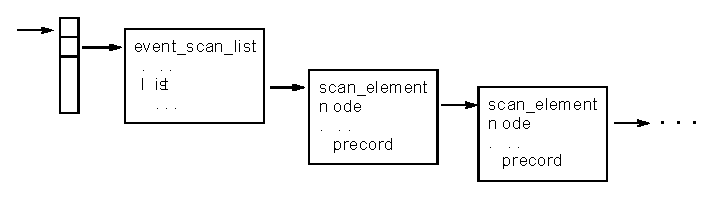
\includegraphics{scanning_12}
\end{center}

\subsubsection{post\_event} \index{post\_event}

\begin{verbatim}
post_event(int event)
\end{verbatim}

\index{post\_event}This routine is called to request event scanning.
It can be called from interrupt level.
It looks at each \verb|event_scan_list| referenced by \verb|pevent_list[*][event]| (one for each callback priority) and if any elements are present in the \verb|scan_list| a \verb|callbackRequest| is issued.
The appropriate callback task calls routine \verb|eventCallback|, which just calls \verb|scanList|. 

\subsection{I/O Event Scanning}

\index{I/O Event Scanning}
I/O event scanning is built around the following definitions:

\begin{verbatim}
typedef struct io_scan_list {
    CALLBACK            callback;
    scan_list           scan_list;
    struct io_scan_list *next;
}
static io_scan_list *iosl_head[NUM_CALLBACK_PRIORITIES] = {
    NULL,NULL,NULL};
\end{verbatim}

The array \verb|iosl_head| and the field \verb|next| are only kept so that \verb|scanpiol| can be implemented and will not be discussed further.
I/O event scanning uses the general purpose callback tasks to perform record processing, i.e. no task is spawned for I/O event.
The callback field of \verb|io_scan_list| is used to communicate with the callback tasks.

The following routines implement I/O event scanning:

\subsubsection{scanIoInit}

\begin{verbatim}
scanIoInit (IOSCANPVT  *ppioscanpvt)
\end{verbatim}

\index{scanIoInit}This routine is called by device or driver support.
It is called once for each interrupt source.
\verb|scanIoInit| allocates and initializes an array of \verb|io_scan_list| structures; one for each callback priority and puts the address in \verb|pioscanpvt|.
Three callback priorities are supported; low, medium, and high.
Thus for each interrupt source the structures are as illustrated below:

\begin{center}
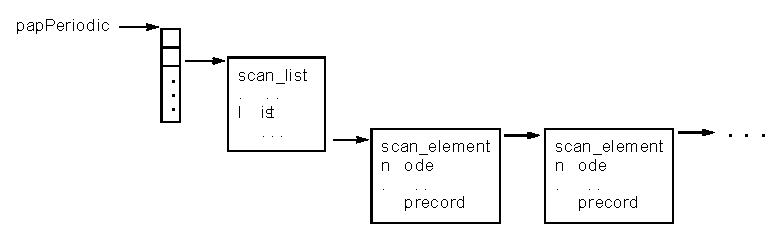
\includegraphics{scanning_19}
\end{center}

When \verb|scanAdd| or \verb|scanDelete| are called, they call the device support routine \verb|get_ioint_info| which returns \verb|pioscanpvt|.
The \verb|scan_element| is added or deleted from the correct scan list.

\subsubsection{scanIoRequest}

\begin{verbatim}
scanIoRequest (IOSCANPVT pioscanpvt)
\end{verbatim}

\index{scanIoRequest}This routine is called to request I/O event scanning.
It can be called from interrupt level.
It looks at each \verb|io_scan_list| referenced by \verb|pioscanpvt| (one for each callback priority) and if any elements are present in the \verb|scan_list| a \verb|callbackRequest| is issued.
The appropriate callback task calls routine \verb|ioeventCallback|, which just calls \verb|scanList|. 

\subsection{Periodic Scanning}

\index{Periodic Scanning}
Periodic scanning is built around the following definitions:

\begin{verbatim}
typedef struct periodic_scan_list {
    scan_list           scan_list;
    double              period;
    volatile enum ctl   scanCtl;
    epicsEventId        loopEvent;
} periodic_scan_list;
static int nPeriodic;
static periodic_scan_list **papPeriodic;
static epicsThreadId *periodicTaskId;
\end{verbatim}

\verb|nPeriodic|, which is determined at \verb|iocInit| time, is the number of periodic rates.
\verb|papPeriodic| is a pointer to an array of pointers to \verb|scan_lists|.
There is an array element for each scan rate.
Thus the structure illustrated in the figure below exists after \verb|iocInit|.

\begin{center}
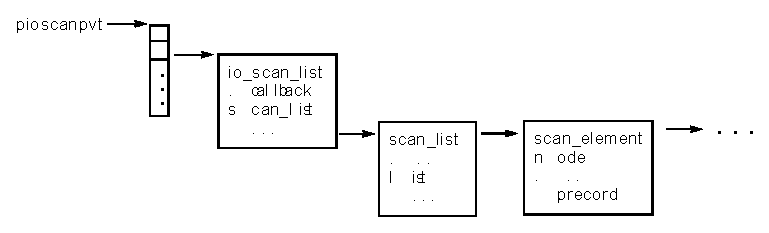
\includegraphics{scanning_1}
\end{center}

A periodic scan task is created for each scan rate.
The following routines implement periodic scanning:

\subsubsection{initPeriodic}

\begin{verbatim}
initPeriodic()
\end{verbatim}

\index{initPeriodic}This routine first determines the scan rates.
It does this by accessing the \verb|SCAN| field of the first record it finds.
It issues a call to \verb|dbGetField| with a \verb|DBR_ENUM| request.
This returns the menu choices for \verb|SCAN|.
From this the periodic rates are determined.
The array of pointers referenced by \verb|papPeriodic| is allocated.
For each scan rate a \verb|scan_list| is allocated and a \verb|periodicTask| is spawned.

\subsubsection{periodicTask}

\begin{verbatim}
periodicTask (struct scan_list *psl)
\end{verbatim}

\index{periodicTask}This task just performs an infinite loop, calling \verb|scanList| and then waiting until the start of the next scan interval, allowing for the time it took to scan the list.
If a periodic scan list takes longer to process than its defined scan period, the next scan will be delayed by half a scan period, with a maximum of 1 second delay.
This does not limit what scan rates can actually be implemented, as long as all the records in the list can be processed within the requested period.
Persistent over-runs (more than 10 times in a row) will result in a warning message being logged.
The total number of over-runs is counted by each scan thread and can be displayed using the \verb|scanppl| command.

\subsection{Scan Once}

\subsubsection{scanOnce}

\begin{verbatim}
void scanOnce (dbCommon *precord)
\end{verbatim}

\index{scanOnce}A task \verb|onceTask| waits for requests to issue a \verb|dbProcess| request.
The routine \verb|scanOnce| puts the address of the record to be processed in a ring buffer and wakes up \verb|onceTask|.

This routine can be called from interrupt level.

\subsubsection{SetQueueSize}

\verb|scanOnce| places its request on a ring buffer.
This is set by default to 1000 entries.
It can be changed by executing the following command in the startup script before \verb|iocInit|:

\begin{verbatim}
int scanOnceSetQueueSize(int size);
\end{verbatim}

\index{scanOnceSetQueueSize}








\chapter{\index{IOC Shell}\index{IOC Shell}IOC Shell}

\section{Introduction}

The EPICS IOC shell is a simple command interpreter which provides a subset of the capabilities of the vxWorks shell. It 
is used to interpret startup scripts (st.cmd) and to execute commands entered at the console terminal.  In most cases 
vxWorks startup scripts can be interpreted by the IOC shell without modification. The following sections of this chapter 
describe the operation of the IOC shell from the user's and programmer's points of view.

\section{IOC Shell Operation}

The IOC shell reads lines of input, expands environment variable parameters, breaks the line into commands and 
arguments then calls functions corresponding to the decoded command. Commands and arguments are separated by one 
or more `space' characters. Characters interpreted as spaces include the actual space character and the tab character as 
well as commas and open and close parentheses. Thus, the command line

\begin{verbatim}dbLoadRecords("db/dbExample1.db","user=mrk")
\end{verbatim}would be interpreted by the IOC shell as the \verb|dbLoadRecords| command with arguments d\verb|b/dbExample1.db| and 
\verb|user=mrk|.

Unrecognized commands result in a diagnostic message but are otherwise ignored.  Missing arguments are given a default 
value (0 for numeric arguments, NULL for string arguments).  Extra arguments are ignored.

Unlike the vxWorks shell, string arguments do not have to be enclosed in quotes unless they contain one or more of the 
space characters, in which case one of the quoting mechanisms described in the following section must be used.

\subsection{Environment variable parameter expansion}

Lines of input not beginning with a comment character (\verb|#|) are searched for character sequences of the form \$\{name\} or 
\$(name).  Such sequences are replaced with the value of the environment variable name before any other processing takes 
place.  Expansion is recursive so, for example,

\begin{verbatim}epics> epicsEnvSet v1 \${v2}
epics> epicsEnvSet v2 \${v3}
epics> epicsEnvSet v3 somePV
epics> dbpr ${v1}
\end{verbatim}will print information about the \verb|somePV| process variable - the \verb|${v1}| argument to the dbpr command expands to 
\verb|${v2}| which expands to \verb|${v3}| which expands to \verb|somePV|.  The backslashes in the definitions are needed to postpone 
the expansion, otherwise it would be done before the values of v1 and v2 are set.

\subsection{Quoting}

Quoting is used to remove the special meaning normally assigned to certain characters and can be used to include space or 
quote characters in arguments. Quoting can not be used to extend a command over more than one input line.

There are three quoting mechanisms: the backslash character, single quotes, and double quotes. A backslash (\textbackslash{}) preserves 
the literal value of the following character. Enclosing characters in single or double quotes preserves the literal value of 
each character (except a backslash) within the quotes, except that parameter expansion still occurs within double quotes.  
A single quote may occur between double quotes and a double quote may occur between single quotes.

\subsection{Command-line editing and history}

The IOC shell can use the readline or tecla library to obtain input from the console terminal. This provides full command-
line editing as well as easy access to previous commands through the command-line history capabilties provided by these 
libraries.  For full details, refer to the readline or tecla library documentation.  Command and argument completion is not 
supported.

If neither the readline nor tecla library is used the only command-line editing and history capabilities will be those 
supplied by the underlying operating system.  The console keyboard driver in Windows, for example, provides its own 
command-line editing and history commands.  On vxWorks the ledLib command-line input libraries are used.

\subsection{Redirection}

The IOC shell recognizes a subset of UNIX shell I/O redirection operators.  The redirection operators may precede, or 
appear anywhere within, or follow a command.  Redirections are processed in the order they appear, from left to right.   
Failure to open or create a file causes the redirection to fail and the command to be ignored.

Redirection of input causes the file whose name results from the  expansion  of  \verb|filename|  to  be  opened for reading on 
file descriptor \verb|n|, or the standard input (file descriptor 0) if \verb|n| is not specified.  The general format for redirecting input is:

\begin{verbatim}[n]<filename
\end{verbatim}As a special case, the IOC shell recognizes a standard input redirection appearing by itself (i.e. with no command) as a 
request to read commands from \verb|filename| until an exit command or EOF is encountered. The IOC shell then resumes 
reading commands from the current source. Commands read from \verb|filename| are not added to the readline command 
history. The level of nesting is limited only by the maximum number of files that can be open simultaneously.

Redirection of output causes the  file  whose  name  results from  the expansion of \verb|filename| to be opened for writing on 
file descriptor \verb|n|, or the standard output (file descriptor 1)  if \verb|n|  is  not  specified.   If  the  file  does not exist it is created; 
if it does exist it is truncated to zero size. The general format for redirecting output is:

\begin{verbatim}[n]>filename
\end{verbatim} The general format for appending output is:

\begin{verbatim}[n]>>filename
\end{verbatim}Redirection of output in this fashion causes the \verb|filename| to be opened for appending on file descriptor \verb|n|, or the 
standard output (file descriptor  1)  if \verb|n| is not specified.  If the file does not exist it is created.

\subsection{Utility Commands}

The IOC shell recognizes the following commands as well as the commands described in chapter 6 (Database Design) and 
chapter 9 (IOC Test Facilities) among others.  In addition, the commands described in the sequencer documentation are 
recognized.
\begin{center}\begin{longtable}{p{1.59082in}p{5.21418in}}
Command & Description\\
\hline
help [command ...] & Display synopsis of specified commands.  Wild-card matching is applied so `help db*' displays a synopsis of all commands beginning with the letters `db'.With no arguments display a list of all commands.\\
\# & A `\#' in the first column of a line indicates the beginning of a comment which continues to the end of the line\\
exit & Stop reading commands. When the top-level command interpreter encounters an exit command or end-of-file (EOF) it returns to its caller.\\
cd directory & Change working directory to directory.\\
pwd & Print the name of the working directory.\\
var [name [value]] & If both arguments are present, assign the value to the named variable.If only the name argument is present, print the current value of that variable.If neither argument is present, print the value of all variables registered with the shell.  Variables are registered in application database definitions using the variable keyword as described in Section6.9 on page104.\\
show [-level] [task ...] & Show information about specified tasks.  If no task arguments are present, show information on all tasks.  The level argument controls the amount of information printed.  The default level is 0.  The task arguments can be task names or task i.d. numbers.\\
system command\_string & Send command\_string to the system command interpreter for execution.  This command is present only if some application database definition file contains registrar(iocshSystemCommand) and if the system provides a suitable command interpreter (vxWorks does not).\\
epicsEnvSet name value & Set environment variable name to the specified value.\\
epicsEnvShow  [name] & If no name is specified the names and values of all environment variables will be shown. If a name is specified the value of that environment variable will be shown.\\
epicsParamShow & Show names and values of all EPICS configuration parameters.\\
iocLogInit & Initialize IOC logging.\\
epicsThreadSleep sec & Pause execution of IOC shell for sec seconds.
\end{longtable}\end{center}


The \verb|var| command is intended for simple applications such as setting the value of debugging flags.  Applications which 
require more complex expression handling should use the cexp package.

A \index{spy}\verb|spy| command to show periodic activity reports is available on RTEMS as part of the RTEMS\_UTILS support module.  
The following changes must be made to add this command to an application.

\begin{itemize}\item Add an RTEMS\_UTILS entry to the application configure/RELEASE file.

\item Add \verb|spy.dbd| to the list of application dbd files and \verb|rtemsutils| to the list of application libraries in the 
application Makefile.

\end{itemize}\subsection{ENVIRONMENT VARIABLES}

The IOC shell uses the following environment variables to control its operation.
\begin{center}\begin{longtable}{p{1.305in}p{5.46in}}
Variable & Description\\
\hline
IOCSH\_PS1 & Prompt string. Default is ``epics\textgreater{} ``.\\
IOCSH\_HISTSIZE & Number of previous command lines to remember. If the IOCSH\_HISTSIZE environment variable is not present the value of the HISTSIZE environment variable is used.  In the absence of both environment variables, 10 command lines will be remembered.\\
TERM, INPUTRC & These and other environment variables are used by the readline and termcap libraries and are described in the documentation for those libraries.
\end{longtable}\end{center}


\section{IOC Shell Programming}

The declarations described in this section are included in the \verb|iocsh.h| header file.

\index{iocsh.h}\subsection{Invoking the IOC shell}

The prototypes for calling the IOC shell command interpreter are:

\begin{verbatim}int iocsh(const char *pathname);
int iocshCmd(const char *cmd);
\end{verbatim}\index{iocsh}
\index{iocshCmd}The pathname argument to the \verb|iocsh| function is the name of the file from which commands are to be read.  If the 
pathname argument is NULL, commands are read from the standard input and prompts are issued to the standard output.  
Commands are read until an \verb|exit| command is encountered or until end-of-file is reached, at which point iocsh returns a 
value of 0.  If the specified file can not be opened iocsh returns -1.

The IOC shell can be invoked from  the vxWorks shell, either from within a vxWorks startup script or from vxWorks 
command-line interpreter, using

\begin{verbatim}iocsh "script"
\end{verbatim}to read from an IOC shell script.  It can also be invoked from the vxWorks command-line interpreter with no argument in 
which case the IOC shell takes over the duties of command-line interaction.

The \verb|iocshCmd| function takes a single IOC shell command and executes it. The function may be called from any thread, 
but many of the commands are not necessarily thread-safe so this should only be used with care. The function is most 
useful to execute a single IOC shell command from a vxWorks startup script or command line, like this:

\begin{verbatim}iocshCmd "iocsh command string"
\end{verbatim}The stdio stream redirection and environment variable expansion processes described above are performed on the string 
as part of the execution process.

\subsection{Registering Commands}

Commands must be registered before they can be recognized by the IOC shell.  Registration is achieved by calling  the 
registration function:

\begin{verbatim} void iocshRegister(const iocshFuncDef *piocshFuncDef, iocshCallFunc func);
\end{verbatim}\index{iocshRegister}The first argument is a pointer to a data structure which describes the command and any arguments it may take.  The 
second argument is a pointer to a function which will be called by iocsh when the corresponding command is 
encountered.

The command is described by the  \verb|iocshFuncDef |structure:

\begin{verbatim}struct iocshFuncDef {
    const char *name;
    int nargs;
    const iocshArg * const *arg;
};
\end{verbatim}\index{iocshFuncDef}The name element is the name of the command.  The arg element is a pointer to an array of pointers to structures each of 
which defines a single argument.  The nargs element declares the number of entries in the array of pointers to the 
argument descriptions.  If nargs is zero, arg can be NULL.  The structures which define each of the arguments is:

\begin{verbatim}struct iocshArg {
    const char *name;
    iocshArgType type;
}iocshArg;
\end{verbatim}\index{iocshArg}The name element is used by the help command to print a synopsis for the command.  The type element describes the type 
of the argument and takes one of the following values:
\begin{center}\begin{longtable}{p{1.5in}p{3.76in}}
Type Specifier & Description\\
\hline
iocshArgInt & The argument will be converted to an integer value.\\
iocshArgDouble & The argument will be converted to a double-precision floating point value.\\
iocshArgString & The argument will be left as a string.  The memory used to hold the string is `owned' by iocsh and will be reused once the handler function returns.\\
iocshArgPersistentString & A copy of the argument will be made and a pointer to the copy will be passed to the handler.  The called function can release this copy by using the pointer as an argument to free().\\
iocshArgPdbbase & The argument must be pdbbase.\\
iocshArgArgv & An arbitrary number of arguments is expected.  Subsequent iocshArg structures will be ignored.
\end{longtable}\end{center}


The `handler' function which is called when its corresponding command is recognized should be of the form:

\begin{verbatim}    void showCallFunc(const iocshArgBuf *args);
\end{verbatim}The argument to the handler function is a pointer to an array of unions.  The number of elements in this array is equal to 
the number of arguments specified in the structure describing the command.  The type and name of the union element 
which contains the argument value depends on the `type' element of the corresponding argument descriptor:
\begin{center}\begin{longtable}{p{1.45833in}p{0.56in}p{1.19in}}
Type Specifier & Type & Union element\\
\hline
iocshArgInt & int & args[i].ival\\
iocshArgDouble & double & args[i].dval\\
iocshArgStringiocshArgPersistentString & char * & args[i].sval\\
iocshArgPdbbase & void * & args[i].vval\\
iocshArgArgv & intchar ** & args[i].aval.acargs[i].aval.av
\end{longtable}\end{center}


If an \verb|iocshArgArgv |argument type is present it is often the first and only argument specified for the command.  In this 
case, \verb|args[0].aval.av[0]| will be the name of the command,  \verb|args[0].aval.av[1]| will be the first argument, 
and so on.

\subsection{Registrar Command Registration}

\index{registrar:iocsh commands}Commands are normally registered with the IOC shell in a registrar function. The application's database description file 
uses the \verb|registrar| keyword to specify a function which will be called from the EPICS initialization code during the 
application startup process.  This function then calls \verb|iocshRegister| to register its commands with the iocsh.

\index{registrar}The following code fragments shows how this can be performed for an example driver.

\begin{verbatim}#include <iocsh.h>
#include <epicsExport.h>

/* drvXxx code, FuncDef and CallFunc definitions ... */

static void drvXxxRegistrar(void)
{
    iocshRegister(&drvXxxConfigureFuncDef, drvXxxConfigureCallFunc);
}
epicsExportRegistrar(drvXxxRegistrar);
\end{verbatim}To include this driver in an application a developer would then add

\begin{verbatim}registrar(drvXxxRegistrar)
\end{verbatim}to an application database description file.

\subsection{Automatic Command Registration}

A C++ static constructor can also be used to register IOC shell commands before the EPICS application begins. The 
following example shows how the \verb|epicsThreadSleep| command could be described and registered.

\begin{verbatim}#include <iocsh.h>

static const iocshArg epicsThreadSleepArg0 = { "seconds",iocshArgDouble};
static const iocshArg *const epicsThreadSleepArgs[1] =
    {&epicsThreadSleepArg0};
static const iocshFuncDef epicsThreadSleepFuncDef =
    {"epicsThreadSleep",1,epicsThreadSleepArgs};
static void epicsThreadSleepCallFunc(const iocshArgBuf *args)
{
    epicsThreadSleep(args[0].dval);
}

static int doRegister(void)
{
    iocshRegister(epicsThreadSleepFuncDef, epicsThreadSleepCallFunc);
    return 1;
}
static int done = doRegister();
\end{verbatim}



\chapter{libCom}

This chapter and the next describe the facilities provided in \verb|<base>/src/libCom|.
This chapter describes facilities which are platform independent.
The next chapter describes facilities which have different implementations on different platforms.

\section{bucketLib}

\index{bucketLib.h}
\verb|bucketLib.h| describes a hash facility for integers, pointers, and strings.
It is used by the Channel Access Server.
It is currently undocumented.

\section{calc}

\index{postfix.h}
\verb|postfix.h| defines several macros and the routines used by the calculation record type calcRecord, access security, and other code, to compile and evaluate mathematical expressions.
The syntax of the infix expressions accepted is described below.

\begin{verbatim}
long postfix(const char *psrc, char *ppostfix, short *perror);
long calcArgUsage(const char *ppostfix, unsigned long *pinputs,
    unsigned long *pstores);
const char * calcErrorStr(short error);
long calcPerform(double *parg, double *presult, const char *ppostfix);
\end{verbatim}

\index{postfix}
\index{calcArgUsage}
\index{calcErrorStr}
\index{calcPerform}
The postfix() routine converts an expression from infix to postfix notation.
It is the callers's responsibility to make sure that \emph{ppostfix} points to sufficient storage to hold the postfix expression;
the macro \index{INFIX\_TO\_POSTFIX\_SIZE}\verb|INFIX_TO_POSTFIX_SIZE(n)| can be used to calculate an appropriate buffer from the length of the infix string.
There is no longer a maximum length to the input expression that can be accepted, although there are internal limits to the complexity of the expressions that can be converted and evaluated.
If postfix() returns a non-zero value it will have placed an error code at the location pointed to by \emph{perror}.
\index{CALC\_ERR\_}
The error codes used are defined in \verb|postfix.h| as a series of macros with names starting \verb|CALC_ERR_|, but a string representation of the error code is more useful and can be obtained by passing the value to the calcErrorStr() routine, which returns a static error message string explaining the error.

Software using the calc subsystem may need to know what expression arguments are used and/or modified by a particular expression.
It can discover this from the postfix string by calling calcArgUsage(), which takes two pointers \emph{pinputs} and \emph{pstores} to a pair of unsigned long bitmaps which return that information to the caller.
Passing a NULL value for either of these pointers is legal if only the other is needed.
The least signficant bit (bit 0) of the bitmap at *\emph{pinputs} will be set if the expression depends on the argument A, and so on through bit 11 for the argument L.
Similarly, bit 0 of the bitmap at *\emph{pstores} will be set if the expression assigns a value to the argument A.
An argument that is not used until after a value has been assigned to it will not be set in the \emph{pinputs} bitmap, thus the bits can be used to determine whether a value needs to be supplied for their associated argument or not for the purposes of evaluating the expression.
The return value from calcArgUsage() will be non-zero if the \emph{ppostfix} expression was illegal, otherwise 0.

The postfix expression is evaluated by calling the calcPerform() routine, which returns the status values 0 for OK, or non-zero if an error is discovered during the evaluation process.

The arguments to calcPerform() are:

\begin{description}
\item \emph{parg} - Pointer to an array of double values for the arguments A-L that can appear in the expression.
Note that the argument values may be modified if the expression uses the assignment operator.

\item \emph{presult} - Where to put the calculated result, which may be a NaN or Infinity.

\item \emph{ppostfix} - The postfix expression created by postfix().

\end{description}

\subsection{Infix Expression Syntax}

\index{Expression Syntax}
The infix expressions that can be used are very similar to the C expression syntax, but with some additions and subtle differences in operator meaning and precedence.
The string may contain a series of expressions separated by a semi-colon character `\verb|;|' any one of which may actually provide the calculation result;
however all of the other expressions included must assign their result to a variable.
All alphabetic elements described below are case independent, so upper and lower case letters may be used and mixed in the variable and function names as desired.
Spaces may be used anywhere within an expression except between the characters that make up a single expression element.

\subsubsection{Numeric Literals}

The simplest expression element is a numeric literal, any (positive) number expressed using the standard floating point syntax that can be stored as a double precision value.
This now includes the values \verb|Infinity| and \verb|NaN| (not a number).
Note that negative numbers will be encoded as a positive literal to which the unary negate operator is applied.

Examples:

\begin{verbatim}
1
2.718281828459
Inf
\end{verbatim}

\subsubsection{Constants}

There are three trigonometric constants available to any expression which return a value:

\begin{itemize}
\item \verb|pi| returns the value of the mathematical constant $\pi$.

\item \verb|D2R| evaluates to $\pi$/180 which, when used as a multiplier, converts an angle from degrees to radians.

\item \verb|R2D| evaluates to 180/$\pi$ which as a multiplier converts an angle from radians to degrees.

\end{itemize}

\subsubsection{Variables}

Variables are used to provide inputs to an expression, and are named using the single letters \verb|A| through \verb|L| inclusive or the keyword \verb|VAL| which refers to the previous result of this calculation.
The software that makes use of the expression evaluation code should document how the individual variables are given values;
for the calc record type the input links INPA through INPL can be used to obtain these from other record fields, and \verb|VAL| refers to the the VAL field (which can be overwritten from outside the record via Channel Access or a database link).

\subsubsection{Variable Assignment Operator}

Recently added is the ability to assign the result of a sub-expression to any of the single letter variables, which can then be used in another sub-expression.
The variable assignment operator is the character pair \verb|:=| and must immediately follow 
the name of the variable to receive the expression value.
Since the infix string must return exactly one value, every expression string must have exactly one sub-expression that is not an assignment, which can appear anywhere in the string.
Sub-expressions within the string are separated by a semi-colon character.

Examples:

\begin{verbatim}
B; B:=A
i:=i+1; a*sin(i*D2R)
\end{verbatim}

\subsubsection{Arithmetic Operators}

The usual binary arithmetic operators are provided:
\verb|+ - *| and \verb|/| with their usual relative precedence and left-to-right associativity, and \verb|-| may also be used as a unary negate operator where it has a higher precedence and associates from right to left.
There is no unary plus operator, so numeric literals cannot begin with a + sign.

Examples:

\begin{verbatim}
a*b + c
a/-4 - b
\end{verbatim}

Three other binary operators are also provided:
\verb|%| is the integer modulo operator, while the synonymous operators \verb|**| and \verb|^| raise their left operand to the power of the right operand.
\verb|%| has the same precedence and associativity as \verb|*| and \verb|/|, while the power operators associate left-to-right and have a precedence in between \verb|*| and unary minus.

Examples:

\begin{verbatim}
e:=a%10; d:=a/10%10; c:=a/100%10; b:=a/1000%10; b*4096+c*256+d*16+e
sqrt(a**2 + b**2)
\end{verbatim}

\subsubsection{Algebraic Functions}

Various algebraic functions are available which take parameters inside parentheses.
The parameter seperator is a comma.

\begin{itemize}
\item Absolute value: \verb|abs(a)|

\item Exponential e\textsuperscript{a}: \verb|exp(a)|

\item Logarithm, base 10: \verb|log(a)|

\item Natural logarithm (base e): \verb|ln(a)| \emph{or} \verb|loge(a)|

\item \emph{n} parameter maximum value: \verb|max(a, b, ...)|

\item \emph{n} parameter minimum value: \verb|min(a, b, ...)|

\item Square root: \verb|sqr(a)| \emph{or} \verb|sqrt(a)|

\end{itemize}

\subsubsection{Trigonometric Functions}

Standard circular trigonometric functions, with angles expressed in radians:

\begin{itemize}
\item Sine: \verb|sin(a)|

\item Cosine: \verb|cos(a)|

\item Tangent: \verb|tan(a)|

\item Arcsine: \verb|asin(a)|

\item Arccosine: \verb|acos(a)|

\item Arctangent: \verb|atan(a)|

\item 2 parameter arctangent:
\verb|atan2(a, b)| \emph{- Note that these arguments are the reverse of the ANSI C function, so while C would return arctan(a/b) the calc expression engine returns arctan(b/a)}

\end{itemize}

\subsubsection{Hyperbolic Trigonometry}

The basic hyperbolic functions are provided, but no inverse functions (which are not provided by the ANSI C math library either).

\begin{itemize}
\item Hyperbolic sine: \verb|sinh(a)|

\item Hyperbolic cosine: \verb|cosh(a)|

\item Hyperbolic tangent: \verb|tanh(a)|

\end{itemize}

\subsubsection{Numeric Functions}

The numeric functions perform operations related to the floating point numeric representation and truncation or rounding.

\begin{itemize}
\item Round up to next integer: \verb|ceil(a)|

\item Round down to next integer: \verb|floor(a)|

\item Round to nearest integer: \verb|nint(a)|

\item Test for infinite result: \verb|isinf(a)|

\item Test for any non-numeric values: \verb|isnan(a, ...)|

\item Test for all finite, numeric values: \verb|finite(a, ...)|

\item Random number between 0 and 1: \verb|rndm|

\end{itemize}

\subsubsection{Boolean Operators}

These operators regard their arguments as true or false, where 0.0 is false and any other value is true.

\begin{itemize}
\item Boolean and: \verb|a && b|

\item Boolean or: \verb+a || b+

\item Boolean not: \verb|!a|

\end{itemize}

\subsubsection{Bitwise Operators}

The bitwise operators convert their arguments to an integer (by truncation), perform the appropriate bitwise operation and convert back to a floating point value.
Unlike in C though, \verb|^| is \emph{not} a bitwise exclusive-or operator.

\begin{itemize}
\item Bitwise and: \verb|a & b| \emph{or} \verb|a and b|

\item Bitwise or: \verb+a | b+ \emph{or} \verb|a or b|

\item Bitwise exclusive or: \verb|a xor b|

\item Bitwise not (ones complement): \verb|~a| \emph{or} \verb|not a|

\item Bitwise left shift: \verb|a << b|

\item Bitwise right shift: \verb|a >> b|

\end{itemize}

\subsubsection{Relational Operators}

Standard numeric comparisons between two values:

\begin{itemize}
\item Less than: \verb|a < b|

\item Less than or equal to: \verb|a <= b|

\item Equal to: \verb|a = b| \emph{or} \verb|a == b|

\item Greater than or equal to: \verb|a >= b|

\item Greater than: \verb|a > b|

\item Not equal to: \verb|a != b| \emph{or} \verb|a # b|

\end{itemize}

\subsubsection{Conditional Operator}

Expressions can use the C conditional operator, which has a lower precedence than all of the other operators except for the assignment operator.

\begin{itemize}
\item \emph{condition} \verb|?| \emph{true result} \verb|:| \emph{false result}

\end{itemize}

Example:

\begin{verbatim}
a < 360 ? a+1 : 0
\end{verbatim}

\subsubsection{Parentheses}

Sub-expressions can be placed within parentheses to override operator precence rules.
Parentheses can be nested to any depth, but the intermediate value stack used by the expression evaluation engine is limited to 80 results (which requirea an expression at least 321 characters long to reach).

\section{cppStd}

\index{class templates}
\index{function templates}
\index{templates}
\index{standard C++ library}
\index{ISO C++}
\index{C++ library}
This subdirectory of libCom is intended for facilities such as class and function templates that implement parts of the ISO standard C++ library where such facilities are not available or not efficient on all the target platforms on which EPICS is supported.
EPICS does not make use of the C++ container templates because the large number of memory allocation and deletion operations that these use causes memory pool fragmentation on some platforms, threatening the lifetime of an individual IOC.

\subsection{epicsAlgorithm}

\index{epicsAlgorithm.h}
\index{algorithm}
\index{std::min}
\index{std::max}
\index{std::swap}
\index{epicsMin}
\index{epicsMax}
\index{epicsSwap}
\verb|epicsAlgorithm.h| contains a few templates that are also available in the C++ standard header \verb|algorithm|, but are provided here in a much smaller file.
\verb|algorithm| contains many templates for sorting and searching through C++ template containers which are not used in EPICS.
If all you need from there is \verb|std::min()|, \verb|std::max()| and/or \verb|std::swap()| your code may compile faster if you include \verb|epicsAlgorithm.h| and use \verb|epicsMin()|, \verb|epicsMax()| and \verb|epicsSwap()| instead.

\begin{center}
\begin{longtable}{p{1.5in}p{4.25in}}
\textbf{Template Function} & \textbf{Meaning}\\
\hline
epicsMin(a, b) & Returns the smaller of a or b compared using a\textless{}b. Handles NaNs correctly.\\
epicsMax(a, b) & Returns the larger of a or b compared using a\textless{}b. Handles NaNa correctly.\\
epicsSwap(a, b) & Swaps the values of a and b; the data type must support both copy-construction and assignment.
\end{longtable}

\end{center}


\section{epicsExit}

\index{epicsExit}
\begin{verbatim}
void epicsExit(int status);
void epicsExitCallAtExits(void);
void epicsAtExit(void (*epicsExitFunc)(void *arg), void *arg);
void epicsExitCallAtThreadExits(void);
int  epicsAtThreadExit(void (*epicsExitFunc)(void *arg), void *arg);
\end{verbatim}

\index{epicsExit}
\index{epicsExitCallAtExits}
\index{epicsAtExit}
\index{epicsExitCallAtThreadExits}
\index{epicsAtThreadExit}
This is an extended replacement for the Posix \verb|exit| and \verb|atexit| routines, which also provides a pointer argument to pass to the exit handlers.
This facility was created because of problems on vxWorks and windows with the implementation of \verb|atexit|, i.e. neither of these systems implement \verb|exit| and \verb|atexit| according to the POSIX standard.

\begin{center}
\begin{longtable}{p{2.0in}p{4.4in}}
\textbf{Method} & \textbf{Meaning}\\
\hline
epicsExit & This calls epicsExitCallAtExits and then passes status on to exit.\\
epicsExitCallAtExits & This calls each of the functions registered by prior calls to epicsAtExit, in reverse order of their registration.  Most applications will not call this routine directly.\\
epicsAtExit & Register a function and an associated context parameter, to be called with the given parameter when epicsExitCallAtExits is invoked.\\
epicsExitCallAtThreadExits & This calls each of the functions that were registered by the current thread calling epicsAtThreadExit, in reverse order of the function registration.  This routine is called automatically when an epicsThread's main entry method returns, but will not be run if the thread is stopped by other means.\\
epicsAtThreadExit & Register a function and an associated context parameter. The function will be called with the given parameter when epicsExitCallAtThreadExits is invoked by the current thread ending normally, i.e. when the thread function returns.
\end{longtable}

\end{center}


\section{cvtFast}

\verb|cvtFast.h| provides routines for converting various numeric types into an ascii string.
They offer a combination of speed and convenience not available with sprintf().

\index{cvtFast.h}
\index{cvtFloatToString}
\index{cvtDoubleToString}
\index{cvtFloatToExpString}
\index{cvtDoubleToExpString}
\index{cvtFloatToCompactString}
\index{cvtDoubleToCompactString}
\index{cvtCharToString}
\index{cvtUcharToString}
\index{cvtShortToString}
\index{cvtUshortToString}
\index{cvtLongToString}
\index{cvtUlongToString}
\index{cvtLongToHexString}
\index{cvtLongToOctalString}
\index{cvtBitsToUlong}
\index{cvtUlongToBits}
\begin{verbatim}
/* These functions return the number of ASCII characters generated */
int cvtFloatToString(float value, char *pstr, unsigned short precision);
int cvtDoubleToString(double value, char *pstr, unsigned short prec);
int cvtFloatToExpString(float value, char *pstr, unsigned short prec);
int cvtDoubleToExpString(double value, char *pstr, unsigned short prec);
int cvtFloatToCompactString(float value, char *pstr, unsigned short prec);
int cvtDoubleToCompactString(double value, char *pstr, unsigned short prec);
int cvtCharToString(char value, char *pstring);
int cvtUcharToString(unsigned char value, char *pstr);
int cvtShortToString(short value, char *pstr);
int cvtUshortToString(unsigned short value, char *pstr);
int cvtLongToString(epicsInt32 value, char *pstr);
int cvtUlongToString(epicsUInt32 value, char *pstr);
int cvtLongToHexString(epicsInt32 value, char *pstr);
int cvtLongToOctalString(epicsInt32 value, char *pstr);
unsigned long cvtBitsToUlong(
        epicsUInt32 src,
        unsigned bitFieldOffset,
        unsigned bitFieldLength);
unsigned long cvtUlongToBits(
        epicsUInt32 src,
        epicsUInt32 dest,
        unsigned bitFieldOffset,
        unsigned bitFieldLength);
\end{verbatim}

\section{cxxTemplates}

This directory contains various C++ template headers and APIs:

\begin{itemize}

\item \verb|epicsGuard.h| - Mutex guard classes

\item \verb|epicsSingleton.h| - Single object enforcement

\item \verb|resourceLib.h| - Hash tables

\item \verb|tsDLList.h| - Double Linked Lists

\item \verb|tsFreeList.h| - Free List for efficient new/delete

\item \verb|tsSLList.h| - Single Linked Lists

\end{itemize}

\index{resourceLib.h}
\index{tsDLList.h}
\index{tsFreeList.h}
\index{tsSLList.h}
Currently these are only being used by Channel Access Clients and the portable Channel Access Server.

\section{dbmf}

\verb|dbmf.h| (Database Macro/Free) describes a facility that prevents memory fragmentation when memory is allocated and then freed a short time later.

\index{dbmf.h}
Routines within iocCore like dbLoadDatabase() have the following attributes:

\begin{itemize}
\item They repeatedly call malloc() followed soon afterwards by a call to free() the temporarily allocated storage.

\item Between those calls to malloc() and free(), an additional call to malloc() is made that does NOT have an associated free().

\end{itemize}

In some environments, e.g. vxWorks 5.x, this behavior causes severe memory fragmentation.

The dbmf facility stops the memory fragmentation.
It should NOT be used by code that allocates storage and then keeps it for a considerable period of time before releasing.
Such code can use the freeList library described below.

\begin{verbatim}
int dbmfInit(size_t size, int chunkItems);
void *dbmfMalloc(size_t bytes);
void dbmfFree(void* bytes);
void dbmfFreeChunks(void);
int dbmfShow(int level);
\end{verbatim}

\index{dbmfInit}
\index{dbmfMalloc}
\index{dbmfFree}
\index{dbmfFreeChunks}
\index{dbmfShow}
\begin{center}
\begin{longtable}{p{1.3in}p{4.5in}}
\textbf{Routine} & \textbf{Meaning}\\
\hline
dbmfInit() & Initialize the facility. Each time malloc() must be called size*chunkItems bytes are allocated. size is the maximum size request from dbmfMalloc() that will be allocated from the dbmf pool. If dbmfInit() was not called before one of the other routines then it is automatically called with size=64 and chuckItems=10.\\
dbmfMalloc() & Allocate memory. If bytes is \textgreater{} size then malloc() is used to allocate the memory.\\
dbmfFree() & Free the memory allocated by dbmfMalloc().\\
dbmfFreeChunks() & Free all chunks that have contain only free items.\\
dbmfShow() & Show the status of the dbmf memory pool.
\end{longtable}

\end{center}


\section{ellLib}

\verb|ellLib.h| describes a double linked list library. It provides functionality similar to the vxWorks lstLib library. See the 
vxWorks documentation for details. There is an ellXXX() routine to replace most vxWorks lstXXX() routines.

\index{ellLib.h}
\begin{verbatim}
typedef struct ELLNODE {
  struct ELLNODE  *next;
  struct ELLNODE  *previous;
}ELLNODE;

typedef void (*FREEFUNC)(void *);

typedef struct ELLLIST {
  ELLNODE  node;
  int   count;
void ellInit (ELLLIST *pList);
int ellCount (ELLLIST *pList);
ELLNODE *ellFirst (ELLLIST *pList);
ELLNODE *ellLast (ELLLIST *pList);
ELLNODE *ellNext (ELLNODE *pNode);
ELLNODE *ellPrevious (ELLNODE *pNode);
void ellAdd (ELLLIST *pList, ELLNODE *pNode);
void ellConcat (ELLLIST *pDstList, ELLLIST *pAddList);
void ellDelete (ELLLIST *pList, ELLNODE *pNode);
void ellExtract (ELLLIST *pSrcList, ELLNODE *pStartNode,
    ELLNODE *pEndNode, ELLLIST *pDstList);
ELLNODE *ellGet (ELLLIST *pList);
void ellInsert (ELLLIST *plist, ELLNODE *pPrev, ELLNODE *pNode);
ELLNODE *ellNth (ELLLIST *pList, int nodeNum);
ELLNODE *ellNStep (ELLNODE *pNode, int nStep);
int ellFind (ELLLIST *pList, ELLNODE *pNode);
void ellFree2 (ELLLIST *pList, FREEFUNC freeFunc);
void ellFree (ELLLIST *pList);    // Use only if freeFunc is free()
void ellVerify (ELLLIST *pList);
\end{verbatim}

\index{ELLNODE}
\index{ELLLIST}
\index{ellInit}
\index{ellCount}
\index{ellFirst}
\index{ellLast}
\index{ellNext}
\index{ellPrevious}
\index{ellAdd}
\index{ellConcat}
\index{ellDelete}
\index{ellExtract}
\index{ellGet}
\index{ellInsert}
\index{ellNth}
\index{ellNStep}
\index{ellFind}
\index{ellFree2}
\index{ellFree}
\index{ellVerify}


\section{epicsRingBytes}

\index{epicsRingBytes}
\index{epicsRingBytes.h}
\verb|epicsRingBytes.h| describes a C facility for a commonly used type of ring buffer.

\subsection{C interface}

EpicsRingBytes provides methods for creating and using ring buffers (first in first out circular buffers) that store bytes.
The unlocked variant is designed so that one writer thread and one reader thread can access the ring simultaneously without requiring mutual exclusion.
The locked variant uses an epicsSpinLock, and works with any numbers of writer and reader threads.

\index{epicsRingBytes.h}
\begin{verbatim}
epicsRingBytesId epicsRingBytesCreate(int nbytes);
epicsRingBytesId epicsRingBytesLockedCreate(int nbytes);
void epicsRingBytesDelete(epicsRingBytesId id);
int epicsRingBytesGet(epicsRingBytesId id, char *value,int nbytes);
int epicsRingBytesPut(epicsRingBytesId id, char *value,int nbytes);
void epicsRingBytesFlush(epicsRingBytesId id);
int epicsRingBytesFreeBytes(epicsRingBytesId id);
int epicsRingBytesUsedBytes(epicsRingBytesId id);
int epicsRingBytesSize(epicsRingBytesId id);
int epicsRingBytesIsEmpty(epicsRingBytesId id);
int epicsRingBytesIsFull(epicsRingBytesId id);
\end{verbatim}

\index{epicsRingBytesId}
\index{epicsRingBytesCreate}
\index{epicsRingBytesLockedCreate}
\index{epicsRingBytesDelete}
\index{epicsRingBytesGet}
\index{epicsRingBytesPut}
\index{epicsRingBytesFlush}
\index{epicsRingBytesFreeBytes}
\index{epicsRingBytesUsedBytes}
\index{epicsRingBytesSize}
\index{epicsRingBytesIsEmpty}
\index{epicsRingBytesIsFull}
\begin{center}
\begin{longtable}{p{1.75in}p{4.25in}}
\textbf{Method} & \textbf{Meaning}\\
\hline
epicsRingBytesCreate() & Create a new ring buffer of size nbytes. The returned epicsRingBytesId is passed to the other ring methods.\\
epicsRingBytesLockedCreate() & Same as epicsRingBytesCreate, but create the spin lock secured variant of the ring buffer.\\
epicsRingBytesDelete() & Delete the ring buffer and free any associated memory.\\
epicsRingBytesGet() & Move up to nbytes from the ring buffer to value. The number of bytes actually moved is returned.\\
epicsRingBytesPut() & Move nbytes from value to the ring buffer if there is enough free space available to hold them. The number of bytes actually moved is returned, which will be zero if insufficient space exists.\\
epicsRingBytesFlush() & Make the ring buffer empty.\\
epicsRingBytesFreeBytes() & Return the number of free bytes in the ring buffer.\\
epicsRingBytesUsedBytes() & Return the number of bytes currently stored in the ring buffer.\\
epicsRingBytesSize() & Return the size of the ring buffer, i.e., nbytes specified in the call to epicsRingBytesCreate().\\
epicsRingBytesIsEmpty() & Return (true, false) if the ring buffer is currently empty.\\
epicsRingBytesIsFull() & Return (true, false) if the ring buffer is currently empty.
\end{longtable}

\end{center}


epicsRingBytes has the following properties:

\begin{itemize}
\item For a ring buffer with a single writer it is not necessary to lock epicsRingBytesPut() calls.

\item For a ring buffer with a single reader it is not necessary to lock epicsRingBytesGet() calls.

\item epicsRingBytesFlush() should only be used when both gets and puts are locked out.

\end{itemize}


\section{epicsRingPointer}

\index{epicsRingPointer}
\index{epicsRingPointer.h}
\verb|epicsRingPointer.h| describes a C++ and a C facility for a commonly used type of ring buffer.

\subsection{C++ Interface}

EpicsRingPointer provides methods for creating and using ring buffers (first in first out circular buffers) that store pointers.
The unlocked variant is designed so that one writer thread and one reader thread can access the ring simultaneously without requiring mutual exclusion.
The locked variant uses an epicsSpinLock, and works with any numbers of writer and reader threads.

\begin{verbatim}
template <class T>
class epicsRingPointer {
public:
    epicsRingPointer(int size, bool locked);
    ~epicsRingPointer();
    bool push(T *p);
    T* pop();
    void flush();
    int getFree() const;
    int getUsed() const;
    int getSize() const;
    bool isEmpty() const;
    bool isFull() const;

private: // Prevent compiler-generated member functions
    // default constructor, copy constructor, assignment operator
    epicsRingPointer();
    epicsRingPointer(const epicsRingPointer &);
    epicsRingPointer& operator=(const epicsRingPointer &);

private: // Data
    ...
};
\end{verbatim}

\index{ringPointer}
An epicsRingPointer cannot be assigned to, copy-constructed, or constructed without giving the \emph{size} argument.
The C++ compiler will object to some of the statements below:

\begin{verbatim}
epicsRingPointer rp0();   // Error: default constructor is private
epicsRingPointer rp1(10); // OK
epicsRingPointer rp2(t1); // Error: copy constructor is private
epicsRingPointer *prp;    // OK, pointer
*prp = rp1;               // Error: assignment operator is private
prp = &rp1;               // OK, pointer assignment and address-of
\end{verbatim}

\begin{center}
\begin{longtable}{p{1.27778in}p{5.0in}}
\textbf{Method} & \textbf{Meaning}\\
\hline
epicsRingPointer() & Constructor. The size is the maximum number of elements (pointers) that can be stored in the ring. If locked is true, the spin lock secured variant is created.\\
\~{}epicsRingPointer() & Destructor.\\
push() & Push a new entry on the ring. It returns (false,true) is (failure, success). Failure means the ring was full.\\
pop() & Take a element off the ring. It returns 0 (null) if the ring was empty.\\
flush() & Remove all elements from the ring. If this operation is performed on a ring buffer of the unsecured variant, all access to the ring should be locked.\\
getFree() & Return the amount of empty space in the ring, i.e. how many additional elements it can hold.\\
getUsed() & Return the number of elements stored on the ring\\
getSize() & Return the size of the ring, i.e. the value of size specified when the ring was created.\\
isEmpty() & Returns true if the ring is empty, else false.\\
isFull() & Returns true if the ring is full, else false.
\end{longtable}
\end{center}

\subsection{C interface}

\index{ringPointerId}
\index{ringPointerCreate}
\index{ringPointerDelete}
\index{ringPointerPop}
\index{ringPointerPush}
\index{ringPointerFlush}
\index{ringPointerGetFree}
\index{ringPointerGetUsed}
\index{ringPointerGetSize}
\index{ringPointerIsEmpty}
\index{ringPointerIsFull}
\begin{verbatim}
typedef void *epicsRingPointerId;
    epicsRingPointerId epicsRingPointerCreate(int size);
    epicsRingPointerId epicsRingPointerLockedCreate(int size);
    void epicsRingPointerDelete(epicsRingPointerId id);
    /*epicsRingPointerPop returns 0 if the ring was empty */
    void * epicsRingPointerPop(epicsRingPointerId id) ;
    /*epicsRingPointerPush returns (0,1) if p (was not, was) put on ring*/
    int epicsRingPointerPush(epicsRingPointerId id,void *p);
    void epicsRingPointerFlush(epicsRingPointerId id);
    int epicsRingPointerGetFree(epicsRingPointerId id);
    int epicsRingPointerGetUsed(epicsRingPointerId id);
    int epicsRingPointerGetSize(epicsRingPointerId id);
    int epicsRingPointerIsEmpty(epicsRingPointerId id);
    int epicsRingPointerIsFull(epicsRingPointerId id);
\end{verbatim}

Each C function corresponds to one of the C++ methods.

epicsRingPointerCreate() creates the unsecured variant, epicsRingPointerLockedCreate() creates the spin lock secured variant of the ring buffer.


\section{epicsTimer}

\index{epicsTimer}
\index{epicsTimer.h}
\verb|epicsTimer.h| describes a C++ and a C timer facility.

\subsection{C++ Interface}

\subsubsection{epicsTimerNotify and epicsTimer}

\begin{verbatim}
class epicsTimerNotify {
public:
    enum restart_t { noRestart, restart };
    class expireStatus {
    public:
        expireStatus ( restart_t );
        expireStatus ( restart_t, const double &expireDelaySec );
        bool restart () const;
        double expirationDelay () const;
    private:
        double delay;
    };
    virtual ~epicsTimerNotify ();
    // return noRestart OR return expireStatus ( restart, 30.0 /* sec */ );
    virtual expireStatus expire ( const epicsTime & currentTime ) = 0;
    virtual void show ( unsigned int level ) const;
};

class epicsTimer {
public:
    virtual void destroy () = 0; // requires existence of timer queue
    virtual void start ( epicsTimerNotify &, const epicsTime & ) = 0;
    virtual void start ( epicsTimerNotify &, double delaySeconds ) = 0;
    virtual void cancel () = 0;
    struct expireInfo {
        expireInfo ( bool active, const epicsTime & expireTime );
        bool active;
        epicsTime expireTime;
    };
    virtual expireInfo getExpireInfo () const = 0;
    double getExpireDelay ();
    virtual void show ( unsigned int level ) const = 0;
protected:
    virtual ~epicsTimer () = 0; // use destroy
};
\end{verbatim}
\begin{center}
\begin{longtable}{p{1.1in}p{5.0in}}
\textbf{Method} & \textbf{Meaning}\\
\hline
epicsTimerNotify:: expire() &
Code using an epicsTimer must include a class that inherits from epicsTimerNotify.
The derived class must implement the method expire(), which is called by the epicsTimer when the associated timer expires.
epicsTimerNotify defines a class expireStatus which makes it easy to implement both one shot and periodic timers.
A one-shot expire() returns with the statement \verb|return(noRestart);|
A periodic timer returns with a statement like \verb|return(restart,10.0);| where is second argument is the delay until the next callback.\\

epicsTimer &
epicsTimer is an abstract base class.
An epics timer can only be created by calling createTimer, which is a method of epicsTimerQueue.\\

destroy &
This is provided instead of a destructor.
This will automatically call cancel before freeing all resources used by the timer.\\

start() &
Starts the timer to expire either at the specified time or the specified number of seconds in the future.
If the timer is already active when start is called, it is first canceled.\\

cancel() &
If the timer is scheduled, cancel it.
If it is not scheduled do nothing.
Note that if the expire() method is already running, this call delays until the expire() completes.\\

getExpireInfo &
Get expireInfo, which says if timer is active and if so when it expires.\\

getExpireDelay() &
Return the number of seconds until the timer will expire.
If the timer is not active it returns DBL\_MAX\\

show() &
Display info about object.
\end{longtable}

\end{center}


\subsubsection{epicsTimerQueue}

\begin{verbatim}
class epicsTimerQueue {
public:
    virtual epicsTimer & createTimer () = 0;
    virtual void show ( unsigned int level ) const = 0;
protected:
    virtual ~epicsTimerQueue () = 0;
};\end{verbatim}
\begin{center}
\begin{longtable}{p{1.1in}p{5.0in}}
\textbf{Method} & \textbf{Meaning}\\
\hline
createTimer() & This is a ``factory" method to create timers which use this queue.\\
show() & Display info about object
\end{longtable}

\end{center}


\subsubsection{epicsTimerQueueActive}

\begin{verbatim}
class epicsTimerQueueActive : public epicsTimerQueue {
public:
    static epicsTimerQueueActive & allocate (
        bool okToShare, unsigned threadPriority = epicsThreadPriorityMin + 10 );
    virtual void release () = 0;
protected:
    virtual ~epicsTimerQueueActive () = 0;
};
\end{verbatim}

\index{epicsTimerQueueActive}
\begin{center}
\begin{longtable}{p{1.1in}p{5.0in}}
\textbf{Method} & \textbf{Meaning}\\
\hline
allocate() &
This is a ``factory" method to create a timer queue.
If okToShare is (true,false) then a (shared, separate) thread will manage the timer requests.
If the okToShare constructor parameter is true and a timer queue is already running at the specified priority then it will be referenced for shared use by the application, and an independent timer queue will not be created.
This method should not be called from within a C++ static constructor, since the queue thread requires that a current time provider be available and the last-resort time provider is not guaranteed to have been registered until all constructors have run.
Editorial note: It is useful for two independent timer queues to run at the same priority if there are multiple processors, or if there is an application with well behaved timer expire functions that needs to be independent of applications with computationally intensive, mutex locking, or IO blocking timer expire functions. \\

release() &
Release the queue, i.e. the calling facility will no longer use the queue.
The caller MUST ensure that it does not own any active timers.
When the last facility using the queue calls release, all resources used by the queue are freed.
\end{longtable}

\end{center}


\subsubsection{epicsTimerQueueNotify and epicsTimerQueuePassive}

These two classes manage a timer queue for single threaded applications. Since it is single threaded, the application is 
responsible for requesting that the queue be processed.

\begin{verbatim}
class epicsTimerQueueNotify {
public:
    // called when a new timer is inserted into the queue and the
    // delay to the next expire has changed
    virtual void reschedule () = 0;
    // if there is a quantum in the scheduling of timer intervals
    // return this quantum in seconds. If unknown then return zero.
    virtual double quantum () = 0;
 protected:
    virtual ~epicsTimerQueueNotify () = 0;
   };

class epicsTimerQueuePassive {
public:
    static epicsTimerQueuePassive & create ( epicsTimerQueueNotify & );
    virtual ~epicsTimerQueuePassive () = 0;
    // process returns the delay to the next expire
    virtual double process (const epicsTime & currentTime) = 0;
};
\end{verbatim}

\begin{center}
\begin{longtable}{p{1.6in}p{4.9in}}
\textbf{Method} & \textbf{Meaning}\\
\hline
\index{epicsTimerQueueNotify}
epicsTimerQueueNotify:: reschedule() &
The virtual function epicsTimerQueueNotify::reschedule() is called when the delay to the next timer to expire on the timer queue changes.\\

epicsTimerQueueNotify:: quantum &
The virtual function epicsTimerQueueNotify::quantum() returns the timer expire interval scheduling quantum in seconds.
This allows different types of timer queues to use application specific timer expire delay scheduling policies.
The implementation of epicsTimerQueueActive employs epicsThreadSleep() for this purpose, and therefore epicsTimerQueueActive::quantum() returns the returned value from epicsThreadSleepQuantum().
Other types of timer queues might choose to schedule timer expiration using specialized hardware interrupts.
In this case epicsTimerQueueNotify::quantum() might return a value reflecting the precision of a hardware timer.
If unknown, then epicsTimerQueueNotify::quantum() should return zero.\\

\index{epicsTimerQueuePassive}
epicsTimerQueuePassive &
epicsTimerQueuePassive is an abstract base class so cannot be instantiated directly, but contains a static member function to create a concrete passive timer queue object of a (hidden) derived class.\\

create() &
A ``factory" method to create a non-threaded timer queue.
The calling software also passes an object derived from epicsTimerQueueNotify to receive reschedule() callbacks.\\

\~{}epicsTimerQueuePassive() &
Destructor.
The caller MUST ensure that it does not own any active timers, i.e. it must cancel any active timers before deleting the epicsTimerQueuePassive object.\\

process() &
This calls expire() for all timers that have expired.
The facility that creates the queue MUST call this.
It returns the delay until the next timer will expire.
\end{longtable}

\end{center}


\subsection{C Interface}

\index{epicsTimerId}
\index{epicsTimerQueueId}
\begin{verbatim}
typedef struct epicsTimerForC * epicsTimerId;
typedef void ( *epicsTimerCallback ) ( void *pPrivate );

/* thread managed timer queue */
typedef struct epicsTimerQueueActiveForC * epicsTimerQueueId;
epicsTimerQueueId epicsTimerQueueAllocate(
    int okToShare, unsigned int threadPriority );
void epicsTimerQueueRelease ( epicsTimerQueueId );
epicsTimerId epicsTimerQueueCreateTimer ( epicsTimerQueueId queueid,
        epicsTimerCallback callback, void *arg );
void epicsTimerQueueDestroyTimer ( epicsTimerQueueId queueid, epicsTimerId id );
void epicsTimerQueueShow ( epicsTimerQueueId id, unsigned int level );

/* passive timer queue */
typedef struct epicsTimerQueuePassiveForC * epicsTimerQueuePassiveId;
typedef void ( *epicsTimerQueueNotifyReschedule ) ( void *pPrivate );
typedef double ( * epicsTimerQueueNotifyQuantum ) ( void * pPrivate );
epicsTimerQueuePassiveId epicsTimerQueuePassiveCreate(
    epicsTimerQueueNotifyReschedule,epicsTimerQueueNotifyQuantum,
    void *pPrivate );
void epicsTimerQueuePassiveDestroy ( epicsTimerQueuePassiveId );
epicsTimerId epicsTimerQueuePassiveCreateTimer (epicsTimerQueuePassiveId queueid,
     epicsTimerCallback pCallback, void *pArg );
void epicsTimerQueuePassiveDestroyTimer (
    epicsTimerQueuePassiveId queueid,epicsTimerId id );
double epicsTimerQueuePassiveProcess ( epicsTimerQueuePassiveId );
void epicsTimerQueuePassiveShow(epicsTimerQueuePassiveId id,unsigned int level);
/* timer */
void epicsTimerStartTime(epicsTimerId id, const epicsTimeStamp *pTime);
void epicsTimerStartDelay(epicsTimerId id, double delaySeconds);
void epicsTimerCancel ( epicsTimerId id );
double epicsTimerGetExpireDelay ( epicsTimerId id );
void epicsTimerShow ( epicsTimerId id, unsigned int level );
\end{verbatim}

The C interface provides most of the facilities as the C++ interface. It does not support the periodic timer features. The 
typedefs epicsTimerQueueNotifyReschedule and epicsTimerQueueNotifyQuantum are the ``C" interface equivalents to 
epicsTimerQueueNotify:: reschedule() and epicsTimerQueueNotify::quantum().

\subsection{Example}

This example allocates a timer queue and two objects which have a timer that uses the queue. Each object is requested to 
schedule itself. The expire() callback just prints the name of the object. After scheduling each object the main thread just 
sleeps long enough for each expire to occur and then just returns after releasing the queue.

\begin{verbatim}
#include <stdio.h>
#include "epicsTimer.h"

class something : public epicsTimerNotify {
public:
    something(const char* nm,epicsTimerQueueActive &queue)
    : name(nm), timer(queue.createTimer()) {}
    virtual ~something() { timer.destroy();}
    void start(double delay) {timer.start(*this,delay);}
    virtual expireStatus expire(const epicsTime & currentTime) {
        printf("%s\n",name);
        currentTime.show(1);
        return(noRestart);
    }
private:
    const char* name;
    epicsTimer &timer;
};

void epicsTimerExample()
{
    epicsTimerQueueActive &queue = epicsTimerQueueActive::allocate(true);
    {
        something first("first",queue);
        something second("second",queue);

        first.start(1.0);
        second.start(1.5);
        epicsThreadSleep(2.0);
    }
    queue.release();
}
\end{verbatim}

\subsection{C Example}

This example shows how C programs can use EPICS timers.

\begin{verbatim}
#include <stdio.h>
#include <epicsTimer.h>
#include <epicsThread.h>

static void
handler (void *arg)
{
    printf ("%s timer tripped.\n", (char *)arg);
}

int
main(int argc, char **argv)
{
    epicsTimerQueueId timerQueue;
    epicsTimerId first, second;

    /*
     * Create the queue of timer requests
     */
    timerQueue = epicsTimerQueueAllocate(1,epicsThreadPriorityScanHigh);

    /*
     * Create the timers
     */
    first = epicsTimerQueueCreateTimer(timerQueue, handler, "First");
    second = epicsTimerQueueCreateTimer(timerQueue, handler, "Second");

    /*
     * Start a timer
     */
    printf("First timer should trip in 3 seconds.\n");
    epicsTimerStartDelay(first, 3.0);
    epicsThreadSleep(5.0);
    printf("First timer should have tripped by now.\n");

    /*
     * Try starting and then cancelling a request
     */
    printf("Second timer should trip in 3 seconds.\n");
    epicsTimerStartDelay(first, 3.0);
    epicsTimerStartDelay(second, 3.0);
    epicsThreadSleep(1.0);
    epicsTimerCancel(first);
    epicsThreadSleep(5.0);
    printf("Second timer should have tripped, first timer should not have 
tripped.\n");

    /*
     * Clean up a single timer
     */
    epicsTimerQueueDestroyTimer(timerQueue, first);

    /*
     *  Clean up an entire queue of timers
     */
    epicsTimerQueueRelease(timerQueue);
    return 0;
\end{verbatim}

\section{  fdmgr}

File Descriptor Manager. \verb|fdManager.h| describes a C++ implementation. \verb|fdmgr.h| describes a C implementation. 
Neither is currently documented.

\section{freeList}

\verb|freeList.h| describes routines to allocate and free fixed size memory elements.   Free elements are maintained on a 
free list rather then being returned to the heap via calls to free. When it is necessary to call malloc(), memory is allocated 
in multiples of the element size.

\index{freeList.h}
\begin{verbatim}
void freeListInitPvt(void **ppvt, int size, int nmalloc);
void *freeListCalloc(void *pvt);
void *freeListMalloc(void *pvt);
void freeListFree(void *pvt, void*pmem);
void freeListCleanup(void *pvt);
size_t freeListItemsAvail(void *pvt);
\end{verbatim}

\index{freeListInitPvt}
\index{freeListCalloc}
\index{freeListMalloc}
\index{freeListFree}
\index{freeListCleanup}
\index{freeListItemsAvail}
where

\begin{description}
\item \emph{pvt}  - For internal use by the freelist library. Caller must provide storage for a ``void *pvt"

\item \emph{size} - Size in bytes of each element. Note that all elements must be same size

\item \emph{nmalloc} - Number of elements to allocate when regular malloc() must be called.

\end{description}

\section{gpHash}

\verb|gpHash.h| describes a general purpose hash table for character strings. The hash table contains \emph{tableSize} entries. Each 
entry is a list of members that hash to the same value. The user can maintain separate directories which share the same 
table by having a different \emph{pvt} value for each directory.

\index{gpHash.h}
\begin{verbatim}
typedef struct{
    ELLNODE     node;
    const char  *name;          /*address of name placed in directory*/
    void        *pvtid;         /*private name for subsystem user*/
    void        *userPvt;       /*private for user*/
} GPHENTRY;

struct gphPvt;

/*tableSize must be power of 2 in range 256 to 65536*/
void gphInitPvt(struct gphPvt **ppvt, int tableSize);
GPHENTRY *gphFind(struct gphPvt *pvt, const char *name, void *pvtid);
GPHENTRY *gphAdd(struct gphPvt *pvt, const char *name, void *pvtid);
void gphDelete(struct gphPvt *pvt, const char *name, void *pvtid);
void gphFreeMem(struct gphPvt *pvt);
void gphDump(struct gphPvt *pvt);
void gphDumpFP(FILE *fp, struct gphPvt *pvt);
\end{verbatim}

\index{GPHENTRY}
\index{gphInitPvt}
\index{gphFind}
\index{gphAdd}
\index{gphDelete}
\index{gphFreeMem}
\index{gphDump}
\index{gphDumpFP}
where

\begin{description}
\item \emph{pvt} - For internal use by the gpHash library. Caller must provide storage for a \verb|struct gphPvt *pvt|

\item \emph{name} - The character string that will be hashed and added to table.

\item \emph{pvtid} - The name plus the value of this pointer constitute a unique entry.

\end{description}

\section{logClient}

Together with the program iocLogServer this provides generic support for logging text messages from an IOC or other 
program to a file on the log server host machine.

A log client runs on the IOC. It accepts string messages and forwards them over a TCP connection to its designated log 
server (normally running on a host machine).

A log server accepts connections from multiple clients and writes the messages it receives into a rotating file. A log server 
program ('iocLogServer') is also part of EPICS base.

Configuration of the iocLogServer, as well as the standard iocLogClient that internally uses this library, are described in Section \ref{sec:iocLog}.

The header file logClient.h exports the following types and routines:

\begin{verbatim}
typedef void *logClientId;
\end{verbatim}

\index{logClientId}
An abstract data type, representing a log client.

\begin{verbatim}
logClientId logClientCreate (
    struct in_addr server_addr, unsigned short server_port);
\end{verbatim}

\index{logClientCreate}
Create a new log client.
Will block the calling task for a maximum of 2 seconds trying to connect to a server with the given ip address and port.
If a connection cannot be established, an error message is printed on the console, but the log client will keep trying to connect in the background.
This is done by a background task, that will also periodically (every 5 seconds) flush pending messages out to the server.

\begin{verbatim}
void logClientSend (logClientId id, const char *message);
\end{verbatim}

\index{logClientSend}
Send the given message to the given log client.
Messages are not immediately sent to the log server.
Instead they are sent whenever the cache overflows, or logClientFlush() is called.

\begin{verbatim}
void logClientFlush (logClientId id);
\end{verbatim}

\index{logClientFlush}
Immediately send all outstanding messages to the server.

\begin{verbatim}
void logClientShow (logClientId id, unsigned level);
\end{verbatim}

\index{logClientShow}
Print information about the log clients internal state to stdout.

For backward compatibility with older versions of the logClient library, the header file also includes iocLog.h, which exports the definitions for the standard iocLogClient for error logging.
See Chapter 10.7.2.

Also for backward compatibility, the following deprecated routines are exported.

\begin{verbatim}
logClientId logClientInit (void);
\end{verbatim}

\index{logClientInit}
Create a log client using the environment variables \verb|EPICS_IOC_LOG_INET| and \verb|EPICS_IOC_LOG_PORT| as inputs to \verb|logClientCreate| and also registers the client with the errlog task using \verb|errlogAddListener|.

\begin{verbatim}
void logClientSendMessage (logClientId id, const char *message);
\end{verbatim}

\index{logClientSendMessage}
Check the global variable iocLogDisable before calling logClientSend.

\section{macLib}

\verb|macLib.h| describes a general purpose macro substitution library.
It is used for all macro substitution in base.

\index{macLib.h}
\begin{verbatim}
long macCreateHandle(
    MAC_HANDLE  **handle,       /* address of variable to receive pointer */
                                /* to new macro substitution context */
    char        *pairs[]        /* pointer to NULL-terminated array of */
                                /* {name,value} pair strings; a NULL */
                                /* value implies undefined; a NULL */
                                /* argument implies no macros */
);

void macSuppressWarning(
    MAC_HANDLE  *handle,        /* opaque handle */
    int         falseTrue       /*0 means ussue, 1 means suppress*/
);

/*following returns #chars copied, <0 if any macros are undefined*/
long macExpandString(
    MAC_HANDLE  *handle,        /* opaque handle */
    char        *src,           /* source string */
    char        *dest,          /* destination string */
    long        maxlen          /* maximum number of characters to copy */
                                /* to destination string */
);


/*following returns length of value */
long macPutValue(
    MAC_HANDLE  *handle,        /* opaque handle */
    char        *name,          /* macro name */
    char        *value          /* macro value */
);

/*following returns #chars copied (<0 if undefined) */
long macGetValue(
    MAC_HANDLE  *handle,        /* opaque handle */
    char        *name,          /* macro name or reference */
    char        *value,         /* string to receive macro value or name */
                                /* argument if macro is undefined */
    long        maxlen          /* maximum number of characters to copy */
                                /* to value */
);

long macDeleteHandle(MAC_HANDLE *handle);
long macPushScope(MAC_HANDLE *handle);
long macPopScope(MAC_HANDLE *handle);
long macReportMacros(MAC_HANDLE *handle);

/* Function prototypes (utility library) */

/*following returns #defns encountered; <0 = ERROR */
long macParseDefns(
     MAC_HANDLE *handle,        /* opaque handle; can be NULL if default */
                                /* special characters are to be used */
    char        *defns,         /* macro definitions in "a=xxx,b=yyy" */
                                /* format */
    char        **pairs[]       /* address of variable to receive pointer */
                                /* to NULL-terminated array of {name, */
                                /* value} pair strings; all storage is */
                                /* allocated contiguously */
);

/*following returns #macros defined; <0 = ERROR */
long macInstallMacros(MAC_HANDLE *handle,
    char        *pairs[]        /* pointer to NULL-terminated array of */
                                /* {name,value} pair strings; a NULL */
                                /* value implies undefined; a NULL */
                                /* argument implies no macros */
);

/*Expand string using environment variables as macro definitions */
epicsShareFunc char *         /* expanded string; NULL if any undefined macros */
epicsShareAPI macEnvExpand(
    char *str                   /* string to be expanded */
);

/*Expand string using environment variables alongside macro definitions */
epicsShareFunc char *         /* expanded string; NULL if any undefined macros */
epicsShareAPI macDefExpand(
    const char *str,            /* string to be expanded */
    MAC_HANDLE *macros          /* opaque handle; can be NULL if default */
                                /* special characters are to be used */
);
\end{verbatim}

\index{macCreateHandle}
\index{macSuppressWarning}
\index{macExpandString}
\index{macPutValue}
\index{macGetValue}
\index{macDeleteHandle}
\index{macPushScope}
\index{macPopScope}
\index{macReportMacros}
\index{macParseDefns}
\index{macInstallMacros}
\index{macEnvExpand}
\index{macDefExpand}
\index{macInstallMacros}
NOTE: The directory \textless{}base\textgreater{}/src/libCom/macLib contains two files \verb|macLibNOTES| and \verb|macLibREADME| that explain this library.

\section{epicsThreadPool}

\index{epicsThreadPool.h}

\verb|epicsThreadPool.h| implements general purpose threaded work queue.
Pieces of work (jobs) are submitted to a queue which is shared by a group of worker threads.
After jobs are placed on the queue they may be executed in any order.

The thread pool library will never implicitly destroy pools or jobs.
Such cleanup is always the responsibility of user code.

\subsection{Configure a pool}

An \verb|epicsThreadPool| instance can be obtained in two ways. The preferred
method is the use an existing shared thread pool. Alternately, a new
pool may be explicitly created. In both cases \verb|NULL| may be passed to use
the configuration, or a non-default configuration may be prepared in the following way.

\begin{verbatim}
typedef struct {
    unsigned int initialThreads;
    unsigned int maxThreads;
    unsigned int workerStack;
    unsigned int workerPriority;
} epicsThreadPoolConfig;

void epicsThreadPoolConfigDefaults(epicsThreadPoolConfig *);
\end{verbatim}

\index{epicsThreadPoolConfig}
\index{epicsThreadPoolConfigDefaults}

Pool configuration should always be initialized with \verb|epicsThreadPoolConfigDefault()|
before modification by user code. This will initialize configuration
parameters to sensible defaults, which can then be overwritten as
needed by user code.

Note that no epicsThreadPool functions will ever retain a pointer
to the user provided \verb|epicsThreadPoolConfig| instance.

\begin{description}
\item [{initialThreads}] A suggestion for the number of worker threads to start
immediately when the pool is created. When this number is less than
maxThreads additional workers may be started later as needed. Defaults to zero.
\item [{maxThreads}] Upper limit on the number of worker threads in this
pool. Defaults to number of CPU cores.
\item [{workerStack}] Worker thread stack size. Defaults to size of \verb|epicsThreadStackSmall|.
\item [{workerPriority}] Worker thread priority. Defaults to just above \verb|epicsThreadPriorityCAServerHigh|
\end{description}

These defaults are choosen to be suitable for CPU intensive background work by drivers.

\subsection{Create a shared pool}

\begin{verbatim}
epicsThreadPool* epicsThreadPoolGetShared(epicsThreadPoolConfig *opts);
void epicsThreadPoolReleaseShared(epicsThreadPool *pool);
\end{verbatim}

\index{epicsThreadPoolGetShared}
\index{epicsThreadPoolReleaseShared}

A shared thread pool is obtained by calling \verb|epicsThreadPoolGetShared()|.
A global list of shared pools is examined. If an existing pool matches
the requested configuration, then it is returned. Otherwise a new
pool is created, added to the global list, then returned. \verb|epicsThreadPoolGetShared()|
may return NULL in situations of memory exhaustion.

Note that \verb|NULL| may be passed to use the default configuration.

As for example:

\begin{verbatim}
void usercode() {
  epicsThreadPoolConfig myconf;
  epicsThreadPoolConfigDefault(&myconf);
  /* overwrite defaults if needed */
  myconf.workerPriority = epicsThreadPriorityLow;
  ... = epicsThreadPoolGetShared(&myconf);

  /* or to use the defaults */
  ... = epicsThreadPoolGetShared(NULL);
}
\end{verbatim}

The user provided configuration may be altered to ensure that the
maxThreads is greater than or equal to the number of threads the host
system can run in parallel. In addition, when a existing shared pool
is returned, the user supplied config is overwritten with the pool's
actual config.

If a thread pool will not be used further it must be released, which
may cause it to be free'd when no other references exist.
It is advisable to ensure that all queued
jobs have completed as queued jobs may still run if the other references
to the queue remain.

When matching a requested configuration against the configuration
of a existing shared pool, the following conditions must be meet
for an existing shared queue to be used.
\begin{itemize}
\item workerPriority must match exactly.
\item maxThreads and workerStack of the pool must be greater than or equal
to the corresponding parameters of the request.
\end{itemize}

Note that the initialThreads option is ignored when requesting a shared pool.

\subsection{Creating an exclusive pool}

\begin{verbatim}
epicsThreadPool* epicsThreadPoolCreate(epicsThreadPoolConfig *opts);
void epicsThreadPoolDestroy(epicsThreadPool *);
\end{verbatim}


\index{epicsThreadPoolCreate}
\index{epicsThreadPoolDestory}

Unshared thread pools are created/destroyed in a similar fashion.

Note that \verb|NULL| may be passed to use the default configuration.

When a pool is destroyed it will freeze the queue to prevent new jobs
from being added, then block until any previously queued jobs complete.

\subsection{Basic job operations}

\begin{verbatim}
/* job modes */
typedef enum {
    epicsJobModeRun,
    epicsJobModeCleanup
} epicsJobMode;
typedef void (*epicsJobFunction)(void* arg, epicsJobMode mode);

#define EPICSJOB_SELF ...
epicsJob* epicsJobCreate(epicsThreadPool* pool,
                         epicsJobFunction cb,
                         void* user);
void epicsJobDestroy(epicsJob*);
int epicsJobQueue(epicsJob*);
int epicsJobUnqueue(epicsJob*);
\end{verbatim}


\index{epicsJobMode}
\index{epicsJobModeRun}
\index{epicsJobModeCleanup}
\index{EPICSJOB_SELF@EPICSJOB\_SELF}
\index{epicsJobFunction}
\index{epicsJobCreate}
\index{epicsJobDestroy}
\index{epicsJobQueue}
\index{epicsJobUnqueue}

The normal lifecycle of a job is for it to be created, queued some number of
times, then destroyed. Like with an \verb|epicsThreadPool*|, the lifecycle of
an \verb|epicsJob*| is completely controlled by user code. Jobs will never
be implicitly destroyed. When created, a pool, work function, and
user argument are specified. The special user argument \verb|EPICSJOB_SELF|
may be passed to set the user argument to the \verb|epicsJob*| returned
by \verb|epicsJobCreate()|.

A job may be queued at any time. The queuing process can fail (return
non-zero) if:

\begin{itemize}
\item The job is not currently associated with a pool.
\item The associated pool is not allowing jobs to be queued.
\end{itemize}

A job may be unqueued with \verb|epicsJobUnqueue()|. This function will return
0 if the job was successfully removed from the queue or non-zero if this is
not possible. A job can not be unqueued if it was not queued to begin
with, is running, or has completed.

A job may also be destroyed at any time, including while its job function
is running. In this case destruction is deferred until the job function returns.

If a thread pool is destroyed before all of its jobs are destroyed,
then each job function is called one final time with the mode \verb|epicsJobModeCleanup|
to provide an opportunity to call \verb|epicsJobDestroy|.
If this is not done, then the job is disassociated from the pool.
It is always the responsibility of user code to explicitly call \verb|epicsJobDestroy|.

\subsection{Writing job functions}

\begin{verbatim}
typedef struct {
  epicsJob* job;
  ...
} myWork;

static
void myfunction(void* arg,
                epicsJobMode mode)
{
  myWork *priv=arg;
  if(mode==epicsJobModeCleanup) {
    epicsJobDestroy(priv->job);
    free(priv);
    return;
  }
  /* do normal work */
}

static
void somewhere(...)
{
   epicsThreadPool *pool;
   myWork *priv = ...; /* allocate somehow */
   pool = epicsThreadPoolCreate(NULL);
   assert(pool!=NULL && priv!=NULL);
   priv->job = epicsJobCreate(pool, &myfunction, priv);
   assert(priv->job!=NULL);
   epicsJobQueue(priv->job);
   epicsThreadPoolDestroy(pool);
}
\end{verbatim}


Some restrictions apply to job functions. Only the following epicsThreadPool
functions may be called from a job function. When using a shared pool,
no modification should be made to the worker threads (eg. don't change
priority). If such modifications are needed, then an exclusively owned
pool should be created.

\begin{itemize}
\item \verb|epicsJobQueue()|
\item \verb|epicsJobUnqueue()|
\item \verb|epicsJobCreate()|
\item \verb|epicsJobDestroy()|
\end{itemize}

No internal locks are held while a job function runs.
So a job function may lock arbitrary mutexes without causing a deadlock.
When in a job function, care must be taken to only call those function explicitly
marked as safe to call from a running job function as these functions
are written to avoid corrupting the internal state of the pool.


\subsection{Moving jobs between pools}

It may be desirable to move epicsJob instances between pools, or to
have jobs not associated with any pool. This is supported with the
caveat that the \verb|epicsJobMove()| function must not run concurrently
with any other epicsThreadPool functions operating on the same job.
In addition to functions operating explicitly on this job, this also includes
\verb|epicsThreadPoolDestroy()|

A job may be created with no pool association by passing NULL to the \verb|epicsJobCreate()|
function instead of an explicit \verb|epicsThreadPool*| pointer. The association can be changed
at runtime with the \verb|epicsJobMove()| function.


\subsection{Pool control}

\begin{verbatim}
typedef enum {
    epicsThreadPoolQueueAdd,
    epicsThreadPoolQueueRun
} epicsThreadPoolOption;
void epicsThreadPoolControl(epicsThreadPool* pool,
                            epicsThreadPoolQueueOption opt,
                            unsigned int val);
int epicsThreadPoolWait(epicsThreadPool* pool, double timeout);
\end{verbatim}


\index{epicsThreadPoolQueueAdd}
\index{epicsThreadPoolQueueRun}
\index{epicsThreadPoolControl}
\index{epicsThreadPoolWait}

It may be useful to manipulate the queue of a thread pool at runtime
(eg. unittests). Currently defined options are:
\begin{description}
\item [{epicsThreadPoolQueueAdd}] Set to 0 to prevent additional jobs from
being queued. Set to 1 to resume normal operation.
\item [{epicsThreadPoolQueueRun}] Set to 0 to prevents workers from taking
jobs from the queue. Set to 1 for normal operation.
\end{description}
These options may be combined with \verb|epicsThreadPoolWait()| to block
until the queue is empty.

\verb|epicsThreadPoolWait()| accepts a timeout in seconds. A timeout value
less than 0.0 never times out, a value of exactly 0.0 will not block,
and values greater than 0.0 will block for the requested time at most.

This function returns 0 if the queue was emptied and no jobs are running at any moment during the timeout period,
or non-zero if the timeout period ellapses and jobs remain in the queue or are running.

\section{misc}

\subsection{aToIPAddr}

The function prototype for this routine appears in \verb|osiSock.h|

\index{osiSock.h}
\begin{verbatim}
int aToIPAddr(const char *pAddrString, unsigned short defaultPort,
              struct sockaddr_in *pIP);
\end{verbatim}

\index{aToIPAddr}
aToIPAddr() fills in the structure pointed to by the \emph{pIP} argument with the Internet address and port number specified by the \emph{pAddrString} argument.

Three forms of \emph{pAddrString} are accepted:

\begin{enumerate}
\item n.n.n.n:p

The Internet address of the host, specified as four (usually decimal) numbers separated by periods.

\item xxxxxxxx:p

The Internet address number of the host, specified as a single (usually hexadecimal) number.

\item hostname:p

The Internet host name of the host.

\end{enumerate}

In all cases the `:p' may be omitted in which case the port number is set to the value of the \emph{defaultPort} argument.
The numbers are normally interpreted in base 16 if they begin with `0x' or `0X', in base 8 if they begin with `0', and in base 10 otherwise.
However the numeric forms are interpreted by the operating system's gethostbyname() function, thus the acceptable bases may be OS-specific.

\subsection{adjustment}

\verb|adjustment.h| describes a single function:

\index{adjustment.h}
\begin{verbatim}
size_t adjustToWorstCaseAlignment(size_t size);
\end{verbatim}

\index{adjustToWorstCaseAlignment}
adjustToWorstCaseAlignment() returns a value \textgreater{}= \emph{size} that an exact multiple of the worst case alignment for the architecture on which the routine is executed.

\subsection{cantProceed}

\verb|cantProceed.h| declares routines that are provided for code that can't proceed when an error occurs.

\index{cantProceed.h}
\begin{verbatim}
void cantProceed(const char *errorMessage, ...);
void *callocMustSucceed(size_t count, size_t size,const char *errorMessage);
void *mallocMustSucceed(size_t size, const char *errorMessage);
\end{verbatim}

\index{cantProceed}
\index{callocMustSucceed}
\index{mallocMustSucceed}
\verb|cantProceed()| accepts a printf format string and variable number of arguments; it displays the error message and suspends the current task.
It will never return.
\verb|callocMustSucceed()| and \verb|mallocMustSucceed()| can be used in place of \verb|calloc()| and \verb|malloc()|.
If size or count are zero, or the memory allocation fails, they output a message and call \verb|cantProceed()|.
\index{calloc}
\index{malloc}

\subsection{dbDefs}
\index{dbDefs.h}
\verb|dbDefs.h| includes the C header \verb|stddef.h| and then defines several generally-useful macros if they have not already been defined:

\begin{itemize}

\item \verb|TRUE| - 1

\item \verb|FALSE| - 0

\item \verb|NELEMENTS(array)| - number of elements in array.
\index{NELEMENTS}

\item \verb|CONTAINER(pointer, structure, member)| - returns a pointer to the parent structure given a pointer to a member. The \verb|structure| argument is a type name, \verb|member| is the name of the member in that structure that \verb|pointer| refers to.
\index{CONTAINER}

\item \verb|LOCAL| - synonym for \verb|static|, deprecated.
\index{LOCAL}

\item \verb|OFFSET(structure, member)| - synonym for \verb|offsetof|, deprecated.
\index{OFFSET}

\end{itemize}

\subsection{epicsConvert}

\verb|epicsConvert.h| currently describes:

\index{epicsConvert.h}
\begin{verbatim}
float epicsConvertDoubleToFloat(double value);
\end{verbatim}

\index{epicsConvertDoubleToFloat}
\verb|epicsConvertDoubleToFloat| converts a double to a float.
If the double value is outside the range that can be represented as a float the value assigned will be FLT\_MIN or FLT\_MAX with the appropriate matching sign.
A floating exception is never raised.

\subsection{epicsString}

\verb|epicsString.h| currently describes:

\index{epicsString.h}
\begin{verbatim}
int epicsStrnRawFromEscaped(char *dst, size_t dstlen, const char *src,
    size_t srclen);
int epicsStrnEscapedFromRaw(char *outbuf, size_t outsize, const char *inbuf,
    size_t inlen);
size_t epicsStrnEscapedFromRawSize(const char *src, size_t srclen);
int epicsStrCaseCmp(const char *s1, const char *s2);
int epicsStrnCaseCmp(const char *s1, const char *s2, int n);
char *epicsStrDup(const char *s);
int epicsStrPrintEscaped(FILE *fp, const char *s, int n);
int epicsStrGlobMatch(const char *str, const char *pattern);
char *epicsStrtok_r(char *s, const char *delim, char **lasts);
unsigned int epicsStrHash(const char *str, unsigned int seed);
unsigned int epicsMemHash(const char *str, size_t length,
    unsigned int seed);
\end{verbatim}

\index{epicsStrnRawFromEscaped}
\index{epicsStrnEscapedFromRaw}
\index{epicsStrnEscapedFromRawSize}
\index{epicsStrCaseCmp}
\index{epicsStrnCaseCmp}
\index{epicsStrDup}
\index{epicsStrPrintEscaped}
\index{epicsStrGlobMatch}
\index{epicsStrtok\_r}
\index{epicsStrHash}
\index{epicsMemHash}

\verb|epicsStrnRawFromEscaped| copies up to \verb|strlen| characters from the string \verb|src| into a buffer \verb|dst| of size \verb|dstlen|, converting C-style escape sequences into their binary form.
A zero byte terminates the input string.
The resulting string will be zero-terminated as long as \verb|dstlen| is non-zero.
The return value is the number of characters that were actually written into \verb|dst|, not counting characters that would not fit or the zero terminator.
Since the output string can never be longer than the source, it is legal for \verb|src| and \verb|dst| to point to the same buffer and \verb|strlen| and \verb|dstlen| to have the same value, thus performing the character translation in-place.

\verb|epicsStrnEscapedFromRaw| does the opposite of \verb|epicsStrnRawFromEscaped|:
It tries to copy \verb|strlen| characters from the string \verb|src| into a buffer \verb|dst| of size \verb|dstlen|, converting non-printable characters into C-style escape sequences.
A zero byte will \emph{not} terminate the input string.
The output string will be zero-terminated as long as \verb|dstlen| is non-zero.
No more than \verb|dstlen| characters will actually be written into the output buffer, although all the characters in the input string will be read.
The return value is the number of characters that would have been stored in the output buffer if it were large enough, or a negative value if \verb|dst == src|.
In-place translations are not allowed since the escaped results will usually be larger than the input string.

The following escaped character constants will be used in the output:

\begin{verbatim}
\a  \b  \f  \n  \r  \t  \v  \\  \'  \"
\end{verbatim}

All other non-printable characters appear as octal escapes in form \verb|\ooo| where \verb|ooo| are three octal digits (0-7).
Non-printable characters are determined by the C runtime library's \verb|isprint()| function.

\verb|epicsStrnEscapedFromRawSize| scans up to \verb|strlen| characters of the string \verb|src| that may contain non-printable characters, and returns the size of the output buffer that would be needed to escape that string.
The terminating zero-byte needed in the output buffer is not included in the count, so must be allowed for by the caller.
This routine is faster than calling \verb|epicsStrnEscapedFromRaw| with a zero length output buffer; both should return the same result.

\verb|epicsStrPrintEscaped| prints the contents of its input buffer, substituting escape sequences for non-printable characters.

\verb|epicsStrCaseCmp| and \verb|epicsStrnCaseCmp| implement the \verb|strcasecmp| and \verb|strncasecmp| functions respectively, which are not available on all supported operating systems.
They operate like \verb|strcmp| and \verb|strncmp|, but are case insensitive, using the C locale.

\verb|epicsStrDup| implements \verb|strdup|, which is not available on all supported operating systems.
It allocates sufficient memory for the string, copies it and returns a pointer to the new copy.
The pointer should eventually be passed to the function free().
If insufficient memory is available cantProceed() is called.

\verb|epicsStrGlobMatch| returns non-zero if the str matches the shell wild-card pattern.

\verb|epicsStrtok_r| implements \verb|strtok_r|, which is not available on all operating systems.

\verb|epicsStrHash| calculates a hash of a zero-terminated string \verb|str|, while \verb|epicsMemHash| uses the same algorithm on a fixed-length memory buffer that may contain zero bytes.
In both cases an initial \verb|seed| value may be provided which permits multiple strings or buffers to be combined into a single hash result.
The final result should be masked to achieve the desired number of bits in the hash value.

\subsection{epicsTypes}

\index{epicsTypes.h}
\verb|epicsTypes.h| provides typedefs for architecture independent data types.

\begin{verbatim}
typedef char            epicsInt8;
typedef unsigned char   epicsUInt8;
typedef short           epicsInt16;
typedef unsigned short  epicsUInt16;
typedef epicsUInt16     epicsEnum16;
typedef int             epicsInt32;
typedef unsigned        epicsUInt32;
typedef float           epicsFloat32;
typedef double          epicsFloat64;
typedef epicsInt32      epicsStatus;
\end{verbatim}

So far the definitions provided in this header file have worked on all architectures.
In addition to the above definitions \verb|epicsTypes.h| has a number of definitions for displaying the types and other useful definitions.
See the header file for details.

\subsection{locationException}

A C++ template for use as an exception object, used inside Channel Access.
Not documented here.

\subsection{shareLib.h}

\index{shareLib.h}
This is the header file for the ``decorated names" that appear in header files, e.g.

\begin{verbatim}
#define epicsExportSharedSymbols
epicsShareFunc int epicsShareAPI a_func(int arg);
\end{verbatim}

\index{epicsShareFunc}
\index{epicsShareAPI}
Thse are needed to properly create DLLs on windows.
Read the comments in the shareLib.h file for a detailed description of where they should be used.
Note that the \verb|epicsShareAPI| decorator is deprecated for all new EPICS APIs and is being removed from APIs that are only used within the IOC.

\subsection{truncateFile.h}

\index{truncateFile.h}
\begin{verbatim}
enum TF_RETURN {TF_OK=0, TF_ERROR=1};
TF_RETURN truncateFile (const char *pFileName, unsigned size);
\end{verbatim}

\index{truncateFile}
where

\begin{description}
\item \emph{pFileName} - name (and optionally path) of file

\end{description}

truncateFile() truncates the file to the specified size.
truncate() is not used because it is not portable.
It returns TF\_OK if the file is less than size bytes or if it was successfully truncated.
It returns TF\_ERROR if the file could not be truncated.

\subsection{unixFileName.h}

\index{OSI\_PATH\_LIST\_SEPARATOR}
\index{OSI\_PATH\_SEPARATOR}
Defines macros OSI\_PATH\_LIST\_SEPARATOR and OSI\_PATH\_SEPARATOR

\subsection{epicsUnitTest.h}

\index{epicsUnitTest.h}
\index{Test::Harness}
The unit test routines make it easy for a test program to generate output that is compatible with the Test Anything Protocol and can thus be used with Perl's automated Test::Harness as well as generating human-readable output.
The routines detect whether they are being run automatically and print a summary of the results at the end if not.

\begin{verbatim}
void testPlan(int tests);
int  testOk(int pass, const char *fmt, ...);
#define testOk1(cond) testOk(cond, "%s", #cond)
void testPass(const char *fmt, ...);
void testFail(const char *fmt, ...);
int  testOkV(int pass, const char *fmt, va_list pvar);
void testSkip(int skip, const char *why)
void testTodoBegin(const char *why);
void testTodoEnd();
int  testDiag(const char *fmt, ...);
void testAbort(const char *fmt, ...);
int  testDone(void);

typedef int (*TESTFUNC)(void);
epicsShareFunc void testHarness(void);
epicsShareFunc void runTestFunc(const char *name, TESTFUNC func);

#define runTest(func) runTestFunc(#func, func)
\end{verbatim}

\index{testPlan}
\index{testOk}
\index{testOk1}
\index{testPass}
\index{testFail}
\index{testOkV}
\index{testSkip}
\index{testTodoBegin}
\index{testTodoEnd}
\index{testDiag}
\index{testAbort}
\index{testDone}
\index{testHarness}
\index{runTestFunc}
\index{runTest}
A test program starts with a call to testPlan(), announcing how many tests are to be conducted.
If this number is not known a value of zero can be used during development, but it is recommended that the correct value be substituted after the test program has been completed.

Individual test results are reported using any of testOk(), testOk1(), testOkV(), testPass() or testFail().
The testOk() call takes and also returns a logical pass/fail result (zero means failure, any other value is success) and a printf-like format string and arguments which describe the test.
The convenience macro testOk1() is provided which stringifies its single condition argument, reducing the effort needed when writing test programs.
The individual testPass() and testFail() routines can be used when the test program takes a different path on success than on failure, but one or other must always be called for any particular test.
The testOkV() routine is a varargs form of testOk() included for internal purposes which may prove useful in some cases.

If some program condition or failure makes it impossible to run some tests, the testSkip() routine can be used to indicate how many tests are being omitted from the run, thus keeping the test counts correct; the constant string why is displayed as an explanation to the user (this string is not printf-like).

If some tests are expected to fail because functionality in the module under test has not yet been fully implemented, these tests may still be executed, wrapped between calls to testTodoBegin() and testTodoEnd().
testTodoBegin() takes a constant string indicating why these tests are not expected to succeed.
This modifies the counting of the results so the wrapped tests will not be recorded as failures.

Additional information can be supplied using the testDiag() routine, which displays the relevent information as a comment in the result output.
None of the printable strings passed to any testXxx() routine should contain a newline `\textbackslash{}n' character, newlines will be added by the test routines as part of the Test Anything Protocol.
For multiple lines of diagnostic output, call testDiag() as many times as necessary.

If at any time the test program is unable to continue for some catastrophic reason, calling testAbort() with an appropriate message will ensure that the test harness understands this. testAbort() does not return, but calls the ANSI C routine abort() to cause the program to stop immediately.

After all of the tests have been completed, the return value from testDone() can be used as the return status code from the program's main() routine.

On vxWorks and RTEMS, an alternative test harness can be used to run a series of tests in order and summarize the results from them all at the end just like the Perl harness does.
The routine testHarness() is called once at the beginning of the test harness program.
Each test program is run by passing its main routine name to the runTest() macro which expands into a 
call to the runTestFunc() routine.
The last test program or the harness program itself must finish by calling epicsExit() which triggers the test summary mechanism to generate its result outputs (from an epicsAtExit callback routine).

Some tests require the context of an IOC to be run. This conflicts with the idea of running multiple tests within a test harness, as iocInit() is only allowed to be called once, and some parts of the full IOC (e.g. the rsrv CA server) can not be shut down cleanly.
The function iocBuildIsolated() allows to start an IOC without its Channel Access parts, so that it can be shutdown quite cleany using iocShutdown(). This feature is only intended to be used from test programs. Do not use it on productional IOCs. After building the IOC using iocBuildIsolated() or iocBuild(), it has to be started by calling iocRun(). The suggested call sequence in a test program that needs to run the IOC without Channel Access is:

\begin{verbatim}
#include "iocInit.h"

MAIN(iocTest)
{
    iocBuildIsolated() || iocRun();

[... test code ...]

    iocShutdown();
    dbFreeBase(pdbbase);
    registryFree();
    pdbbase = NULL;
    return testDone();
}
\end{verbatim}

The part from iocBuildIsolated() to iocShutdown() can be repeated to execute multiple tests within one executable or harness.

To make it easier to create a single test program that can be built for both the embedded and workstation operating system harnesses, the header file \verb|testMain.h| provides a convenience macro MAIN() that adjusts the name of the test program according to the platform it is running on: main() on workstations and a regular function name on embedded systems.

\index{testMain.h}
The following is a simple example of a test program using the epicsUnitTest routines:

\begin{verbatim}
#include <math.h>
#include "epicsUnitTest.h"
#include "testMain.h"

MAIN(mathTest)
{
    testPlan(3);
    testOk(sin(0.0) == 0.0, "Sine starts");
    testOk(cos(0.0) == 1.0, "Cosine continues");
    if (!testOk1(M_PI == 4.0*atan(1.0)))
        testDiag("4*atan(1) = %g", 4.0*atan(1.0));
    return testDone();
}
\end{verbatim}

The output from running the above program looks like this:

\begin{verbatim}
1..3
ok  1 - Sine starts
ok  2 - Cosine continues
ok  3 - M_PI == 4.0*atan(1.0)

    Results
    =======
       Tests: 3
      Passed:  3 = 100%

\end{verbatim}

\chapter{libCom OSI libraries}

\section{Overview}

Most code in base is operating system independent, i.e. the code is exactly the same for all supported operating systems. 
This is accomplished by providing epics-specific APIs for facilities that are different on the various systems.
These APIs are called \index{Operating System Independent}Operating System Independent, or \index{OSI}OSI, and are part of libCom.
The OSI APIs have multiple implementations, which are Operating System Dependent or \index{OSD}OSD.
Some APIs are implemented using the features of a particular compiler that is supported on multiple operating systems.
For example the GNU Compiler Collection (GCC) is used for compiling many targets and provides a common GCC-specific API for some features.
Base now makes it possible to use compiler-specific as well as OS-specific code to implement the OSI APIs.

\subsection{OSI source directory}

Directory \verb|<base>/src/libCom/osi| contains the code for the operating system independent libraries.
The structure of this directory is:

\begin{verbatim}
osi/
   *.h
   *.c
   *.cpp
   compiler/
       borland/
       clang/
       default/
       gcc/
       msvc/
       solStudio/
   os/
       Linux/
       Darwin/
       RTEMS/
       WIN32/
       default/
       posix/
       solaris/
       vxWorks/
\end{verbatim}

Code for additional compilers and operating systems may also be present.

\subsection{Rules for building OSI code}

The \verb|osi| directory contains source and header files that provide common definitions for the OSI APIs.
The directories under \verb|osi/compiler/<cmplr>| contain compiler-specific code that implements some of the OSI APIs.
The directories under \verb|osi/os/<arch>| contain operating-system-specific code that implements the remaining OSI APIs.

Header files residing under \verb|src/libCom/osi| are installed into \verb|<base>/include| as follows:

\begin{itemize}
\item Header files in the \verb|osi| directory are installed into \verb|<base>/include|

\item Header files in a subdirectory below \verb|osi/os| are installed into \verb|<base>/include/os/<arch>|\\
The search order for locating the specific file to be installed is:

\begin{itemize}
\item \verb|libCom/osi/os/<arch>|
\item \verb|libCom/osi/os/posix|
\item \verb|libCom/osi/os/default|
\end{itemize}

\item Header files in a subdirectory below \verb|osi/compiler| are installed into \verb|<base>/include/compiler/<cmplr>|\\
The search order for locating the specific file to be installed is:

\begin{itemize}
\item \verb|libCom/osi/compiler/<cmplr>|
\item \verb|libCom/osi/compiler/default|
\end{itemize}

\end{itemize}

The search order for locating OSD source files is:

\begin{itemize}
\item \verb|libCom/osi/compiler/<cmplr>|
\item \verb|libCom/osi/compiler/default|
\item \verb|libCom/osi/os/<arch>|
\item \verb|libCom/osi/os/posix|
\item \verb|libCom/osi/os/default|

\end{itemize}

\subsection{Locating OSI header files.}

When code is compiled, the search order for locating header files in \verb|base/include| is:

\begin{itemize}
\item \verb|<base>/include/compiler/<cmplr>|
\item \verb|<base>/include/os/<arch>|
\item \verb|<base>/include|

\end{itemize}

\section{epicsAssert}

\index{epicsAssert}
This is an enhanced version of ANSI C's \verb|assert| facility. To use this, replace:

\begin{verbatim}
#include <assert.h>
\end{verbatim}

with

\begin{verbatim}
#include "epicsAssert.h"
\end{verbatim}

\subsection{Runtime Assertion Checks}

The same \verb|assert(expression)| macro is used as with the ANSI header to test a run-time assertion.

If a run-time assertion check finds the expression false, it calls \verb|errlog| indicating the program's author, file name, and line number.
Each OS provides specialized instructions assisting the user to diagnose the problem and generate a good bug report.
For instance, under vxWorks there are instructions on how to generate a stack trace; on posix there are instructions about saving the core file.
After printing the message the calling thread is suspended.

To set the author's name, before the include statment shown above, define a preprocessor macro named \verb|epicsAssertAuthor| as a string that provides a name and email address if they wish to be contacted when the assertion fires.

\subsection{Compile-time Assertion Checks}

The C or C++ compiler can be used to evaluate and check a static expression at compile-time.
Static assertions may only be placed where a variable declaration is valid, and can only test certain kinds of constant expressions.
A static assertion looks like this:

\begin{verbatim}
STATIC_ASSERT(expression);
\end{verbatim}

If the expression evaluates to false, the compiler will see an illegal variable declared with the name \verb|static_assert_failed_at_line_<n>| and should halt compilation at that point.

\section{epicsAtomic}
\index{epicsAtomic}

This is an operating system and compiler independent interface to an operating system and or compiler dependent implementation of several atomic primitives.
Currently, only increment, decrement, add, subtract, compare-and-swap, and test-and-set primitives have been implemented as appropriate for the C primitive types of \verb|int|, \verb|size_t|, and \verb|void *| pointer.

These primitives can be safely used in a multithreaded programs on symmetric multiprocessing (SMP) systems.
Where possible the primitives are implemented with compiler intrinsic wrappers for archetecture specific instructions.
Otherwise they are implemeted with OS specific functions and otherwise, when lacking a sufficently capable OS specific interface, then in some rare situations a mutual exclusion primitive is used for synchronization.

In operating systems environments which allow C code to run at interrupt level the implementation must use interrupt level invokable CPU instruction primitives.

\index{namespace epics::atomics}
All C++ functions are implemented in the namespace \verb|atomics| which is nested inside of namespace \verb|epics|.

\index{epicsAtomic.h}
\begin{verbatim}
#include <epicsAtomic.h>
\end{verbatim}

\subsection{C Callable Interface}

\index{epicsAtomic functions}
\begin{verbatim}
void epicsAtomicReadMemoryBarrier ();
void epicsAtomicWriteMemoryBarrier ();

size_t epicsAtomicIncrSizeT ( size_t * pTarget );
int epicsAtomicIncrIntT ( int * pTarget );

size_t epicsAtomicDecrSizeT ( size_t * pTarget );
int epicsAtomicDecrIntT ( int * pTarget );

size_t epicsAtomicAddSizeT ( size_t * pTarget, size_t delta );
size_t epicsAtomicSubSizeT ( size_t * pTarget, size_t delta );
int epicsAtomicAddIntT ( int * pTarget, int delta );

void epicsAtomicSetSizeT  ( size_t * pTarget, size_t newValue ); 
void epicsAtomicSetIntT ( int * pTarget, int newValue );
void epicsAtomicSetPtrT ( EpicsAtomicPtrT * pTarget, EpicsAtomicPtrT newValue );

size_t epicsAtomicGetSizeT ( const size_t * pTarget );
int epicsAtomicGetIntT ( const int * pTarget );
EpicsAtomicPtrT epicsAtomicGetPtrT ( const EpicsAtomicPtrT * pTarget );

size_t epicsAtomicCmpAndSwapSizeT ( size_t * pTarget, 
                                            size_t oldVal, size_t newVal );
int epicsAtomicCmpAndSwapIntT ( int * pTarget, 
                                            int oldVal, int newVal );
EpicsAtomicPtrT epicsAtomicCmpAndSwapPtrT ( 
                                            EpicsAtomicPtrT * pTarget, 
                                            EpicsAtomicPtrT oldVal, 
                                            EpicsAtomicPtrT newVal );

int epicsAtomicTestAndSet ( int * pTarget );
\end{verbatim}

\index{epics::atomics functions}
\begin{center}
\begin{longtable}{p{2in}p{1.25in}p{3in}}
\textbf{C Function} & \textbf{C++ Function} & \textbf{Meaning}\\
\hline
epicsAtomicReadMemoryBarrier & readMemoryBarrier & Load target into cache.\\
epicsAtomicWriteMemoryBarrier & writeMemoryBarrier & Push cache version of target into target.\\

epicsAtomicIncrXxxx & increment & Lock out other SMP processors from accessing the target, load the target into cache, add one to the target, flush cache to the target, allow other SMP processors to access the target, and return the new value of the target as modified by this operation.\\

epicsAtomicDecrXxxx & decrement & Lock out other smp processors from accessing the target, load the target into cache, subtract one from the target, flush cache to the target, allow other SMP processors to access the target, and return the new value of target as modified by this operation.\\

epicsAtomicAddXxxx & add & Lock out other SMP processors from accessing the target, load the target into cache, add delta to the target, flush the cache to the target, allow other SMP processors to access the target, return new value of target as modified by this operation.\\

epicsAtomicSubXxxx & subtract & Lock out other SMP processors from accessing the target, load the target into cache, subtract delta from the target, flush the cache to the target, allow other SMP processors to access the target, return new value of target as modified by this operation.\\

epicsAtomicSetXxxx & set & Set the cached version of target, and flush the cache to the target.\\

epicsAtomicGetXxxx & get & Fetch the target into cache, and return the cached value.\\

epicsAtomicCmpAndSwapXxxx & compareAndSwap & Lock out other SMP processors from accessing the target, load the target into cache, if the target is equal to oldVal set the target to newVal, flush cache to the target, allow other SMP processors to access the target, and return the original value stored in the target.\\

epicsAtomicTestAndSet & testAndSet & Lock out other SMP processors from accessing the target, load the target into cache, if the target value is logical false (zero) set the target to be logical true, flush cache to the target, allow other SMP processors to access the target, and return the original value stored in the target.\\

\end{longtable}
\end{center}

\section{epicsEndian}

\index{epicsEndian.h}
\verb|epicsEndian.h| provides an operating-system independent means of discovering the native byte order of the CPU which the compiler is targeting, and works in both C and C++ code.
It defines the following preprocessor macros, the values of which are integers:

\begin{itemize}
\item \verb|EPICS_ENDIAN_LITTLE|
\item \verb|EPICS_ENDIAN_BIG|
\item \verb|EPICS_BYTE_ORDER|
\item \verb|EPICS_FLOAT_WORD_ORDER|
\end{itemize}

The latter two macros are defined to be one or other of the first two, and may be compared with them to determine conditional compilation or execution of code that performs byte or word swapping as necessary.

\begin{verbatim}
#if (EPICS_BYTE_ORDER == EPICS_ENDIAN_BIG)
    /* ... */
#else /* EPICS_ENDIAN_LITTLE */
    /* ... */
#endif /* EPICS_BYTE_ORDER */
\end{verbatim}

\section{epicsEvent}
\index{epicsEvent}

\index{epicsEvent.h}
\verb|epicsEvent.h |contains a C++ and a C description for an event semaphore.

\subsection{C++ Interface}

\index{class epicsEvent}
\index{enum epicsEventStatus}
\index{enum epicsEventInitialState}
\begin{verbatim}
typedef enum {
    epicsEventOK = 0,
    epicsEventWaitTimeout,
    epicsEventError
} epicsEventStatus;

/* Backwards compatibility */
#define epicsEventWaitStatus epicsEventStatus
#define epicsEventWaitOK epicsEventOK
#define epicsEventWaitError epicsEventError

typedef enum {
    epicsEventEmpty,
    epicsEventFull
} epicsEventInitialState;

class epicsEvent {
public:
    epicsEvent ( epicsEventInitialState initial = epicsEventEmpty );
    ~epicsEvent ();
    void trigger ();
    void signal () { this->trigger(); }
    void wait ();                   /* blocks until full */
    bool wait ( double timeOut );   /* false if still empty at time out */
    bool tryWait ();                /* false if empty */
    void show ( unsigned level ) const;

    class invalidSemaphore;         /* exception payload */
private:
    ...
};
\end{verbatim}

\begin{center}
\begin{longtable}{p{1.25in}p{5.0in}}
\textbf{Method} & \textbf{Meaning}\\
\hline
epicsEvent & An epicsEvent can be created empty or full.
If it is created empty then a wait issued before a trigger will block.
If created full then the first wait will always succeed.
Multiple triggers may be issued between waits but have the same effect as a single trigger.\\
\~{}epicsEvent & Remove the event and any resources it uses.
Any further use of the semaphore result in unknown (most certainly bad) behavior.
No outstanding take can be active when this call is made.\\
trigger & Trigger the event i.e. ensures that the next or current call to wait completes.
This method may be called from a vxWorks or RTEMS interrupt handler.\\
signal & A synonym for trigger, provided for backwards compatibility.\\
wait() & Wait for the event to be triggered.\\
wait(double timeOut) & Similar to wait except that if event does not happen the call completes after the specified time out.
The return value is (false, true) if the event (was not, was) triggered.\\
tryWait() & Similar to wait except that if event has not already been triggered the call completes immediately.
The return value is (false, true) if the event (did not, did) happen.\\
show & Display information about the epicsEvent.
The information displayed is architecture dependent.
\end{longtable}
\end{center}

The primary use of an event semaphore is for synchronization.
An example of using an event semaphore is a consumer thread that processes requests from one or more producer threads.
For example:

\begin{itemize}
\item When creating the consumer thread also create an epicsEvent.

\begin{verbatim}
epicsEvent *pevent = new epicsEvent;
\end{verbatim}

\item The consumer thread has code containing:

\begin{verbatim}
while(1) {
    pevent->wait();
    while(/* more work */) {
        /* process work */
    }
}
\end{verbatim}

\item Producers create requests and issue the statement:

\begin{verbatim}
pevent->trigger();
\end{verbatim}

\end{itemize}

\subsection{C Interface}

\index{epicsEventId}
\index{epicsEventCreate}
\index{epicsEventMustCreate}
\index{epicsEventDestroy}
\index{epicsEventTrigger}
\index{epicsEventMustTrigger}
\index{epicsEventSignal}
\index{epicsEventWait}
\index{epicsEventMustWait}
\index{epicsEventWaitWithTimeout}
\index{epicsEventTryWait}
\index{epicsEventShow}
\begin{verbatim}
epicsEventId epicsEventCreate(epicsEventInitialState initialState);
epicsEventId epicsEventMustCreate(epicsEventInitialState initialState);
void epicsEventDestroy(epicsEventId id);

epicsEventStatus epicsEventTrigger(epicsEventId id);
void epicsEventMustTrigger(epicsEventId id);
#define epicsEventSignal(ID) epicsEventMustTrigger(ID)

epicsEventStatus epicsEventWait(epicsEventId id);
void epicsEventMustWait(epicsEventId id);
epicsEventStatus epicsEventWaitWithTimeout(epicsEventId id, double timeOut);
epicsEventStatus epicsEventTryWait(epicsEventId id);

void epicsEventShow(epicsEventId id, unsigned int level);
\end{verbatim}

The C routines shown above generally correspond to one of the C++ methods.
The \verb|epicsEventSignal| macro provides backwards compatibility.
The routines \verb|epicsEventMustCreate|, \verb|epicsEventMustTrigger| and \verb|epicsEventMustWait| do not return if they fail.

\section{epicsFindSymbol}

\index{epicsFindSymbol.h}
\verb|epicsFindSymbol.h| contains the following definitions:

\index{epicsFindSymbol}
\index{epicsLoadLibrary}
\index{epicsLoadError}
\begin{verbatim}
void * epicsFindSymbol(const char *name);
void * epicsLoadLibrary(const char *name);
const char *epicsLoadError(void);
\end{verbatim}

\begin{center}
\begin{longtable}{p{1.38889in}p{2.5in}}
\textbf{Method} & \textbf{Meaning}\\
\hline
epicsFindSymbol & Return the address of the named variable\\
epicsLoadLibrary & Load named shared library\\
epicsLoadError & Returns an error string if a library load fails
\end{longtable}
\end{center}

The registry, described in another chapter, provides a way to find and return the address referred to by a registered symbol.
Symbols that have not been explicitly registered may not be found.
If the registry is asked for a name that has not been registered, it calls \verb|epicsFindSymbol|.
If \verb|epicsFindSymbol| can locate the symbol, it returns the associated address, otherwise it returns null.

On vxWorks \verb|epicsFindSymbol| calls \verb|symFindByName|.
On Linux, Darwin and Solaris it calls \verb|dlsym|.
The default version just returns null, i.e. it always fails.

The \verb|epicsLoadLibrary| routine can be used to load a named library.
Note that the library name will be architecture-dependent.
This routine is implemented on vxWorks, Linux, Darwin and Solaris.

If \verb|epicsLoadLibrary| fails, the routine \verb|epicsLoadError| can be used to fetch a printable string that describes the reason for the failure.
Note that this library loading API is not thread-safe and should not be used in circumstances where multiple threads might try to use it at the same time.

\section{epicsGeneralTime}

\index{epicsGeneralTime}
The \index{generalTime}generalTime framework provides a mechanism for several \index{time provider}time providers to be present within the system.  There are 
two types of provider, one type for the current time and one type for providing \index{Time Event}Time Event times.  Each time provider has 
a priority, and installed providers are queried in priority order whenever a time is requested, until one returns successfully.  
Thus there is a fallback from higher priority providers (smaller value of priority) to lower priority providers (larger value 
of priority) if the higher priority ones fail.  Each architecture has a ``last resort" provider, installed at priority 999, usually 
based on the system clock, which is used in the absence of any other provider.

Targets running vxWorks and RTEMS have an \index{NTP}NTP provider installed at priority 100.

Registered providers may also add an interrupt-safe routine that will be called from the \index{epicsTimeGetCurrentInt}epicsTimeGetCurrentInt() or 
\index{epicsTimeGetEventInt}
epicsTimeGetEventInt()  API routines. These interfaces do not check the priority queue, and will only succeed if the last-
used provider has registered a suitable routine.

There are two interfaces to this framework, epicsGeneralTime.h for consumers that wish to get a time and query the 
framework, and generalTimeSup.h for providers that supply timestamps.

\subsection{Consumer interface}

The \verb|epicsGeneralTime.h| header contains the following:

\index{epicsGeneralTime.h}
\begin{verbatim}
void generalTime_Init(void);
int installLastResortEventProvider(void);
void generalTimeResetErrorCounts();
int generalTimeGetErrorCounts();

const char * generalTimeHighestCurrentName(void);
const char * generalTimeCurrentProviderName(void);
const char * generalTimeEventProviderName(void);

/* Original names, for compatibility */
#define generalTimeCurrentTpName generalTimeCurrentProviderName
#define generalTimeEventTpName generalTimeEventProviderName

long generalTimeReport(int interest);
\end{verbatim}

\index{generalTime\_Init}
\index{installLastResortEventProvider}
\index{generalTimeResetErrorCounts}
\index{generalTimeGetErrorCounts}
\index{generalTimeHighestCurrentName}
\index{generalTimeCurrentProviderName}
\index{generalTimeEventProviderName}
\index{generalTimeCurrentTpName}
\index{generalTimeEventTpName}
\index{generalTimeReport}
\begin{center}
\begin{longtable}{p{2.0in}p{4.75in}}
\textbf{Method} & \textbf{Meaning}\\
\hline
generalTime\_Init & Initialise the framework.This is called automatically by any function that requires the framework. It does not need to be called explicitly.\\
installLastResortEventProvider & Install a Time Event time provider that returns the current time for any Time Event number.This is optional as it is site policy whether the last resort for a Time Event time in the absence of any working provider should be a failure, or the current time.\\
generalTimeResetErrorCounts & Reset the internal counter of the number of times the time returned was earlier than when previously requested.  Used by device support for bo record with DTYP = ``General Time" OUT = ``@RSTERRCNT"\\
generalTimeGetErrorCounts & Return the internal counter of the number of times the time returned was earlier than when previously requested.  Used by device support for longin record with DTYP = ``General Time" INP = ``@GETERRCNT"\\
generalTimeCurrentProviderName & Return the name of the provider that last returned a valid current time, or NULL if none.  Used by stringin device support with DTYP = ``General Time" INP = ``@BESTTCP"\\
generalTimeEventProviderName & Return the name of the provider that last returned a valid Time Event time, or NULL if none.  Used by stringin device support with DTYP = ``General Time" INP = ``@BESTTEP"\\
generalTimeHighestCurrentName & Return the name of the registered current time provider that has the highest priority.  Used by stringin device support with DTYP = ``General Time" INP = ``@TOPTCP"\\
generalTimeReport & Provide information about the installed providers and their current best times.
\end{longtable}

\end{center}


\subsection{Time Provider Interface}

The \verb|generalTimeSup.h| header for time providers contains the following:

\index{generalTimeSup.h}
\begin{verbatim}
typedef int (*TIMECURRENTFUN)(epicsTimeStamp *pDest);
typedef int (*TIMEEVENTFUN)(epicsTimeStamp *pDest, int event);

int generalTimeRegisterCurrentProvider(const char *name,
    int priority, TIMECURRENTFUN getTime);
int generalTimeRegisterEventProvider(const char *name,
    int priority, TIMEEVENTFUN getEvent);

/* Original names, for compatibility */
#define generalTimeCurrentTpRegister generalTimeRegisterCurrentProvider
#define generalTimeEventTpRegister generalTimeRegisterEventProvider

int generalTimeAddIntCurrentProvider(const char *name,
    int priority, TIMECURRENTFUN getTime);
int generalTimeAddIntEventProvider(const char *name,
    int priority, TIMEEVENTFUN getEvent);

int generalTimeGetExceptPriority(epicsTimeStamp *pDest, int *pPrio,
        int ignorePrio);
\end{verbatim}

\index{generalTimeRegisterCurrentProvider}
\index{generalTimeRegisterEventProvider}
\index{generalTimeCurrentTpRegister}
\index{generalTimeEventTpRegister}
\index{generalTimeAddIntCurrentProvider}
\index{generalTimeRegisterIntEventProvider}
\index{generalTimeGetExceptPriority}
\begin{center}
\begin{longtable}{p{2.125in}p{4.625in}}
\textbf{Method} & \textbf{Meaning}\\
\hline
generalTimeRegisterCurrentProvider & Register a current time provider with the framework. The getTime routine must return epicsTimeOK if it provided a valid time, or epicsTimeERROR if it could not.\\
generalTimeRegisterEventProvider & Register a provider of Time Event times with the framework. The getEvent routine must return epicsTimeOK if it provided a valid time for the requested Time Event, or epicsTimeERROR if it could not.It is an implemetation decision by the provider whether a request for an Event that has never happened should return an error and/or a valid timestamp.\\
generalTimeAddIntCurrentProvider & Add or replace an interrupt-safe provider routine for an already-registered current time provider with the given name and priority.\\
generalTimeAddIntEventProvider & Add or replace an interrupt-safe provider routine for an already-registered event time provider with the given name and priority.\\
generalTimeGetExceptProirity & Request the current time from the framework, but exclude providers with priority ignorePrio.This allows a provider without an absolute time source to synchronise itself with other providers that do provide an absolute time.  pPrio returns the priority of the provider that supplied the result, which may be higher or lower than ignorePrio.
\end{longtable}

\end{center}


If multiple providers are registered at the same priority, they will be queried in the order in which they were registered 
until one is able to provide the time when requested.

Some providers may start a task that periodically synchronizes themselves with a higher priority provider, using 
generalTimeGetExceptPriority to ensure that they are themselves excluded from this time request.

Interrupt-safe providers are optional, but an IOC that needs to request the time from interrupt context must be using a 
current or event time source that supports the appropriate request because only the most recently successful provider will 
be used (the priority list is not traversed for these requests). The result returned is not protected against backwards 
movement.

\subsection{Internal Interface}

The generalTime framework also now provides the implementations of \index{epicsTimeGetCurrent}epicsTimeGetCurrent() and \index{epicsTimeGetEvent}epicsTimeGetEvent(). 
If epicsTimeGetEvent() is called with an event number of 0 (epicsTimeEventCurrentTime) then it will get the time from 
the best available current time provider.  Thus providers do not need to provide event times if they do not implement an 
event system.

\subsection{Example}

Soft device support is provided for ai, bo, longin and stringin records. A typical example is:

\begin{verbatim}
record(ai, "$(IOC):GTIM_CURTIME") {
  field(DESC, "Get Time")
  field(DTYP, "General Time")
  field(INP,  "@TIME")
}

record(bo, "$(IOC):GTIM_RSTERR") {
  field(DESC, "Reset ErrorCounts")
  field(DTYP, "General Time")
  field(OUT,  "@RSTERRCNT")
}

record(longin, "$(IOC):GTIM_ERRCNT") {
  field(DESC, "Get ErrorCounts")
  field(DTYP, "General Time")
  field(INP,  "@GETERRCNT")
}

record(stringin, "$(IOC):GTIM_BESTTCP") {
  field(DESC, "Best Time-Current-Provider")
  field(DTYP, "General Time")
  field(INP,  "@BESTTCP")
}

record(stringin, "$(IOC):GTIM_BESTTEP") {
  field(DESC, "Best Time-Event-Provider")
  field(DTYP, "General Time")
  field(INP,  "@BESTTEP")
}
\end{verbatim}

\section{epicsInterrupt}

\index{epicsInterrupt}
\verb|epicsInterrupt.h| contains the following:

\index{epicsInterrupt.h}
\subsection{C Interface}

\begin{verbatim}
int epicsInterruptLock();

void epicsInterruptUnlock(int key);

int epicsInterruptIsInterruptContext();
void epicsInterruptContextMessage(const char *message);
\end{verbatim}

\index{epicsInterruptLock}
\index{epicsInterruptUnlock}
\index{epicsInterruptIsInterruptContext}
\index{epicsInterruptContextMessage}
\begin{center}
\begin{longtable}{p{1.97222in}p{3.66667in}}
\textbf{Method} & \textbf{Meaning}\\
\hline
epicsInterruptLock & Lock interrupts and return a key to be passed to epicsInterruptUnlock To lock the following is done.       int key;      ...      key = epicsInterruptLock();       ...       epicsInterruptUnlock(key);\\
epicsInterruptUnlock & Unlock interrupts.\\
epicsInterruptIsInterruptContext & Return (true, false) if current context is interrupt context.\\
epicsInterruptContextMessage & Generate a message while interrupt context is true.
\end{longtable}

\end{center}


\subsection{Implementation notes}

A vxWorks specific version is provided. It maps directly to intLib calls.

An RTEMS version is provided that maps to rtems\_ calls.

A default version is provided that uses a global semaphore to lock. This version is intended for operating systems in 
which iocCore will run as a multi threaded process. The global semaphore is thus only global within the process. This 
version is intended for use on all except real time operating systems.

The vxWorks implementation will most likely not work on symmetric multiprocessing systems.

The reason epicsInterrupt is needed is:

\begin{itemize}
\item callbackRequest and scanOnce can be issued from interrupt level.

\item The errlog routines can be called while at interrupt level.

\end{itemize}

\section{epicsMath}

\index{epicsMath}
\index{epicsMath.h}epicsMath.h includes math.h and also ensures that \index{isnan}isnan and \index{isinf}isinf are defined.

\section{epicsMessageQueue}

\index{epicsMessageQueue}
\index{epicsRingPointer.h}\verb|epicsMessageQueue.h| describes a C++ and a C facility for interlocked communication between threads.

\subsection{C++ Interface}

EpicsMessageQueue provides methods for sending messages between threads on a first in, first out basis.  It is designed 
so that a message queue can be used with multiple writer and reader threads

\begin{verbatim}
class epicsMessageQueue {
public:
    epicsMessageQueue(unsigned int capacity, unsigned int maximumMessageSize);
    ~epicsMessageQueue();
    bool trySend(void *message, unsigned int messageSize);
    bool send(void *message, unsigned int messageSize);
    bool send(void *message, unsigned int messageSize, double timeout);
    int tryReceive(void *message, unsigned int messageBufferSize);
    int receive(void *message, unsigned int messageBufferSize);
    int receive(void *message, unsigned int messageBufferSize, double timeout);
    void show(int level) const;
    int pending() const;

private: // Prevent compiler-generated member functions
    // default constructor, copy constructor, assignment operator
    epicsMessageQueue();
    epicsMessageQueue(const epicsMessageQueue &);
    epicsMessageQueue& operator=(const epicsMessageQueue &);

private: // Data
    ...
};
\end{verbatim}

\index{epicsMessageQueue}An epicsMessageQueue cannot be assigned to, copy-constructed, or constructed without giving the \emph{capacity} and 
maximumMessageSize arguments. The C++ compiler will object to some of the statements below:

\begin{verbatim}
epicsMessageQueue mq0();   // Error: default constructor is private
epicsMessageQueue mq1(10, 20); // OK
epicsMessageQueue mq2(t1); // Error: copy constructor is private
epicsMessageQueue *pmq;    // OK, pointer
*pmq = mq1;               // Error: assignment operator is private
pmq = &mq1;               // OK, pointer assignment and address-of
\end{verbatim}
\begin{center}
\begin{longtable}{p{1.35in}p{5.0in}}
\textbf{Method} & \textbf{Meaning}\\
\hline
epicsMessageQueue() & Constructor. The capacity is the maximum number of messages, each containing 0 to maximumMessageSize bytes, that can be stored in the message queue.\\
\~{}epicsMessageQueue() & Destructor.\\
trySend() & Try to send a message.  Return 0 if the message was sent to a receiver or queued for future delivery.  Return -1 if no more messages can be queued or if the message is larger than the queue's maximum message size.This method may be called from a vxWorks or RTEMS interrupt handler.\\
send() & Send a message.  Return 0 if the message was sent to a receiver or queued for future delivery.  Return -1 if the timeout, if any, was reached before the message could be sent or queued, or if the message is larger than the queue's maximum message size.\\
tryReceive() & Try to receive a message.  If the message queue is non-empty, the first message on the queue is copied to the specified location and the length of the message is returned.  Returns -1 if the message queue is empty.  If the pending message is larger than the specified messageBufferSize it may either return -1, or truncate the message.  It is most efficient if the messageBufferSize is equal to the maximumMessageSize with which the message queue was created.\\
receive() & Wait until a message is sent and store it in the specified location.  The number of bytes in the message is returned.  Returns -1 if a message is not received within the timeout interval. If the received message is larger than the specified messageBufferSize it may either return -1, or truncate the message.  It is most efficient if the messageBufferSize is equal to the maximumMessageSize with which the message queue was created.\\
show() & Displays some information about the message queue.  The level argument controls the amount of information dispalyed.\\
pending() & Returns the number of messages presently in the queue.
\end{longtable}

\end{center}


\subsection{C interface}

\begin{verbatim}
typedef void *epicsMessageQueueId;
epicsMessageQueueId epicsMessageQueueCreate(unsigned int capacity,
                                         unsigned int maximumMessageSize);
void epicsMessageQueueDestroy(epicsMessageQueueId);
int epicsMessageQueueTrySend(epicsMessageQueueId, void *, unsigned int);
int epicsMessageQueueSend(epicsMessageQueueId, void *, unsigned int);
int epicsMessageQueueSendWithTimeout(epicsMessageQueueId, void *, unsigned int,
                                                                 double);
int epicsMessageQueueTryReceive(epicsMessageQueueId, void *, unsigned int);
int epicsMessageQueueReceive(epicsMessageQueueId, void *, unsigned int);
int epicsMessageQueueReceiveWithTimeout(epicsMessageQueueId, void*,
                                        unsigned int, double);
void epicsMessageQueueShow(epicsMessageQueueId);
int epicsMessageQueuePending(epicsMessageQueueId);
\end{verbatim}

\index{epicsMessageQueue}
\index{epicsMessageQueueCreate}
\index{epicsMessageQueueDestroy}
\index{epicsMessageQueueTrySend}
\index{epicsMessageQueueSend}
\index{epicsMessageQueueSendWithTimeout}
\index{epicsMessageQueueTryReceive}
\index{epicsMessageQueueReceive}
\index{epicsMessageQueueReceiveWithTimeout}
\index{epicsMessageQueueShow}
\index{epicsMessageQueuePending}
Each C function corresponds to one of the C++ methods.

\section{epicsMutex}

\index{epicsMutex}
\verb|epicsMutex.h| contains both C++ and C descriptions for a mutual exclusion semaphore.

\index{epicsMutex.h}
\subsection{C++ Interface}

\begin{verbatim}
typedef enum {
    epicsMutexLockOK,epicsMutexLockTimeout,epicsMutexLockError
} epicsMutexLockStatus;
class epicsMutex {
public:
    epicsMutex ();
    ~epicsMutex ();
    void lock (); /* blocks until success */
    bool tryLock (); /* true if successful */
    void unlock ();
    void show ( unsigned level ) const;

    class invalidSemaphore {}; /* exception */
private:
};
\end{verbatim}

\index{epicsMutexLockOK}
\index{epicsMutexLockTimeout}
\index{epicsMutexLockError}
\index{epicsMutexLockStatus}
\index{epicsMutex}
\begin{center}
\begin{longtable}{p{1.38889in}p{5.0in}}
\textbf{Method} & \textbf{Meaning}\\
\hline
epicsMutex & Create a mutual exclusion semaphore.\\
\~{}epicsMutex & Remove the semaphore and any resources it uses. Any further use of the semaphore result in unknown (most certainly bad) results.\\
lock() & Wait until the resource is free. After a successful lock additional, i.e. recursive, locks of any type can be issued but each must have an associated unlock.\\
tryLock() & Similar to lock except that, if the resource is owned by another thread, the call completes immediately. The return value is (false,true) if the resource (is not, is) owned by the caller.\\
unlock & Release the resource. If a thread issues recursive locks, there must be an unlock for each lock\\
show & Display information about the semaphore. The results are architecture dependent.
\end{longtable}

\end{center}


Mutual exclusion semaphores are for situations requiring mutually exclusive access to resources. A mutual exclusion 
semaphore may be taken recursively, i.e. can be taken more than once by the owner thread before releasing it. Recursive 
takes are useful for a set of routines that call each other while working on a mutually exclusive resource.

The typical use of a mutual exclusion semaphore is:

\begin{verbatim}
    epicsMutex *plock = new epicsMutex;
    ...
    ...
    plock->lock();
    /* process resource */
    plock->unlock();
\end{verbatim}

\subsection{C Interface}

\begin{verbatim}
typedef struct epicsMutexOSD* epicsMutexId;

epicsMutexId epicsMutexCreate(void);
epicsMutexId epicsMutexMustCreate (void);
void epicsMutexDestroy(epicsMutexId id);
void epicsMutexUnlock(epicsMutexId id);
epicsMutexLockStatus epicsMutexLock(epicsMutexId id);

void epicsMutexMustLock(epicsMutexId id);
epicsMutexLockStatus epicsMutexTryLock(epicsMutexId id);
void epicsMutexShow(epicsMutexId id,unsigned  int level);
void epicsMutexShowAll(int onlyLocked,unsigned  int level);
\end{verbatim}

\index{epicsMutexId}
\index{epicsMutexCreate}
\index{epicsMutexMustCreate}
\index{epicsMutexDestroy}
\index{epicsMutexUnlock}
\index{epicsMutexLock}
\index{epicsMutexMustLock}
\index{epicsMutexTryLock}
\index{epicsMutexShow}
\index{epicsMutexShowAll}
Each C routine corresponds to one of the C++ methods. \verb|epicsMutexMustCreate| and \verb|epicsMutexMustLock| do 
not return if they fail.

\subsection{Implementation Notes}

The implementation:

\begin{itemize}
\item Must implement recursive locking

\item May implement priority inheritance and be deletion safe

\end{itemize}

A posix version is implemented via pthreads.


\section{epicsSpin}

\index{epicsSpin}
\index{epicsSpin.h}
\verb|epicsSpin.h| contains definitions for a spin lock semaphore.

\subsection{C Interface}

\begin{verbatim}
typedef struct epicsSpin *epicsSpinId;

epicsSpinId epicsSpinCreate();
void epicsSpinDestroy(epicsSpinId);

void epicsSpinLock(epicsSpinId);
int epicsSpinTryLock(epicsSpinId);
void epicsSpinUnlock(epicsSpinId);
\end{verbatim}

\index{epicsSpinId}
\index{epicsSpinCreate}
\index{epicsSpinDestroy}
\index{epicsSpinLock}
\index{epicsSpinTryLock}
\index{epicsSpinUnlock}
\begin{center}
\begin{longtable}{p{1.38889in}p{5.0in}}
\textbf{Method} & \textbf{Meaning}\\
\hline
epicsSpinCreate & Create a spin lock, allocate required resources, and initialize it to an unlocked state.\\
epicsSpinDestroy() & Remove the spin lock and any resources it uses. Any further use of the spin lock may result in unknown (most certainly bad) behavior. The results are also undefined if epicsSpinDestroy is used when a thread holds the lock.\\
epicsSpinLock() & Wait (by spinning, i.e. busy waiting) until the resource is free. After a successful lock, no additional, i.e. recursive, locking attempts may be issued.\\
epicsSpinTryLock() & Similar to lock except that, if the resource is owned by another thread, the call completes immediately. The return value is 0 if the resource is owned by the caller.\\
epicsSpinUnlock() & Release the spin lock resource which was locked by epicsSpinLock or epicsSpinTryLock. The results are undefined if the lock is not held by the calling thread, or if epicsSpinUnlock is used on an uninitialized spin lock.\\
\end{longtable}
\end{center}

\subsection{Implementation Notes}

The default implementation uses POSIX spin locks on POSIX compliant systems, and epicsMutex for non-POSIX environments.


\section{epicsStdlib}

\index{epicsStdlib}
\index{epicsStdlib.h}epicsStdlib.h includes stdlib.h and contains definitions for the following functions/macros.

\begin{verbatim}
double epicsStrtod(const char *str, char **endp);
int epicsScanFloat(const char *str, float *dest);
int epicsScanDouble(const char *str, double *dest);
\end{verbatim}

\index{epicsStrtod}
\index{epicsScanFloat}
\index{epicsScanDouble}
\verb|epicsStrtod| has the same semantics as the C99 function \verb|strtod|.  It is provided because some architectures have 
implementations which do not accept NAN or INFINITY.   On architectures which provide an acceptable version of 
\verb|strtod| this is implemented as a simple macro expansion.

\index{strtod}
\verb|epicsScanFloat| and \verb|epicsScanDouble| behave like sscanf with a \verb|"%f"| and \verb|"%lf"| format string, respectively.  
They are provided because some architectures have implementations of scanf which do not accept NAN or INFINITY.


\section{epicsStdio}

\index{epicsStdio}
\index{epicsStdio.h}epicsStdio.h contains definitions for the following functions.

\begin{verbatim}
int epicsSnprintf(char *str, size_t size,
    const char *format, ...);
int epicsVsnprintf(char *str, size_t size,
    const char *format, va_list ap);
void epicsTempName(char * pNameBuf, size_t nameBufLength );
FILE * epicsShareAPI epicsTempFile ();
enum TF_RETURN {TF_OK=0, TF_ERROR=1};
enum TF_RETURN truncateFile(const char *pFileName, unsigned size );
FILE * epicsGetStdin(void);
FILE * epicsGetStdout(void);
FILE * epicsGetStderr(void);
FILE * epicsGetThreadStdin(void);
FILE * epicsGetThreadStdout(void);
FILE * epicsGetThreadStderr(void);
void epicsSetThreadStdin(FILE *);
void epicsSetThreadStdout(FILE *);
void epicsSetThreadStderr(FILE *);
int epicsStdoutPrintf(const char *pformat, ...);
\end{verbatim}

\index{epicsSnprintf}
\index{epicsVsnprintf}
\index{epicsTempName}
\index{epicsTempFile}
\index{truncateFile}
\index{epicsGetStdin}
\index{epicsGetStdout}
\index{epicsGetStderr}
\index{epicsGetThreadStdin}
\index{epicsGetThreadStdout}
\index{epicsGetThreadStderr}
\index{epicsSetThreadStdin}
\index{epicsSetThreadStdout}
\index{epicsSetThreadStderr}
\index{epicsStdoutPrintf}
\verb|epicsSnprintf| and \verb|epicsVsnprintf| are meant to have the same semantics as the C99 functions \verb|snprintf| and 
\verb|vsnprintf|. They are provided because some architectures do not implement these functions, while others do not 
implement the correct semantics. If you haven't heard of these C99 functions, \verb|snprintf| is like \verb|sprintf| except that 
the \verb|size| argument gives the maximum number of characters (including the trailing zero byte) that may be placed in \verb|str|. 
Similarly \verb|vsnprintf| is a size-limited version of \verb|vsprintf|. In both cases the return value is supposed to be the 
number characters (not counting the terminating zero byte) that would be written to \verb|str| if it was large enough to hold 
them all; the output has been truncated if the return value is \verb|size| or more.

On some operating systems the implementations of these functions may not always return the correct value. If the OS 
implementation does not correctly return the number of characters that would have been written when the output gets 
truncated, it is not worth trying to fix this as long as both return \verb|size-1| instead; the resulting string must always be 
correctly terminated with a zero byte.

Operating systems such as Solaris which follow the Single Unix Specification V2, \\ \verb|epicsSnprintf| and 
\verb|epicsVsnprintf| do not provide correct C99 semantics for the return value when \verb|size| is given as zero.  On these 
systems \verb|epicsSnprintf| and \verb|epicsVsnprintf| may return an error (a value less than zero) if a buffer length of 
zero is passed in, so callers should not use that technique.

\verb|epicsTempName| and \verb|epicsTempFile| can be called to get unique filenames and files.

\verb|truncateFile| returns \verb|TF_OK| if the file is less than size bytes or if it was successfully truncated. Returns \verb|TF_ERROR| 
if the file could not be truncated. 

The Stdin/Stdout/Stderr routines allow these file steams to be redirected on a per thread basis, e.g. calling 
\verb|epicsSetThreadStdout| will affect only the thread which calls it.

\verb|epicsGetStdin|, ..., \verb|epicsStdoutPrintf| are not normally called by user code. Instead code that wants to 
allow redirection needs only to include \verb|epicsStdioRedirect.h|

\section{epicsStdioRedirect}

\index{epicsStdioRedirect}
Including this file cause the following names to be changed:

\begin{itemize}
\item \verb|stdin| becomes \verb|epicsGetStdin()|

\item \verb|stdout| becomes \verb|epicsGetStdout()|

\item \verb|stderr| becomes \verb|epicsGetStderr()|

\item \verb|printf| becomes \verb|epicsStdoutPrintf|

\end{itemize}

This is done so that redirection can occur. A primary use of this facility is iocsh. It allows redirection of input and output. 
In order for it to work, all modules involved in I/O can just include this header.

\section{epicsThread}

\index{epicsThread}
\verb|epicsThread.h |contains C++ and C descriptions for a thread.

\index{epicsThread.h}
\subsection{C Interface}

\begin{verbatim}
typedef void (*EPICSTHREADFUNC)(void *parm);

static const unsigned epicsThreadPriorityMax = 99;
static const unsigned epicsThreadPriorityMin = 0;
/* some generic values */
static const unsigned epicsThreadPriorityLow = 10;
static const unsigned epicsThreadPriorityMedium = 50;
static const unsigned epicsThreadPriorityHigh = 90;
/* some iocCore specific values */
static const unsigned epicsThreadPriorityCAServerLow = 20;
static const unsigned epicsThreadPriorityCAServerHigh = 40;
static const unsigned epicsThreadPriorityScanLow = 60;
static const unsigned epicsThreadPriorityScanHigh = 70;
static const unsigned epicsThreadPriorityIocsh = 91;
static const unsigned epicsThreadPriorityBaseMax = 91;

/* stack sizes for each stackSizeClass are implementation and CPU dependent */
typedef enum {
    epicsThreadStackSmall, epicsThreadStackMedium, epicsThreadStackBig
} epicsThreadStackSizeClass;

typedef enum {
    epicsThreadBooleanStatusFail, epicsThreadBooleanStatusSuccess
} epicsThreadBooleanStatus;

unsigned int epicsThreadGetStackSize(epicsThreadStackSizeClass size);

typedef int epicsThreadOnceId;
#define EPICS_THREAD_ONCE_INIT 0

void epicsThreadOnce(epicsThreadOnceId *id, EPICSTHREADFUNC, void *arg);

void epicsThreadExitMain(void);

/* (epicsThreadId)0 is guaranteed to be an invalid thread id */
typedef struct epicsThreadOSD *epicsThreadId;

epicsThreadId epicsThreadCreate(const char *name,
    unsigned int priority, unsigned int stackSize,
    EPICSTHREADFUNC funptr,void *parm);
void epicsThreadSuspendSelf(void);
void epicsThreadResume(epicsThreadId id);
unsigned int epicsThreadGetPriority(epicsThreadId id);
unsigned int epicsThreadGetPrioritySelf();
void epicsThreadSetPriority(epicsThreadId id,unsigned int priority);
epicsThreadBooleanStatus epicsThreadHighestPriorityLevelBelow (
        unsigned int priority, unsigned *pPriorityJustBelow);
epicsThreadBooleanStatus epicsThreadLowestPriorityLevelAbove (
        unsigned int priority, unsigned *pPriorityJustAbove);
int epicsThreadIsEqual(epicsThreadId id1, epicsThreadId id2);
int epicsThreadIsSuspended(epicsThreadId id);
void epicsThreadSleep(double seconds);
double epicsThreadSleepQuantum(void);
epicsThreadId epicsThreadGetIdSelf(void);
epicsThreadId epicsThreadGetId(const char *name);
int epicsThreadGetCPUs(void);

const char * epicsThreadGetNameSelf(void);
void epicsThreadGetName(epicsThreadId id, char *name, size_t size);
int epicsThreadIsOkToBlock(void);
void epicsThreadSetOkToBlock(int isOkToBlock);

void epicsThreadShowAll(unsigned int level);
void epicsThreadShow(epicsThreadId id,unsigned int level);

typedef void * epicsThreadPrivateId;
epicsThreadPrivateId epicsThreadPrivateCreate(void);
void epicsThreadPrivateDelete(epicsThreadPrivateId id);
void epicsThreadPrivateSet(epicsThreadPrivateId,void *);
void * epicsThreadPrivateGet(epicsThreadPrivateId);
\end{verbatim}

\index{EPICSTHREADFUNC}
\index{epicsThreadPriorityMax}
\index{epicsThreadPriorityMin}
\index{epicsThreadPriorityLow}
\index{epicsThreadPriorityMedium}
\index{epicsThreadPriorityHigh}
\index{epicsThreadPriorityChannelAccessServer}
\index{epicsThreadPriorityScanLow}
\index{epicsThreadPriorityScanHigh}
\index{epicsThreadStackSmall}
\index{epicsThreadStackMedium}
\index{epicsThreadStackBig}
\index{epicsThreadStackSizeClass}
\index{epicsThreadBooleanStatusFail}
\index{epicsThreadBooleanStatusSuccess}
\index{epicsThreadBooleanStatus}
\index{epicsThreadGetStackSize}
\index{epicsThreadOnceId}
\index{EPICS\_THREAD\_ONCE\_INIT}
\index{epicsThreadOnce}
\index{epicsThreadInit}
\index{epicsThreadExitMain}
\index{epicsThreadId}
\index{epicsThreadCreate}
\index{epicsThreadSuspendSelf}
\index{epicsThreadResume}
\index{epicsThreadGetPriority}
\index{epicsThreadGetPrioritySelf}
\index{epicsThreadSetPriority}
\index{epicsThreadHighestPriorityLevelBelow}
\index{epicsThreadLowestPriorityLevelAbove}
\index{epicsThreadIsEqual}
\index{epicsThreadIsSuspended}
\index{epicsThreadSleep}
\index{epicsThreadSleepQuantum}
\index{epicsThreadGetIdSelf}
\index{epicsThreadGetId}
\index{epicsThreadGetCPUs}
\index{epicsThreadGetNameSelf}
\index{epicsThreadGetName}
\index{epicsThreadIsOkToBlock}
\index{epicsThreadSetOkToBlock}
\index{epicsThreadShowAll}
\index{epicsThreadShow}
\index{epicsThreadPrivateId}
\index{epicsThreadPrivateCreate}
\index{epicsThreadPrivateDelete}
\index{epicsThreadPrivateSet}
\index{epicsThreadPrivateGet}
\begin{center}
\begin{longtable}{p{2.375in}p{4.0in}}
\textbf{Method} & \textbf{Meaning}\\
\hline
epicsThreadGetStackSize & Get a stack size value that can be given to epicsThreadCreate. The size argument should be one of the values epicsThreadStackSmall, epicsThreadStackMedium or epicsThreadStackBig.\\
epicsThreadOnce & This is used as follows:       void myInitFunc(void * arg)       \{          ...        \}        epicsThreadOnceId onceFlag = EPICS\_THREAD\_ONCE\_INIT;          ...        epicsThreadOnce(\&onceFlag,myInitFunc,(void *)myParm);For each unique epicsThreadOnceId, epicsThreadOnce guarantees    1) myInitFunc is called only once.    2) myInitFunc completes before any epicsThreadOnce call completes.Note that myInitFunc must not call epicsThreadOnce with the same onceId.\\
epicsThreadExitMain & If the main routine is done but wants to let other threads run it can call this routine. This should be the last call in main, except the final return. On most systems epicsThreadExitMain never returns. This must only be called by the main thread.\\
epicsThreadCreate & Create a new thread. The use made of the priority, and stackSize arguments is implementation dependent. Some implementations may ignore one or other of these, but for portability appropriate values should be given for both. The value passed as the stackSize parameter should be obtained by calling epicsThreadGetStackSize. The funptr argument specifies a function that implements the thread, and parm is the single argument passed to funptr. A thread terminates when funptr returns.\\
epicsThreadSuspendSelf & This causes the calling thread to suspend. The only way it can resume is for another thread to call epicsThreadResume.\\
epicsThreadResume & Resume a suspended thread. Only do this if you know that it is safe to resume a suspended thread.\\
epicsThreadGetPriority & Get the priority of the specified thread.\\
epicsThreadGetPrioritySelf & Get the priority of this thread.\\
epicsThreadSetPriority & Set a new priority for the specified thread. The result is implementation dependent.\\
epicsThreadHighestPriorityLevelBelow & Get a priority that is just lower than the specified priority.\\
epicsThreadLowestPriorityLevelAbove & Get a priority that is just above the specified priority.\\
epicsThreadIsEqual & Compares two threadIds and returns (0,1) if they (are not, are) the same. \\
epicsThreadIsSuspended & BAD NAME. taskwd needs this call. It really means: Is there something wrong with this thread? This could mean suspended or no longer exists or etc. It is a problem because it is implementation dependent. \\
epicsThreadSleep & Sleep for the specified period of time, i.e. sleep without using the cpu. If delay is \textgreater{}0 then the thread will sleep at least until the next clock tick. The exact time is determined by the underlying architecture. If delay is \textless{}= 0 then a delay of 0 is requested of the underlying architecture. What happens is architecture dependent but often it allows other threads of the same priority to run.\\
epicsThreadSleepQuantum & This function returns the minimum slumber interval obtainable with epicsThreadSleep() in seconds. On most OS there is a system scheduler interrupt interval which determines the value of this parameter. Knowledge of this parameter is used by the various components of EPICS to improve scheduling of software tasks intime when the reduction of average time scheduling errors is important.If this parameter is unknown or is unpredictable for a particular OS then it is safe to return zero.\\
epicsThreadGetIdSelf & Get the threadId of the calling thread.\\
epicsThreadGetId & Get the threadId of the specified thread. A return of 0 means that no thread was found with the specified name.\\
epicsThreadGetCPUs & Get the number of CPUs (logical cores) available to the IOC. On systems that use Hyper-Threading, this may be up to twice the number of physical cores.\\
epicsThreadGetNameSelf & Get the name of the calling thread.\\
epicsThreadGetName & Get the name of the specified thread. The value is copied to a caller specified buffer so that if the thread terminates the caller is not left with a pointer to something that may no longer exist.\\
epicsThreadIsOkToBlock & Is it OK for a thread to block? This can be called by support code that does not know if it is called in a thread that should not block. For example the errlog system calls this to decide when messages should be displayed on the console.\\
epicsThreadSetOkToBlock & When a thread is started the default is that it is not allowed to block. This method can be called to change the state. For example iocsh calls this to specify that it is OK to block.\\
epicsThreadShowAll & Display info about all threads.\\
epicsThreadShow & Display info about the specified thread.\\
epicsThreadPrivateCreate & Thread private variables are intended for use by legacy libraries written for a single threaded environment and which uses a global variable to store private data. The only code in base that currently needs this facility is channel access. A library that needs a private variable should make exactly one call to epicsThreadPrivateCreate. Each thread should call epicsThreadPrivateSet when the thread is created. Each library routine can call epicsThreadPrivateGet each time it is called.\\
epicsThreadPrivateDelete & Delete a thread private variable.\\
epicsThreadPrivateSet & Set the value for a thread private variable. \\
epicsThreadPrivateGet & Get the value of a thread private variable, the value is the value set by the call to epicsThreadPrivateSet that was made by the same thread. If called before epicsThreadPrivateSet it returns 0.
\end{longtable}

\end{center}


epicsThread is meant as a somewhat minimal interface for multithreaded applications. It can be implemented on a wide 
variety of systems with the restriction that the system MUST support a multithreaded environment. A POSIX pthreads 
version is provided.

The interface provides the following thread facilities, with restrictions as noted:

\begin{itemize}
\item Life cycle - A thread starts life as a result of a call to epicsThreadCreate. It terminates when the thread function 
returns. It should not return until it has released all resources it uses. If a thread is expected to terminate as a natural 
part of its life cycle then the thread function must return.

\item epicsThreadOnce - This provides the ability to have an initialization function that is guaranteed to be called exactly 
once.

\item main - If a main routine finishes its work but wants to leave other threads running it can call epicsThreadExitMain, 
which should be the last statement in main.

\item Priorities - Ranges between 0 and 99 with a higher number meaning higher priority. A number of constants are 
defined for iocCore specific threads. The underlying implementation may collapse the range 0 to 99 into a smaller 
range; even a single priority. User code should never use priorities to guarantee correct behavior.

\item Stack Size - epicsThreadCreate accepts a stack size parameter. Three generic sizes are available: small, medium, 
and large. Portable code should always use one of the generic sizes. Some implementation may ignore the stack 
size request and use a system default instead. Virtual memory systems providing generous stack sizes can be 
expected to use the system default.

\item epicsThreadId - This is given a value as a result of a call to epicsThreadCreate. A value of 0 always means no 
thread. If a threadId is used for a thread that has terminated the result is not defined (but will normally lead to bad 
things happening). Thus code that looks after other threads MUST be aware of threads terminating.

\end{itemize}

\subsection{C++ Interface}

\begin{verbatim}
class epicsThreadRunable {
public:
    virtual void run() = 0;
    virtual void stop();
    virtual void show(unsigned int level) const;
};

class epicsShareClass epicsThread {
public:
    epicsThread (epicsThreadRunable &,const char *name, unsigned int stackSize,
        unsigned int priority=epicsThreadPriorityLow);
    virtual ~epicsThread ();
    void start();
    void exitWait ();
    bool exitWait (const double delay );
    void exitWaitRelease (); // noop if not called by managed thread
    static void exit ();
    void resume ();
    void getName (char *name, size_t size) const;
    epicsThreadId getId () const;
    unsigned int getPriority () const;
    void setPriority (unsigned int);
    bool priorityIsEqual (const epicsThread &otherThread) const;
    bool isSuspended () const;
    bool isCurrentThread () const;
    bool operator == (const epicsThread &rhs) const;
    /* these operate on the current thread */
    static void suspendSelf ();
    static void sleep (double seconds);
    static epicsThread & getSelf ();
    static const char * getNameSelf ();
    static bool isOkToBlock ();
    static void setOkToBlock(bool isOkToBlock) ;
private:
    ...
};
template <class T>
class epicsThreadPrivate {
public:
    epicsThreadPrivate ();
    ~epicsThreadPrivate ();
    T *get () const;
    void set (T *);
    class unableToCreateThreadPrivate {}; // exception
private:
    ...
};
\end{verbatim}

\index{epicsThreadRunable}
\index{epicsThread}
The C++ interface is just a wrapper around the C interface. Two differences are the method \verb|start| and the class 
\verb|epicsThreadRunable|.

The method \verb|start| must be called only after the \verb|epicsThead| object is constructed. It in turn calls the \verb|run| method of 
the \verb|epicsThreadRunable| object.

Code using the C++ interface code must provide a class that derives from \verb|epicsThreadRunable|. One way to 
accomplish this is as follows:

\begin{verbatim}
class myThread: public epicsThreadRunable {
public:
    myThread(int arg,const char *name);
    virtual ~myThread();
    virtual void run();
    epicsThread thread;

    ...
}

myThread::myThread(int arg,const char *name) :
    thread(*this,name,epicsThreadGetStackSize(epicsThreadStackSmall),50)
{
    thread.start();
}

myThread::~myThread() {}

void myThread::run()
{

    ...

}
\end{verbatim}

\section{epicsTime}

\index{epicsTime}
\verb|epicsTime.h| contains C++ and C descriptions for time.

\index{epicsTime.h}
\subsection{Time Related Structures}

\begin{verbatim}
/* epics time stamp for C interface*/
typedef struct epicsTimeStamp {
    epicsUInt32    secPastEpoch;   /* seconds since 0000 Jan 1, 1990 */
    epicsUInt32    nsec;           /* nanoseconds within second */
} epicsTimeStamp;

/*TS_STAMP is deprecated */
#define TS_STAMP epicsTimeStamp

struct timespec; /* POSIX real time */
struct timeval; /* BSD */
struct l_fp; /* NTP timestamp */

// extend ANSI C RTL "struct tm" to include nano seconds within a second
// and a struct tm that is adjusted for the local timezone
struct local_tm_nano_sec {
    struct tm ansi_tm; /* ANSI C time details */
    unsigned long nSec; /* nano seconds extension */
};

// extend ANSI C RTL "struct tm" to includes nano seconds within a second
// and a struct tm that is adjusted for GMT (UTC)
struct gm_tm_nano_sec {
    struct tm ansi_tm; /* ANSI C time details */
    unsigned long nSec; /* nano seconds extension */
};

// wrapping this in a struct allows conversion to and
// from ANSI time_t but does not allow unexpected
// conversions to occur
struct time_t_wrapper {
    time_t ts;
};
\end{verbatim}

\index{epicsTimeStamp}
\index{secPastEpoch}

The above structures are for the various time formats.

\begin{itemize}
\item \verb|epicsTimeStamp| - This is the structure used by the C interface for epics time stamps. The C++ interface stores 
this information in private members. The two elements of the class are:

\begin{itemize}

\item \verb|secPastEpoch| - The number of seconds since January 1, 1990 (the epics epoch).

\item \verb|nsec| - nanoseconds within a second

\end{itemize}

NOTE: \verb|TS_STAMP| is defined for compatibility with existing code.

\item \verb|timespec| - This is defined by POSIX Real Time. It requires two mandatory fields:

\begin{itemize}

\item \verb|time_t tv_sec| - Number of seconds since 1970 (The POSIX epoch)

\item \verb|long tv_nsec| - nanoseconds within a second

\end{itemize}

\item \verb|timeval| - BSD and SRV5 Unix timestamp. It has two fields:

\begin{itemize}

\item \verb|time_t tv_sec| - Number of seconds since 1970 (The POSIX epoch)

\item \verb|time_t tv_nsec| - nanoseconds within a second

\end{itemize}

\item \verb|struct l_fp| - Network Time Protocol timestamp. The fields are:

\begin{itemize}

\item \verb|lui| - Number of seconds since 1900 (The NTP epoch)

\item \verb|luf| - Fraction of a second. For example 0x800000000 represents 1/2 second.

\end{itemize}

\item \verb|local_tm_nano_sec| and \verb|gm_tm_nano_sec| - Defined by epics. These just add a nanosecond field to \verb|struct tm|.

\item \verb|time_t_wrapper| - This is for converting to/from the ANSI C \verb|time_t|. Since \verb|time_t| is usually an 
elementary type providing a conversion operator from \verb|time_t| to/from \verb|epicsTime| could cause undesirable 
implicit conversions. Providing a conversion operator to/from a \verb|time_t_wrapper| prevents implicit 
conversions.

\end{itemize}

NOTE on conversion. The epics implementation will properly convert between the various formats from the beginning of 
the EPICS epoch until at least 2038. Unless the underlying architecture support has defective POSIX, BSD/SRV5, or 
standard C time support the epics implementation should be valid until 2106.

\subsection{C++ Interface}

\begin{verbatim}
class epicsTime;

class epicsTimeEvent {
public:
    epicsTimeEvent (const int &number);
    operator int () const;
private:
    int eventNumber;
};

class epicsTime {
public:
    // exceptions
    class unableToFetchCurrentTime {};
    class formatProblemWithStructTM {};

    epicsTime ();
    epicsTime (const epicsTime &t);

    static epicsTime getEvent (const epicsTimeEvent &event);
    static epicsTime getCurrent ();

    // convert to and from EPICS epicsTimeStamp format
    operator epicsTimeStamp () const;
    epicsTime (const epicsTimeStamp &ts);
    epicsTime operator = (const epicsTimeStamp &rhs);

    // convert to and from ANSI time_t 
    operator time_t_wrapper () const;
    epicsTime (const time_t_wrapper &tv);
    epicsTime operator = (const time_t_wrapper &rhs);

    // convert to and from ANSI Cs "struct tm" (with nano seconds)
    // adjusted for the local time zone
    operator local_tm_nano_sec () const;
    epicsTime (const local_tm_nano_sec &ts);
    epicsTime operator = (const local_tm_nano_sec &rhs);

    // convert to ANSI Cs "struct tm" (with nano seconds)
    // adjusted for GM time (UTC)
    operator gm_tm_nano_sec () const;

    // convert to and from POSIX RT's "struct timespec"
    operator struct timespec () const;
    epicsTime (const struct timespec &ts);
    epicsTime operator = (const struct timespec &rhs);

    // convert to and from BSD's "struct timeval"
    operator struct timeval () const;
    epicsTime (const struct timeval &ts);
    epicsTime operator = (const struct timeval &rhs);

    // convert to and from NTP timestamp format
    operator l_fp () const;
    epicsTime (const l_fp &);
    epicsTime operator = (const l_fp &rhs);

    // convert to and from WIN32s FILETIME (implemented only on WIN32)
    operator struct _FILETIME () const;
    epicsTime ( const struct _FILETIME & );
    epicsTime & operator = ( const struct _FILETIME & );

    // arithmetic operators
    double operator- (const epicsTime &rhs) const; // returns seconds
    epicsTime operator+ (const double &rhs) const; // add rhs seconds
    epicsTime operator- (const double &rhs) const; // subtract rhs seconds
    epicsTime operator+= (const double &rhs); // add rhs seconds
    epicsTime operator-= (const double &rhs); // subtract rhs seconds

    // comparison operators
    bool operator == (const epicsTime &rhs) const;
    bool operator != (const epicsTime &rhs) const;
    bool operator <= (const epicsTime &rhs) const;
    bool operator < (const epicsTime &rhs) const;
    bool operator >= (const epicsTime &rhs) const;
    bool operator > (const epicsTime &rhs) const;

    // convert current state to user-specified string
    size_t strftime (char *pBuff, size_t bufLength, const char *pFormat) const;

    // dump current state to standard out
    void show (unsigned interestLevel) const;

private:
    ...
};
\end{verbatim}

\index{epicsTimeEvent}
\index{epicsTime}
\subsection{class epicsTimeEvent}

\index{epicsTimeEvent}
\begin{verbatim}
class epicsShareClass epicsTimeEvent
{
public:
    epicsTimeEvent (const int &number);
    operator int () const;
private:
    int eventNumber;
};
\end{verbatim}
\begin{center}
\begin{longtable}{p{1.79167in}p{4.94833in}}
\textbf{Method} & \textbf{Meaning}\\
\hline
Convert to/from integer & Does not currently check that the range of the integer is valid, although it might one day.
\end{longtable}

\end{center}


\subsection{class epicsTime}

\index{epicsTime}
\begin{center}
\begin{longtable}{p{1.95833in}p{4.79167in}}
\textbf{Method} & \textbf{Meaning}\\
\hline
epicsTime() & The default constructor sets the time to the beginning of the epics epoch.\\
epicsTime(const epicsTime\& t); & The default constructor sets the time to the beginning of the epics epoch.\\
static getEvent & Returns an epicsTime indicating when the associated event last occurred. See the description of the C routine epicsTimeGetEvent below for details.\\
static getCurrent & Returns an epicsTime containing the current time. An example is:    epicsTime time = epicsTime::getCurrent();\\
convert to/fromepicsTimeStamp & Three methods are provided for epicsTimeStamp. A copy constructor, an assignment operator, and a conversion to epicsTimeStamp. Assume the following definitions:    epicsTime time;    epicsTimeStamp ts;An example of the copy constructor is:    epicsTime time1(ts);An example of the assignment operator is:    time = ts;An example of the epicsTimeStamp operator is:    ts = time;\\
Convert to/fromANSI time\_t & Three methods are provided for ANSI time\_t. A copy constructor, an assignment operator, and a conversion to time\_t\_wrapper. The structure time\_t\_wrapper must be used instead of time\_t because undesired conversions could occur: Assume the following definitions:    time\_t tt;    time\_t\_wrapper ttw;    epicsTime time;An example of the copy constructor is:    ttw.tt = tt;    epicsTime time1(ttw);An example of the assignment operator is:    time = ttw;An example of the time\_t\_wrapper operator is:    ttw = time;    tt = ttw.tt;\\
convert to and fromtm\_nano\_sec & Three methods are provided for tm\_nano\_sec A copy constructor, an assignment operator, and a conversion to tm\_nano\_sec. Assume the following definitions:    local\_tm\_nano\_sec ttn;    epicsTime time;An example of the copy constructor is:    epicsTime time1(ttn);An example of the assignment operator is:    time = ttn;An example of the tm\_nano\_sec operator is:    ttn = time;\\
convert to and fromPOSIX RT's ``struct timespec" & Three methods are provided for struct timespec. A copy constructor, an assignment operator, and a conversion to struct timespec. Assume the following definitions:    struct timespec tts;    epicsTime time;An example of the copy constructor is:    epicsTime time1(tts);An example of the assignment operator is:    time = tts;An example of the struct timespec operator is:    tts = time;\\
convert to and from BSD's ``struct timeval" & Three methods are provided for struct timeval. A copy constructor, an assignment operator, and a conversion to struct timeval. Assume the following definitions:    struct timeval ttv;    epicsTime time;An example of the copy constructor is:    epicsTime time1(ttv);An example of the assignment operator is:    time = ttv;An example of the struct timeval operator is:    ttv = time;\\
convert to and from NTP timestamp format & Three methods are provided for ntpTimeStamp. A copy constructor, an assignment operator, and a conversion to ntpTimeStamp. Assume the following definitions:    l\_fp ntp;    epicsTime time;An example of the copy constructor is:    epicsTime time1(ntp);An example of the assignment operator is:    time = ntp;An example of the ntpTimeStamp operator is:    ntp = time;\\
arithmetic operators- ++=-= & The arithmetic operators allow the difference of two epicsTimes, with the result in seconds. It also allows -, +, +=, and -= where the left hand argument is an epicsTime and the right hand argument is a double. Examples are:    epicsTime time, time1, time2;    double t1,t2,t3;    ...    t1 = time2 - time1;    time = time1 + 4.5;    time = time2 - t3;    time2 += 6.0;\\
Comparison operators==, \textbar{}=, \textless{}=, \textless{}, \textgreater{}=, \textgreater{} & Two epics times can be compared:    epicsTime time1, time2;    ...    if(time1\textless{}=time2) \{ ...\\
strftime & This is a facility similar to the ANSI C library routine strftime. See K\&R for details about strftime. The epicsTime method also provides support for the printing the nanoseconds portion of the time. It looks in the format string for the sequence ``\%0nf" where n is the desired precision. It uses this format to convert the nanoseconds value to the requested precision. For example:    epicsTime time = epicsTime::getCurrent();    char buf[30];    time.strftime(buf,30,"\%Y/\%m/\%d \%H:\%M:\%S.\%06f");    printf("\%s\textbackslash{}n",buf);Will print the time in the format:    2001/01/26 20:50:29.813505\\
show & Shows the date/time.
\end{longtable}

\end{center}


\subsection{C Interface}

\begin{verbatim}
/* All epicsTime routines return (-1,0) for (failure,success) */
#define epicsTimeOK 0
#define epicsTimeERROR (-1)
/*Some special values for eventNumber*/
#define epicsTimeEventCurrentTime 0
#define epicsTimeEventBestTime -1
#define epicsTimeEventDeviceTime -2

/* These are implemented in the "generalTime" framework */
int epicsTimeGetCurrent (epicsTimeStamp *pDest);
int epicsTimeGetEvent (epicsTimeStamp *pDest, int eventNumber);

/* These are callable from an Interrupt Service Routine */
int epicsTimeGetCurrentInt(epicsTimeStamp *pDest);
int epicsTimeGetEventInt(epicsTimeStamp *pDest, int eventNumber);

/* convert to and from ANSI C's "time_t" */
int epicsTimeToTime_t (time_t *pDest, const epicsTimeStamp *pSrc);
int epicsTimeFromTime_t (epicsTimeStamp *pDest, time_t src);

/*convert to and from ANSI C's "struct tm" with nano seconds */
int epicsTimeToTM (struct tm *pDest, unsigned long *pNSecDest,
    const epicsTimeStamp *pSrc);
int epicsTimeToGMTM (struct tm *pDest, unsigned long *pNSecDest,
    const epicsTimeStamp *pSrc);
int epicsTimeFromTM (epicsTimeStamp *pDest, const struct tm *pSrc,
    unsigned long nSecSrc);

/* convert to and from POSIX RT's "struct timespec" */
int epicsTimeToTimespec (struct timespec *pDest, const epicsTimeStamp *pSrc);
int epicsTimeFromTimespec (epicsTimeStamp *pDest, const struct timespec *pSrc);

/* convert to and from BSD's "struct timeval" */
int epicsTimeToTimeval (struct timeval *pDest, const epicsTimeStamp *pSrc);
int epicsTimeFromTimeval (epicsTimeStamp *pDest, const struct timeval *pSrc);
/*arithmetic operations */
double epicsTimeDiffInSeconds (
    const epicsTimeStamp *pLeft, const epicsTimeStamp *pRight);
void epicsTimeAddSeconds (
    epicsTimeStamp *pDest, double secondsToAdd); /* adds seconds to *pDest */

/*comparison operations: returns (0,1) if (false,true) */
int epicsTimeEqual(const epicsTimeStamp *pLeft, const epicsTimeStamp *pRight);
int epicsTimeNotEqual(const epicsTimeStamp *pLeft,const epicsTimeStamp *pRight);
int epicsTimeLessThan(const epicsTimeStamp *pLeft,const epicsTimeStamp *pRight);
int epicsTimeLessThanEqual(
    const epicsTimeStamp *pLeft, const epicsTimeStamp *pRight);
int epicsTimeGreaterThan (
    const epicsTimeStamp *pLeft, const epicsTimeStamp *pRight);
int epicsTimeGreaterThanEqual (
    const epicsTimeStamp *pLeft, const epicsTimeStamp *pRight);
/*convert to ASCII string */
size_t epicsTimeToStrftime (
    char *pBuff, size_t bufLength, const char *pFormat, const epicsTimeStamp 
*pTS);

/* dump current state to standard out */
void epicsTimeShow (const epicsTimeStamp *, unsigned interestLevel);
/* OS dependent reentrant versions of the ANSI C interface because */
/* vxWorks gmtime_r interface does not match POSIX standards */
int epicsTime_localtime ( const time_t *clock, struct tm *result );
int epicsTime_gmtime ( const time_t *clock, struct tm *result );

\end{verbatim}

\index{epicsTime}The C interface provides most of the features as the C++ interface. The features of the C++ operators are provided as 
functions.

Note that the epicsTimeGetCurrent and epicsTimeGetEvent routines are now implemented in epicsGeneralTime.c

\section{osiPoolStatus}

\index{osiMutex.h}
\index{osiPoolStatus.h}
\verb|osiPoolStatus.h| contains the following description:

\index{osiPoolStatus.h}
\begin{verbatim}
int osiSufficentSpaceInPool(void);
\end{verbatim}

\index{osiSufficentSpaceInPool}
\begin{center}
\begin{longtable}{p{1.52778in}p{3.40278in}}
\textbf{Method} & \textbf{Meaning}\\
\hline
osiSufficentSpaceInPool & Return (true,false) if there is sufficient free memory.
\end{longtable}

\end{center}


This determines if enough free memory exists to continue.

A vxWorks version returns (true,false) if memFindMax returns (\textgreater{}100000, \textless{}=100000) bytes.

The default version always returns true.

\section{osiProcess}

\index{osiProcess.h}
\verb|osiProcess.h| contains the following:

\index{osiProcess.h}
\begin{verbatim}
typedef enum osiGetUserNameReturn {
    osiGetUserNameFail,
    osiGetUserNameSuccess
}osiGetUserNameReturn;

osiGetUserNameReturn osiGetUserName (char *pBuf, unsigned bufSize);

/*
 * Spawn detached process with named executable, but return
 * osiSpawnDetachedProcessNoSupport if the local OS does not
 * support heavy weight processes.
 */
typedef enum osiSpawnDetachedProcessReturn {
    osiSpawnDetachedProcessFail,
    osiSpawnDetachedProcessSuccess,
    osiSpawnDetachedProcessNoSupport
}osiSpawnDetachedProcessReturn;

osiSpawnDetachedProcessReturn osiSpawnDetachedProcess(
    const char *pProcessName, const char *pBaseExecutableName);

\end{verbatim}

Not documented.

\section{osiSigPipeIgnore}

\index{osiSem.h}
\index{osiSigPipeIgnore.h}
\verb|osiSigPipeIgnore.h| contains the following:

\index{osiSigPipeIgnore.h}
\begin{verbatim}
void installSigPipeIgnore (void);
\end{verbatim}

Not documented.

\section{osiSock.h}

\index{osiSock.h}
See the header file in \verb|<base>/src/libCom/osi|.

\section{ Device Support Library}

NOTE: EPICS Base only provides vxWorks and RTEMS back-end implementations of these routines. Versions of the 
back-end routines for other operating systems can be added in a support or IOC application.

\subsection{Overview}

\verb|devLib.h| provides definitions for a library of routines useful for device and driver modules, which are primarily 
indended for accessing VME devices. If all VME drivers register with these routines  then  addressing conflicts caused by 
multiple device/drivers trying to use the same VME addresses will be detected.

\subsection{Location Probing}

\subsubsection{Read Probe}

\begin{verbatim}
long  devReadProbe(
    unsigned wordSize,
    volatile const void *ptr,
    void *pValueRead);
\end{verbatim}

\index{devReadProbe}Performs a bus-error-safe atomic read operation width \verb|wordSize| bytes from the \verb|ptr| location, placing the value read (if 
successful) at \verb|pValueRead|. The routine returns a failure status (non-zero) if a bus error occurred during the read cycle.

\subsubsection{Write Probe}

\begin{verbatim}
long  devWriteProbe(
    unsigned wordSize,
    volatile void *ptr,
    const void *pValueWritten);
\end{verbatim}

\index{devWriteProbe}Performs a bus-error-safe atomic write operation width \verb|wordSize| which copies the value from \verb|pValueWritten| to the 
\verb|ptr| location. The routine returns a failure status (non-zero) if a bus error occurred during the write cycle.

\subsubsection{No Response Probe}

\begin{verbatim}
long devNoResponseProbe(
    epicsAddressType addrType,
    size_t base,
    size_t size);
\end{verbatim}

\index{devNoResponseProbe}This routine performs a series of read probes for all word sizes from char to long at every naturally aligned location in the 
range [\verb|base|, \verb|base+size|) for the given bus address type. It returns an error if any location responds or if any such 
location cannot be mapped.

\subsection{Registering VME Addresses}

\subsubsection{Definitions of Address Types}

\begin{verbatim}
typedef enum {
    atVMEA16, atVMEA24, atVMEA32,
    atISA,
    atLast /* atLast is the last enum in this list */
} epicsAddressType;

char  *epicsAddressTypeName[] = {
    "VME A16", "VME A24", "VME A32",
    "ISA"
};
\end{verbatim}

\index{epicsAddressType}
\index{epicsAddressTypeName}
\subsubsection{Register Address}

\begin{verbatim}
long  devRegisterAddress(
    const char *pOwnerName,
    epicsAddressType addrType,
    size_t logicalBaseAddress,
    size_t size, /* bytes */
    volatile void **pLocalAddress);
\end{verbatim}

\index{devRegisterAddress}This routine is called to register a VME address. The routine keeps a list of all VME address ranges requested and returns 
an error message if an attempt is made to register any addresses that overlap a range that is already being used. 
\verb|*pLocalAddress| is set equal to the address as seen by the caller.

\subsubsection{Print Address Map}

\begin{verbatim}
long  devAddressMap(void)
\end{verbatim}

\index{devAddressMap}This routine displays the table of registered VME address ranges, including the owner of each registered address.

\subsubsection{Unregister Address}

\begin{verbatim}
long  devUnregisterAddress(
    epicsAddressType addrType,
    size_t logicalBaseAddress,
    const char *pOwnerName);
\end{verbatim}

\index{devUnregisterAddress}This routine releases address ranges previously registered by a call to \verb|devRegisterAddress| or \verb|devAllocAddress|.

\subsubsection{Allocate Address}

\begin{verbatim}
long  devAllocAddress(
    const char *pOwnerName,
    epicsAddressType addrType,
    size_t size,
    unsigned alignment, /*number of low zero bits needed in addr*/
    volatile void **pLocalAddress);
\end{verbatim}

\index{devAllocAddress}This routine is called to request the library to allocate an address block of a particular address type. This is useful for 
devices that appear in more than one address space and can program the base address of one window using registers found 
in another window.

\subsection{Interrupt Connection Routines}

\subsubsection{Connect}

\begin{verbatim}
long  devConnectInterruptVME(
    unsigned vectorNumber,
    void (*pFunction)(void *),
    void  *parameter);
\end{verbatim}

\index{devConnectInterruptVME}Connect ISR \verb|pFunction| up to the VME interrupt \verb|vectorNumber|.

\subsubsection{Disconnect}

\begin{verbatim}
long  devDisconnectInterruptVME(
    unsigned vectorNumber,
    void (*pFunction)(void *));
\end{verbatim}

\index{devDisconnectInterruptVME}Disconnects an ISR from its VME interrupt vector. The parameter \verb|pFunction| should be set to the C function pointer 
that was connected. It is used as a key to prevent a driver from inadvertently removing an interrupt handler that it didn't 
install.

\subsubsection{Check If Used}

\begin{verbatim}
int devInterruptInUseVME(
    unsigned vectorNumber);
\end{verbatim}

\index{devInterruptInUseVME}Determines if a VME interrupt vector is in use, returning a boolean value.

\subsubsection{Enable}

\begin{verbatim}
long devEnableInterruptLevelVME(
    unsigned level);
\end{verbatim}

\index{devEnableInterruptLevelVME}Enable the given VME interrupt level onto the CPU.

\subsubsection{Disable}

\begin{verbatim}
long devDisableInterruptLevelVME(
    unsigned level);
\end{verbatim}

\index{devDisableInterruptLevelVME}Disable VME interrupt level. This routine should generally never be used, since it is impossible for a driver to know 
whether any other active drivers are still making use of a particular interrupt level.

\subsection{Macros for Normalized Analog Values}

\subsubsection{Convert Digital Value to a Normalized Double Value}

\begin{verbatim}
#define devCreateMask(NBITS)((1<<(NBITS))-1)
#define devDigToNml(DIGITAL,NBITS) \
    (((double)(DIGITAL))/devCreateMask(NBITS))
\end{verbatim}

\index{devCreateMask}\subsubsection{Convert Normalized Double Value to a Digital Value}

\begin{verbatim}
#define devNmlToDig(NORMAL,NBITS) \
    (((long)(NORMAL)) * devCreateMask(NBITS))
\end{verbatim}

\index{devNmlToDig}\subsection{Deprecated Interrupt Routines}

\subsubsection{Definitions of Interrupt Types (deprecated)}

\begin{verbatim}
typedef enum {intCPU, intVME, intVXI} epicsInterruptType;
\end{verbatim}

\index{epicsInterruptType}The routines that use this typedef have all been deprecated, and currently only exist for backwards compatibility purposes. 
The typedef will be removed in a future release, along with those routines.

\subsubsection{Connect (deprecated)}

\begin{verbatim}
long  devConnectInterrupt(
    epicsInterruptType  intType,
    unsigned  vectorNumber,
    void  (*pFunction)(),
    void  *parameter);
\end{verbatim}

\index{devConnectInterrupt}This routine has been deprecated, and currently only exists for backwards compatibility purposes. Uses of this routine 
should be converted to call \verb|devConnectInterruptVME| or related routines instead. This routine will be removed in a 
future release.

\subsubsection{Disconnect (deprecated)}

\begin{verbatim}
long  devDisconnectInterrupt(
    epicsInterruptType intType,
    unsigned  vectorNumber);
\end{verbatim}

\index{devDisconnectInterrupt}This routine has been deprecated, and currently only exists for backwards compatibility purposes. Uses of this routine 
should be converted to call \verb|devDisconnectInterruptVME| or related routines instead. This routine will be removed 
in a future release.

\subsubsection{Enable Level (deprecated)}

\begin{verbatim}
long  devEnableInterruptLevel(
    epicsInterruptType  intType,
    unsigned  level);
\end{verbatim}

\index{devEnableInterruptLevel}This routine has been deprecated, and currently only exists for backwards compatibility purposes. Uses of this routine 
should be converted to call \verb|devEnableInterruptLevelVME| or related routines instead. This routine will be removed 
in a future release.

\subsubsection{Disable Level (deprecated)}

\begin{verbatim}
long  devDisableInterruptLevel(
    epicsInterruptType  intType,
    unsigned  level);
\end{verbatim}

\index{devDisableInterruptLevel}This routine has been deprecated, and currently only exists for backwards compatibility purposes. Uses of this routine 
should be converted to call \verb|devDisableInterruptLevelVME| or related routines instead. This routine will be 
removed in a future release.

\section{vxWorks Specific routines and Headers}

The routines described in this section are included in a application by the Makfile command:

\index{vxComLibrary}
\begin{verbatim}
    <appl>_OBJS_vxWorks += $(EPICS_BASE_BIN)/vxComLibrary
\end{verbatim}

\subsection{veclist}

\index{veclist}
This routine shows the vxWorks interrupt vector table, but only works properly on 68K family CPUs.

\subsection{logMsgToErrlog}

\index{logMsg}
\index{errlogPrintf}
This traps all calls to logMsg and sends them to errlogPrintf.

\subsection{camacLib.h}

\index{camacLib.h}
This was included with 3.13.

\subsection{epicsDynLink}

\index{epicsDynLink}
\index{symFindByNameEPICS}
\index{symFindByNameAndTypeEPICS}
This provides the routines \verb|symFindByNameEPICS| and \verb|symFindByNameAndTypeEPICS|.
It is only provided for modules that have not been converted to use \verb|epicsFindSymbol|.
These routines are deprecated.

\subsection{module\_types.h}

\index{module\_types.h}
This is only provided for device/driver support that have not been converted to use OSI features of base.
This header is deprecated.
Instead of using this, drivers should register a configuration command to obtain
the information originally provided by \verb|module_types.h|

\subsection{task\_params.h}

\index{task\_params.h}
This is only provided for device/driver support that have not been converted to use OSI features of base.
This header is deprecated.

\subsection{vxComLibrary}

\index{vxComLibrary}
This routine causes epicsDynLink, logMsgToErrlog and veclist to be loaded.

\chapter{Registry}
\index{Registry}

Under vxWorks osiFindGlobalSymbol() can be used to dynamically bind to record, device, and driver support and 
functions for use with subroutine records. However on most other systems this routine is not functional, so a registry 
facility is provided to implement the binding. Any item that is looked up by name at runtime must be registered for it to be 
visible to other code.

At compile time a perl script reads the IOCs database definition file and produces a C source file containing a routine 
which registers all record/device/driver/function support defined in that file.

\section{Registry.h}

\index{Registry.h}\begin{verbatim}
int registryAdd(void *registryID,const char *name,void *data);
    void *registryFind(void *registryID,const char *name);
    int registrySetTableSize(int size);
    void registryFree();
    int registryDump(void);
\end{verbatim}\index{registryAdd}
\index{registryFind}
\index{registrySetTableSize}
\index{registryFree}
\index{registryDump}This is the code which implements the symbol table. Each different type of symbol has its own unique ID. Everything to 
be registered is stored in the same gpHash table.

\section{registryRecordType.h}

\begin{verbatim}typedef int (*computeSizeOffset)(dbRecordType *pdbRecordType);

typedef struct recordTypeLocation {
    struct rset *prset;
    computeSizeOffset sizeOffset;
} recordTypeLocation;

int registryRecordTypeAdd(const char *name, recordTypeLocation *prtl);
recordTypeLocation *registryRecordTypeFind(const char *name);
\end{verbatim}\index{computeSizeOffset}
\index{registryRecordTypeAdd}Provides addresses for both the record support entry table and the routine which computes the size and offset of each 
field.

\section{registryDeviceSupport.h}

\index{registryDeviceSupport.h}\begin{verbatim}int registryDeviceSupportAdd(const char *name, struct dset *pdset)
struct dset *registryDeviceSupportFind(const char *name);
\end{verbatim}\index{registryDeviceSupportAdd}
\index{registryDeviceSupportFind}This provides addresses for device support entry tables.

\section{registryDriverSupport.h}

\index{registryDriverSupport.h}\begin{verbatim}int registryDriverSupportAdd(const char *name, struct drvet *pdrvet);
struct drvet *registryDriverSupportFind(const char *name);

int registerRecordDeviceDriver(DBBASE *pdbbase);
\end{verbatim}\index{registryDriverSupportAdd}
\index{registryDriverSupportFind}
\index{registerRecordDeviceDriver}This provides addresses for driver support tables.

\section{registryFunction.h}

\index{registryFunction.h}\begin{verbatim}typedef void (*REGISTRYFUNCTION)(void);

typedef struct registryFunctionRef {
    const char *name;
    REGISTRYFUNCTION addr;
} registryFunctionRef;

int registryFunctionAdd(const char *name, REGISTRYFUNCTION func);
REGISTRYFUNCTION registryFunctionFind(const char *name);
int registryFunctionRefAdd(registryFunctionRef ref[], int nfunctions);
\end{verbatim}\index{registryFunctionRef}
\index{registryFunctionAdd}
\index{registryFunctionFind}
\index{registryFunctionRefAdd}\verb|registryFunctionAdd| registers a single function. \verb|registryFunctionRefAdd| registers several functions.

If you use these routines to register functions directly instead of using a \verb|function()| statement in a database definition 
file, the registered functions will not appear in the output from the \verb|dbDumpFunction| command.

\section{registerRecordDeviceDriver.c}

\index{registerRecordDeviceDriver.c}A version of this is provided for vxWorks. This version makes it unnecessary to use registerRecordDeviceDriver.pl or 
register other external names. Thus for vxWorks everything can work almost exactly like it did in release 3.13.x

\section{registerRecordDeviceDriver.pl}

\index{registerRecordDeviceDriver.pl}This is the perl script which creates a C source file that registers record/device/driver/function support. The following 
steps are take as part of the standard Make rules:

\begin{itemize}\item Execute this script using a dbd file created by dbExpand

\item Compile the resulting C++ file

\item Include the object file in the IOC executable

\end{itemize}

\chapter{\index{62558: LOCALTITLE: Chapter 12 Database Structures}Database Structures}

\section{Overview}

This chapter describes the internal structures describing an IOC database. It is of interest to EPICS system developers but 
serious application developers may also find it useful. This chapter is intended to make it easier to understand the IOC 
source listings. It also gives a list of the header files used by IOC Code.

\section{Include Files}

This section lists the files in base/include that are of most interest to IOC Application Developers:

alarm.h alarmString.h - These files contain definitions for all alarm status and severity values.

cadef.h caerr.h caeventmask.h - These files are of interest to anyone writing channel access clients.

callback.h - The definitions for the General Purpose callback system.

dbAccess.h - Definitions for the runtime database access routines.

dbBase.h - Definitions for the structures used to store an EPICS database.

dbDefs.h - A catchall file for definitions that have no other reasonable place to appear.

dbFldTypes.h - Definitions for \verb|DBF_xxx| and \verb|DBR_xxx| types.

dbScan.h - Definitions for the scanning system.

dbStaticLib.h - The static databases access system.

db\_access.h db\_addr.h - Old database access.

devLib.h - The device support library

devSup.h - Device Support Modules

drvSup.h - Driver Support Modules

ellLib.h - A library that is provides the same functions as the vxWorks \verb|lstLib|. All routines start with \verb|ell| instead of 
\verb|lst|.  The \verb|ellLib| routines work on both IOCs and on UNIX.

epicsPrint.h errMdef.h - EPICS error handling system

fast\_lock.h - The FASTLOCK routines.

freeList.h - A general purpose free list facility

gpHash.h - A general purpose hash library.

guigroup.h - The guigroup definitions.

initHooks.h - Definitions used by \verb|initHooks|.\verb|c| routines.

link.h - Link definitions

module\_types.h - VME hardware configuration. SHOULD NOT BE USED BY NEW SUPPORT.

recSup.h - The record global routines.

special.h - Definitions for special fields, i.e. \verb|SPC_xxx|.

task\_params.h - Definitions for task priorities, stack space, etc.

taskwd.h - Task Watchdog System

tsDefs.h - Time stamp routines. Will also have to look at \verb|base|/\verb|src|/\verb|libCom|/\verb|tsSubr|.\verb|c|

\section{Structures}



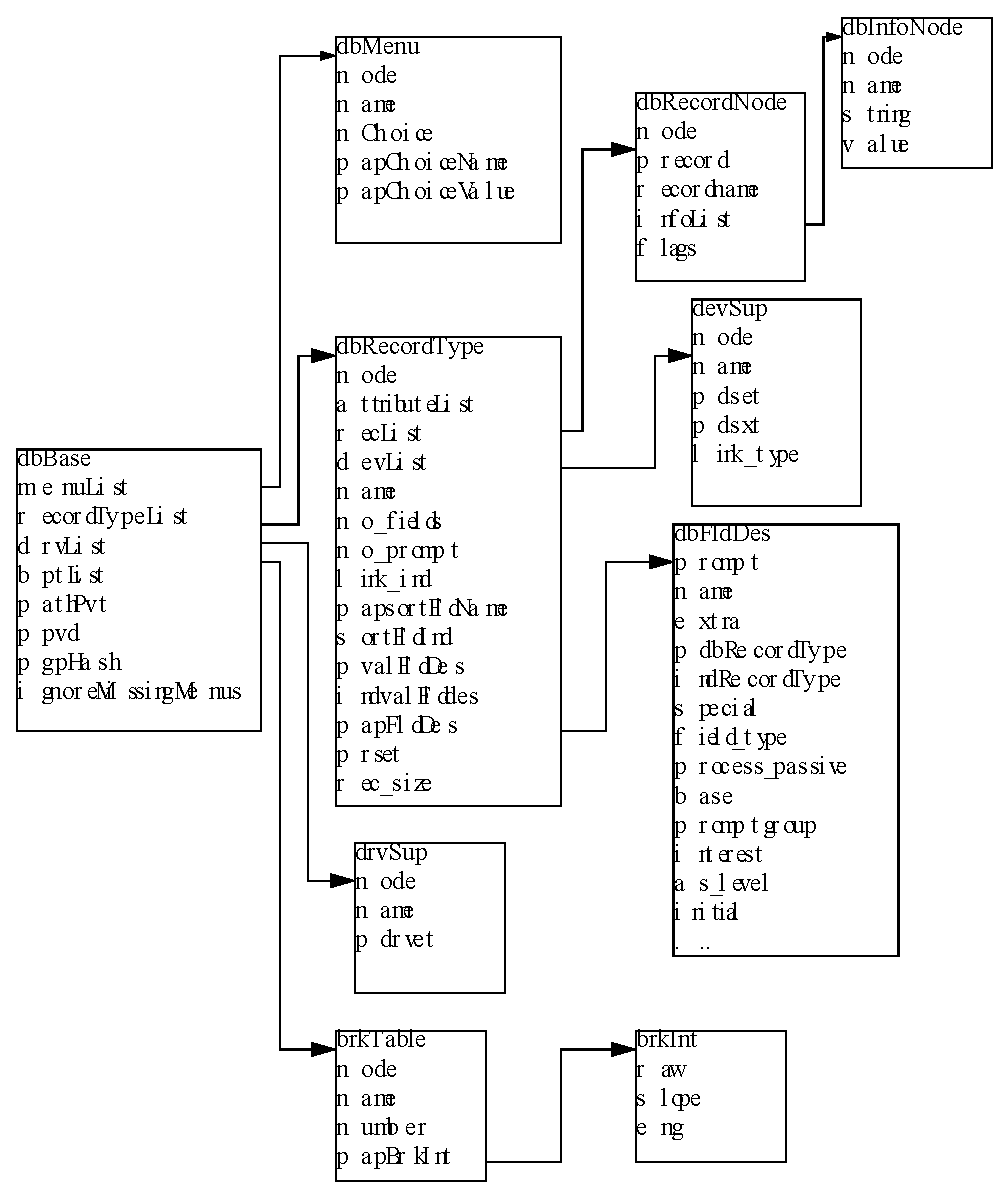
\includegraphics{databaseStructures_1}










\chapter*{Index}
\addcontentsline{toc}{chapter}{Index}
\printindex


\end{document}

